\documentclass[a4paper, twoside, openright]{report}

% some page formatting packages
\linespread{1.3} % line spacing for when it becomes necessary
\usepackage{parskip}
\usepackage[inner=3cm, outer=2cm, bottom=2cm]{geometry}
\usepackage{lscape}
\pagestyle{headings}
\usepackage{microtype} % prettyfication
\usepackage{emptypage} % remove headers from empty pages

\makeatletter
\renewcommand{\maketitle}
{
	\begin{titlepage}
		\begin{center}
			
\includegraphics[width=0.15\textwidth]{Images/BCU.jpg} \\
			\vspace{0.5em}
			{\huge Digital Media Technology Lab} \\
			\vspace{0.5em}
			{\huge Birmingham City University} \\
			\vspace{14em}
			{\bfseries \Huge \@title} \\
			\vspace{3em}
			{\huge \@author} \\
			\vspace*{\fill}
			{\Large A thesis submitted in partial fulfilment of the requirements for the degree of Doctor of
			Philosophy, \@date}
		\end{center}
	\end{titlepage}
}
\makeatother

% let's try and make the paragraph spacing look good
\setlength{\parskip}{5pt plus 0pt minus 0pt}
\setlength{\parsep}{12pt plus 3pt minus 0pt}
\setlength{\headsep}{25pt}
\setlength{\topskip}{0pt}
\setlength{\topmargin}{0pt}
\setlength{\topsep}{0pt}
\setlength{\partopsep}{0pt}
\setlength{\textfloatsep}{15pt plus 0pt minus 0pt}
\setlength{\floatsep}{15pt plus 0pt minus 0pt}
\setlength{\intextsep}{12pt plus 0pt minus 0pt}
\usepackage[compact]{titlesec}
\titlespacing{\section}{0pt}{20pt plus 0pt minus 0pt}{*0}
\titlespacing{\subsection}{0pt}{12pt plus 0pt minus 0pt}{*0}
\titlespacing{\subsubsection}{0pt}{12pt plus 0pt minus 0pt}{*0}

% tell tex that widows and orphans are bad
\usepackage[all]{nowidow}

% abstract stuff
\renewenvironment{abstract}
{
	\cleardoublepage
	\phantomsection
	\addcontentsline{toc}{chapter}{Abstract}
	\thispagestyle{plain}
	\setcounter{page}{1}
	\vspace*{\fill}
	\begin{center}
		{\bfseries \Large Abstract}
	\end{center}
}
{
	\vspace*{\fill}
}

% acknowledgements stuff
\newenvironment{acknowledgements}
{
	\cleardoublepage
	\phantomsection
	\addcontentsline{toc}{chapter}{Acknowledgements}
	\thispagestyle{plain}
	\vspace*{\fill}
	\begin{center}
		{\bfseries \Large Acknowledgements}
	\end{center}
}
{
	\vspace*{\fill}
}

% packages for figures
\usepackage[pdftex]{graphicx}
\usepackage{subfig}
\usepackage[justification=centering]{caption}
\usepackage{epstopdf}

% data float type
\usepackage{float}
\newfloat{datum}{htbp}{lod}[chapter]
\floatname{datum}{Datum}
\newsubfloat{datum}

\makeatletter
\renewcommand*{\listof}[2]{
	\@ifundefined{ext@#1}{\float@error{#1}}{
		\@namedef{l@#1}{\@dottedtocline{1}{0em}{2.3em}}
		\float@listhead{#2}
		\begingroup\setlength{\parskip}{\z@}
			\@starttoc{\@nameuse{ext@#1}}
		\endgroup}}
\makeatother

% don't indent lists of figures or tables
\makeatletter
\renewcommand*\l@figure{\@dottedtocline{1}{0em}{2.3em}}
\let\l@table\l@figure
\makeatother

% oh yes we have to use Harvard referencing or Peter will kill us
\usepackage{natbib}
\usepackage{bibentry}
\nobibliography*

% packages for the formatting of equations
\usepackage{amsmath}
\DeclareMathOperator{\sgn}{sgn}
\newcommand{\floor}[1]{\left\lfloor#1\right\rfloor}
\newcommand{\ceil}[1]{\left\lceil#1\right\rceil}
\newcommand{\round}[1]{\left\lfloor#1\right\rceil}
\newcommand{\abs}[1]{\left|#1\right|}
\newcommand{\euclidian}[1]{\left|\left|#1\right|\right|}
\newcommand{\medcap}{\mathbin{\raisebox{\depth}{\scalebox{0.75}{\ensuremath{\bigcap}}}}}
\newcommand{\medcup}{\mathbin{\raisebox{\depth}{\scalebox{0.75}{\ensuremath{\bigcup}}}}}
\usepackage{amsfonts}
\usepackage{mathabx}

% make some colours and commands so we can put in notes to ourself
\usepackage{color}
\definecolor{noteColour}{RGB}{0, 0, 255}
\definecolor{todoColour}{RGB}{255, 0, 0}
\newcommand{\note}[1]{{\color{noteColour}#1}}
\newcommand{\todo}[1]{{\color{todoColour}#1}}

% sub/superscript commands
\newcommand{\sub}[1]{\textsubscript{#1}}
\newcommand{\super}[1]{\textsuperscript{#1}}

% clickable links for references in the document also put page cited on info in the bibliography
\usepackage[backref=page]{hyperref}
\hypersetup
{
	colorlinks,
	citecolor=black,
	filecolor=black,
	linkcolor=black,
	urlcolor=black
}
\renewcommand*{\backref}[1]{}
\renewcommand*{\backrefalt}[4]
{
	\ifcase #1 [Not Cited.]
	\or [Cited on Page #2.]
	\else [Cited on Pages #2.]
	\fi
}

% gotta draw them diagrams in tikz, otherwise you fail at life
\usepackage{tikz}
\usetikzlibrary{fit, arrows, shapes, patterns, positioning}
\tikzstyle{dots} = [dotted]
\tikzstyle{operator} = [circle, draw=black]
\tikzstyle{gain} = [regular polygon, regular polygon sides=3, inner sep=0, draw=black, shape border rotate=270,
                    minimum size=2em]

% fuck serifs
\renewcommand{\familydefault}{\sfdefault}

% allow for referencing enums
\usepackage{enumitem}

% make those tables pretty
\usepackage{array}
\usepackage{hhline}
\usepackage{longtable}
\newcolumntype{C}[1]{>{\centering}p{#1}}
\setlength{\LTpre}{8pt}
\setlength{\LTpost}{8pt}

% appendices :(
\usepackage[toc]{appendix}

% glossary options
\usepackage[acronym, nonumberlist, nomain, toc, style=alttree]{glossaries}
\newglossary[mlg]{maths}{mni}{mno}{Mathematical Notation}
\glssetwidest[0]{MUSHRAAAA}
\renewcommand{\glstreenamefmt}{}
\makeglossaries

% glossary entries
\newacronym{adsr}{ADSR}{Attack, Decay, Sustain, Release}
\newacronym{pmf}{PMF}{Probability Mass Function}
\newacronym{dft}{DFT}{Discrete Fourier Transform}
\newacronym{dct}{DCT}{Discrete Cosine Transform}
\newacronym{stft}{STFT}{Short-Time Fourier Transform}
\newacronym{mfcc}{MFCC}{Mel Frequency Cepstral Coefficient}
\newacronym{mds}{MDS}{Multidimensional Scaling}
\newacronym{pca}{PCA}{Principal Component Analysis}
\newacronym{pc}{PC}{Principal Component}
\newacronym{efa}{EFA}{Exploratory Factor Analysis}
\newacronym{lti}{LTI}{Linear Time Invariant}
\newacronym{ltv}{LTV}{Linear Time Variant}
\newacronym{thd}{THD}{Total Harmonic Distortion}
\newacronym{imd}{IMD}{Intermodulation Distortion}
\newacronym{ssba}{SSBA}{Single Sideband Automodulation}
\newacronym{iap}{IAP}{Instantaneous Amplitude and Phase}
\newacronym{sttr}{STTR}{Short-Time Time Reversal}
\newacronym{daw}{DAW}{Digital Audio Workstation}
\newacronym{fir}{FIR}{Finite Impulse Response}
\newacronym{iir}{IIR}{Infinte Impulse Response}
\newacronym{vame}{VAME}{Verbal Attribute Magnitude Estimation}
\newacronym{mushra}{MUSHRA}{Multiple Stimuli with Hidden Reference and Anchor}
\newacronym{api}{API}{Application Programming Interface}
\newacronym{safe}{SAFE}{Semantic Audio Feature Extraction}
\newacronym{lfo}{LFO}{Low Frequency Oscillator}
\newacronym{erb}{ERB}{Equivalent Rectangular Bandwidth}
\newacronym{vst}{VST}{Virtual Studio Technology}
\newacronym{au}{AU}{Audio Unit}
\newacronym{rdf}{RDF}{Resource Description Framework}
\newacronym{eq}{EQ}{Equaliser}
\newacronym{amdf}{AMDF}{Average Magnitude Difference Function}
\newacronym{hps}{HPS}{Harmonic Product Spectrum}

\newglossaryentry{maths:round}
{
	type=maths,
	name={$\round{a}$},
	description={$a$ rounded to the nearest integer},
	sort={round}
}
\glsadd{maths:round}

\newglossaryentry{maths:divides}
{
	type=maths,
	name={$a \divides b$},
	description={$a$ divides $b$, i.e. $\dfrac{b}{a}$ is an integer.},
	sort={divides}
}
\glsadd{maths:divides}

\newglossaryentry{maths:signum}
{
	type=maths,
	name={$\sgn(a)$},
	description={the signum funciton (the sign of $a$), $1$ for $a > 0$, $-1$ for $a < 0$, $0$ for $a = 0$},
	sort={fsignum}
}
\glsadd{maths:signum}

\newglossaryentry{maths:max}
{
	type=maths,
	name={$\displaystyle \max_{i = 0}^{I} A_{i}$},
	description={the maximum value of $A_{i}$ for $0 \leq i \leq I$},
	sort={nmax}
}
\glsadd{maths:max}

\newglossaryentry{maths:matrixrow}
{
	type=maths,
	name={$\mathbf{D}_{i*}$},
	description={the $i$\super{th} row of matrix $\mathbf{D}$},
	sort={matrixi}
}
\glsadd{maths:matrixrow}

\newglossaryentry{maths:matrixcolumn}
{
	type=maths,
	name={$\mathbf{D}_{*j}$},
	description={the $j$\super{th} column of matrix $\mathbf{D}$},
	sort={matrixj}
}
\glsadd{maths:matrixcolumn}

\newglossaryentry{maths:matrixtranspose}
{
	type=maths,
	name={$\mathbf{D}^{T}$},
	description={the transpose of matrix $\mathbf{D}$},
	sort={matrixtranspose}
}
\glsadd{maths:matrixtranspose}

\newglossaryentry{maths:matrixinverse}
{
	type=maths,
	name={$\mathbf{D}^{-1}$},
	description={the inverse of matrix $\mathbf{D}$},
	sort={matrixnverse}
}
\glsadd{maths:matrixinverse}

\newglossaryentry{maths:euclidian}
{
	type=maths,
	name={$\euclidian{a - b}$},
	description={the Euclidian distance between two points, $a$ and $b$, in a multidimensional space},
	sort={euclidian}
}
\glsadd{maths:euclidian}

\newglossaryentry{maths:mahalanobis}
{
	type=maths,
	name={$M(x, d)$},
	description={the Mahalanobis distance between a point, $x$, and a distribution, $d$, in a multidimensional space},
	sort={eumahal}
}
\glsadd{maths:mahalanobis}

\newglossaryentry{maths:setcomp}
{
	type=maths,
	name={$A \setminus B$},
	description={the relative complement of set $B$ with respect to set $A$ (the set of elements in $A$ which are not in
		     $B$)},
	sort={sxetcomp}
}
\glsadd{maths:setcomp}

\newglossaryentry{maths:subset}
{
	type=maths,
	name={$A \subseteq B$},
	description={$A$ is a subset of or equal to $B$ ($A$ only contain elements which are also in $B$)},
	sort={subset}
}
\glsadd{maths:subset}

\newglossaryentry{maths:setunion}
{
	type=maths,
	name={$A \protect\medcup B$},
	description={the union of sets $A$ and $B$ (the set which contains all elements in both $A$ and $B$)},
	sort={setunion}
}
\glsadd{maths:setunion}

\newglossaryentry{maths:setmembership}
{
	type=maths,
	name={$a \in A$},
	description={set membership, $a$ is an element of $A$},
	sort={setmembership}
}
\glsadd{maths:setmembership}

\newglossaryentry{maths:thenaturalnumbers}
{
	type=maths,
	name={$\textbf{N}$},
	description={the set of all natural numbers (integers greater than zero)},
	sort={thenaturalnumbers}
}
\glsadd{maths:thenaturalnumbers}

\newglossaryentry{maths:theintegers}
{
	type=maths,
	name={$\textbf{Z}$},
	description={the set of all integers},
	sort={theintegers}
}
\glsadd{maths:theintegers}

\author{Sean Enderby}
\title{Timbral Control of Audio Through Harmonic Excitation}
\date{November 2017} % fill that shit in when i'm done

\begin{document}
% display parameters need to go in here
\setlength{\abovedisplayskip}{0pt plus 0pt minus 0pt}
\setlength{\belowdisplayskip}{12pt plus 0pt minus 0pt}
\setlength{\abovedisplayshortskip}{0pt plus 0pt minus 0pt}
\setlength{\belowdisplayshortskip}{12pt plus 0pt minus 0pt}

\pagenumbering{roman}
\maketitle

%\begin{center}
%	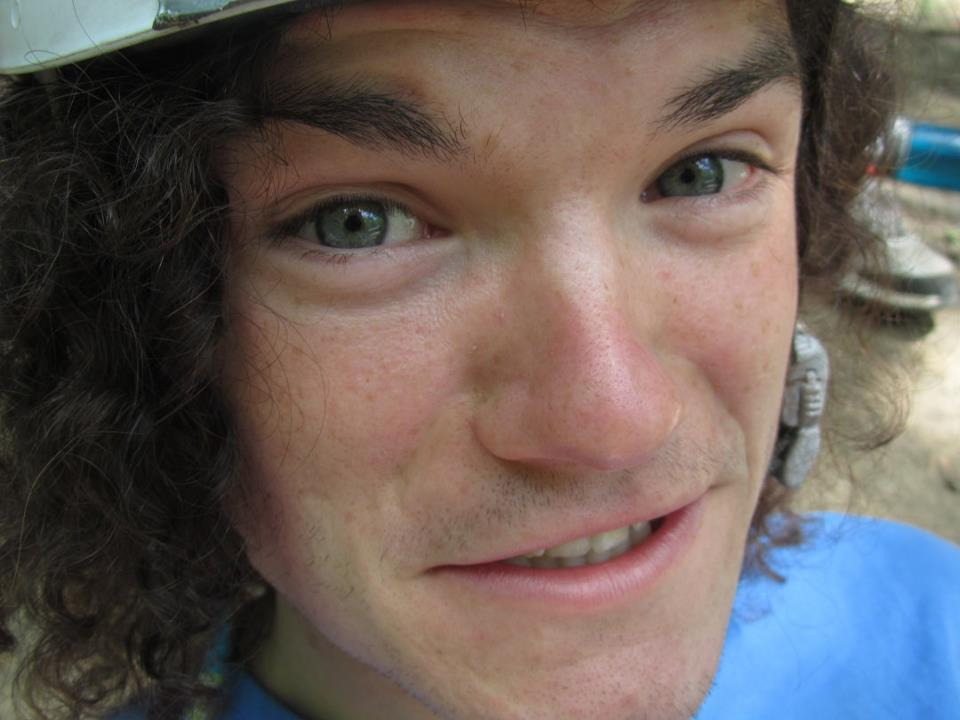
\includegraphics[width=0.8\textwidth]{Images/seanFace.jpg}
%	\newline
%	\newline
%	\Huge
%	Welcome to my thesis, are your ready for some fun?
%	\normalsize
%\end{center}

\begin{abstract} 
	Timbre is the property of a sound which allows it to be distinguished from other sounds of the same loudness and
	pitch. These differences can also be demonstrated mathematically as differences in low level signal features.
	Research into timbre typically focuses on analysing the multidimensional relationship between these low level
	features and the perceived timbre. In music production the timbre of recorded sounds is altered through the
	application of audio effects. A commonly used class of audio effects is harmonic excitation, in which new spectral
	content is introduced to the signal at harmonic frequencies. This thesis focuses on the uses of harmonic excitation
	effects for the control of timbre. For a harmonic excitation system to provide control over the timbre of a signal
	it must be able to manipulate the associated low level features. As such, various harmonic excitation algorithms are
	evaluated against a set of criteria which describe how well they are suited to applying timbral control, methods
	which allow for the generation of individual harmonics being shown to provide the most flexibility. Techniques are
	then developed by which these algorithms can be used to provide monotonic control over various low level features of
	audio signals. 

	It is often necessary to discuss these timbral manipulations using semantic descriptors (e.g. `warm' and `bright').
	The timbral meanings of these terms can be discerned through analysis of the relationship between their use to
	describe audio signals and the signal's low level features. To investigate these relationships a study is conducted
	analysing the changes to perceived timbre and audio features associated with the application of distortion and
	equalisation effects. Four distinct timbral groups are identified (warmth, brightness, crunchiness and muddiness)
	each consisting of related semantic terms. The meanings of these semantic groups are uncovered by measuring how the
	low level features of signals are manipulated by the application of the effects. The distinction between each of the
	groups are found to be highly correlated with several low level audio features.
	
	Significant experience is required to be able to utilise traditional studio equipment to manipulate the timbre of a
	sound based on a semantic description. Recently, new tools have been developed which have control parameters
	labelled with commonly used timbral descriptors, reducing the amount of experience needed. These systems manipulate
	the low level features of a signal associated with a particular timbral group. In this work two such systems are
	proposed utilising harmonic excitation algorithms. One moving audio between the warmth and brightness timbral groups
	and the other between the brightness and crunchiness groups. Subjective listening tests are conducted to evaluate
	the performance of these systems. Both are successful in processing audio such that is is perceived as part of the
	brightness group, participants exhibiting a minimum accuracy of 72\% in identifying the timbral group. When
	configured to introduce warmth or crunchiness the systems perform less well, participants only identifying the
	correct timbral group 54\% or 51\% of the time respectively.
\end{abstract}

\tableofcontents
\listoffigures
\listoftables
\listof{datum}{List of Data}

\pagenumbering{arabic}
%\setcounter{chapter}{0}
\chapter{Introduction}
\label{chap:Introduction}

\section{Motivation}
\label{sec:Introduction-Motivation}
% Genuine Waffle (if those who disagree have uncovered this comment I have no regrets)
	The process of music production can be split into four main stages (recording, editing, mixing and mastering) as
	shown in Figure~\ref{fig:MusicProduction}. In the recording stage, acoustic and digital sound sources are captured,
	resulting in a set of recorded audio signals (often called stems). These are then edited to correct any mistakes
	made during the recording and to arrange them in time, forming the musical structure of the finished piece. The
	signals are then processed further and mixed together to produce the final product.

	\begin{figure}[h!]
		\centering
		\begin{tikzpicture}
			\node (Sources) [align=center] at (0, 0) {Sound\\Sources};
			\node (Mic1) [draw] at (2, 1.5) {Microphone};
			\node (Mic2) [draw] at (2, 0.5) {Microphone};
			\node (Mic3) [draw] at (2, -0.5) {Microphone};
			\node (Mic4) [draw] at (2, -1.5) {Microphone};

			\draw [dots] (3.2, 3) -- (3.2, -2);
			\node (Recording) at (2, 2.5) {\bf{Recording}};

			\node (Edit1) [draw] at (4.5, 1.5) {Editing Tools};
			\node (Edit2) [draw] at (4.5, 0.5) {Editing Tools};
			\node (Edit3) [draw] at (4.5, -0.5) {Editing Tools};
			\node (Edit4) [draw] at (4.5, -1.5) {Editing Tools};

			\draw (Mic1) -- (Edit1);
			\draw (Mic2) -- (Edit2);
			\draw (Mic3) -- (Edit3);
			\draw (Mic4) -- (Edit4);

			\draw [dots] (5.8, 3) -- (5.8, -2);
			\node (Editing) at (4.5, 2.5) {\bf{Editing}};

			\node (Proc1) [draw] at (6.9, 1.5) {Processing};
			\node (Proc2) [draw] at (6.9, 0.5) {Processing};
			\node (Proc3) [draw] at (6.9, -0.5) {Processing};
			\node (Proc4) [draw] at (6.9, -1.5) {Processing};

			\draw (Edit1) -- (Proc1);
			\draw (Edit2) -- (Proc2);
			\draw (Edit3) -- (Proc3);
			\draw (Edit4) -- (Proc4);

			\node (Mixer) at (9.1, 0) {Mixer};
			\draw (8.2, 1.8) rectangle (10, -1.8);
			\coordinate (Mix1) at (8.2, 1.5);
			\coordinate (Mix2) at (8.2, 0.5);
			\coordinate (Mix3) at (8.2, -0.5);
			\coordinate (Mix4) at (8.2, -1.5);

			\node (Mixing) at (8, 2.5) {\bf{Mixing}};

			\draw (Proc1) -- (Mix1);
			\draw (Proc2) -- (Mix2);
			\draw (Proc3) -- (Mix3);
			\draw (Proc4) -- (Mix4);

			\draw [dots] (10.2, 3) -- (10.2, -2);
			\node (Mastering) at (11.3, 2.5) {\bf{Mastering}};

			\node (Master) [draw] at (11.3, 0) {Processing};
			\draw (10, 0) -- (Master);

			\node (Mix) [align=center] at (13.2, 0) {Finished\\Product};
			\draw (Master) -- (Mix);
		\end{tikzpicture}
		\caption{A block diagram of the music production process.}
		\label{fig:MusicProduction}
	\end{figure}

	During the mixing and mastering stages, audio effects are used to creatively shape the timbre of recorded audio
	signals. This is represented by the blocks labelled `Processing' in Figure~\ref{fig:MusicProduction}. This allows
	producers to create timbres which are not possible to achieve through only the recording of acoustic instruments.
	Traditional audio effects evolved from the use of analogue signal processing systems designed to address the
	technical requirements of broadcast or recording. As such, these effects have control parameters which relate
	directly to specific technical properties of an audio signal: a traditional equaliser has parameters for selecting
	specific frequency regions, traditional dynamics processors (compressors and limiters) have parameters relating to
	signal amplitudes. These parameters are effective when correcting technical issues with a signal but do not allow
	for intuitive creative manipulation of timbre.

	The application of audio effects for creative purposes is typically motivated by the perceived timbre of the audio.
	Creative decisions are often expressed using language which does not refer to the mathematical properties of the
	recorded signals. For example, one might ask that the saxophone is made more present in the mix, or that the piano
	be made to sound more airy. In order to complete these tasks using traditional audio effects, music producers and
	audio engineers require knowledge of how the technical parameters of the effect relate to specific perceived aspects
	of timbre. This knowledge is gained through training and experience, presenting an obstacle to novices.

	Audio production software typically uses parameter presets to assist novice users. These are a predefined set of
	parameter values for a particular effect which are labelled with semantic descriptions. Users can apply an effect to
	a signal and choose a preset which best fits their desired outcome. This does not, however, provide an intuitive
	interface to the user. A static parameter setting will not apply the same timbral transformation to all input
	signals. If the user wishes to alter the settings slightly, they still require knowledge of how the effect's
	parameters relate to perceived timbre. For example, a user might apply a preset to make a sound brighter; if they
	are not happy with the result, no assistance is given in making the sound more or less bright.

	More intuitive interfaces for control over timbre provide parameters which directly relate to perceived aspects of a
	sound. These perform the translation between the language used to describe timbre and the technical parameters of
	signal processing algorithms, allowing users to focus on the creative aspects of music production. Having timbral
	properties controlled by continuous parameters increases the intuitiveness of the system as it is evident which
	parameter to adjust to change a particular timbral property. The effect can also analyse the input signal and adjust
	itself such that the parameter has similar timbral effects across a wide range of inputs. Developing this type of
	semantically controlled effect requires study of how the mathematical properties of a signal contribute to its
	perceived timbre. Effects can then be built which manipulate these signal properties according to the value of a
	semantically labelled parameter. Making audio effects more intuitive in this manner aids both novice and experienced
	music producers and audio engineers. Novices benefit from the reduced amount of knowledge needed to apply audio
	effects; being able to select and adjust effects based on natural language descriptions of timbre rather than
	requiring a technical knowledge of signal processing. For experienced users these effects can be used to accelerate
	the production process; reducing the work required to configure audio effect parameters, allowing users to focus on
	creative decisions. 
	
	Commercial audio effects with semantically labelled parameters have been available for a number of years, for
	example the OneKnob series of effects produced by \citet{wavesoneknob}. Being commercial products, the operation of
	these effects is not known, but it is assumed that they were developed alongside input from professional audio
	engineers. In academic research, a number of studies have been undertaken in developing these types of control
	systems for synthesis and audio processing applications (discussed in Section~\ref{sec:Timbre-Control}). This work
	focusses on how this type of system can be built using nonlinear distortion / excitation effects.

\section{Objectives and Research Questions}
\label{sec:Introduction-Objectives}
	The underlying objective of this thesis is to produce intuitive timbre shaping effects based on harmonic excitation
	algorithms (systems which introduce new harmonic partials to a signal). This is achieved through answering the
	following questions:

	\begin{itemize}
		\item What semantic terms are commonly used to describe the timbre of harmonic excitation effects? 
		\item What properties of audio signals contribute to these timbral descriptions and what alterations are
		      made to signals to produce a certain timbral result?
		\item What properties of audio signals can be reliably controlled by harmonic excitation algorithms?
		\item How can harmonic excitation systems be configured to control elements of timbre? Systems will be
		      proposed which allow control over particular semantic features and the accuracy of these systems
		      assessed.
		\item Can harmonic excitation be used to provide intuitive control of timbre? Do the proposed systems
		      provide control over the aspects of timbre they are designed to?
	\end{itemize}

\section{Thesis Structure}
\label{sec:Introduction-ThesisStructure}
	The aim of this work is to develop harmonic excitation systems which provide intuitive control over timbre.
	Firstly, a review of the existing work in timbral manipulation and nonlinear processing is given. Experiments are
	then conducted to discover how spectral manipulations are used in music production. This information is used to aid
	in the design of semantically controlled harmonic excitation effects which are subsequently evaluated in perceptual
	listening tests. This is presented in seven chapters as follows:

	In {\bf{Chapter~\ref{chap:Timbre}}} the background of research into timbre is discussed. It begins with a discussion
	of the low level features of audio signals. Popular experimental methodologies for uncovering the perceptual effects
	of these features are then introduced, along with the methods used to analyse their results. Finally, existing work
	concerning the control of perceptual features of audio signals is discussed.

	{\bf{Chapter~\ref{chap:Excitation}}} covers the body of work concerning harmonic excitation, starting with a
	discussion of the analysis of nonlinear systems in the field of audio production. The uses of such systems and their
	timbral effects are then presented. Finally, various algorithms for harmonic excitation, proposed in existing
	literature, are described.

	In {\bf{Chapter~\ref{chap:TimbreEvaluation}}} the collection of semantic audio data during the music production
	process is discussed. This data is used to determine the language used for describing audio in a studio environment
	and how audio effects are used to evoke certain timbral descriptors.

	In {\bf{Chapter~\ref{chap:ExcitationEvaluation}}} a set of criteria for assessing the applicability of harmonic
	excitation techniques to timbral control is proposed. The algorithms described in Chapter~\ref{chap:Excitation} are
	then evaluated against these criteria to identify those most suitable for use in timbral control systems.  Methods
	by which the performance of certain harmonic excitation methods can be improved are proposed.

	In {\bf{Chapter~\ref{chap:FeatureControl}}} results from Chapter~\ref{chap:ExcitationEvaluation} are used to inform
	the design of systems for controlling low level audio features using harmonic excitation techniques. Systems are
	developed which can be used to provide monotonic control over a specific low level feature of the input signal. The
	operation of these systems is evaluated using a number of test signals.

	In {\bf{Chapter~\ref{chap:PerceptualExperiments}}} the systems proposed in Chapter~\ref{chap:FeatureControl} are
	refined, using the results of Chapter~\ref{chap:TimbreEvaluation}, to develop harmonic excitation effects which
	control specific timbral traits of a signal. These effects are evaluated objectively, through comparison with the
	dataset gathered in Chapter~\ref{chap:TimbreEvaluation}; and subjectively, through a series of perceptual listening
	tests.

	The thesis is concluded in {\bf{Chapter~\ref{chap:Conclusion}}} with a summary of findings across Chapters
	\ref{chap:TimbreEvaluation} to \ref{chap:PerceptualExperiments}, a critique of the methods used in this work and
	suggestions for further work in this area.

\section{Contributions}
\label{sec:Introduction-Contributions}
	The primary contribution of this thesis is the proposal of methods by which harmonic excitation systems can be
	configured to give intuitive control over timbral features. In achieving this a number of other contributions are
	made, as follows:

	\begin{itemize}
		\item a new method for the collection of semantic audio descriptors and their underlying features
		      (Chapter~\ref{chap:TimbreEvaluation})
		\item a new metric for the measurement of agreement in multidimensional distributions
		      (Chapter~\ref{chap:TimbreEvaluation})
		\item a methodology for the assessment of harmonic generation algorithms for use in timbral control
		      (Chapter~\ref{chap:ExcitationEvaluation})
		\item a comparison of harmonic generation algorithms and their suitability to provide perceptual control
		      (Chapter~\ref{chap:ExcitationEvaluation})
		\item the development of new harmonic excitation systems for control of low level audio features
		      (Chapter~\ref{chap:FeatureControl})
		\item new methods for controlling perceptual attributes of audio using harmonic excitation
		      (Chapter~\ref{chap:PerceptualExperiments})
	\end{itemize}

	The following papers have been published as part of this work:

	\begin{itemize}
		\item \bibentry{enderby2012harmonic}
		\item \bibentry{enderby2013methods}
		\item \bibentry{stables2014safe}
		\item Enderby, S. and Stables, R. (September 2017), A Nonlinear Method for Manipulating Warmth and
		      Brightness, in \emph{Proceedings of the International Conference on Digital Audio Effects (DAFx-17)}
	\end{itemize}

	Other associated publications include:

	\begin{itemize}
		\item Ward, D., Enderby, S., Athwal, C. and Reiss, J. (December 2015), Real-Time Excitation Based Binaural
		      Loudness Meters, in \emph{Proceedings of the International Conference on Digital Audio Effects
		      (DAFx-15)}
		\item Stables, R., De Man, B., Enderby, S., Reiss, J., Fazekas, G. and Wilmering, T. (October 2016),
		      Semantic Description of Timbral Transformations in Music Production, in \emph{Proceedings of the
		      2016 ACM on Multimedia Conference}
		\item Stasis, S., Jillings, N., Enderby, S. and Stables, R. (September 2017), Audio Processing Chain
		      Recommendation, in \emph{Proceedings of the International Conference on Digital Audio Effects
		      (DAFx-17)}
	\end{itemize}

%Review of timbral control research.
%	Timbre Definition
%	Timbre Spaces (MDS and shit)
%	Audio Features
%	Perceptual Control of Synthesis

\chapter{Timbre}
\label{chap:Timbre}
	There are three properties which describe how a sound is perceived, these being loudness, pitch and timbre. Loudness
	describes the perceived intensity of a sound and pitch its perceived frequency. Timbre then describes any other
	properties of a sound, besides loudness and pitch, which allow it to be distinguished from other sounds
	\citep{mathews1999introduction}. Loudness and pitch are both one dimensional properties allowing sounds to be
	ordered from quiet to loud or low to high pitch. Timbre is a more complex property consisting of multiple dimensions
	\citep{rossing2002the}. There is a large body of research concerning the analysis of timbre, identifying these
	dimensions and their relationships with the acoustic features of a sound.

	Simple descriptions of a sounds timbre involve instrument identification. A sound could be described as `cello-like'
	or `flute-like'. More broadly the class of instrument, string or woodwind, could be used to describe the timbre of a
	sound. While these terms are useful for discussing the instrumentation of pieces they can not be applied generally
	to a wide range of timbres. It is not very useful to describe the timbre of a xylophone as being `not flute-like'.

	More general timbral descriptors directly describe the sound itself rather than the source which produced it. These
	include terms such as bright, rough and sharp. This allows the timbre of different sounds to be compared according
	to these terms \citep{howard2009acoustics}. Sounds can also be ordered in respect to these criteria much like with
	loudness and pitch. For example one could order a set of sounds by how bright they sound.

	Early research into timbre was performed by \citet{helmholtz1875on}. More recent work involves research from various
	fields. Low level features of audio segments can be found using signal analysis techniques. More complicated
	information about the perception of a signal can be discovered through modelling the behaviour of the human hearing
	system. Lastly experiments can be undertaken in which participants listen to audio samples and provide responses
	regarding the timbre of the samples. These responses are then analysed to uncover any correlations between the
	participants responses and lower level features of the audio samples.

	This chapter will review the existing body of timbral research. Section \ref{sec:Timbre-LowLevelFeatures} discusses
	metric which are used to describe the low level features of audio signals. Section
	\ref{sec:Timbre-PsychoacousticPrinciples} covers various models which describe the perception of various auditory
	phenomena. \note{Put in what the rest of the sections are about}.

\section{Low Level Audio Features}
\label{sec:Timbre-LowLevelFeatures}
	A widely cited definition of timbre \citep{ASA1960american} suggests that timbre in influenced by various low level
	features of an audio signal. The spectral content, waveform and temporal characteristics all effect the perceived
	timbre of a sound. Signal analysis techniques can be used to extract information about these elements of a signal.
	A large list of such features feature extraction techniques is given by \citep{peeters2004a}. These features can be
	separated into three categories. Features which describe the properties of a signals waveform and how it evolves
	with time (temporal features), features which describe the frequency content of a signal (spectral features) and
	features which describe how the frequency content of a signal evolves with time (spectro-temporal features).

	\subsection{Temporal Features}
	\label{sec:Timbre-LowLevelFeatures-Temporal}
		Simple temporal features involve taking statistical measurements, such as mean and variance, of the audio
		samples in a signal. These measures give basic information about the level and variation in a signal but in
		many cases they do not represent a signals properties very well. For example, the mean value of a sinusoidal
		signal over a whole number of cycles is zero. 

		A common technique to extract more meaningful information about a signals level is to use an envelope
		detector. 

		\begin{figure}[h!]
			\centering
			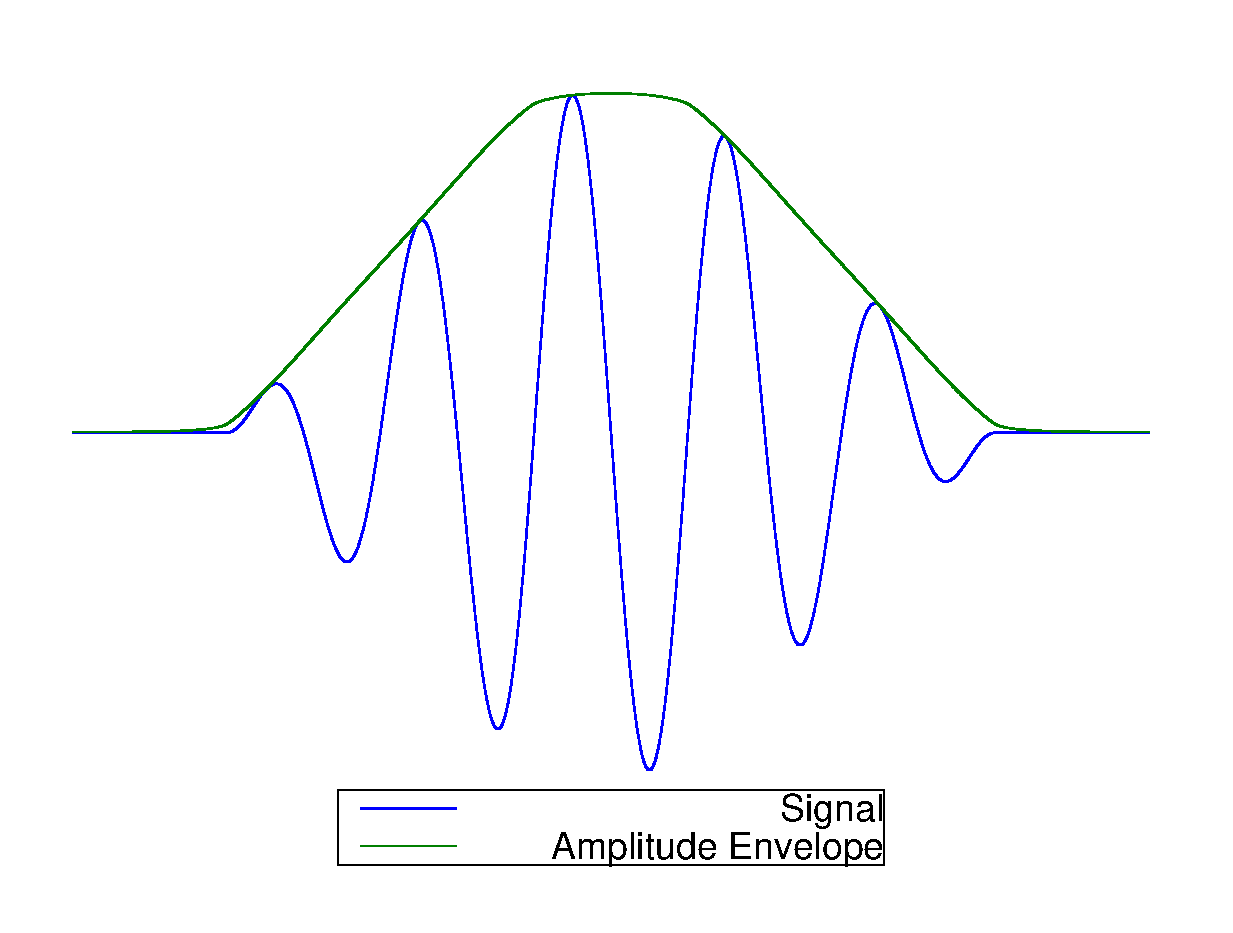
\includegraphics[width=0.6\textwidth]{chapter2/Images/AmplitudeEnvelope.eps}
			\caption{The Amplitude Envelope of a Signal.}
			\label{fig:AmplitudeEnvelope}
		\end{figure}

		\note
		{
			Envelope Detection (ADSR). Methods reviewed by \citet{chang2007a}.
		}

	\subsection{Spectral Features}
	\label{sec:Timbre-LowLevelFeatures-Spectral}
		\note
		{
			\begin{itemize}
				\item Spectral statistics.
				\item Spectral shape.
				\item MFCCs.
			\end{itemize}

			MFCCs originally developed for speech recognition \citep{davis1980comparison} but used for other
			timbral tasks more recently \citep{depoli1997sonological}.
		}

	\subsection{Spectro-Temporal Features}
	\label{sec:Timbre-LowLevelFeatures-Spectrotemporal}
		\note
		{
			Delta MFCC and spectral flux and such and the like.
		}

	\note
	{
		Stuff like this also \citep{freed1990auditory, lakatos2000a}.
	}
	
\section{Psychoacoustic Principles}
\label{sec:Timbre-PsychoacousticPrinciples}
	Psychoacoustics is a field which deals with the perception of sound. The existing literature concerns the study of
	the human hearing system and how it responds to certain aspects of audio stimuli. Several different areas of audio
	perception have been researched. Methods have been devised to model the human perception of loudness
	\citep{moore1997a} and pitch \citep{gerhard2003pitch}. Other research considers the human hearing systems ability to
	locate sound sources \citep{blauert1997spatial}. This section will summarise the psychoacoustic principles which are
	useful for investigating the perception of timbre. 

	\note
	{
		Critical bands and masking.

		Resolving harmonics in the cochlea. Low order harmonics are generally resolved individually so their
		individual levels will have a strong effect on perceived timbre. Higher order harmonics are resolved in
		groups so less manipulation is needed \citep{howard2009acoustics}.
	}

\section{Timbral Features}
\label{sec:Timbre-TimbralFeatures}
	\note
	{
		Psychoacoustic principles have been used to develop timbral metrics (sharpness, roughness).
	}

\section{Parameterisation of Timbre}
\label{sec:Timbre-Parameterisation}
	\note{Analysis of timbre spaces and discussion on salience of some features as given in the literature.}

	\subsection{Dissimilarity Tests}
	\label{sec:Timbre-Dissimilarity}
		\note
		{
			A more traditional approach, \citet{grey1977multidimensional} and all the copycat lot 
			\citep{burgoyne2008a, caclin2005acoustic}.
		}

	\subsection{VAME}
	\label{sec:Timbre-VAME}
		\note{\citet{kendall1993verbal1, kendall1993verbal2} trying to upset the status quo.}

	\subsection{Parameter Space}
	\label{sec:Timbre-ParameterSpaces}
	\note{Research like Social EQ and stuff \citep{cartwright2013socialeq, seetharaman2014crowdsourcing}.}

\section{Controlling Timbre}
\label{sec:Timbre-Control}
	\note{Lots of them synthesis dudes have tried to control the beast. \citet{zacharakis2011an} did some stuff.}
	
	\note
	{
		Some dudes do morphing (analysis resynthesis from what I remember) like good old 
		\citet{williams2007perceptually, williams2009perceptually, williams2010perceptually}
	}

%Review of existing harmonic excitation.
%	Nonlinear Systems
%		Traditional Metrics (THD, IMD)
%		Minimisation of Nonlinear Distortion
%		Advent of "Nonlinear Niceness"
%	Timbre of nonlinear distortions (Martens and Marui type shit)
%	Uses of Harmonic Excitation
%	Harmonic Generation Methods
%		Static Nonlinearities
%		Bandwidth Extension (high frequency reconstruction)
%		Individual Harmonic Generation (SMC paper)
%		Psychoacoustic Enhancers

\chapter{Harmonic Excitation}
\label{chap:Excitation}

\section{Introduction}
\label{sec:Excitation-Introduction}
	\note{Harmonic excitation is of the chain. Look I wrote a paper about it \citep{enderby2013methods}.}

\section{Nonlinear Systems}
\label{sec:Excitation-NonlinearSystems}
	\note
	{
		THD and IMD are rubbish but served some purpose in the olden days. Some more metrics were made but they 
		were still only concerned with minimising distortion \citep{lee2003auditory, geddes2003auditory, 
		tan2004predicting}. \citet{voishvillo2006assessment} summarises a lot of metrics nicely. Then some bloke 
		decided distortion was cool.
	}

\section{Timbre of Nonlinear Distortion}
\label{sec:Excitation-Timbre}
	\note
	{
		Marui and Martens did some of this \citep{marui2005timbre, marui2005constructing, marui2005predicting}.
	}

\section{Uses of Harmonic Excitation}
\label{sec:Excitation-Uses}
	\note
	{
		Psychoacoustic reproduction of low frequency signals on small loudspeakers as done by 
		\citet{larsen2002reproducing} and \citet{gan2001virtual}.

		Reconstruction of high frequency components after lossy data compression \citep{friedrich2007spectral, 
		nagel2009a, nagel2010a, valin2000bandwidth, dietz2002spectral, larsen2002efficient, sha2010high}.

		Applications in increasing the intelligibility of speech.
	}

\section{Evaluation Methodology} % section name not very clear
\label{sec:Excitation-Evaluation}
	There are many different classes of nonlinear system which are used in audio processing. Each of these has its own
	characteristics. There are several properties to look at when evaluating a nonlinear system for use in real time
	timbral control. These are:

	\begin{itemize}
		\item Low Complexity.
		\item Homogeneity
		\item Spectral Characteristics.
		\item Temporal Characteristics.
		\item Inharmonic Distortion.
		\item Flexibility.
		\item Naturalness.
	\end{itemize}

	The following sections will discuss what behaviour is desirable in these areas.

	\subsection{Complexity}
	\label{sec:Excitation-Evaluation-Complexity}
		\note
		{
			Some guff about real time stuff. Could probably also mention how much latency in introduced due to
			filter buffers and such.
		}
	
	\subsection{Homogeneity}
	\label{sec:Excitation-Evaluation-Homogeneity}
		In order to aid in the intuitiveness of an audio effect it should produce a similar perceptual effect
		across a wide range of input signals. This is not the case with traditional audio signal processing
		methods. Take the EQ for example. We can set up an EQ to boost some frequencies in a desired range. A
		problem arises where we process signals which have no energy in this frequency range. For some signals
		there will be a noticeable change in the spectral characteristics, but other signals will remain unchanged.

		This problem is compounded when the effect being applied is non homogeneous. A homogeneous system is one
		whose behaviour does not depend on the input amplitude of the input.  Where $f$ is a homogeneous system we
		have:

		\[ f(ax) = af(x) \]

		Where $a$ is some scaling factor of the input $x$.
		
		Nonlinear systems are typically non-homogeneous. This is undesirable when using them to achieve timbral
		control as it means the effects are less easy to predict. Different timbral transformations could be applied
		to the same signal if its amplitude is changed slightly. From a user point of view this makes control of the
		system less intuitive as control parameters can change function depending on signal level.

		\note{Mention of homogeneous nonlinear systems \citep{larsen2004audio}.}

		There do exist homogeneous nonlinear systems. These are a minority however and lack some of the desirable
		features that some non-homogeneous systems have. In some cases steps can be taken to make non-homogeneous
		systems homogeneous. These will be discussed where appropriate in Section \ref{sec:Excitation-Methods}

	\subsection{Spectral Characteristics}
	\label{sec:Excitation-Evaluation-SpectralCharacteristics}
		All the systems discussed in this chapter introduce new spectral content to a signal. 

		\note
		{
			Some introduce large blocks of harmonics, some single harmonics. Does this overlap with the
			flexibility section?
		}

	\subsection{Temporal Characteristics}
	\label{sec:Excitation-Evaluation-TemporalCharacteristics}
		As discussed in Section \ref{sec:Timbre-Features} one of the properties of a signal which
		contributes to its timbre is how it evolves over time.

		How a system affects these temporal characteristics is necessary to know in order to describe the timbral
		transformation it applies. As discussed in Section \ref{sec:Excitation-Evaluation-Homogeneity} control
		parameters will be more intuitive if the alteration to a signals temporal characteristics are not dependant
		on the input amplitude.

	\subsection{Inharmonic Distortion}
	\label{sec:Excitation-Evaluation-InharmonicDistortion}
		\note{IMD}

	\subsection{Flexibility}
	\label{sec:Excitation-Evaluation-Flexibility}

	\subsection{Naturalness}
	\label{sec:Excitation-Evaluation-Naturalness}

\section{Harmonic Generation Methods}
\label{sec:Excitation-Methods}
	\note{I like to generate harmonics, basically a nonlinear process}

	\subsection{Static Nonlinearities}
	\label{sec:Excitation-Statics}
		Static nonlinearities are simple mappings between input value and output value. A nonlinear function is
		applied individually to each sample of a signal. They can be described by a characteristic curves which
		shows the relationship between input and output values.
		
		A very simple class of static nonlinearities is the peak clipper. This class of effects limits the
		magnitude of samples to being at or below a given clipping threshold value. Peak clippers are typically
		piecewise functions comprising of three sections:

		\begin{enumerate}
			\item A linear section. Applied to low magnitude samples.
			\item A transition section, often called the `knee'. This refers to the nonlinear part of the
				function for samples with magnitude below the clipping threshold.
			\item A clipping section. Limiting the magnitude of samples above the clipping threshold.
		\end{enumerate}

		One of the simplest peak clippers is the symmetric hard clipper shown in Equation
		\ref{eq:SymmetricHardClipping}.

		\begin{equation}
			y(n) = \begin{cases}
				t\sgn(x(n)) & \text{if $|x(n)| > t$} \\
				x(n) & \text{otherwise}
			\end{cases}, \quad t \geq 0
			\label{eq:SymmetricHardClipping}
		\end{equation}

		Where $t$ is the threshold value at which to clip the signal. Peak clippers are described as symmetric if
		the underlying function is odd. Clippers which use non odd functions are referred to as asymmetric.

		Equation \ref{eq:SymmetricHardClipping} describes a hard clipper due to the lack of a transition section.
		Soft clippers apply a nonlinear function to medium magnitude samples in order to smooth the transition
		between linear and clipping sections. Equation \ref{eq:SymmetricSoftClipping} shows a soft clipper adapted
		from one given by \citet{dutilleux2002nonlinear}. Figure \ref{fig:Clipping} shows the characteristic curves
		for the clippers given in Equations \ref{eq:SymmetricHardClipping} and \ref{eq:SymmetricSoftClipping}.

		\begin{equation}
			y(n) = \begin{cases}
				t\sgn(x(n)) & \text{if $|x(n)| > t$} \\
				t\sgn(x(n)) \left( 1 - \frac{4}{3} \left( 1 - \left| \frac{x(n)}{t} \right| \right)^{2}
					\right) & \text{if $\frac{t}{2} \leq |x(n)| \leq t$} \\
				\frac{4x(n)}{3} & \text{otherwise}
			\end{cases}, \quad t \geq 0
			\label{eq:SymmetricSoftClipping}
		\end{equation}

		\begin{figure}[h!]
			\centering
			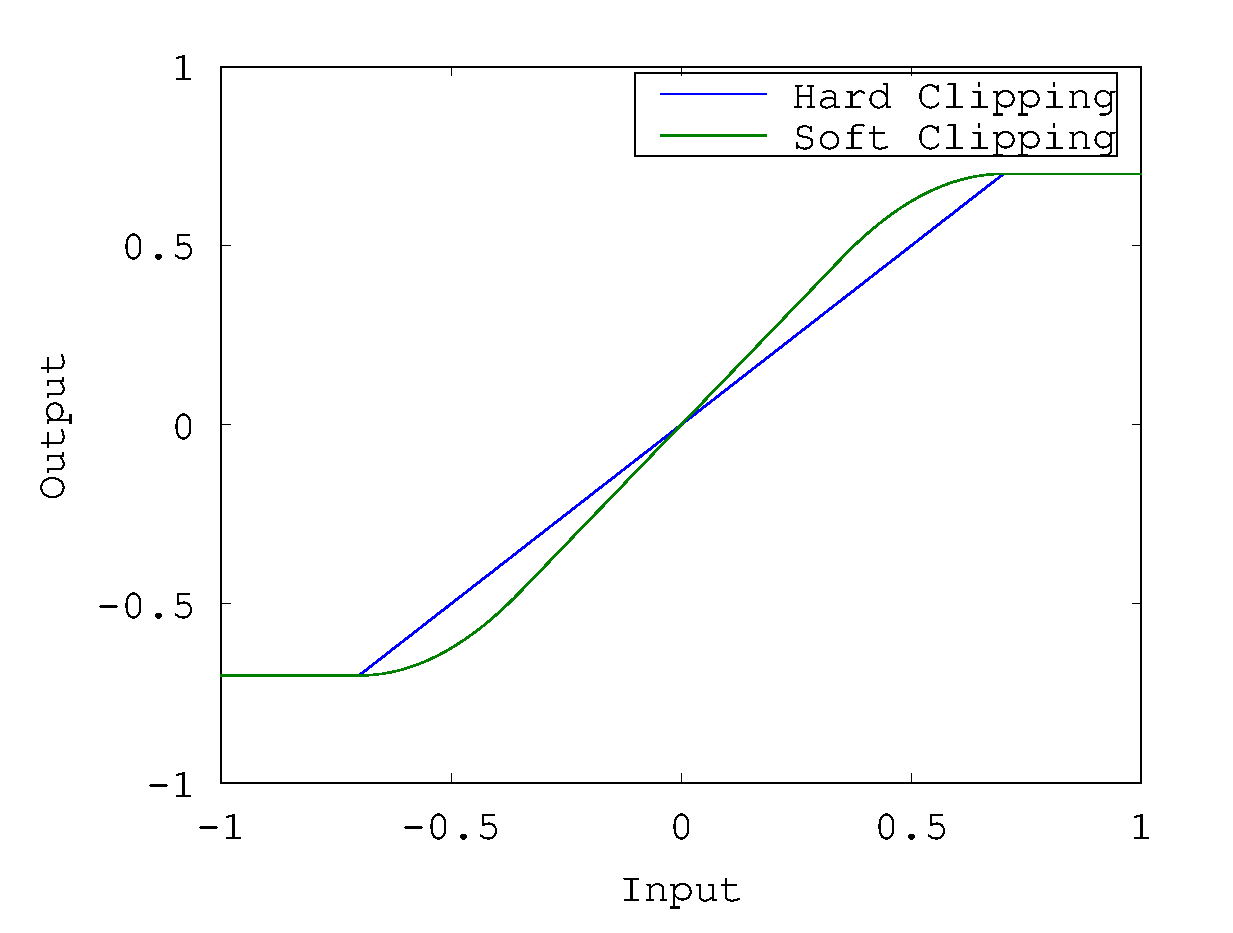
\includegraphics[width=0.6\textwidth]{chapter3/Images/Clipping.eps}
			\caption{Characteristic curves for \ref{eq:SymmetricHardClipping} and
				 \ref{eq:SymmetricSoftClipping} with a threshold of 0.5.}
			\label{fig:Clipping}
		\end{figure}

		\subsubsection*{Complexity}
			Most static nonlinearities only involve a few simple operations for each sample of the input
			signal. The hard clipper from Equation \ref{eq:SymmetricHardClipping} involves only comparisons and
			assignments. A soft clipper could also involve some multiplication and addition.
			
			As each sample is processed individually these algorithms have linear complexity.

		\subsubsection*{Homogeneity}
			The homogeneity of a static nonlinearity depends on the nonlinear function used. For different
			input amplitudes the set of harmonics generated by a given static nonlinearity will change. The
			ways in which this set of harmonics changes was investigated by \citet{enderby2012harmonic}.

			In that study the effects of several soft clippers on sinusoidal inputs were analysed. The levels
			of individual harmonics are plotted as a function of input amplitude. Figures
			\ref{fig:HardClippingHarmonics} and \ref{fig:SoftClippingHarmonics} show these plots for the
			clipping functions described previously.

			\begin{figure}[h!]
				\centering
				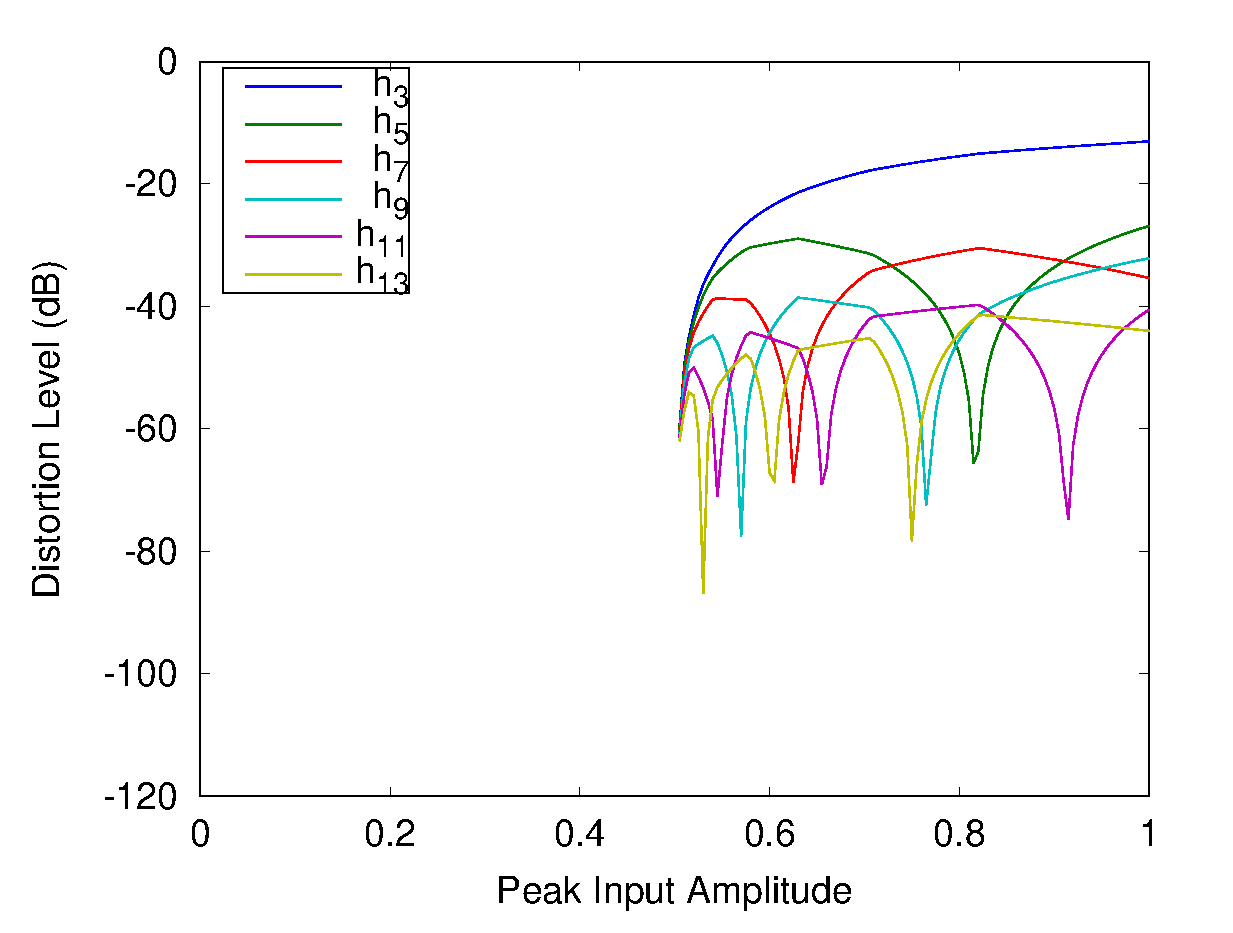
\includegraphics[width=0.6\textwidth]{chapter3/Images/HardClippingHarmonics.eps}
				\caption{Individual harmonic distortion levels for Equation \ref{eq:SymmetricHardClipping}
					 with a threshold of 0.5.}
				\label{fig:HardClippingHarmonics}
			\end{figure}

			\begin{figure}[h!]
				\centering
				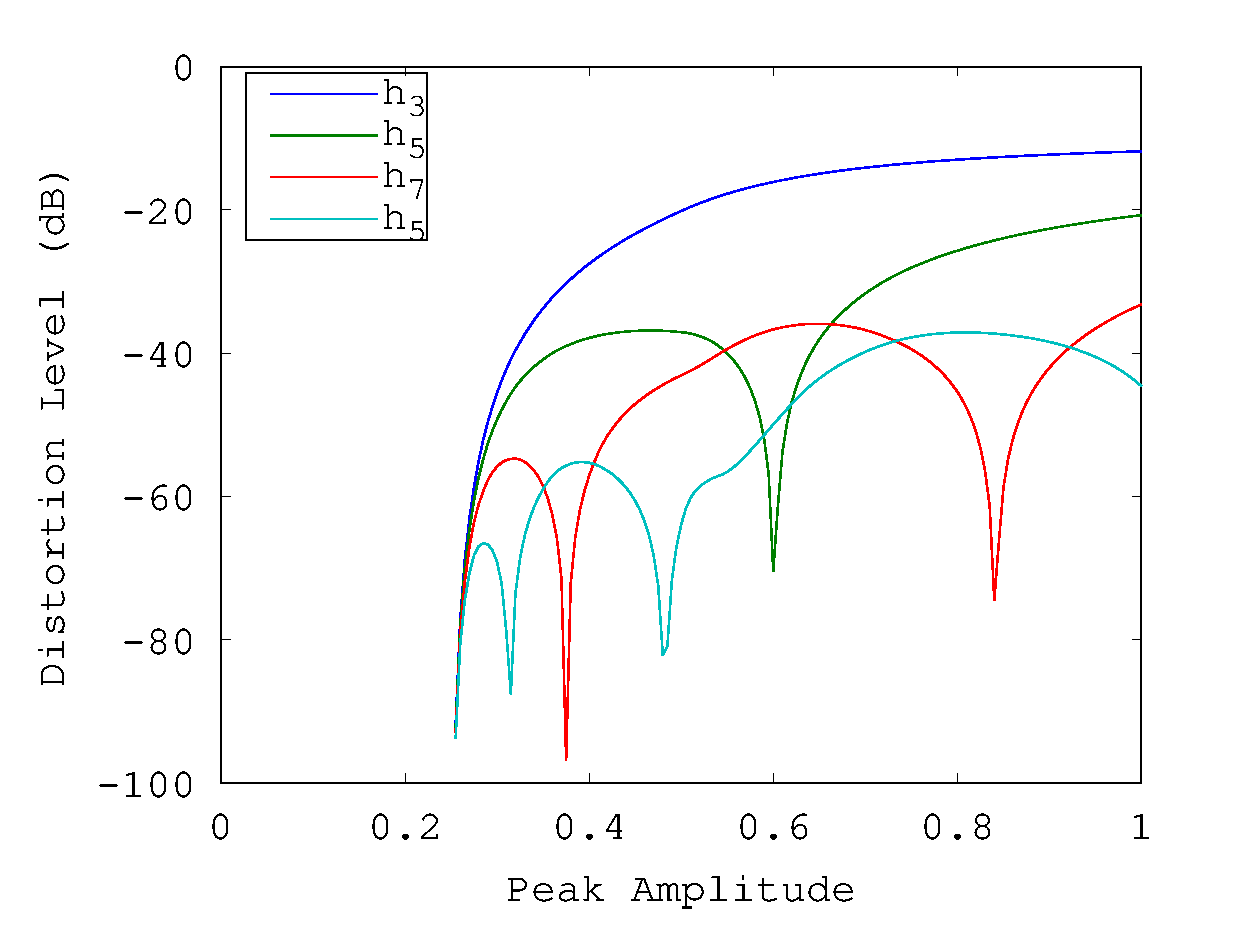
\includegraphics[width=0.6\textwidth]{chapter3/Images/SoftClippingHarmonics.eps}
				\caption{Individual harmonic distortion levels for Equation \ref{eq:SymmetricSoftClipping}
					 with a threshold of 0.5.}
				\label{fig:SoftClippingHarmonics}
			\end{figure}

			The first thing to note is that new harmonic components are only introduced once the input
			amplitude extends out of the linear section of the characteristic curve. Once input amplitude
			reaches a sufficient level harmonics are introduced but their amplitudes all vary independently.

			This behaviour can be improved on through the use of a different clipping function. Equation
			\ref{eq:SymmetricExponentialClipping} shows a function used to apply exponential clipping to a
			signal.
			
			\begin{equation}
				y(n) = \begin{cases}
					t\sgn(x(n)) & \text{if $|x(n)| > t$} \\
					t\sgn(x(n)) \left(1 - \left|\frac{x(n)}{t} - \sgn(x(n)) \right|^{E} \right) &
						\text{otherwise}
				\end{cases}, \quad t \geq 0 \ \text{and} \ E > 1
				\label{eq:SymmetricExponentialClipping}
			\end{equation}

			Where $E$ is a second parameter called the exponent. One advantage of this clipper is that it has
			no linear section. This means that harmonics are generated for input signals of any amplitude.
			Another advantage is that the levels of the generated harmonics vary more uniformly with input
			amplitude as shown in Figure \ref{fig:ExponentialClippingHarmonics}.

			\begin{figure}[h!]
				\centering
				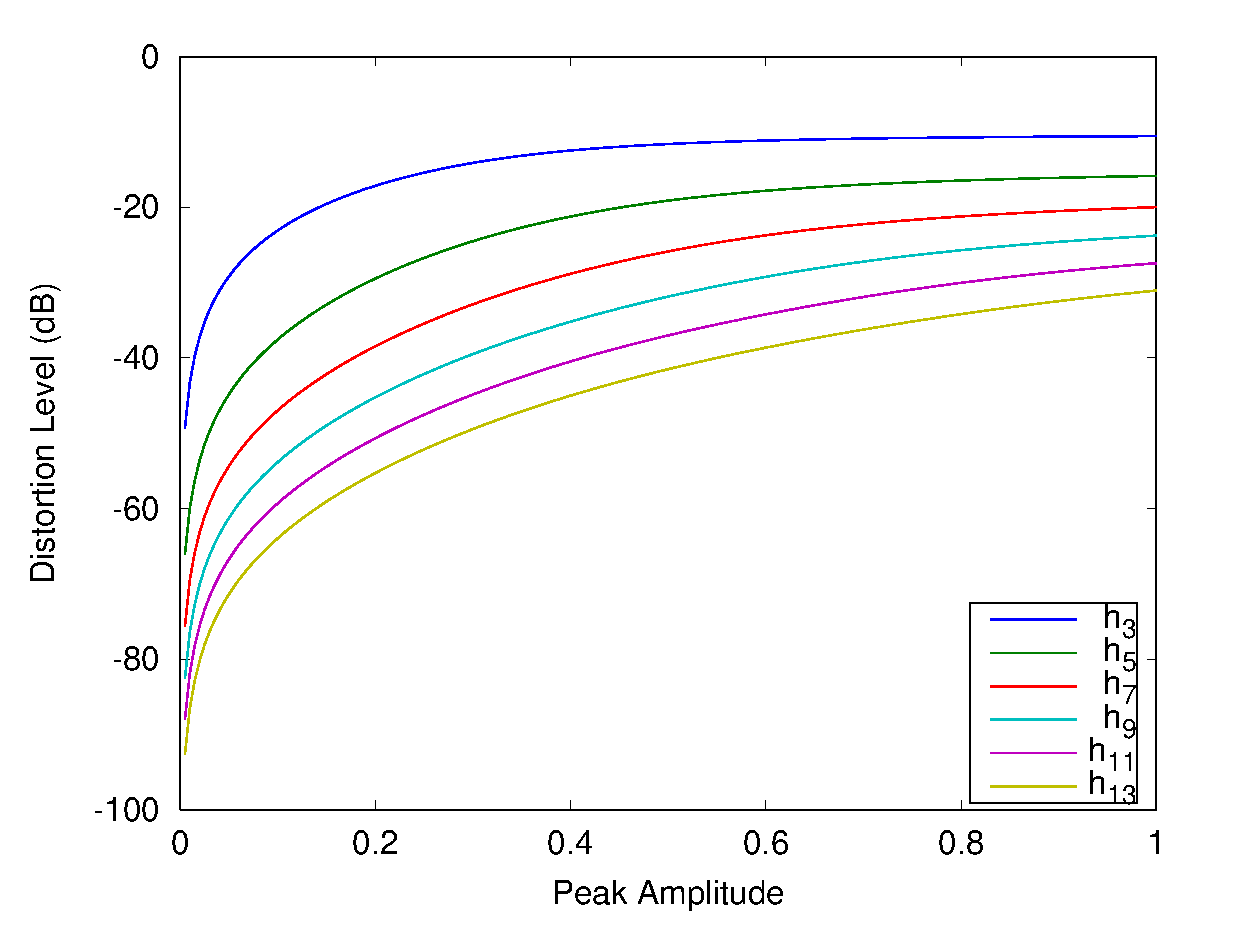
\includegraphics[width=0.6\textwidth]{chapter3/Images/ExponentialClippingHarmonics.eps}
				\caption{Individual harmonic distortion levels for Equation
					 \ref{eq:SymmetricExponentialClipping} with a threshold of 0.5 and an 
				         exponent of 5.}
				\label{fig:ExponentialClippingHarmonics}
			\end{figure}

			The non-homogeneity of simple clipping systems can be counteracted by introducing gain stages either
			side of the clipping stage. The first gain stage scales the signal so that the clipping stage will
			always clip the same proportion of the signal. The second gain stage scales the signal back to the
			original input amplitude. Analogously the clipping function can be scaled so as to always clip the
			same proportion of the signal, as done by \citet{deman2014adaptive}.

		\subsubsection*{Spectral Characteristics}
			The spectral characteristics depend on the function applied to the signal. If an odd function is
			used only odd order intermodulation components will be produced. Using an even function only even
			order components are generated. 

			The symmetric clippers discussed previously all use odd functions. It is evident from the harmonic
			amplitude plots that only odd order harmonics have been introduced to the signal. In order to
			generate even order harmonics these clipping function needs to be made asymmetric. This is easily
			done by clipping negative and positive portions of the input signal at different thresholds.
			Equation \ref{eq:SymmetricHardClipping} can be modified to allow for asymmetric clipping giving
			Equation \ref{eq:AsymmetricHardClipping}.
			
			\begin{equation}
				y(n) = \begin{cases}
					t_{+} & \text{if $x(n) > t_{+}$} \\
					t_{-} & \text{if $x(n) < t_{-}$} \\
					x(n) & \text{otherwise}
				\end{cases}, \quad t_{-} < t_{+}
				\label{eq:AsymmetricHardClipping}
			\end{equation}

			Where $t_{+}$ and $t_{-}$ are the clipping thresholds for positive and negative portions of the
			signal respectively.	

			The amplitudes of the generated harmonics will roll off at differing rates depending on the
			properties of the output signal. The spectrum will roll off at $6(n+1)$dB per octave when the
			$n^{\text{th}}$ derivative of the output signal is discontinuous \citep{kraght2000aliasing}.

			Hard clippers introduce discontinuities to the first derivative of a signal and so will introduce
			harmonics whose amplitudes will roll off at 12dB per octave. Signals clipped by Equation
			\ref{eq:SymmetricSoftClipping} are continuous in the first derivative \todo{(check this)} and so
			produce harmonics which roll off at a faster rate. This can be seen in Figure
			\ref{fig:ClippingSpectra}.

			\begin{figure}[h!]
				\centering
				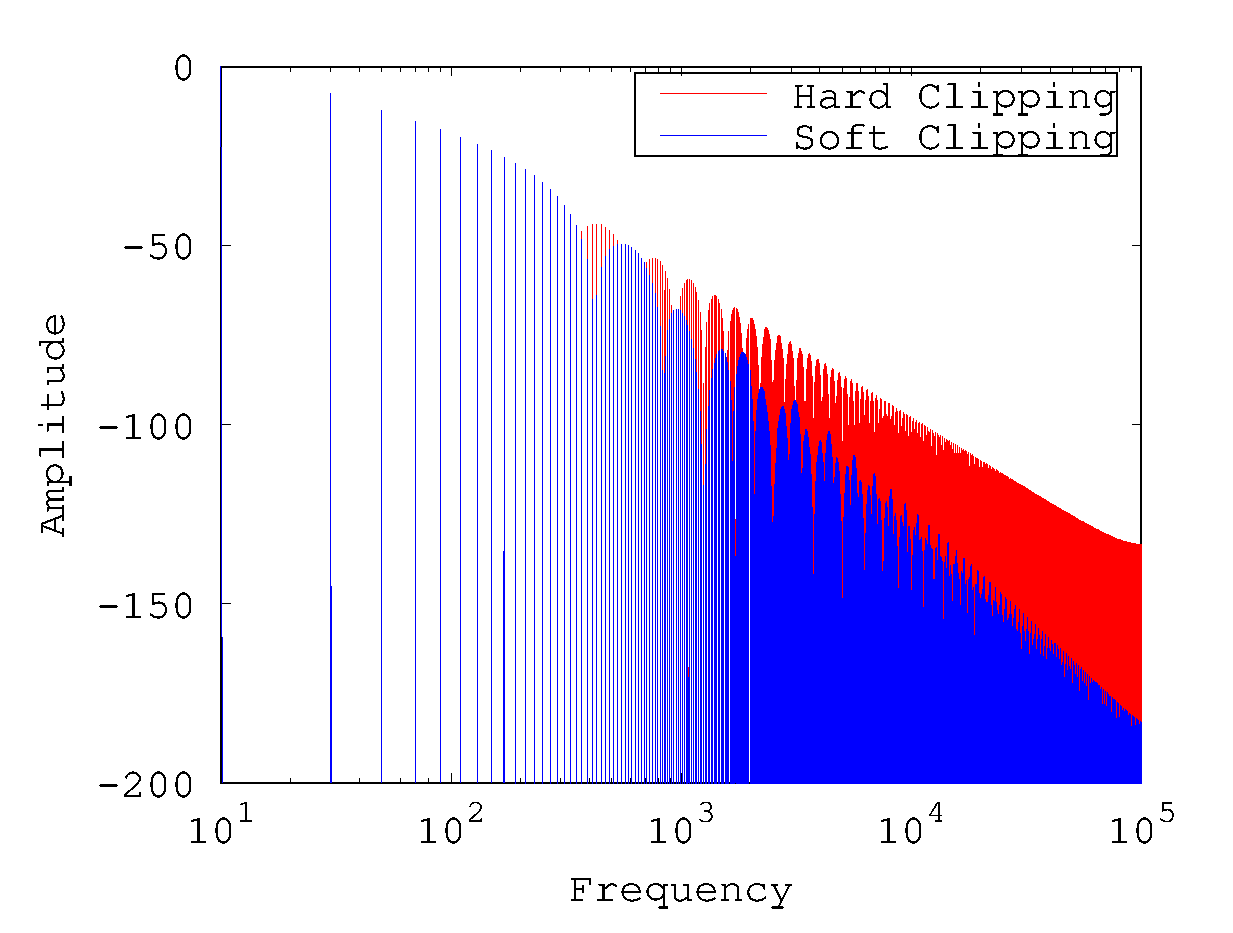
\includegraphics[width=0.6\textwidth]{chapter3/Images/ClippingSpectra.eps}
				\caption{Spectra of sinusoids clipped using Equations \ref{eq:SymmetricHardClipping} and
			                 \ref{eq:SymmetricSoftClipping}.}
				\label{fig:ClippingSpectra}
			\end{figure}

			The steeper roll off produced by soft clippers reduces the number of aliased frequencies produced.
			This is advantageous as aliased frequencies tend to be inharmonic.

		\subsubsection*{Temporal Characteristics}
		\subsubsection*{Preservation of Harmonicity}
		\subsubsection*{Flexibility}
		\subsubsection*{Naturalness}

	\subsection{Rectification}
	\label{sec:Excitation-Rectification}
		Rectification is a special case of static nonlinearity. Signals can be either half or full wave rectified,
		as shown in Equations \ref{eq:HalfWaveRectification} and \ref{eq:FullWaveRectification} respectively.

		\begin{equation}
			y(n) = \begin{cases}
				0 & \text{if $x(n) < 0$} \\
				x(n) & \text{otherwise}
			\end{cases}
			\label{eq:HalfWaveRectification}
		\end{equation}

		\begin{equation}
			y(n) = |x(n)|
			\label{eq:FullWaveRectification}
		\end{equation}

		\subsubsection*{Complexity}
		\subsubsection*{Homogeneity}
		\subsubsection*{Spectral Characteristics}
		\subsubsection*{Temporal Characteristics}
		\subsubsection*{Preservation of Harmonicity}
		\subsubsection*{Flexibility}
		\subsubsection*{Naturalness}

	\subsection{Integrator}
	\label{sec:Excitation-Integrator}
		Equation \ref{eq:Integrator} shows an Integrator adapted from the one described by \citet{larsen2004audio}.

		\begin{equation}
			y(n) = \begin{cases}
				0 & \text{if $x(n) > 0$ and $x(n - 1) \leq 0$} \\
				y(n - 1) + c|x(n)| & \text{otherwise}
			\end{cases}
			\label{eq:Integrator}
		\end{equation}

		\subsubsection*{Complexity}
		\subsubsection*{Homogeneity}
		\subsubsection*{Spectral Characteristics}
		\subsubsection*{Temporal Characteristics}
		\subsubsection*{Preservation of Harmonicity}
		\subsubsection*{Flexibility}
		\subsubsection*{Naturalness}

	\subsection{Multiplier}
	\label{sec:Excitation-Multiplier}
		\begin{equation}
			y(n) = x(n)^{h}, \quad h \in \mathbb{N}
			\label{eq:Multiplier}
		\end{equation}

		\subsubsection*{Complexity}
		\subsubsection*{Homogeneity}
		\subsubsection*{Spectral Characteristics}
		\subsubsection*{Temporal Characteristics}
		\subsubsection*{Preservation of Harmonicity}
		\subsubsection*{Flexibility}
		\subsubsection*{Naturalness}

	\subsection{Single Side Band Automodulation}
	\label{sec:Excitation-SSB}
		Single sideband automodulation utilises the concept of single sideband modulation
		\citep{corinthios2009signals}. This allows you to apply amplitude modulation to a signal and only produce
		either the sum or difference sideband.

		A simple way to apply single sideband modulation to a signal is through construction of an analytic signal.
		An analytic signal is a complex valued signal, the real part of which is the original signal and the
		imaginary part its Hilbert transform. The analytic signal is often denoted with a subscript letter
		$a$, such that the analytic representation of the signal $x(n)$ would be denoted $x_{a}(n)$.

		\note
		{
			We probably need some place to talk about hilbert transforms \citet{oppenheim2014discrete} are
			pretty good at that shiz.
		}

		In single sideband automodulation the analytical representation of the input signal is multiplied with
		itself in order to generate harmonics. Equation \ref{eq:SSB} shows the $h^{\text{th}}$ order single side
		band automodulation of a signal.

		\begin{equation}
			y(n) = \Re \left( x_{a}(n)^{h} \right), \quad h \in \mathbb{N}
			\label{eq:SSB}
		\end{equation}

		\subsubsection*{Complexity}
		\subsubsection*{Homogeneity}
		\subsubsection*{Spectral Characteristics}
		\subsubsection*{Temporal Characteristics}
		\subsubsection*{Preservation of Harmonicity}
		\subsubsection*{Flexibility}
		\subsubsection*{Naturalness}

	\subsection{Instantaneous Amplitude and Phase}
	\label{sec:Excitation-IAP}
		In this method, the instantaneous amplitude and phase of the analytic signal are calculated. These values
		are then used to aid in the construction of harmonics. The instantaneous amplitude of the analytic signal
		is found by taking its absolute value, $|x_{a}(n)|$. The instantaneous phase is found by taking the complex
		argument of the analytic signal, $\arg(x_{a}(n))$. The instantaneous phase can then be scaled in order to
		scale the frequency content of the signal independent of its amplitude. Equation \ref{eq:IAP} shows the
		$h^{\text{th}}$ order instantaneous amplitude and phase modulation of a signal.

		\begin{equation}
			y(n) = |x_{a}(n)| \cos \left( h\arg(x_{a}(n)) \right), \quad h \in \mathbb{N}
			\label{eq:IAP}
		\end{equation}

		\subsubsection*{Complexity}
		\subsubsection*{Homogeneity}
		\subsubsection*{Spectral Characteristics}
		\subsubsection*{Temporal Characteristics}
		\subsubsection*{Preservation of Harmonicity}
		\subsubsection*{Flexibility}
		\subsubsection*{Naturalness}

	\subsection{Spectral Replication}
	\label{sec:Excitation-SpectralReplication}
		The principle behind spectral replication is to reproduce the spectral structure of a signal at higher
		frequencies.

		\begin{figure}[h!]
			\centering
			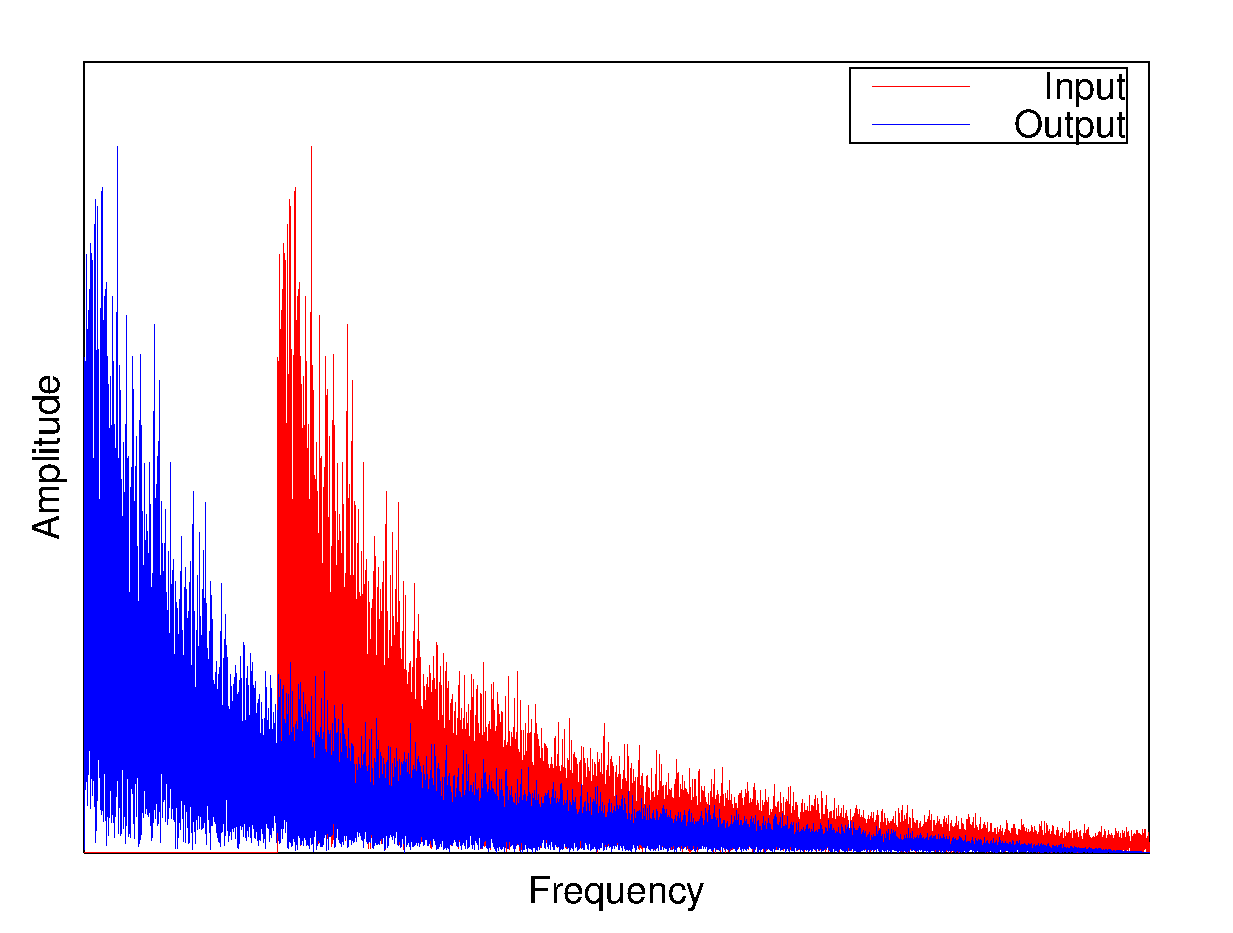
\includegraphics[width=0.6\textwidth]{chapter3/Images/SpectralReplicationSpectrum.eps}
			\caption{The spectral characteristics of spectral replication.}
			\label{fig:SpectralReplication}
		\end{figure}

		This spectral shift is easily implemented through the use of single side band modulation as shown in
		Equation \ref{eq:SpectralReplication}.

		\begin{equation}
			y(n) = \Re \left( x_{a}(n) e^{j\omega  n/ f_{s}} \right)
			\label{eq:SpectralReplication}
		\end{equation}

		Where $\omega$ is the angular frequency the signal should be shifted by and $f_{s}$ is the sampling
		frequency of the signal.

		\subsubsection*{Complexity}
		\subsubsection*{Homogeneity}
		\subsubsection*{Spectral Characteristics}
		\subsubsection*{Temporal Characteristics}
		\subsubsection*{Preservation of Harmonicity}
		\subsubsection*{Flexibility}
		\subsubsection*{Naturalness}

	\subsection{Spectral Folding}
	\label{sec:Excitation-SpectralFolding}
	
		\begin{figure}[h!]
			\centering
			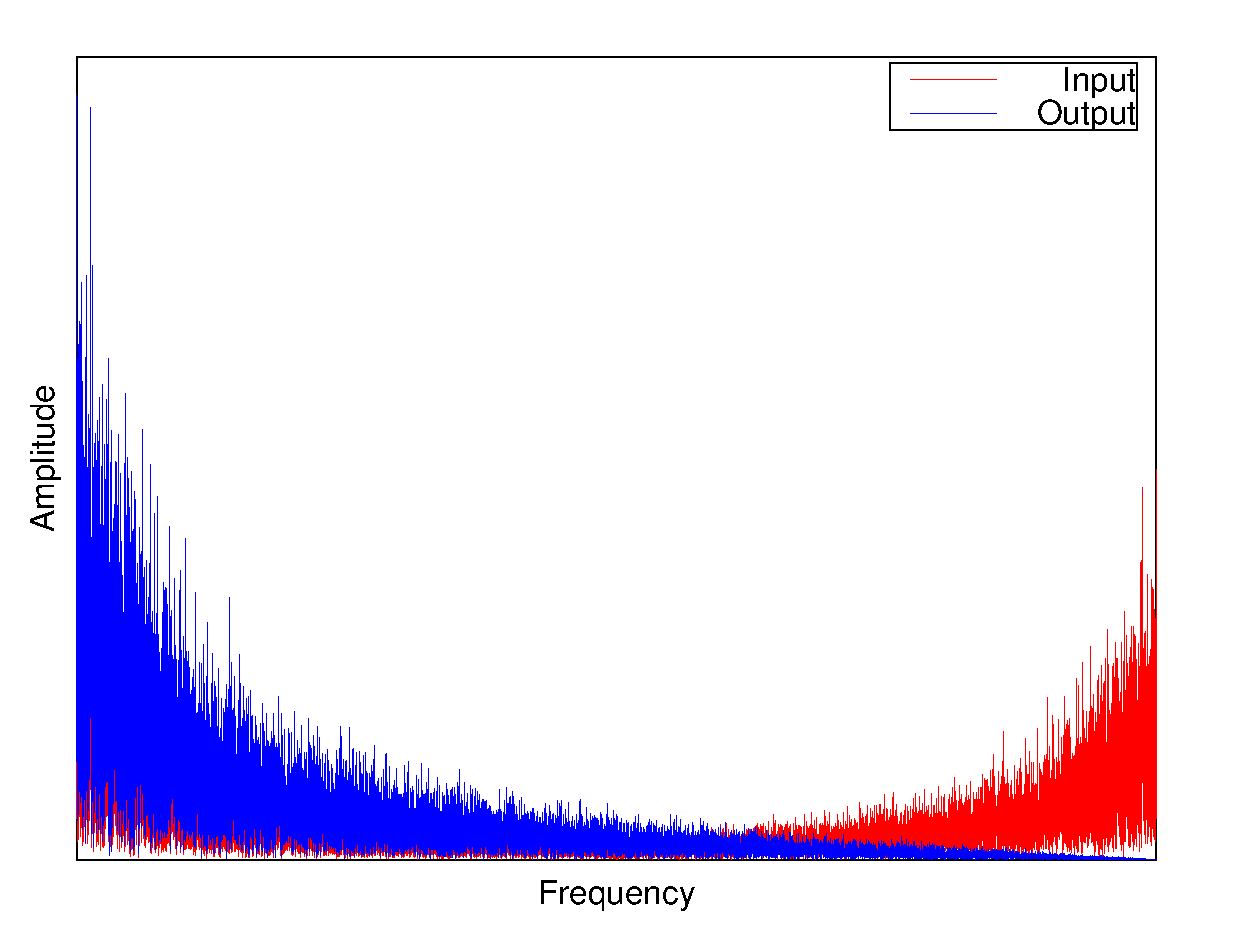
\includegraphics[width=0.6\textwidth]{chapter3/Images/SpectralFoldingSpectrum.eps}
			\caption{The spectral characteristics of spectral folding.}
			\label{fig:SpectralFolding}
		\end{figure}

		\begin{equation}
			y(n) = \begin{cases}
				-x(n) & \text{if $n$ is odd} \\
				x(n) & \text{otherwise}
			\end{cases}
			\label{eq:SpectralFolding}
		\end{equation}

		\subsubsection*{Complexity}
		\subsubsection*{Homogeneity}
		\subsubsection*{Spectral Characteristics}
		\subsubsection*{Temporal Characteristics}
		\subsubsection*{Preservation of Harmonicity}
		\subsubsection*{Flexibility}
		\subsubsection*{Naturalness}

	\subsection{Spectral Stretching}
	\label{sec:Excitation-SpectralStretching}

		\begin{figure}[h!]
			\centering
			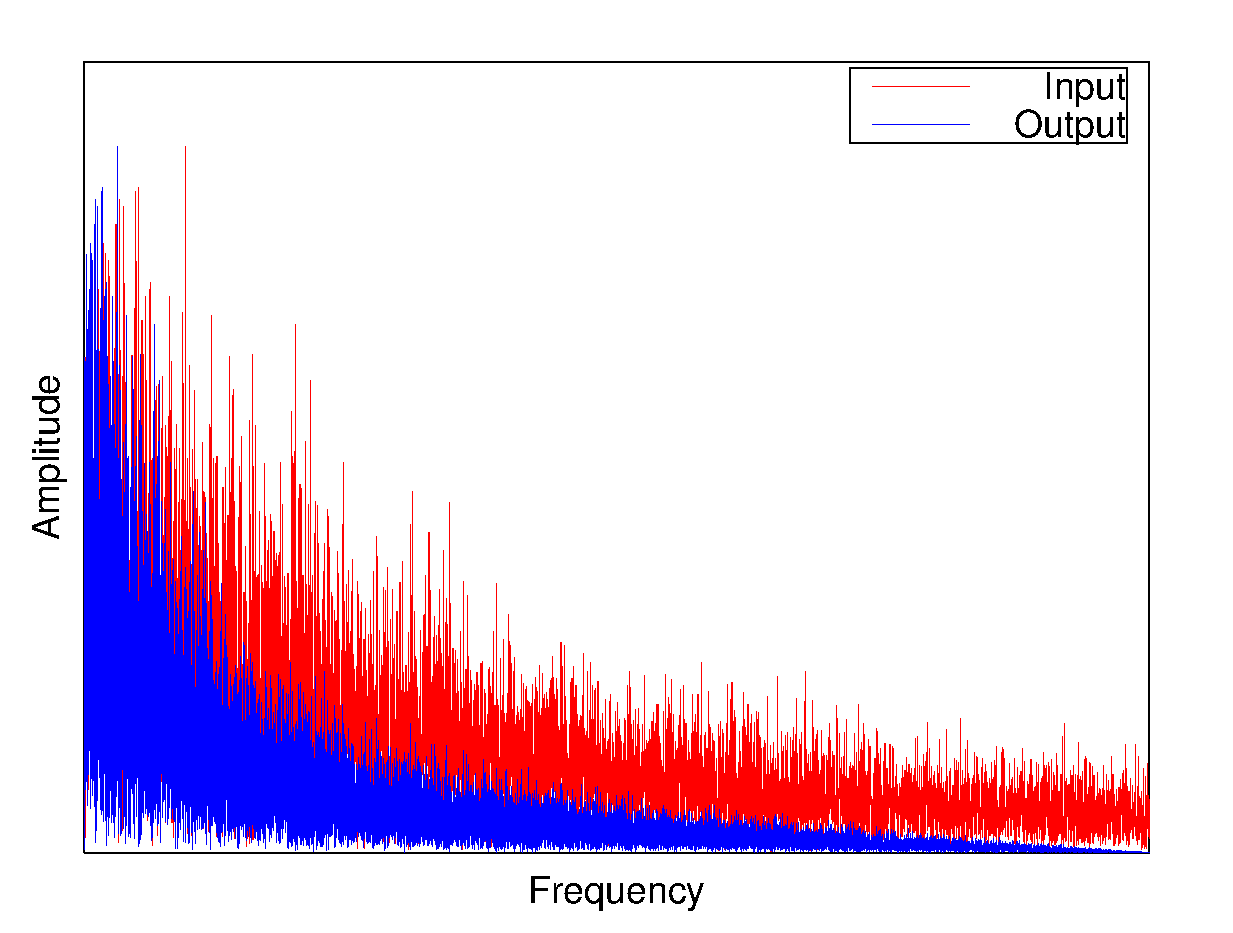
\includegraphics[width=0.6\textwidth]{chapter3/Images/SpectralStretchingSpectrum.eps}
			\caption{The spectral characteristics of spectral stretching.}
			\label{fig:SpectralStretching}
		\end{figure}

		\subsubsection*{Complexity}
		\subsubsection*{Homogeneity}
		\subsubsection*{Spectral Characteristics}
		\subsubsection*{Temporal Characteristics}
		\subsubsection*{Preservation of Harmonicity}
		\subsubsection*{Flexibility}
		\subsubsection*{Naturalness}

	%\subsection{Bandwidth Extension}
	%\label{sec:Excitation-BWE}
	%	\note
	%	{
	%		A nice summary in \citet{larsen2004audio}.

	%		Look at Figure \ref{fig:SpectralFolding} 'aint it fancy.
	%	}

	%	\begin{figure}[h!]
	%		\centering
	%		\subfloat[Spectral Folding]
	%		{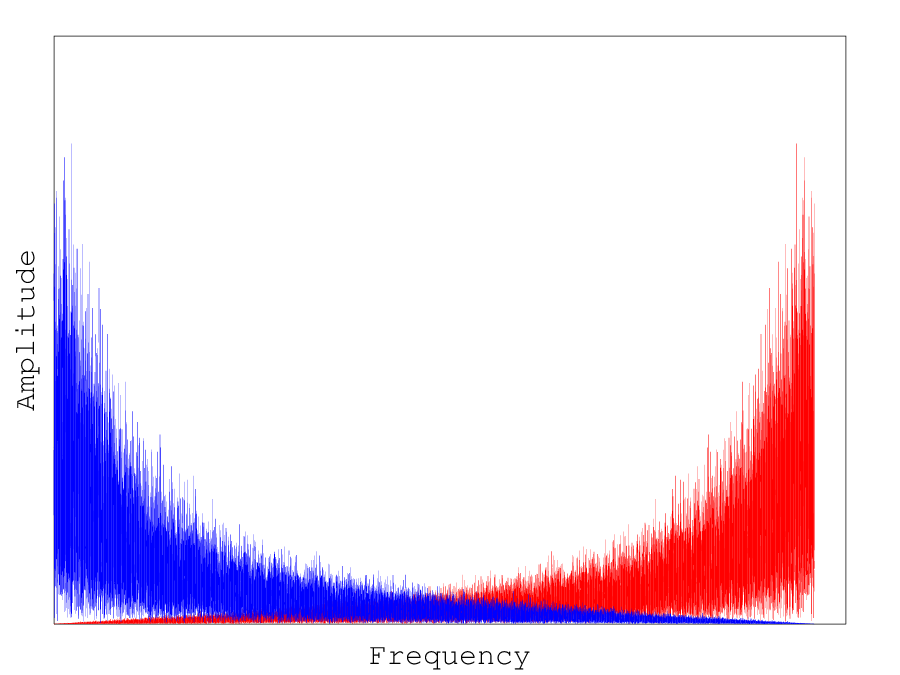
\includegraphics[width=0.4\textwidth]{chapter3/Images/SpectralFolding.png}}
	%		\subfloat[Spectral Replication]
	%		{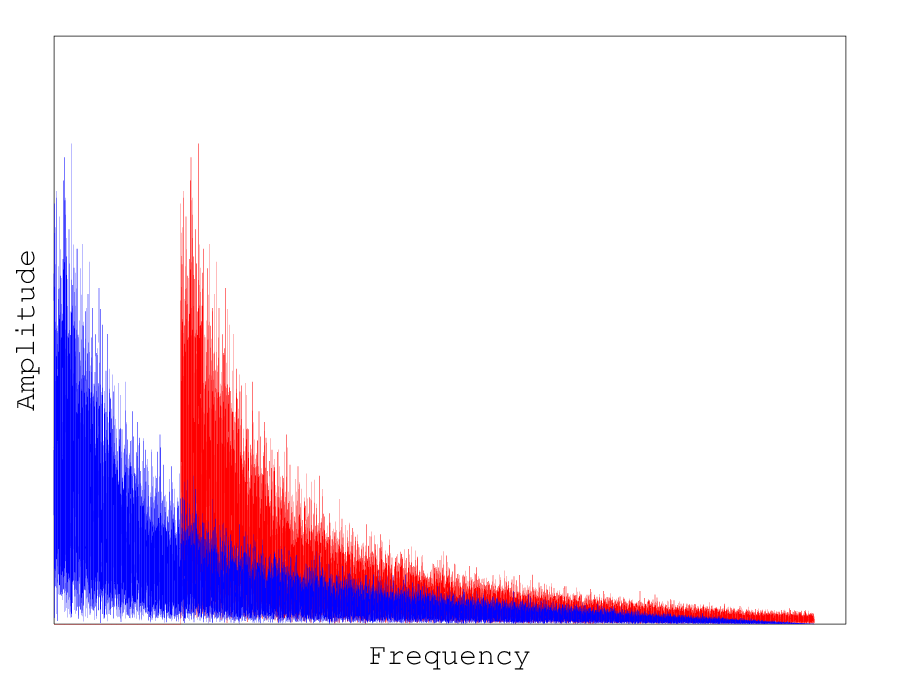
\includegraphics[width=0.4\textwidth]{chapter3/Images/SpectralReplication.png}}
	%		\\
	%		\subfloat[Spectral Stretching]
	%		{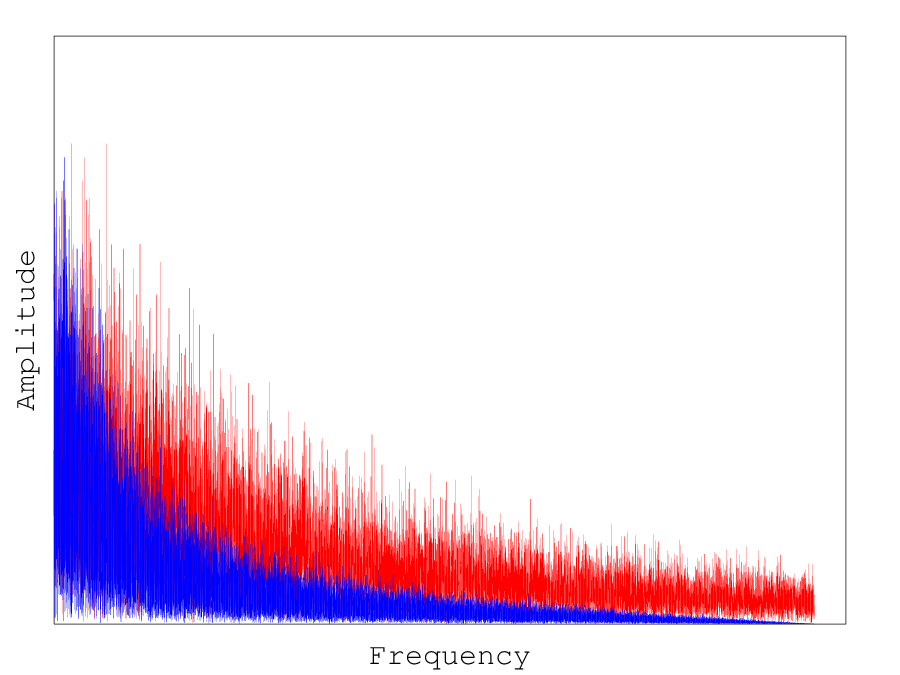
\includegraphics[width=0.4\textwidth]{chapter3/Images/SpectralStretching.png}}
	%		\caption{Spectral characteristics of different band width extension methods. In each graph the blue 
	%		section represents the original spectra and the red section the new spectral content.}
	%		\label{fig:SpectralFolding}
	%	\end{figure}

	\subsection{Individual Harmonic Generation}
	\label{sec:Excitation-Individuals}
		\note{SMC paper}

	\subsection{Psychoacoustic Enhancers}
	\label{sec:Excitation-Enhancers}
		\note
		{
			Probably the most well known perceptual control effects out there. The Aural Exciter has been 
			covered by both \citet{chalupper2000aural} and \citet{shekar2013modeling}.
		}

	\subsection{Fundamental Frequency Tracking}
	\label{sec:Excitation-Fundamental}
		\note
		{
			Several generation methods can be improved through tracking the fundamental frequency of the input 
			signal.

			We can talk all about fundamental / pitch tracking here \citep{cuadra2001efficient, 
			gerhard2003pitch, prukkanon2009vt-amdf, larsen2004audio}.
		}

\begin{landscape}
\section{Methods Comparison}
\label{sec:Excitation-Comparison}

	\begin{tabular}{|c|c|c|c|c|c|c|}
		\hline
		\bf{Method} & \bf{Complexity} & \bf{Homogeneity} & \bf{Spectral Properties} & \bf{Temporal Properties} & \bf{IMD}
		\bf{Flexibility} & \bf{Naturalness} \\
		\hline
		Static Nonlinearity & $\mathcal{O}(n)$ & & & & & \\
		\hline
		Rectifier & $\mathcal{O}(n)$ & & & & & \\
		\hline
		Integrator & $\mathcal{O}(n)$ & & & & & \\
		\hline
		Multiplier & $\mathcal{O}(n)$ & & & & & \\
		\hline
		SSB & $\mathcal{O}(n)$ & & & & & \\
		\hline
		IAP & $\mathcal{O}(n)$ & & & & & \\
		\hline
		Spectral Replicator & $\mathcal{O}(n)$ & & & & & \\
		\hline
		Spectral Mirror & $\mathcal{O}(n)$ & & & & & \\
		\hline
		Spectral Stretch & $\mathcal{O}(n\log{n})$ Assuming FFT used & & & & & \\
		\hline
	\end{tabular}

\end{landscape}

%\section{Evaluating Excitation Methods}
%\label{sec:FeatureControl-MethodEvaluation}
%
%	\note{Homogeneity a la DAFx paper.
%	      Flexibility introduced by allowing single harmonic control a la SMC paper}
%
%	Several harmonic excitation methods were discussed in Section \ref{sec:Excitation-Methods}. When applied to the 
%	task of controlling specific audio features each of these methods has its own advantages and disadvantages.
%
%	\subsection{Homogeneity}
%	\label{sec:FeatureControl-Homogeneity}
%
%		\subsubsection*{Static Nonlinearities}		
%			As previously mentioned simple static nonlinearities are very susceptible to change in input 
%			amplitude. \citet{deman2014adaptive} counteract this issue by having the clipping threshold adapt 
%			to changes in the RMS amplitude of the input. The user is then provided with a `relative threshold' 
%			parameter on which the same setting should give similar perceptual results no matter what the input 
%			amplitude.
%
%			\note{Talk about the issues with static nonlinearities raised in \citet{enderby2012harmonic}}
%
%		\subsubsection*{Bandwidth Extension}
%			\note{Spectral mirroring, stretching and replication are all homogeneous.}
%			
%		\subsubsection*{Single Harmonic Generation}
%			Using single sideband automodulation the proportion of new frequency components in the output 
%			signal increases as the input amplitude increases. The instantaneous amplitude and phase and phase 
%			vocoder techniques are more robust in this respect.
%
%	\subsection{Flexibility}
%	\label{sec:FeatureControl-Flexibility}
%
%		\note{Flexibility is provided by individual harmonic generation \citep{enderby2013methods}}	
%
%	\subsection{Complexity}
%	\label{sec:FeatureControl-Complexity}
%		
%		\note{It is advantageous to use an algorithm that will create accurate harmonics with little analysis.
%		      Most methods don't rely on knowing the fundamental in order to generate harmonics. Spectral
%		      shifting on the other hand does.}
%
%		\note{Most of the algorithms can be easily improved through the use of a low pass filter, increasing
%	             complexity.}

\chapter{Subjective Timbre Evaluation}
\label{chap:TimbreEvaluation}
	\todo{Come up with a better name for this chapter.}

\section{Introduction}
\label{sec:TimbreEvaluation-Introduction}
	In order to manipulate the perceptual characteristics of a sound it is necessary to know the relationships between
	low level audio features and semantic descriptions. In Chapter \ref{chap:Timbre} several different methods for
	obtaining this information were discussed.  In this chapter a new method of collecting semantically annotated audio
	feature data is presented (Section \ref{sec:TimbreEvaluation-DAWBasedTimbreEvaluation}). Data gathered using this
	method is then analysed, producing a list of semantic descriptors and the low level audio features which contribute
	to them (Section \ref{sec:TimbreEvaluation-Analysis}).

\section{Production Environment Timbre Evaluation} % this name will probably change
\label{sec:TimbreEvaluation-DAWBasedTimbreEvaluation}
	The perceptual listening test methodologies discussed in Section \ref{sec:Timbre-ListeningTests} rely on the
	participants performing a certain set of tasks. While this structure helps to reduce the number of variables in an
	experiment, it does not necessarily reflect the way audio is treated in a production environment.

	A new methodology has been developed in which the analysis of timbre is introduced into a typical music production
	workflow, causing minimal interruption to the producer. This methodology aims to answer the question "What terms do
	music producers use to describe the timbral transforms, they apply to audio, during the creation of music?". 

	This section will detail a typical production workflow is and how semantic information can be gathered.

	\subsection{Music Production Workflow}
	\label{sec:TimbreEvaluation-DAWBasedTimbreEvaluation-Workflow}
		\todo{Find some references for this section. Probably mixing engineers handbook or something.}

		The music production workflow has four main stages:

		\begin{itemize}
			\item Recording
			\item Editing
			\item Mixing
			\item Mastering
		\end{itemize}

		At every stage of this process semantic descriptors are often used to communicate the desired timbral
		qualities of the audio. For instance, one my ask that a certain microphone be used because of the `warmth'
		it adds to the recorded sound. During the mixing and mastering stages audio processing effects are applied
		to shape the timbre further. These stages will be the focus of this section as the aim of this thesis is
		to improve the intuitiveness of these effects.

		Historically, audio production required the use of several pieces of electronic hardware, including
		microphones, a mixing console, audio processing effects and a recording device. Modern music production
		techniques utilise Digital Audio Workstation (DAW) software. This software performs the tasks of many
		pieces of hardware, enabling users to record, edit and mix multiple tracks of audio using a computer. 
		
	\subsection{Analysis of Timbre Inside the DAW}
	\label{sec:TimbreEvaluation-DAWBasedTimbreEvaluation-InDAW}
		An ideal way to collect timbral information during music production would be to have the DAW analyse the
		audio tracks used and production techniques applied. Information which could be gathered directly from the
		DAW, with no extra input from the user, includes:

		\begin{itemize}
			\item Information about the audio processing chain:
			\begin{itemize}
				\item The effects applied to each track.
				\item The order in which these effects are applied.
				\item The parameter settings of these effects.
			\end{itemize}
			\item Features of the audio signal at every stage in the processing chain.
		\end{itemize}

		Additional information can be gathered by prompting the user for input:

		\begin{itemize}
			\item The genre of music being produced.
			\item The content of the separate audio tracks (what instruments etc.).
			\item Semantic terms which describe the timbral transforms applied by each audio
			      effect.
		\end{itemize}

		Achieving this would require the creation of a new DAW. This would be impractical for the current research.
		DAWs are comprehensive software packages which perform many more tasks than the application of audio
		effects (project management, audio editing functionality etc.). A lot of effort would be expended in
		implementing these features before any timbral data could be collected. Music producers also tend to have
		a preferred DAW with which they work most fluidly. Convincing producers to use a new DAW, for the purposes
		of research, would be a difficult task.

		Third party developers can produce extensions to DAWs known as plug-ins. Plug-Ins provide additional audio
		processing functionality to the DAW environment. They can optionally expose their own parameters which
		users can adjust to achieve their desired effect. There are several different formats in which audio
		plug-ins can be distributed (VST, AU etc.). Most of the commonly used DAWs support plug-ins in one or more
		of these formats.

		Audio plug-ins provide a good platform to allow producers to provide semantic terms and audio feature
		information from within their preferred DAW. As part of this research a suite of audio plug-ins which
		extract this information have been developed. They have been released under the title Semantic Audio
		Feature Extraction (SAFE) Plug-Ins.

	\subsection{SAFE Plug-Ins}
	\label{sec:TimbreEvaluation-DAWBasedTimbreEvaluation-SAFE}
		The SAFE plug-ins consist of four commonly used audio effects: Equaliser, Distortion, Compressor and
		Reverb. As part of the plug-ins's interface, the user has the option to save semantic terms. The interface
		for the SAFE Distortion is shown in Figure \ref{fig:SAFE-Distortion}. Upon saving terms the plug-in will
		analyse the audio at its inputs and outputs. When the analysis is completed the results are stored,
		containing:

		\begin{itemize}
			\item The users semantic description of the transform.
			\item The plug-in's current parameter settings.
			\item The features of the audio before and after processing.
			\item Some additional data about the user and the track being worked on.
			\begin{itemize}
				\item The genre.
				\item The instrument.
				\item The users age.
				\item The users location.
				\item The users primary language.
				\item The number of year experience the user has in music production.
			\end{itemize}
		\end{itemize}

		\begin{figure}[h!]
			\centering
			\includegraphics[width=0.8\textwidth]{chapter4/Images/SAFEDistortion.png}
			\caption{The interface for the SAFE distortion plug-in.}
			\label{fig:SAFE-Distortion}
		\end{figure}

		In total, the SAFE plug-ins analyse five seconds of audio both before and after processing. The audio is
		analysed in frames of 4096 samples using the LibXtract software library \citep{bullock2007libxtract},
		calculating 80 different audio features for each frame. These features are split into five groups as
		follows:

		\begin{itemize}
			\item {\bf{Temporal Features:}} Features calculated from the temporal representation of the signal.
			\begin{itemize}
				\item Signal Mean ($\mu$), Signal Variance ($\sigma^{2}$), Signal Standard Deviation
				      ($\sigma$), RMS Amplitude ($\textrm{RMS}$) and Zero Crossing Rate ($\textrm{ZCR}$).
			\end{itemize}
			\item {\bf{Spectral Features:}} Features calculated from the DFT of the signal.
			\begin{itemize}
				\item Spectral Centroid ($\mu_{\textrm{s}}$), Spectral Spread ($\sigma_{\textrm{s}}^{2}$),
				      Spectral Standard Deviation ($\sigma_{\textrm{s}}^{2}$), Spectral Skewness
				      ($\gamma_{\textrm{s}}$), Spectral Kurtosis ($\kappa_{\textrm{s}}$), Jensen
				      Irregularity ($\textrm{JI}$), Krimphoff Irregularity ($\textrm{KI}$), $f_{0}$,
				      Spectral Smoothness ($\textrm{SSm}$), Spectral Roll Off ($\textrm{SRO}$), Spectral
				      Flatness ($\textrm{SF}$), Tonality ($\tau$), Spectral Crest ($\textrm{SC}$)
				      and Spectral Slope ($\textrm{SSl}$).
			\end{itemize}
			\item {\bf{Peak Spectral Features:}} Features calculated from the spectral partials of the signal.
			\begin{itemize}
				\item Peak Spectral Centroid ($\mu_{\textrm{p}}$), Peak Spectral Spread
				      ($\sigma_{\textrm{p}}^{2}$), Peak Spectral Standard Deviation
				      ($\sigma_{\textrm{p}}^{2}$), Peak Spectral Skewness ($\gamma_{\textrm{p}}$), Peak
				      Spectral Kurtosis ($\kappa_{\textrm{p}}$), Peak Jensen Irregularity
				      ($\textrm{JI}_{\textrm{p}}$), Peak Krimphoff Irregularity
				      ($\textrm{KI}_{\textrm{p}}$), Peak Tristimuli ($T_{\textrm{p}1}$, $T_{\textrm{p}2}$
				      and $T_{\textrm{p}3}$) and Inharmonicity ($I$).
			\end{itemize}
			\item {\bf{Harmonic Spectral Features:}} Features calculated from the harmonic partials of the
			      signal.
			\begin{itemize}
				\item Harmonic Spectral Centroid ($\mu_{\textrm{h}}$), Harmonic Spectral Spread
				      ($\sigma_{\textrm{h}}^{2}$), Harmonic Spectral Standard Deviation
				      ($\sigma_{\textrm{h}}$), Harmonic Spectral Skewness ($\gamma_{\textrm{h}}$), Harmonic
				      Spectral Kurtosis ($\kappa_{\textrm{h}}$), Harmonic Jensen Irregularity
				      ($\textrm{JI}_{\textrm{h}}$), Harmonic Krimphoff Irregularity
				      ($\textrm{KI}_{\textrm{h}}$), Tristimuli ($T_{1}$, $T_{2}$ and $T_{3}$), Noisiness
				      ($N$) and Odd to Even Harmonic Ratio ($\textrm{ROE}$).
			\end{itemize}
			\item {\bf{Bark Coefficients (}}$\textrm{Bark}_{0\textrm{-}24}${\bf{):}} The 25 bark band
			      coefficients.
			\item {\bf{MFCCs (}}$\textrm{MFCC}_{0\textrm{-}12}${\bf{):}} The 13 MFCCs.
		\end{itemize}

		One disadvantage in using plug-ins is that they cannot gather information about the processing chain they
		may be a part of. The timbral transform the user is describing may be the result of several effects working
		together. This can be mitigated somewhat by asking users to describe only the effect the plug-in in
		question is providing.

		The SAFE plug-ins suffer from the same issues other distributed tests do. The researcher forfeits control
		over the listening environment in order to gather results from a much larger sample of people. In fact they
		provide even lest control than methodologies like that used in the Social EQ project
		\citep{cartwright2013socialeq} in that the choice of audio samples being used is decided by the test
		subject. 

	\subsection{SAFE Ontology}
	\label{sec:TimbreEvaluation-DAWBasedTimbreEvaluation-SAFEOntology}
		\note{Really not sure how well this fits in here. Do we needs a section explaining RDF and such? Where
		would that go?}

		The data collected using the SAFE plug-ins is stored as RDF triples using the SAFE ontology.  The SAFE
		Ontology was designed to describe the semantics relating to the application of an audio effect and the
		statistical audio features of the signals involved. It acts as an extension to the Audio Effects Ontology
		\citep{wilmering2013the}, introducing additional concepts for the description of semantic data.  This
		additional data can be separated into three groups:

		\begin{itemize}
			\item Metadata describing the application of the effect.
			\item Audio feature data for the input and output signals.
			\item Provenance of the data.
		\end{itemize}

		Each entry in the SAFE dataset is described using the \emph{studio:Transform} concept, applying some
		semantic transform to a set of input signals to produce a set of output signals. The structure of this data
		is shown in Figure \ref{fig:TransformGraph}.

		\begin{figure}[h!]
			\centering
			\begin{tikzpicture}[->,>=stealth',node distance=3cm]
				\tikzstyle{object} = [style=ellipse]

				\node[object, fill=blue] (transform) {studio:Transform};
				\node[object, fill=green] (signal) [below left of=transform] {mo:Signal};
				\node[object, fill=orange] (descriptor) [above of=transform] {safe:DescriptorItem};
				\node[object, fill=orange] (metadata) [below right of=transform] {safe:MetadataItem};
				\node[object, fill=pink] (device) [above right=1.5cm and 0.8cm of transform] {afx:Device};
				\node[object, fill=pink] (state) [above left=1.5cm and 0.8cm of transform] {afx:State};
				\node[object, fill=gray] (harsh) [above=1cm of descriptor] {"Harsh"};

				\path (transform) edge [bend left] node [right, overlay] {prov:used} (signal)
				      edge [bend right] node [left, overlay] {prov:generated} (signal)
				      edge node [right, overlay] {safe:descriptor} (descriptor)
				      edge [bend left] node [right, overlay] {safe:metadata} (metadata)
				      edge [bend right] node [right, overlay] {studio:effect} (device)
				      edge [bend left] node [left, overlay] {afx:state} (state)
				      (signal) edge [bend right] node [below, overlay] {safe:metadata} (metadata)
				      (descriptor) edge node [right, overlay] {rdfs:comment} (harsh);
			\end{tikzpicture}
			\caption{The structure used to describe the application of an audio effect.}
			\label{fig:TransformGraph}
		\end{figure}

		Here, users provide a term, or series of terms, to describe the transform applied by the audio effect in
		its current state. This should describe the perceived difference between the output and input signals. In
		the SAFE Ontology this is modelled through the \emph{safe:DescriptorItem} concept which provides a semantic
		description for each transform. Metadata items are used to provide details about the application domain of
		the effect, where each metadata item describes one property of an object, the property being identified
		using an \emph{rdfs:label} and the description provided using an \emph{rdfs:comment}. Each object described
		by a metadata item has its own set of properties, ``genre'' and ``instrument'' metadata tags for example,
		describe an audio signal, while ``location'' metadata tags describe a transform.

		The analysis of audio signals is described using the concept \emph{safe:FeatureExtractionTransform},
		similar to a \emph{studio:Transform} but taking an audio signal as input and producing feature values at
		the output, as shown in Figure \ref{fig:ExtractionGraph}.

		\begin{figure}[h!]
			\centering
			\begin{tikzpicture}[->,>=stealth',node distance=3cm]
				\tikzstyle{object} = [style=ellipse]

				\node[object, fill=orange] (extraction) {safe:FeatureExtractionTransform};
				\node[object, fill=gray] (feature) [above of=extraction] {"Spectral Centroid"};
				\node[object, fill=gray] (frameSize) [above left of=extraction] {"4096"};
				\node[object, fill=gray] (stepSize) [above right of=extraction] {"1024"};
				\node[object, fill=green] (signal) [below left of=extraction] {mo:Signal};
				\node[object, fill=purple] (event) [below right of=extraction] {event:Event};
				\node[object, fill=yellow] (interval) [below=1cm of signal] {tl:Interval};
				\node[object, fill=yellow] (instant) [below=1cm of event] {tl:Instant};
				\node[object, fill=yellow] (timeline) [below right of=interval] {tl:TimeLine};
				\node[object, fill=gray] (value) [below right=0.2cm and 0.6cm of event] {"2543.4"};
				\node[object, fill=gray] (time) [below right=0.2cm and 0.6cm of instant] {"4048"};

				\path (extraction) edge [bend left] node [left, overlay] {safe:frameSize} (frameSize)
				      edge [bend right] node [right, overlay] {safe:stepSize} (stepSize)
				      edge node [right, overlay] {rdfs:label} (feature)
				      edge [bend right] node [left, overlay] {prov:used} (signal)
				      (signal) edge node [left, overlay] {mo:time} (interval)
				      (event) edge node [left, overlay] {event:time} (instant)
				      edge [bend right] node [right, overlay] {prov:wasGeneratedBy} (extraction)
				      edge node [above right, overlay] {af:feature} (value)
				      (interval) edge [bend right] node [left, overlay] {tl:onTimeLine} (timeline)
				      (instant) edge [bend left] node [right, overlay] {tl:onTimeLine} (timeline)
				      edge node [above right, overlay] {tl:at} (time);

			\end{tikzpicture}
			\caption{The structure used to describe the features of an audio signal.}
			\label{fig:ExtractionGraph}
		\end{figure}

		Here, The SAFE Ontology makes extensive use of the Provenance Ontology to identify the origins of the data.
		Each element of data constitutes a \emph{prov:Entity} which was generated by a \emph{prov:Activity}. These
		\emph{prov:Activity} nodes are in turn associated with a \emph{prov:Agent} identifying the way that the
		data was produced.

		When using the SAFE plug-ins, users are required to provide a descriptor for a transform, meaning that
		every \emph{safe:DescriptorItem} node in the dataset is attributed to a particular user. Conversely, the
		metadata fields are not mandatory. In situations where a user has not filled in certain metadata fields
		their values can be predicted on the server using supervised machine learning. Using the Provenance
		Ontology, each metadata entity can be attributed to a particular agent, allowing it to understood as human
		or machine labelled. This allows queries on the dataset to request only the more reliable user-labeled
		data, or for example, compare data produced using different classification algorithms.

		The Provenance Ontology is also used to describe the algorithms that produce audio feature data. Each
		\emph{safe:FeatureExtractionTransform} node is a \emph{prov:Activity} which can be associated with a
		particular implementation of the algorithm it uses (e.g. the LibXtract \citep{bullock2007libxtract}
		spectral centroid function). Say a discrepancy was found between two implementations of a given feature
		extraction algorithm, the provenance data allows queries to filter results to remove those generated using
		an earlier or incompatible implementation. Further use of provenance describes the role of a user in the
		application of a transform. Storage of this data allows the simple retrieval of all transforms associated
		with a particular user, allowing users to maintain personal libraries of semantic presets amongst the
		entire SAFE dataset.

\section{Analysis}
\label{sec:TimbreEvaluation-Analysis}
	In this section the data collected using the SAFE plug-ins is analysed. For the purposes of this study only the
	data from the distortion and equaliser plug-ins is used as these effects best represent the timbral transforms
	which can be applied using harmonic excitation. The distortion showing the effects of introducing new spectral
	content and the equaliser showing the effects of manipulating the existing spectral content.

	Firstly, the terms used to describe transforms using each plug-in are investigated (Section
	\ref{sec:TimbreEvaluation-Analysis-TermUsage}). This provides insight into the language used to describe audio in
	the production environment, also showing what terms are shared across processing techniques and those which are
	reserved for particular effect. Secondly, clustering techniques are used in order to group these terms into those
	which describe similar audio signals / transforms, finding terms which are synonymous when used to describe
	timbre (Section \ref{sec:TimbreEvaluation-Analysis-TermClustering}). Finally, timbre spaces are constructed using
	PCA in order to find the most salient audio features which contribute to the differences in timbral description.

	\subsection{Term Usage}
	\label{sec:TimbreEvaluation-Analysis-TermUsage}
		The dataset used for this work totals 304 transforms saved using the SAFE Distortion and 1483 transforms
		saved using the SAFE Equaliser. Several of the terms which describe these transforms are derived from the
		same root word, with the addition of suffixes such as `y' or `er' (e.g. `crunch' and `crunchy' or `bright'
		and `brighter'). It is assumed that the addition of such suffixes has no effect over how a term is used to
		describe timbre. As such, a stemming algorithm \citep{porter1980an} is used in order to reduce all
		descriptors in the dataset to their root words.  Additional processing is required after stemming so that
		all descriptors with the same root can be combined.  The Porter stemming algorithm replaces the letter y at
		the end of a word with the letter i, for this analysis these tailing i's are removed so that terms such as
		`fuzz' and `fuzzy' are reduced to the same root. In some cases the output must be further reduced, for
		example the term `muddy' is reduced to `mudd' which must have the tailing d removed to give the correct
		root `mud'.

		Tables \ref{tab:DistortionTerms} and \ref{tab:EqualiserTerms} show the most popular terms used to describe
		transform applied by the distortion and equaliser respectively. The frequency of each term indicates how
		many transforms it is used to describe. In some cases multiple descriptors are used to describe a
		transforms. The numbers of transforms which share certain combinations of descriptors are shown in Tables
		\ref{tab:DistortionTermCombinations} and \ref{tab:EqualiserTermCombinations}. In total 85 of the distortion
		transforms are described by the 8 most popular distortion terms and 947 equaliser transforms are described
		by the 12 most popular equaliser descriptors.

		\begin{table}[h!]
			\centering
			\begin{tabular}{|c|c|}
				\hline
				\bf{Term} & \bf{Frequency} \tabularnewline
				\hline
				\hline
				crunch & 29 \tabularnewline
				\hline
				warm & 25 \tabularnewline
				\hline
				fuzz & 16 \tabularnewline
				\hline
				cream & 6 \tabularnewline
				\hline
			\end{tabular}
			\qquad
			\begin{tabular}{|c|c|}
				\hline
				\bf{Term} & \bf{Frequency} \tabularnewline
				\hline
				\hline
				bright & 5 \tabularnewline
				\hline
				harsh & 4 \tabularnewline
				\hline
				rasp & 4 \tabularnewline
				\hline
				smooth & 3 \tabularnewline
				\hline
			\end{tabular}
			\caption{Most commonly used terms from the distortion.}
			\label{tab:DistortionTerms}
		\end{table}

		\begin{table}[h!]
			\centering
			\begin{tabular}{|c|c|}
				\hline
				\bf{Terms} & \bf{Frequency} \tabularnewline
				\hline
				\hline
				fuzz / warm & 2 \tabularnewline
				\hline
				cream / warm & 1 \tabularnewline
				\hline
				cream / warm / fuzz & 1 \tabularnewline
				\hline
				crunch / harsh & 1 \tabularnewline
				\hline
				crunch / warm & 1 \tabularnewline
				\hline
			\end{tabular}
			\caption{Combinations of terms from the distortion.}
			\label{tab:DistortionTermCombinations}
		\end{table}

		\begin{table}[h!]
			\centering
			\begin{tabular}{|c|c|}
				\hline
				\bf{Term} & \bf{Frequency} \tabularnewline
				\hline
				\hline
				warm & 439 \tabularnewline
				\hline
				bright & 422 \tabularnewline
				\hline
				clear & 18 \tabularnewline
				\hline
				air & 18 \tabularnewline
				\hline
			\end{tabular}
			\qquad
			\begin{tabular}{|c|c|}
				\hline
				\bf{Term} & \bf{Frequency} \tabularnewline
				\hline
				\hline
				thin & 13 \tabularnewline
				\hline
				full & 10 \tabularnewline
				\hline
				boom & 9 \tabularnewline
				\hline
				box & 8 \tabularnewline
				\hline
			\end{tabular}
			\qquad
			\begin{tabular}{|c|c|}
				\hline
				\bf{Term} & \bf{Frequency} \tabularnewline
				\hline
				\hline
				tin & 7 \tabularnewline
				\hline
				deep & 6 \tabularnewline
				\hline
				mud & 6 \tabularnewline
				\hline
				harsh & 4 \tabularnewline
				\hline
			\end{tabular}
			\caption{Most commonly used terms from the equaliser.}
			\label{tab:EqualiserTerms}
		\end{table}

		\begin{table}[h!]
			\centering
			\begin{tabular}{|c|c|}
				\hline
				\bf{Terms} & \bf{Frequency} \tabularnewline
				\hline
				\hline
				bright / clear & 3 \tabularnewline
				\hline
				bright / clear / tin & 2 \tabularnewline
				\hline
				air / bright & 2 \tabularnewline
				\hline
				air / clear & 1 \tabularnewline
				\hline
				bright / thin & 1 \tabularnewline
				\hline
				bright / warm & 1 \tabularnewline
				\hline
				deep / boom & 1 \tabularnewline
				\hline
			\end{tabular}
			\caption{Combinations of terms from the equaliser.}
			\label{tab:EqualiserTermCombinations}
		\end{table}

		The terms `warm' and `bright' have been used to describe transforms applied using both the distortion and
		the equaliser effects, suggesting that the timbral characteristics these terms describe can be manipulated
		using either effect. Other descriptors are only used to describe transforms applied using a specific
		effect, suggesting that a unique property of that effect produces that timbral result. For example, the
		term `crunch' is only used to in relation to the distortion effect.

	\subsection{Term Clustering}
	\label{sec:TimbreEvaluation-Analysis-TermClustering}
		Each of the terms arrived at, after stemming, in Section \ref{sec:TimbreEvaluation-Analysis-TermClustering}
		can be described by their position in a multi dimensional audio feature space. Each dimension of this space
		corresponds to one of the audio features extracted by the SAFE plug-ins. The coordinates of each term are
		calculated as the mean of each audio feature for every transform described by that term. For each audio
		effect two separate feature spaces are constructed. In the first, a terms coordinates are calculated from
		the audio features of the processed signal. This gives insight into how terms are used to describe the
		features of a signal (e.g. a signal with a spectral centroid between 4 and 8kHz). In the second feature
		space a terms coordinates are calculated from the difference between features of the output and input
		signal. This allows terms which describe the change of features associated with a transform (e.g. an
		increase in inharmonicity) to be identified

		To identify groups of semantically similar descriptors, hierarchical clustering is applied to these feature
		spaces. Prior to clustering, each dimension of the feature space is standardised (i.e. scaled and offset
		such that is has a mean of zero and a standard deviation of one) to mitigate any effect the range of a
		particular audio feature might have on the clustering. Clusters are determined using the ward linkage
		criterion \citep{ward1963hierarchical} in order to minimise the variance within each cluster.

		Figure \ref{fig:DistortionClusters} shows dendrograms illustrating the clustering of terms for the
		distortion features spaces. The clusters identified are similar for both the processed features
		(\ref{fig:DistortionProcessedClusters}) and the feature differences
		(\ref{fig:DistortionDifferenceClusters}), the cluster containing `harsh' and `bright' being the most
		distant from that containing `warm', `cream' and `fuzz' and the term `crunch' siting in a cluster separate
		from the majority of the other terms. This leads to the formation of three distinct timbral groups used to
		describe the application of distortion (`warmth', `brightness' and `crunchiness'). These clusters reflect
		some of the combinations of descriptors seen in Table \ref{tab:DistortionTermCombinations}, where `cream',
		`fuzz' and `warm' are often used alongside each other to describe a transform.

		\begin{figure}[h!]
			\centering
			\subfloat[Processed Features]
			{
				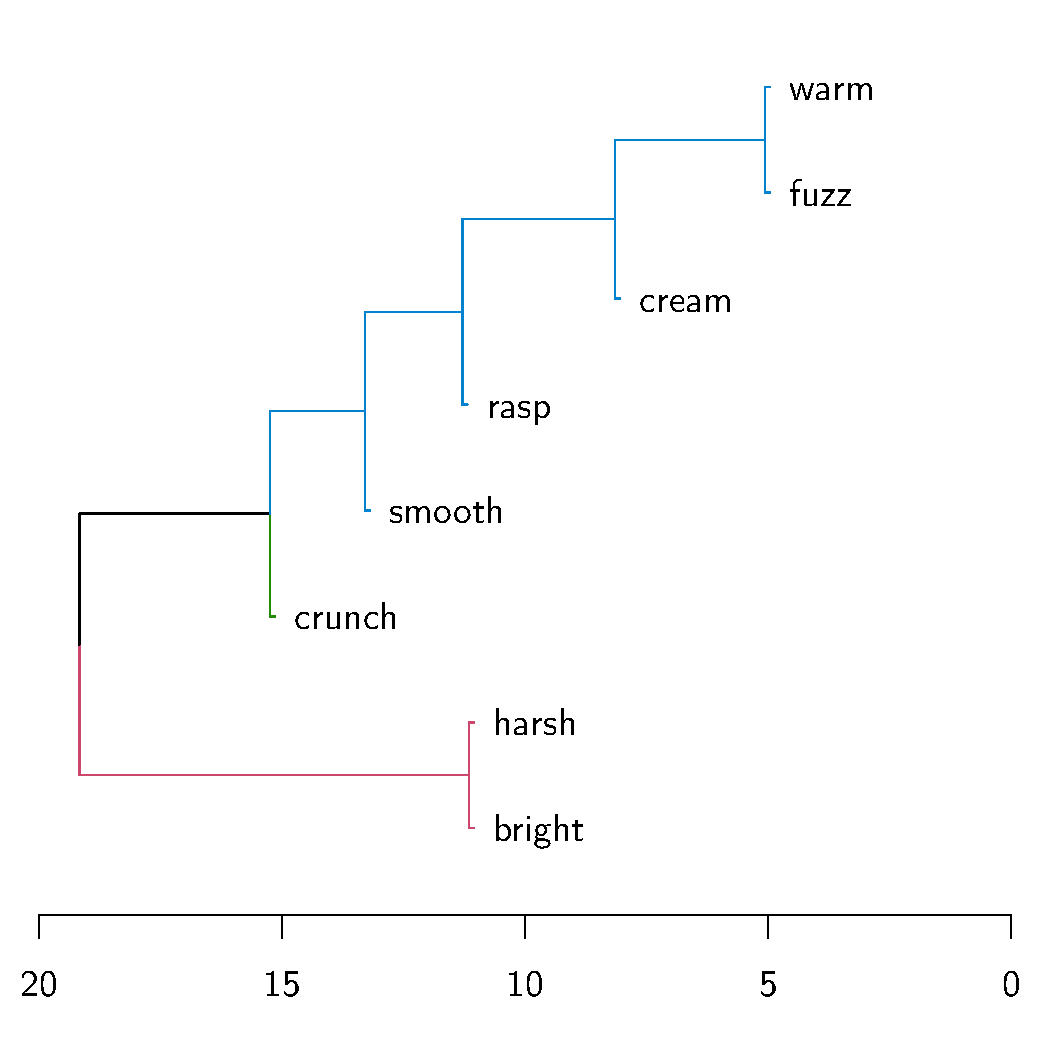
\includegraphics[width=0.45\textwidth]{chapter4/Images/DistortionProcessedClusters.pdf}
				\label{fig:DistortionProcessedClusters}
			}
			\qquad
			\subfloat[Feature Differences]
			{
				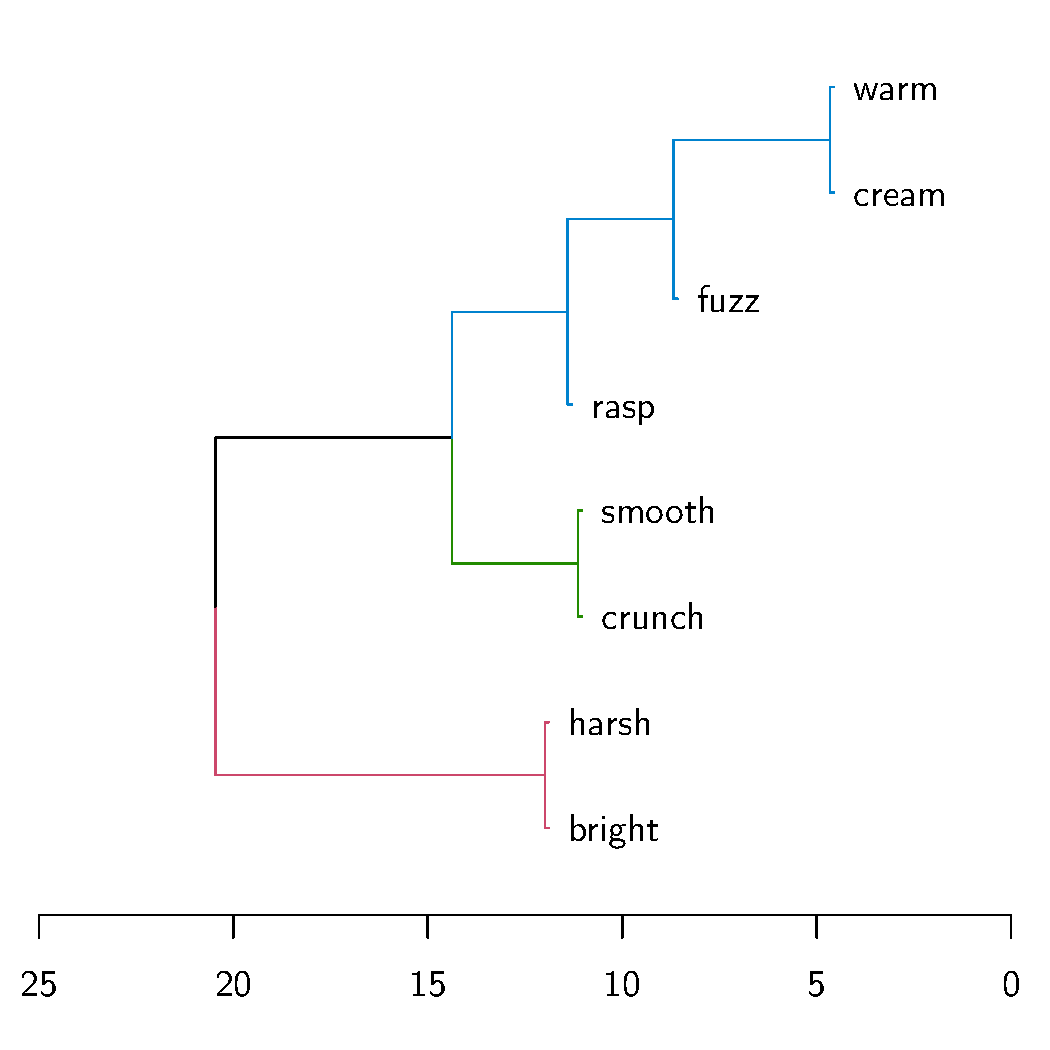
\includegraphics[width=0.45\textwidth]{chapter4/Images/DistortionDifferenceClusters.pdf}
				\label{fig:DistortionDifferenceClusters}
			}
			\caption{Clustering of descriptors from the distortion.}
			\label{fig:DistortionClusters}
		\end{figure}
		
		The clusters identified in the equaliser (Figure \ref{fig:EqualiserClusters}) show less agreement between
		the two different feature spaces. While the terms `warm' and `bright' were the most distant from each other
		in the distortion feature spaces, they are two of the closest terms in the equaliser's processed feature
		space (Figure \ref{fig:EqualiserProcessedClusters}). They are, however, separated well in the equaliser's
		feature difference space (Figure \ref{fig:EqualiserDifferenceClusters}) suggesting that these terms better
		describe a certain change in audio features rather than an absolute feature value.

		\note
		{
			Probably due to the large number of instances of bright and warm. There is a wide range of input
			signals meaning the processed features average out to be similar. The underlying transforms are
			distinct for each descriptor however.
		}
		
		Within the equaliser's feature differences space two main clusters are identified corresponding with the
		`warmth' and `brightness' clusters from the distortion feature spaces. The `warmth' cluster includes the
		terms `deep' and `full', while the `brightness' cluster includes the terms `tin', `thin', `clear' and
		`air'. An additional `boominess' cluster, containing `mud', `boom' and `box', is also present. These three
		terms cluster better in the processed feature space indicating that they are more likely to describe a
		particular set of feature values rather than the properties of a transform. There is a similarity between
		these clusters and the combinations of descriptors used to describe equaliser transforms (Table
		\ref{tab:EqualiserTermCombinations}) suggesting that some of these terms may be synonymous with each other.

		\begin{figure}[h!]
%		This figure is da baddest figure, ask your dyslexic down syndromed mother.
			\centering
			\subfloat[Processed Features]
			{
				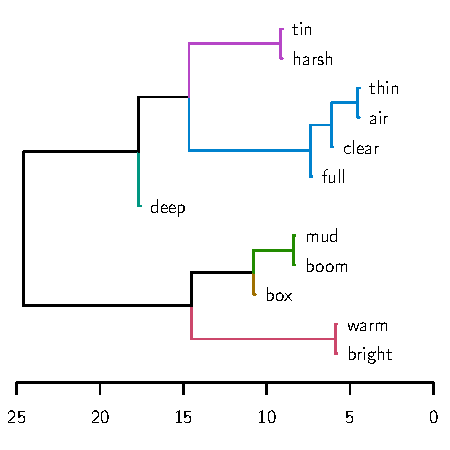
\includegraphics[width=0.45\textwidth]{chapter4/Images/EqualiserProcessedClusters.pdf}
				\label{fig:EqualiserProcessedClusters}
			}
			\qquad
			\subfloat[Feature Differences]
			{
				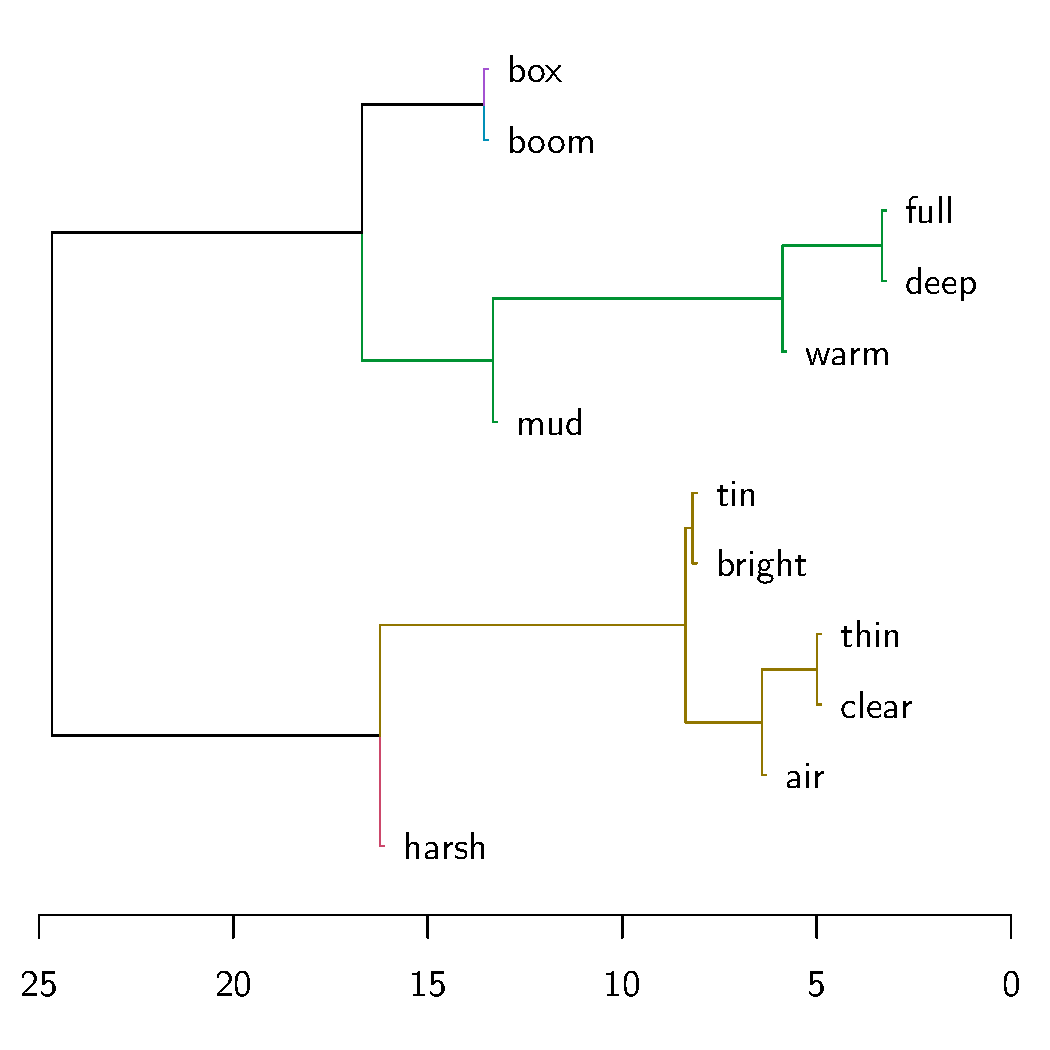
\includegraphics[width=0.45\textwidth]{chapter4/Images/EqualiserDifferenceClusters.pdf}
				\label{fig:EqualiserDifferenceClusters}
			}
			\caption{Clustering of descriptors from the equaliser.}
			\label{fig:EqualiserClusters}
		\end{figure}
		
		In order to investigate the similarity of descriptors across both plug-ins their respective feature spaces
		are combined and clustering is applied to produce the dendrograms shown in Figure
		\ref{fig:CombinedClusters}.  Each descriptors is prepended with the name of the plug-in it is associated
		with.

		\begin{figure}[h!]
			\centering
			\subfloat[Processed Features]
			{
				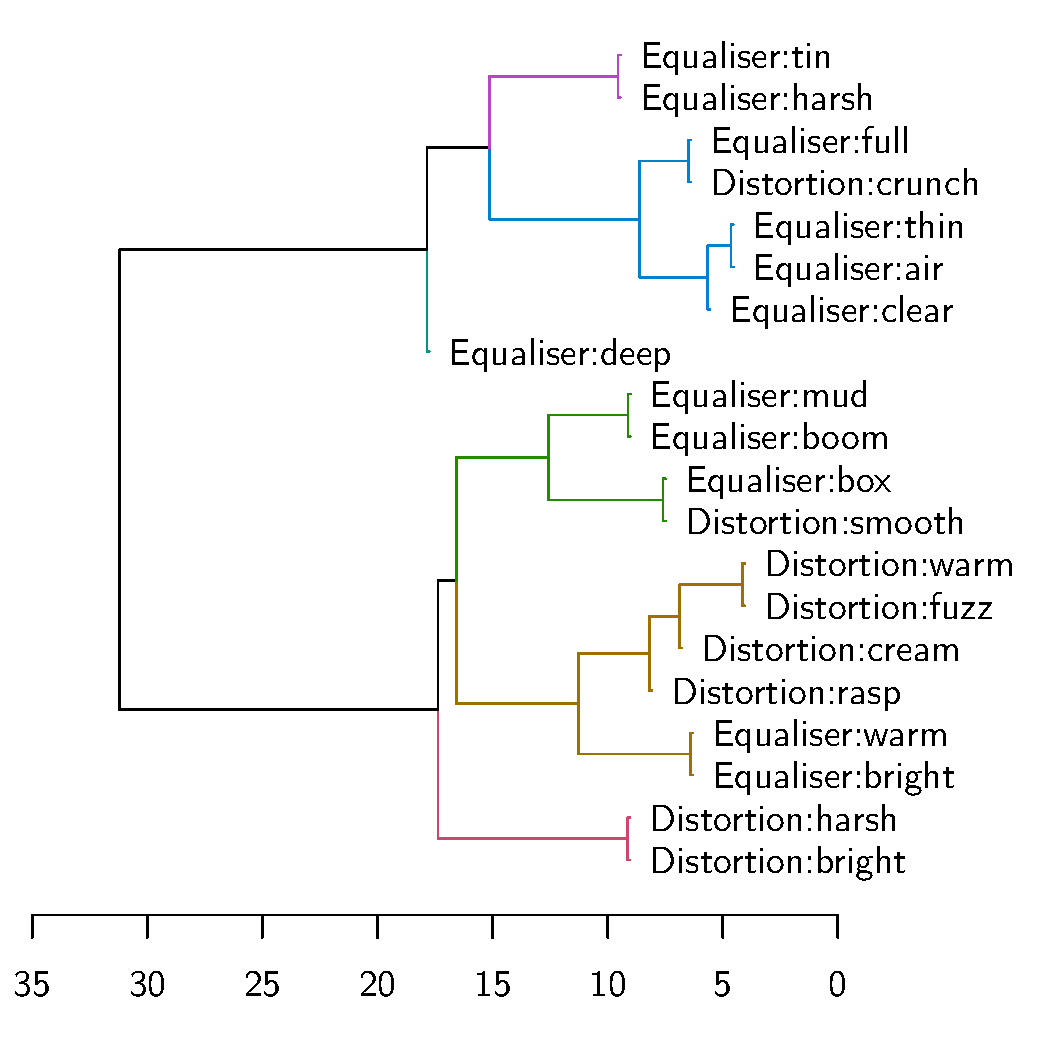
\includegraphics[width=0.45\textwidth]{chapter4/Images/CombinedProcessedClusters.pdf}
				\label{fig:CombinedProcessedClusters}
			}
			\qquad
			\subfloat[Feature Differences]
			{
				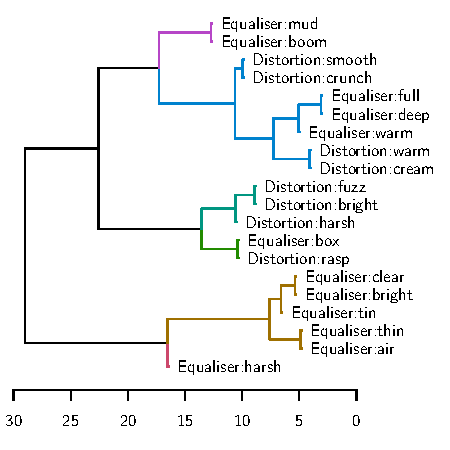
\includegraphics[width=0.45\textwidth]{chapter4/Images/CombinedDifferenceClusters.pdf}
				\label{fig:CombinedDifferenceClusters}
			}
			\caption{Clustering of descriptors from the both the distortion and equaliser.}
			\label{fig:CombinedClusters}
		\end{figure}

		Here the `warmth' clusters from each plug-in's features spaces are combined, indicating that each of these
		descriptors describe similar transforms regardless of the processing method used. In contrast the
		`brightness' groups remain separated into clusters comprised mostly of descriptors from a single plug-in,
		suggesting that the use of these terms may differ depending on the nature of the audio transform.  Further
		evidence of this is found in the similarity of the terms `bright' and `harsh'. When used to describe
		distortion transforms these terms always sit adjacent to one another in a cluster, whereas for equaliser
		transforms they are separated by a reasonable distance. These terms are more likely to be synonymous when
		describing audio processed by a static nonlinearity then they are for equalised audio. 

	\subsection{Agreement}
	\label{sec:TimbreEvaluation-Analysis-Agreement}
		In order to draw conclusions about the region a descriptor covers in a feature space, it is necessary to
		have a measure of agreement for a descriptor. This measure describes the level to which different users
		agree on the semantic meaning of descriptive terms. The closer together the transforms associated with a
		particular descriptor are grouped in the feature space, the higher that descriptor's agreement score.

		\citet{cartwright2013socialeq} measure how well participants agree on the semantic annotation of graphic
		equaliser parameter settings. For each participant a set of weightings is produced which describes the
		influence of each equaliser band on the perception of a particular timbral descriptor. The agreement score
		for a descriptor, $A(d)$, measures how similar these weightings are across different test participants
		using Equation \ref{eq:SocialEqAgreement}.

		\begin{equation}
			A(d) = \frac{\ln(N_{d})}{\sum_{k = 1}^{K} s_{d,k}^{2}}
			\label{eq:SocialEqAgreement}
		\end{equation}

		Where $N_{d}$ is the number of participants which have provided weightings for descriptor $d$,
		$s_{d,k}^{2}$ is the variance of weighting $k$ across those participants and $K$ is the number of
		weightings in each set (i.e. the number of equaliser bands). The logarithm of the number of
		participants is used to account for Zipf's law, which states that the frequency with which a word is used
		is inversely proportional to its usage ranking (an integer describing the words popularity; 1 denoting the
		most commonly used word, 2 the second most common etc.) \citep{manning1999foundations}.

		This can be applied to data from the SAFE plug-ins by using audio feature values in place of parameter
		weightings. In Equation \ref{eq:SocialEqAgreement}, $N_{d}$ is then the number of transforms labelled with
		descriptor $d$, $s_{d,k}^{2}$ is the variance of feature $k$ across those transforms and $K$ is the
		number of features. As when clustering, the feature space should be standardised prior to calculating
		agreement to remove the biasing effects caused by the ranges of each feature.

		This agreement measure has several properties which do not necessarily reflect what is being measured:

		\begin{itemize}
			\item A larger number of transforms, $N_{d}$, produces higher agreement.
			\item It is assumed that high variance in any feature implies a disagreement. 
			\item It is assumed that all audio features are independent. 
			\item It is assumed that low variance in any feature implies an agreement. 
		\end{itemize}

		In this section an agreement measure which accounts for these points is developed.

		\subsubsection*{Number of Transforms}
			In Equation \ref{eq:SocialEqAgreement} the logarithm of the number of transforms, $N_{d}$, is used
			to scale the agreement score. This measures a different concept of agreement to what we desire for
			this work. Rather than measuring the size of the region a descriptor occupies in the feature space,
			it measure how many individual transforms make up that region. A sufficiently large number of
			transforms will produce a large agreement score regardless of how spread apart they are. To measure
			the size of the region a descriptor occupies, the scaling factor should be removed giving Equation
			\ref{eq:ReciprocalOfSumAgreement}.

			\begin{equation}
				A(d) = \frac{1}{\sum_{k = 1}^{K} s_{d,k}^{2}}
				\label{eq:ReciprocalOfSumAgreement}
			\end{equation}

			To take account of the number of transforms labelled with a particular descriptor, Bessel's
			correction can be used in the calculation of variance as shown in Equation
			\ref{eq:UnbiasedVariance}. This uses the data available from a sample and uses it to approximate
			the variation present in the population.

			\begin{equation}
				s_{d,k}^{2} = \frac{1}{N_{d} - 1} \sum_{n = 1}^{N_{d}} (x_{d,k,n} - \bar{x}_{d,k})^{2}
				\label{eq:UnbiasedVariance}
			\end{equation}

			Where $x_{d,k,n}$ is the value of feature $k$ for the $n$\super{th} transform labelled with
			descriptor $d$ and $\bar{x}_{d,k}$ is the mean value of feature $k$ across all transforms labelled
			with descriptor $d$.

			Using this measure of variance in the agreement score provides an approximation of how closely
			clustered transforms, labeled with a certain descriptor, would be in a feature space which
			represents the whole population. In all further agreement score calculations it is assumed that the
			variances, or covariances, are measured using Bessel's correction.

		\subsubsection*{High Variance}
			A term exhibiting high variance in a particular audio feature could imply one of two things. Either
			that users do not agree on the position of the term in the feature space, or that that feature has
			no effect on the perception of the term. In the first case the agreement score should be decreased,
			but in the second the agreement score should not be affected. Because of this ambiguity, it is
			preferable that a high variance has negligible effect on the agreement score. In this way, if a
			high variance does imply disagreement it does not unduly increase the agreement score and if at
			does not imply disagreement it does to unduly decrease the agreement score.
			
			This can be implemented by changing Equation \ref{eq:ReciprocalOfSumAgreement} to be a sum of
			reciprocals rather than the reciprocal of a sum, as shown in Equation
			\ref{eq:SumOfReciprocalAgreement}.

			\begin{equation}
				A(d) = \sum_{k = 1}^{K} \frac{1}{s_{d,k}^{2}}
				\label{eq:SumOfReciprocalAgreement}
			\end{equation}

		\subsubsection*{Dependent Features}
			It may be the case that users agree that a particular term describes a relationship between several
			audio features (e.g. a spectral centroid lying at the 4\super{th} harmonic). Equations
			\ref{eq:SocialEqAgreement}, \ref{eq:ReciprocalOfSumAgreement} and \ref{eq:SumOfReciprocalAgreement}
			all ignore any dependence between audio features.

			Relationships between features can be taken into account by calculating the covariance matrix for
			the transforms associated with a term. The variances in each feature can then be substituted with
			the eigenvalues of this matrix, as shown in Equation \ref{eq:EigenvalueAgreement}.

			\begin{equation}
				A(d) = \sum_{k = 1}^{K} \frac{1}{\lambda_{d,k}}
				\label{eq:EigenvalueAgreement}
			\end{equation}
			
			Where $\lambda_{d, k}$ is the $k$\super{th} eigenvalue of the covariance matrix for all transforms
			labelled with descriptor $d$.

			When using Equation \ref{eq:EigenvalueAgreement}, the number of eigenvalues used, $K$, needs to be
			carefully selected. If $N_{d}$ is less than or equal to the total number of audio features, the
			covariance matrix will be singular, meaning it will have one or more eigenvalues equal to zero. At
			most, only the $N_{d} - 1$ largest eigenvalues should be used.
			
			Any other eigenvalues equal to zero would imply a perfect linear relationship between a combination
			of audio features. If the features concerned are mathematically defined to be directly proportional
			then these zero eigenvalues should have no effect on the agreement score. If, however, a perfect
			linear relationship is discovered in the data, the agreement score should be increased
			accordingly. This raises an issue with Equation \ref{eq:EigenvalueAgreement} in that a devision by
			zero will occur if a perfectly linear relationship is discovered. This can be remedied by
			calculating the agreement using Equation \ref{eq:BoundedEigenvalueAgreement}. Calculating the
			agreement in this manner also has the advantage of bounding the agreement score between zero (no
			agreement) and $K$ (perfect agreement in all dimensions).

			\begin{equation}
				A(d) = \sum_{k = 1}^{K} \frac{1}{1 + \lambda_{d,k}}
				\label{eq:BoundedEigenvalueAgreement}
			\end{equation}

		\subsubsection*{Low Variance}
			Low variance in a particular audio feature does not necessarily imply an agreement between users.
			It may indicate a similarity between all of the audio segments processed, regardless of semantic
			labelling. To account for this, features which have low variance across the entire dataset can be
			disregarded. This can be achieved by calculating the agreement in a reduced dimensionality feature
			space.

			Using PCA, the dimensions with the largest variance in the feature space can be discovered. If the
			transforms labelled with a particular term exhibit a small variance in one of these dimensions it
			is likely that that term is well agreed upon. Agreement can be calculated in the PCA timbre space
			using Equation \ref{eq:BoundedEigenvalueAgreement}, with $\lambda_{d,k}$ being the $k$\super{th}
			eigenvalue of the covariance matrix of the principal components (PCs) for every transform labelled
			with descriptor $d$. As when calculating the agreement in the feature space, the coordinates of the
			transforms in each PC should be standardised to remove bias introduced by the proportions of total
			variance each PC describes.

			The number of PCs to used in the calculation of agreement is an important consideration. PCs which
			describe a low proportion of total variance should be discarded as is can not be known whether this
			low variance is due to user agreement. It is therefore recommended that a threshold is set, and
			only PCs which describe a proportion of variance above this threshold are used. Discarding the low
			variance PCs in this manner also removes any which have zero variance due to audio features
			which are defined to be directly proportional to one another, removing their effect on the
			agreement score.

			Further to this, the number of eigenvalues used, $K$, needs to be decided. Where $N_{d}$ is greater
			than the number of PCs used, all the eigenvalues should be used ($K$ equal to the number of PCs).
			For cases where $N_{d}$ is less than or equal to the number of PCs used, only $N_{d} - 1$
			eigenvalues should be used ($K = N_{d} - 1$). This dynamic value for $K$ has the benefit of
			reducing the agreement scores for terms which describe very few transforms. It also ensures that
			terms which describe only one transform will always receive an agreement score of zero, as $K$ will
			be equal to zero.

		\subsubsection*{Validation with Synthesised Data}
			To demonstrate the differences between Equations \ref{eq:SocialEqAgreement},
			\ref{eq:ReciprocalOfSumAgreement}, \ref{eq:SumOfReciprocalAgreement}, \ref{eq:EigenvalueAgreement}
			and \ref{eq:BoundedEigenvalueAgreement} artificial data can be synthesised which exhibits some of
			the issues discussed with Equation \ref{eq:SocialEqAgreement}.
			
			Figure \ref{fig:SynthesisedData} shows a synthesised, three dimensional, dataset containing four
			clusters of points. For ease of discussion it is assumed that this data represents the feature
			space after PCA has been applied. Each cluster has different properties which need to be taken into
			account when calculating the agreement score. Cluster 1 represents a set of points whose position
			in the PCA space is not agreed upon, exhibiting a high variance in every PC. Cluster 2 represents a
			set of points whose position is very well agreed upon, having low variance in every PC. Cluster 3
			represents a set of points whose position is only defined in one PC, having high variance in the
			other two. Cluster 4 represent a set of points which are defined by a relationship between two PCs,
			exhibiting high variance in all PCs but a strong correlation ($p = 0.9$) between PCs 1 and 2. The
			clusters were generated using the techniques discussed by \citet{ripley1987stochastic}, using the
			means, $\mu$, and covariance matrices, $\Sigma$, shown in Datum \ref{dat:ClusterStats}.

			\begin{datum}[h!]
				\centering
				\subfloat[Cluster 1]
				{
					\parbox{5cm}
					{
						\centering
						$\mu = \begin{bmatrix}
							     2 & 3 & 4
						       \end{bmatrix}$

						\vspace{1em}

						$\Sigma = \begin{bmatrix}
								5 & 0 & 0 \\
								0 & 5 & 0 \\
								0 & 0 & 5
							  \end{bmatrix}$
					}
					\label{dat:Cluster1Stats}
				}
				\qquad
				\subfloat[Cluster 2]
				{
					\parbox{5cm}
					{
						\centering
						$\mu = \begin{bmatrix}
							     4 & -2 & 1
						       \end{bmatrix}$

						\vspace{1em}

						$\Sigma = \begin{bmatrix}
								0.2 & 0 & 0 \\
								0 & 0.2 & 0 \\
								0 & 0 & 0.2
							  \end{bmatrix}$
					}
					\label{dat:Cluster2Stats}
				}

				\vspace{1.5em}

				\subfloat[Cluster 3]
				{
					\parbox{5cm}
					{
						\centering
						$\mu = \begin{bmatrix}
							     -2 & 0 & 2
						       \end{bmatrix}$

						\vspace{1em}

						$\Sigma = \begin{bmatrix}
								0.1 & 0 & 0 \\
								0 & 6 & 0 \\
								0 & 0 & 5
							  \end{bmatrix}$
					}
					\label{dat:Cluster3Stats}
				}
				\qquad
				\subfloat[Cluster 4]
				{
					\parbox{5cm}
					{
						\centering
						$\mu = \begin{bmatrix}
							     5 & -3 & 4
						       \end{bmatrix}$

						\vspace{1em}

						$\Sigma = \begin{bmatrix}
								5 & 0.9\sqrt{10} & 0 \\
								0.9\sqrt{10} & 2 & 0 \\
								0 & 0 & 4
							  \end{bmatrix}$
					}
					\label{dat:Cluster4Stats}
				}
				\caption{The means and covariance matrices for the clusters shown in Figure
					 \ref{fig:SynthesisedData}.}
				\label{dat:ClusterStats}
			\end{datum}

			\begin{figure}[h!]
				\centering
				\subfloat
				{
					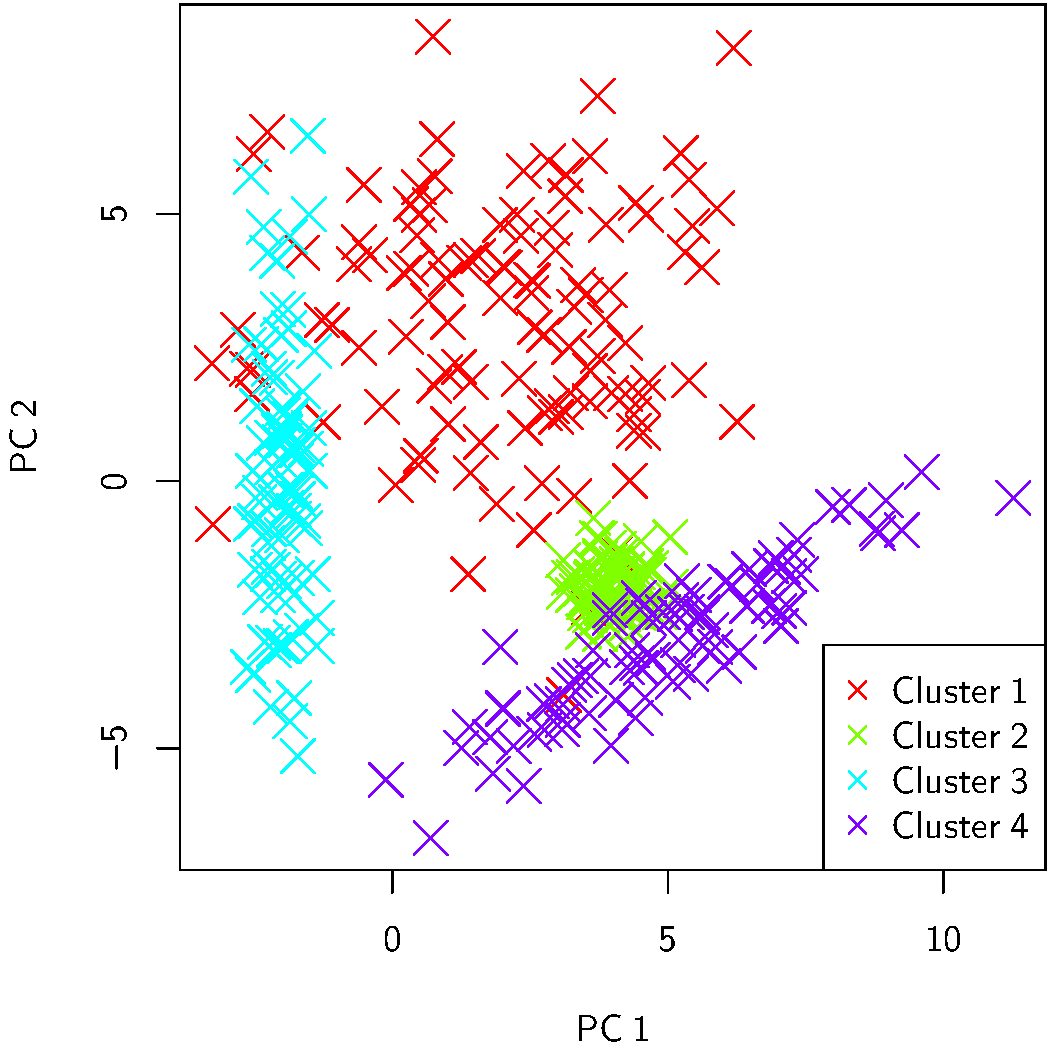
\includegraphics[width=0.45\textwidth]{chapter4/Images/ArtificialData1-2.pdf}
					\label{fig:EqualiserDifferencePCA}
				}
				\qquad
				\subfloat
				{
					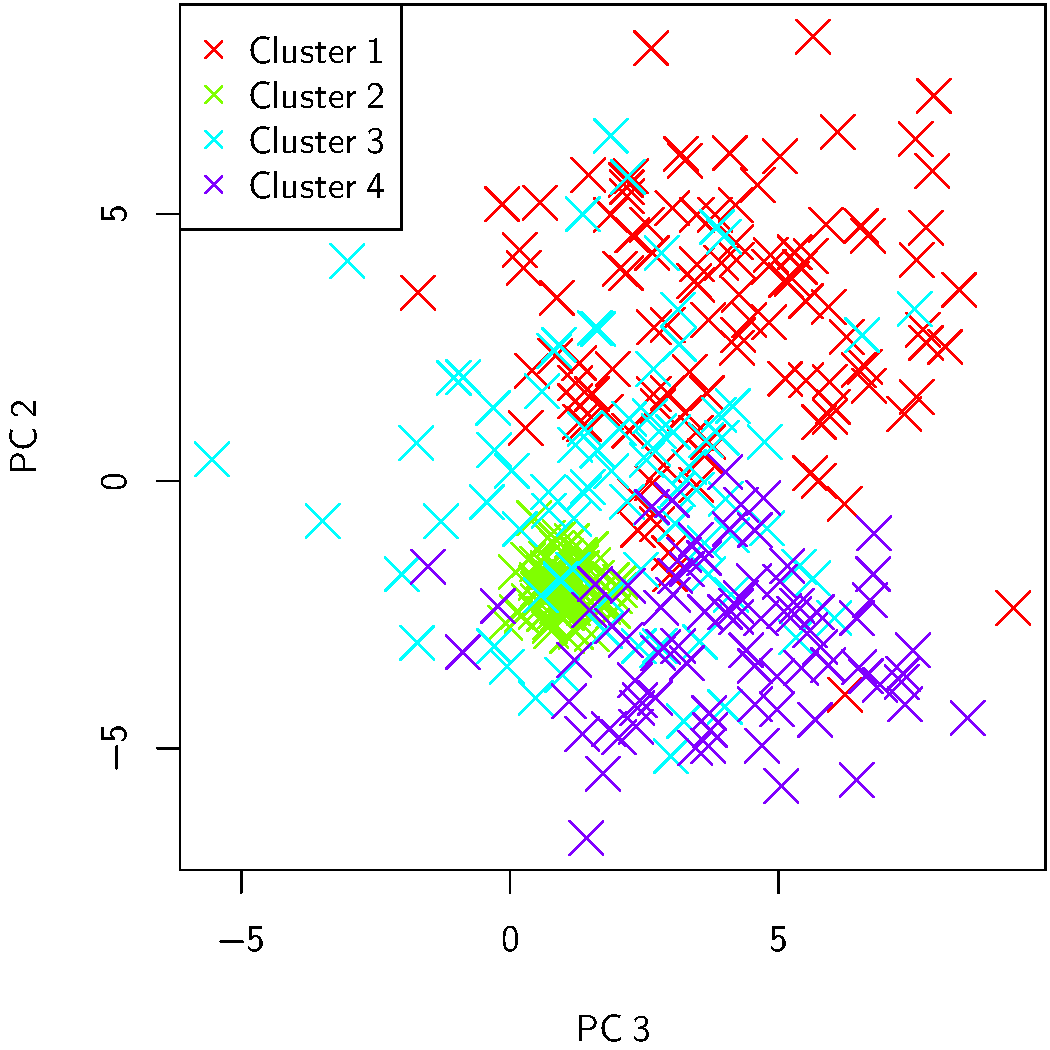
\includegraphics[width=0.45\textwidth]{chapter4/Images/ArtificialData3-2.pdf}
					\label{fig:EqualiserDifferenceCentroidsPCA}
				}
				\caption{Synthesised Data.}
				\label{fig:SynthesisedData}
			\end{figure}

			Visualising the data in Figure \ref{fig:SynthesisedData} provides intuition as to how an agreement
			score should rate each cluster. Cluster 1 should receive the lowest score as there is no
			discernible pattern to the data points. Cluster 2 should receive the highest score as it is very
			tightly clustered in all PCs. Both clusters 3 and 4 show some some patterns in the distribution.
			Cluster 3 has a well defined position in PC 1 while cluster 4 shows a strong relationship between
			PCs 1 and 2. The agreement scores for these clusters should reflect these patterns. Table
			\ref{tab:SynthesisedDataAgreement} shows agreement scores for the data shown in Figure
			\ref{fig:SynthesisedData}, calculated using Equations \ref{eq:SocialEqAgreement},
			\ref{eq:ReciprocalOfSumAgreement}, \ref{eq:SumOfReciprocalAgreement}, \ref{eq:EigenvalueAgreement}
			and \ref{eq:BoundedEigenvalueAgreement}.

			\begin{table}[h!]
				\centering
				\begin{tabular}{|c|c|c|c|c|c|}
					\cline{2-6}
					\multicolumn{1}{c|}{} & \multicolumn{5}{c|}{\bf{Agreement Score}} \tabularnewline
					\hline
					\bf{Cluster} & \bf{Equation \ref{eq:SocialEqAgreement}} & 
					\bf{Equation \ref{eq:ReciprocalOfSumAgreement}} &
					\bf{Equation \ref{eq:SumOfReciprocalAgreement}} & 
					\bf{Equation \ref{eq:EigenvalueAgreement}} &
					\bf{Equation \ref{eq:BoundedEigenvalueAgreement}} \tabularnewline
					\hline
					\hline
					\bf{1} & 2.3 & 0.5 & 4.7 & 4.7 & 1.8 \tabularnewline
					\hline
					\bf{2} & 55.1 & 12.2 & 117.9 & 117.9 & 2.9 \tabularnewline
					\hline
					\bf{3} & 2.7 & 0.6 & 95.7 & 95.7 & 2.1 \tabularnewline
					\hline
					\bf{4} & 2.9 & 0.7 & 7.7 & 34.8 & 2.1 \tabularnewline
					\hline
				\end{tabular}
				\caption{Agreement scores for the synthesised data.}
				\label{tab:SynthesisedDataAgreement}
			\end{table}

			The issues with Equations \ref{eq:SocialEqAgreement} and \ref{eq:ReciprocalOfSumAgreement} are
			immediately obvious. They ignore readily noticeable patterns in the data, giving clusters 1, 3 and
			4 similar agreement scores. By removing the assumption that high variance implies disagreement,
			Equation \ref{eq:SumOfReciprocalAgreement} takes account of the pattern in cluster 3. Equation
			\ref{eq:EigenvalueAgreement} removes the assumption that all PCs are independent enabling it to
			reflect the pattern shown in cluster 4. The final column of Table
			\ref{tab:SynthesisedDataAgreement} shows the bounding effect given by Equation
			\ref{eq:BoundedEigenvalueAgreement}.

	\subsection{Timbre Spaces}
	\label{sec:TimbreEvaluation-Analysis-TimbreSpaces}
		Clustering provides insight into the similarity of descriptive terms but does not show what properties of
		the signals / transforms contribute to the differences between descriptor clusters. Reducing the
		dimensionality of the audio feature space allows for the most salient features to be identified. To
		preserve as much of the audio feature data as possible, a different feature space, to that used for
		clustering, is constructed. Rather than each descriptor representing one point in the feature space, each
		individual transform represents its own point. In this manner dimensions which have little effect on a
		certain timbral descriptor are easily determined. The points labeled with a particular term will be more
		spread out across the dimensions which do not affect them. 
		
		Prior to analysis, the feature spaces are standardised to remove any bias caused by features with a large
		range. PCA is then applied in order to create the low dimensionality timbre spaces discussed in this
		section. Two different types of plot are used to identify patterns within these timbre spaces. The first is
		a scatter plot in which the position of each individual transform is shown. These plots shoe the regions of
		the timbre space that certain terms describe. The second is a biplot showing the mean position of
		transforms labelled with each descriptor along with vectors showing the influence of selected audio
		features. In these graphs the size of the text indicates the agreement score associated with that
		descriptor.

		\subsubsection*{Distortion Processed Features}
			\begin{itemize}
				\item {\bf{PC 1:}} $\textrm{KI}$~($p~=~-0.992$), $\textrm{KI}_{\textrm{p}}$~($p~=~-0.985$),
					$\textrm{KI}_{\textrm{h}}$~($p~=~-0.968$), $\kappa_{\textrm{p}}$~($p~=~-0.964$),
					$\kappa_{\textrm{h}}$~($p~=~-0.959$), $\gamma_{\textrm{p}}$~($p~=~-0.957$),
					$\gamma_{\textrm{h}}$~($p~=~-0.946$), $\gamma_{\textrm{s}}$~($p~=~-0.923$),
					$\sigma$~($p~=~-0.919$), $\textrm{RMS}$~($p~=~-0.919$),
					$\sigma^{2}$~($p~=~-0.851$), $\kappa_{\textrm{s}}$~($p~=~-0.790$).
				\item {\bf{PC 2:}} $\textrm{SRO}$~($p~=~ 0.938$), $\sigma_{\textrm{h}}$~($p~=~ 0.933$),
					$\sigma_{\textrm{p}}$~($p~=~ 0.932$), $\mu_{\textrm{p}}$~($p~=~ 0.904$),
					$\mu_{\textrm{h}}$~($p~=~ 0.903$), $\textrm{ZCR}$~($p~=~ 0.875$),
					$\mu_{\textrm{s}}$~($p~=~ 0.856$), $\textrm{MFCC}_{1}$~($p~=~-0.851$),
					$\textrm{SSl}$~($p~=~ 0.827$), $\sigma_{\textrm{p}}^{2}$~($p~=~ 0.788$),
					$\sigma_{\textrm{h}}^{2}$~($p~=~ 0.786$).
				\item {\bf{PC 3:}} $\textrm{MFCC}_{2}$~($p~=~ 0.787$), $\textrm{MFCC}_{4}$~($p~=~ 0.774$),
					$T_{\textrm{p}3}$~($p~=~-0.722$), $T_{3}$~($p~=~-0.704$).
			\end{itemize}

			\begin{figure}[h!]
				\centering
				\subfloat[Individual Transforms]
				{
					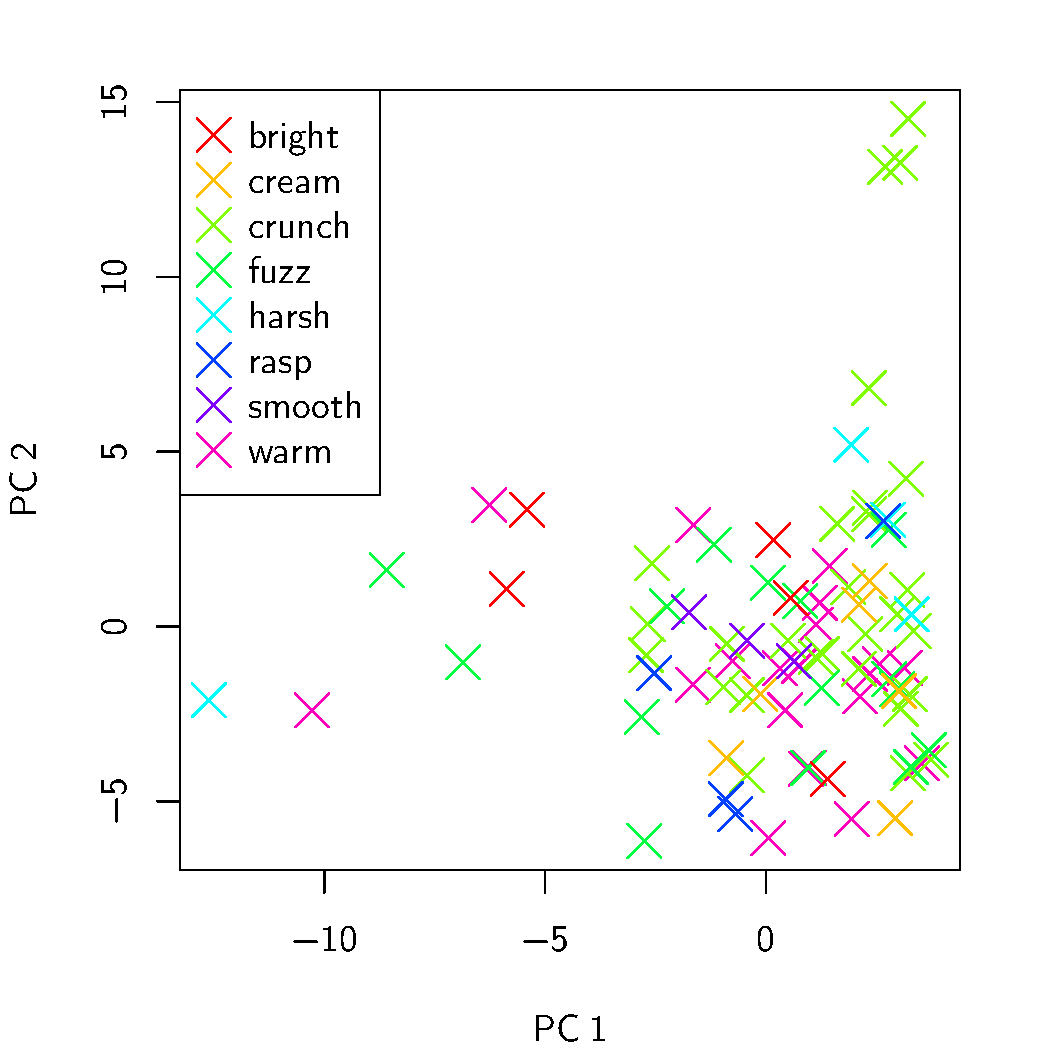
\includegraphics[width=0.45\textwidth]{chapter4/Images/DistortionProcessedPCA.pdf}
					\label{fig:DistortionProcessedPCA}
				}
				\qquad
				\subfloat[Descriptor Centroids]
				{
					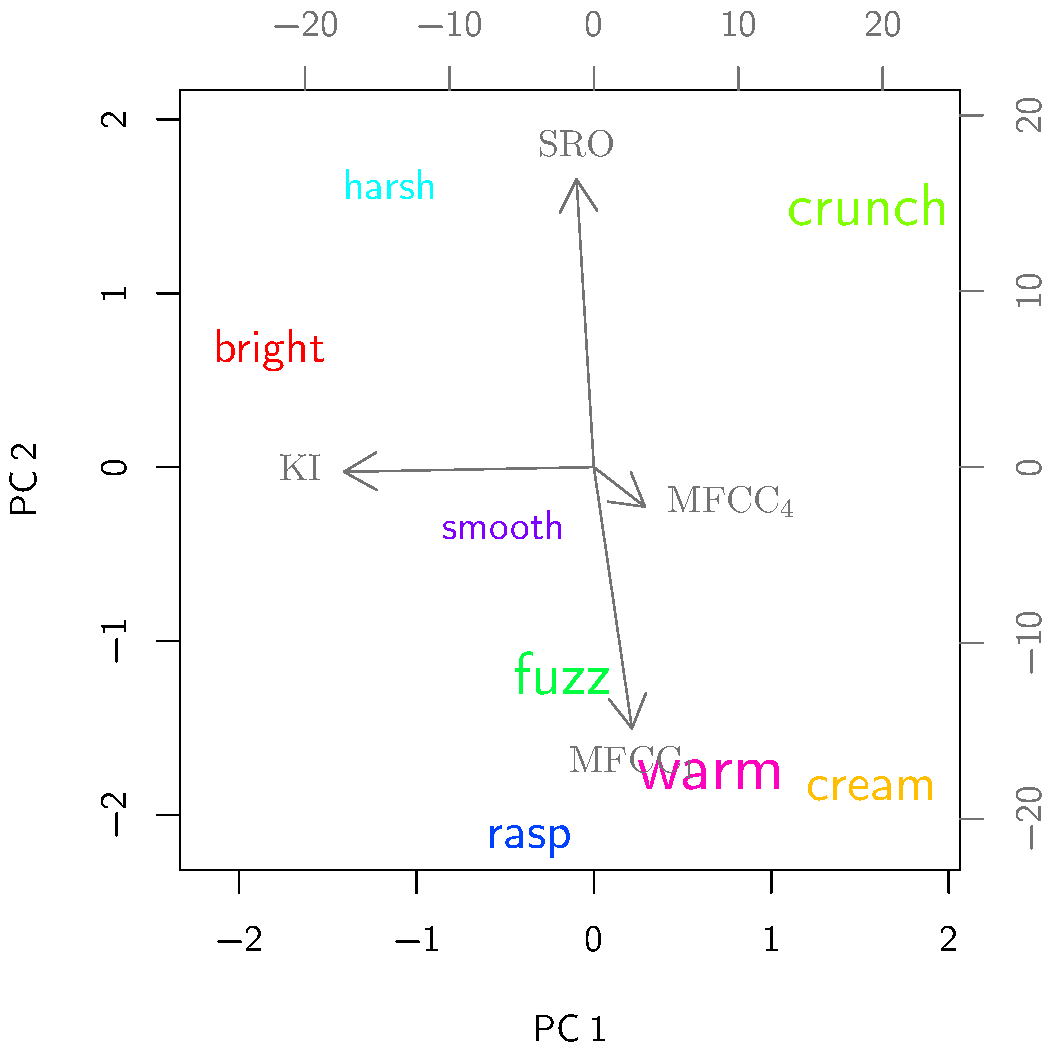
\includegraphics[width=0.45\textwidth]
							{chapter4/Images/DistortionProcessedCentroidsPCA.pdf}
					\label{fig:DistortionProcessedCentroidsPCA}
				}
				\caption{Timbre space for the processed features from the distortion.}
				\label{fig:DistortionProcessedPCAs}
			\end{figure}

		\subsubsection*{Distortion Feature Differences}
			\begin{itemize}
				\item {\bf{PC 1:}} $\textrm{KI}$~($p~=~0.992$), $\textrm{KI}_{\textrm{p}}$~($p~=~0.989$),
					$\textrm{KI}_{\textrm{h}}$~($p~=~0.971$), $\gamma_{\textrm{p}}$~($p~=~0.956$),
					$\kappa_{\textrm{p}}$~($p~=~0.956$), $\gamma_{\textrm{h}}$~($p~=~0.943$),
					$\kappa_{\textrm{h}}$~($p~=~0.941$), $\sigma$~($p~=~0.939$),
					$\textrm{RMS}$~($p~=~0.939$), $\gamma_{\textrm{s}}$~($p~=~0.918$),
					$\sigma^{2}$~($p~=~0.877$), $\kappa_{\textrm{s}}$~($p~=~0.744$).
				\item {\bf{PC 2:}} $\textrm{SRO}$~($p~=~-0.913$), $\mu_{\textrm{s}}$~($p~=~-0.901$),
					$\sigma_{\textrm{h}}$~($p~=~-0.869$), $\mu_{\textrm{h}}$~($p~=~-0.832$),
					$\sigma_{\textrm{p}}$~($p~=~-0.831$), $\mu_{\textrm{p}}$~($p~=~-0.830$),
					$\textrm{SSl}$~($p~=~-0.793$), $\sigma_{\textrm{s}}^{2}$~($p~=~-0.764$),
					$\sigma_{\textrm{s}}$~($p~=~-0.761$), $\sigma_{\textrm{p}}^{2}$~($p~=~-0.725$),
					$\sigma_{\textrm{h}}^{2}$~($p~=~-0.719$), $\textrm{ZCR}$~($p~=~-0.715$).
				\item {\bf{PC 3:}} $T_{1}$~($p~=~-0.797$), $T_{\textrm{p}1}$~($p~=~-0.783$).
			\end{itemize}

			\begin{figure}[h!]
				\centering
				\subfloat[Individual Transforms]
				{
					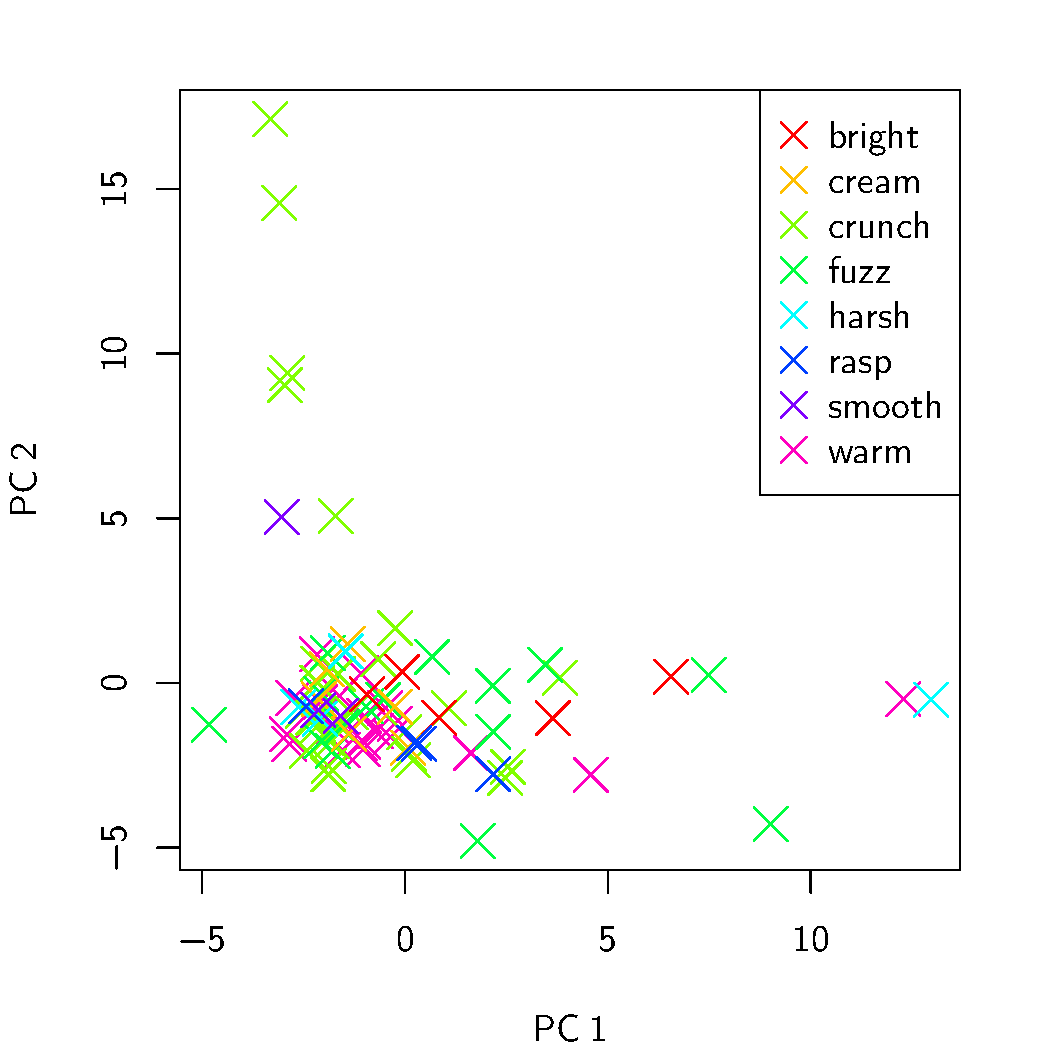
\includegraphics[width=0.45\textwidth]{chapter4/Images/DistortionDifferencePCA.pdf}
					\label{fig:DistortionDifferencePCA}
				}
				\qquad
				\subfloat[Descriptor Centroids]
				{
					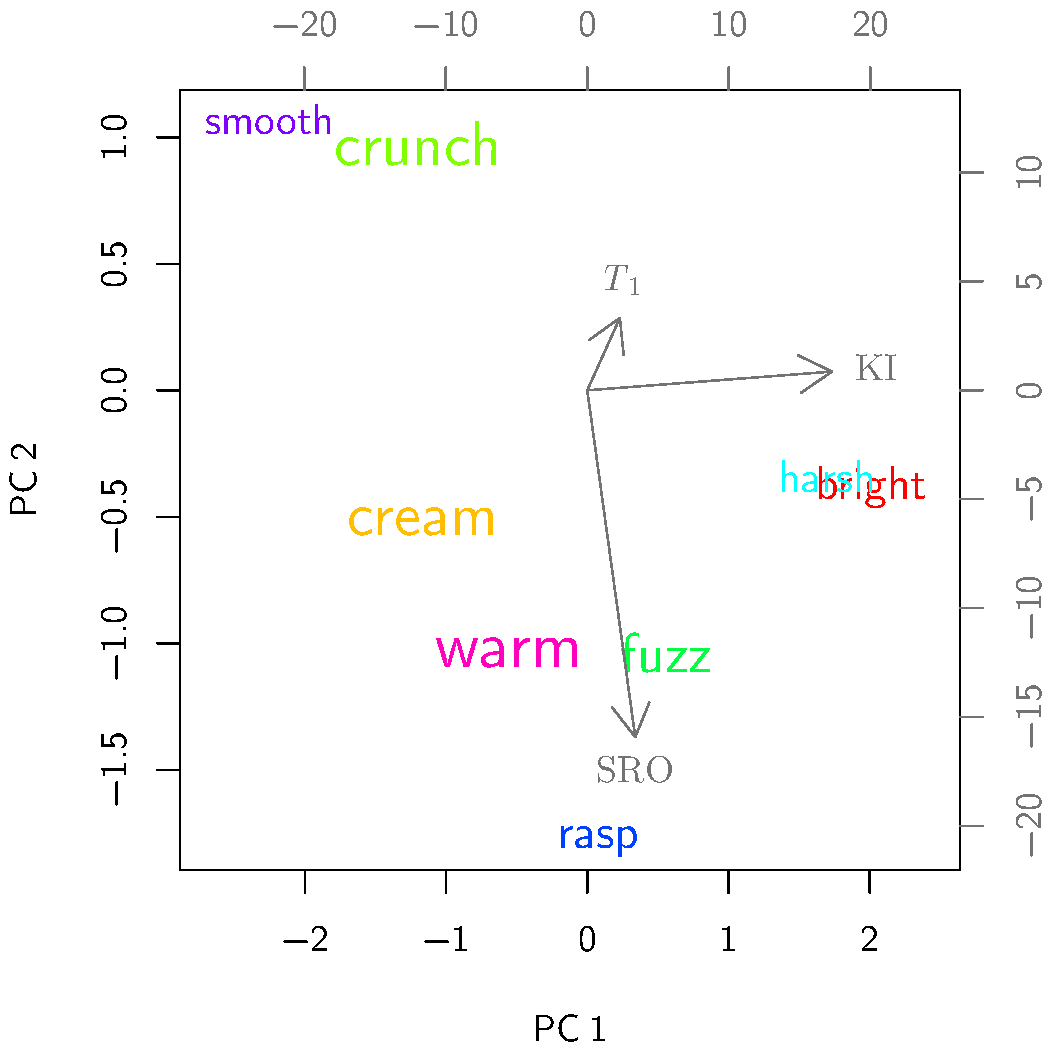
\includegraphics[width=0.45\textwidth]
							{chapter4/Images/DistortionDifferenceCentroidsPCA.pdf}
					\label{fig:DistortionDifferenceCentroidsPCA}
				}
				\caption{Timbre space for the feature differences from the distortion.}
				\label{fig:DistortionDifferencePCAs}
			\end{figure}

		\subsubsection*{Equaliser Processed Features}
			\begin{itemize}
				\item {\bf{PC 1:}} $\textrm{KI}$~($p~=~0.991$), $\textrm{KI}_{\textrm{p}}$~($p~=~0.981$),
					$\kappa_{\textrm{h}}$~($p~=~0.966$), $\kappa_{\textrm{p}}$~($p~=~0.962$),
					$\textrm{KI}_{\textrm{h}}$~($p~=~0.958$), $\gamma_{\textrm{s}}$~($p~=~0.945$),
					$\gamma_{\textrm{p}}$~($p~=~0.895$), $\gamma_{\textrm{h}}$~($p~=~0.886$),
					$\kappa_{\textrm{s}}$~($p~=~0.884$), $\sigma$~($p~=~0.840$),
					$\textrm{RMS}$~($p~=~0.840$), $\sigma^{2}$~($p~=~0.813$).
				\item {\bf{PC 2:}} $\sigma_{\textrm{h}}$~($p~=~ 0.922$), $\sigma_{\textrm{p}}$~($p~=~
					0.918$), $\textrm{SRO}$~($p~=~ 0.895$), $\mu_{\textrm{h}}$~($p~=~ 0.881$),
					$\mu_{\textrm{p}}$~($p~=~ 0.881$), $\mu_{\textrm{s}}$~($p~=~ 0.806$),
					$\textrm{SSl}$~($p~=~ 0.805$), $\textrm{MFCC}_{1}$~($p~=~-0.802$),
					$\textrm{ZCR}$~($p~=~ 0.798$), $\sigma_{\textrm{p}}^{2}$~($p~=~ 0.761$),
					$\sigma_{\textrm{h}}^{2}$~($p~=~ 0.761$), $T_{\textrm{p}2}$~($p~=~-0.749$),
					$T_{2}$~($p~=~-0.745$), $\textrm{SC}$~($p~=~-0.720$).
				\item {\bf{PC 3:}} $\textrm{MFCC}_{4}$~($p~=~-0.718$), $\textrm{MFCC}_{2}$~($p~=~-0.715$),
					$\sigma_{\textrm{s}}$~($p~=~-0.714$).
				\item {\bf{PC 4:}} $\textrm{MFCC}_{8}$~($p~=~0.926$), $\textrm{MFCC}_{10}$~($p~=~0.839$),
					$\textrm{MFCC}_{9}$~($p~=~0.836$), $\textrm{MFCC}_{12}$~($p~=~0.760$),
					$\textrm{MFCC}_{7}$~($p~=~0.725$), $\textrm{MFCC}_{11}$~($p~=~0.721$).
				\item {\bf{PC 5:}} $\textrm{MFCC}_{5}$~($p~=~0.743$), $\textrm{MFCC}_{3}$~($p~=~0.705$).
			\end{itemize}

			\begin{figure}[h!]
				\centering
				\subfloat[Individual Transforms]
				{
					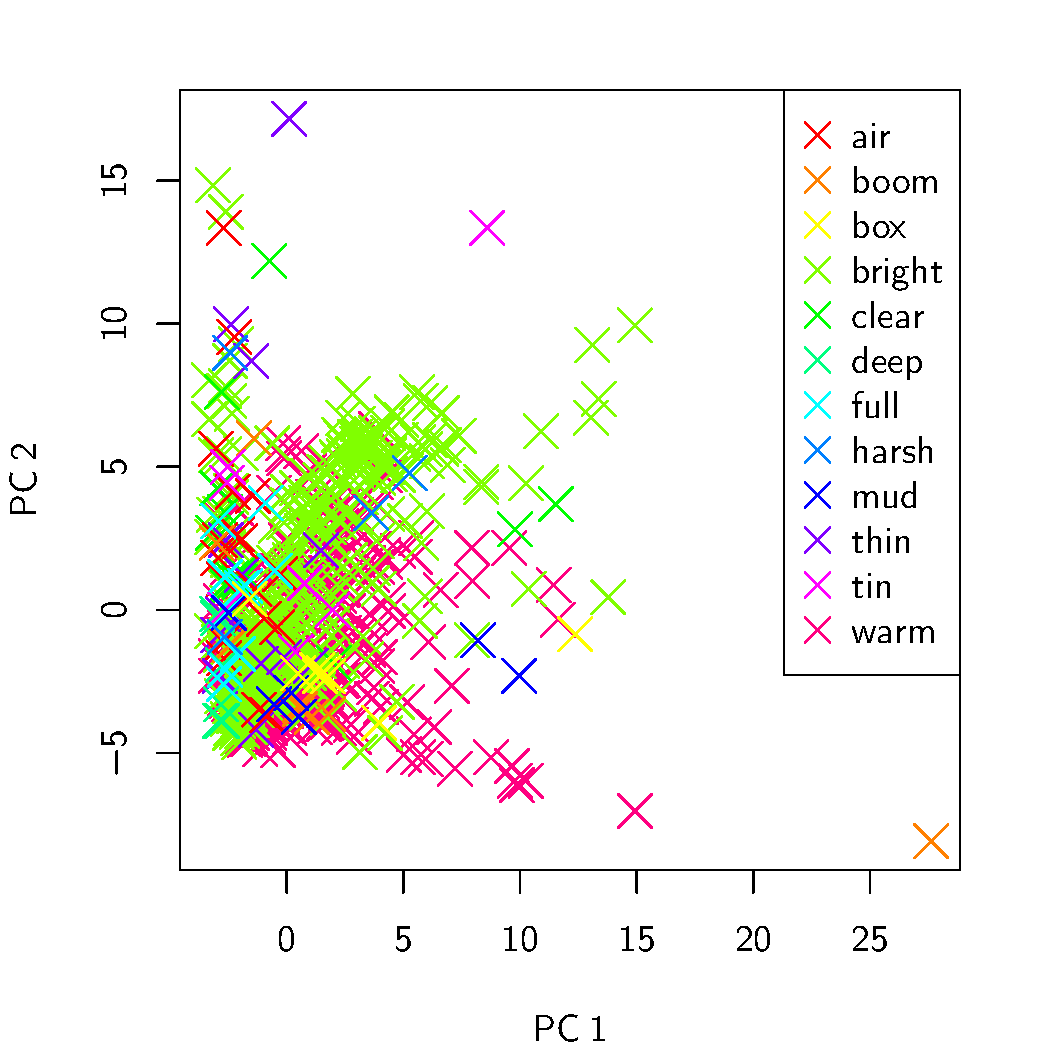
\includegraphics[width=0.45\textwidth]{chapter4/Images/EqualiserProcessedPCA.pdf}
					\label{fig:EqualiserProcessedPCA}
				}
				\qquad
				\subfloat[Descriptor Centroids]
				{
					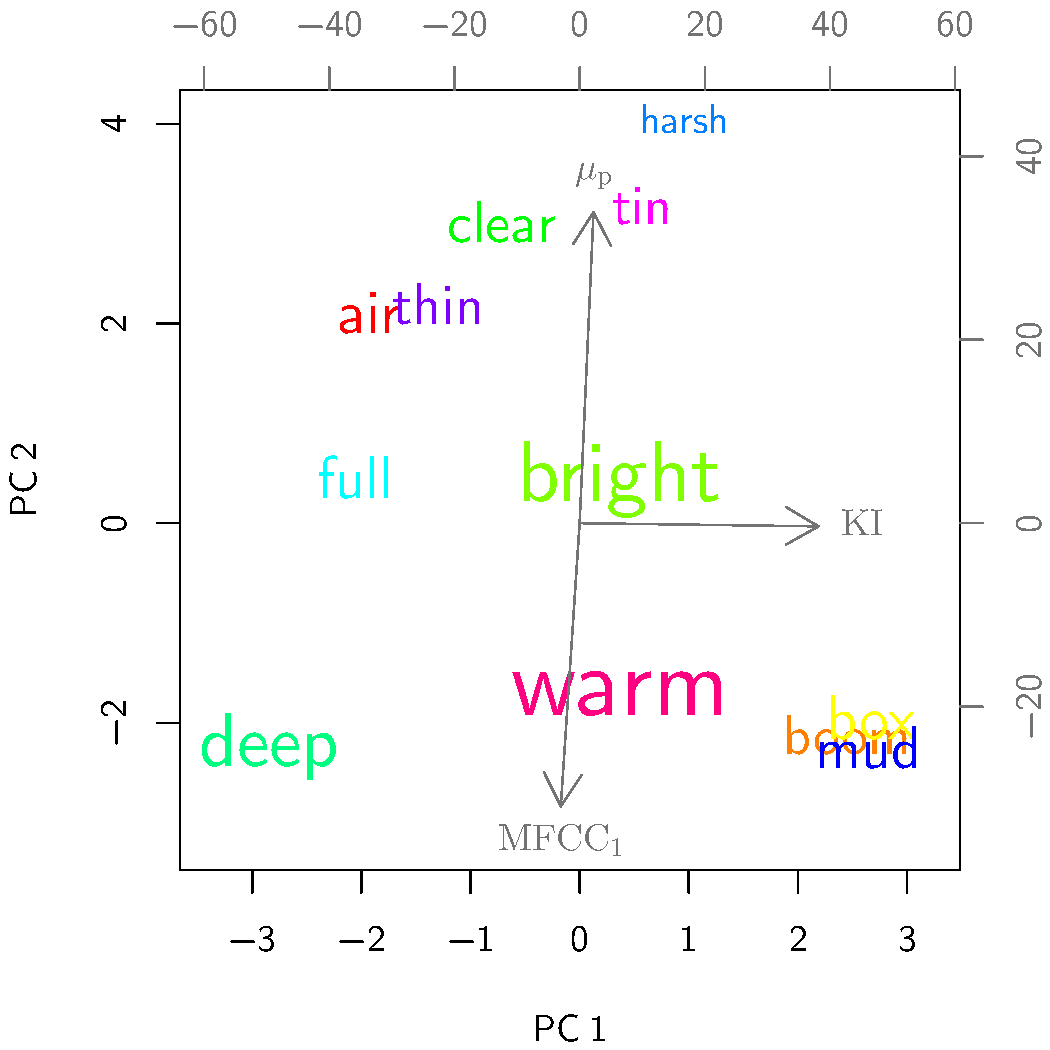
\includegraphics[width=0.45\textwidth]
							{chapter4/Images/EqualiserProcessedCentroidsPCA.pdf}
					\label{fig:EqualiserProcessedCentroidsPCA}
				}
				\caption{Timbre space for the processed features from the equaliser.}
				\label{fig:EqualiserProcessedPCAs}
			\end{figure}

		\subsubsection*{Equaliser Feature Differences}
			\begin{itemize}
				\item {\bf{PC 1:}} $\textrm{KI}$~($p~=~-0.986$), $\textrm{KI}_{\textrm{p}}$~($p~=~-0.970$),
					$\gamma_{\textrm{s}}$~($p~=~-0.968$), $\kappa_{\textrm{p}}$~($p~=~-0.932$),
					$\textrm{KI}_{\textrm{h}}$~($p~=~-0.922$), $\kappa_{\textrm{s}}$~($p~=~-0.915$),
					$\kappa_{\textrm{h}}$~($p~=~-0.912$), $\sigma^{2}$~($p~=~-0.890$),
					$\sigma$~($p~=~-0.872$), $\textrm{RMS}$~($p~=~-0.872$),
					$\gamma_{\textrm{p}}$~($p~=~-0.862$), $\gamma_{\textrm{h}}$~($p~=~-0.831$).
				\item {\bf{PC 2:}} $\mu_{\textrm{p}}$~($p~=~ 0.867$), $\mu_{\textrm{h}}$~($p~=~ 0.863$),
					$\sigma_{\textrm{h}}$~($p~=~ 0.838$), $\sigma_{\textrm{p}}$~($p~=~ 0.833$),
					$\textrm{SRO}$~($p~=~ 0.813$), $\mu_{\textrm{s}}$~($p~=~ 0.770$),
					$\textrm{SSl}$~($p~=~ 0.745$), $\textrm{MFCC}_{1}$~($p~=~-0.705$).
				\item {\bf{PC 3:}} $\textrm{MFCC}_{5}$~($p~=~-0.794$), $\textrm{MFCC}_{6}$~($p~=~-0.791$),
					$\textrm{MFCC}_{7}$~($p~=~-0.741$), $\textrm{MFCC}_{0}$~($p~=~ 0.723$),
					$\textrm{JI}$~($p~=~ 0.722$).
				\item {\bf{PC 4:}} $\textrm{MFCC}_{12}$~($p~=~0.917$), $\textrm{MFCC}_{11}$~($p~=~0.908$),
					$\textrm{MFCC}_{10}$~($p~=~0.893$), $\textrm{MFCC}_{9}$~($p~=~0.848$),
					$\textrm{MFCC}_{8}$~($p~=~0.742$).
			\end{itemize}

			\begin{figure}[h!]
				\centering
				\subfloat[Individual Transforms]
				{
					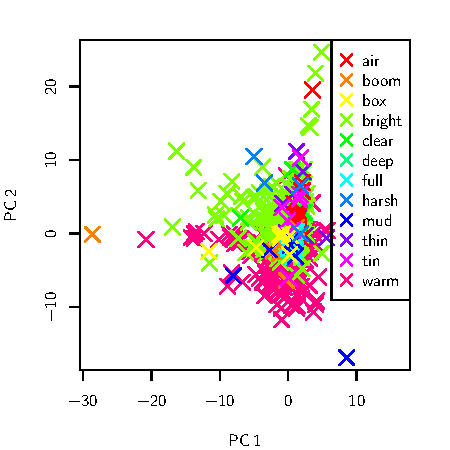
\includegraphics[width=0.45\textwidth]{chapter4/Images/EqualiserDifferencePCA.pdf}
					\label{fig:EqualiserDifferencePCA}
				}
				\qquad
				\subfloat[Descriptor Centroids]
				{
					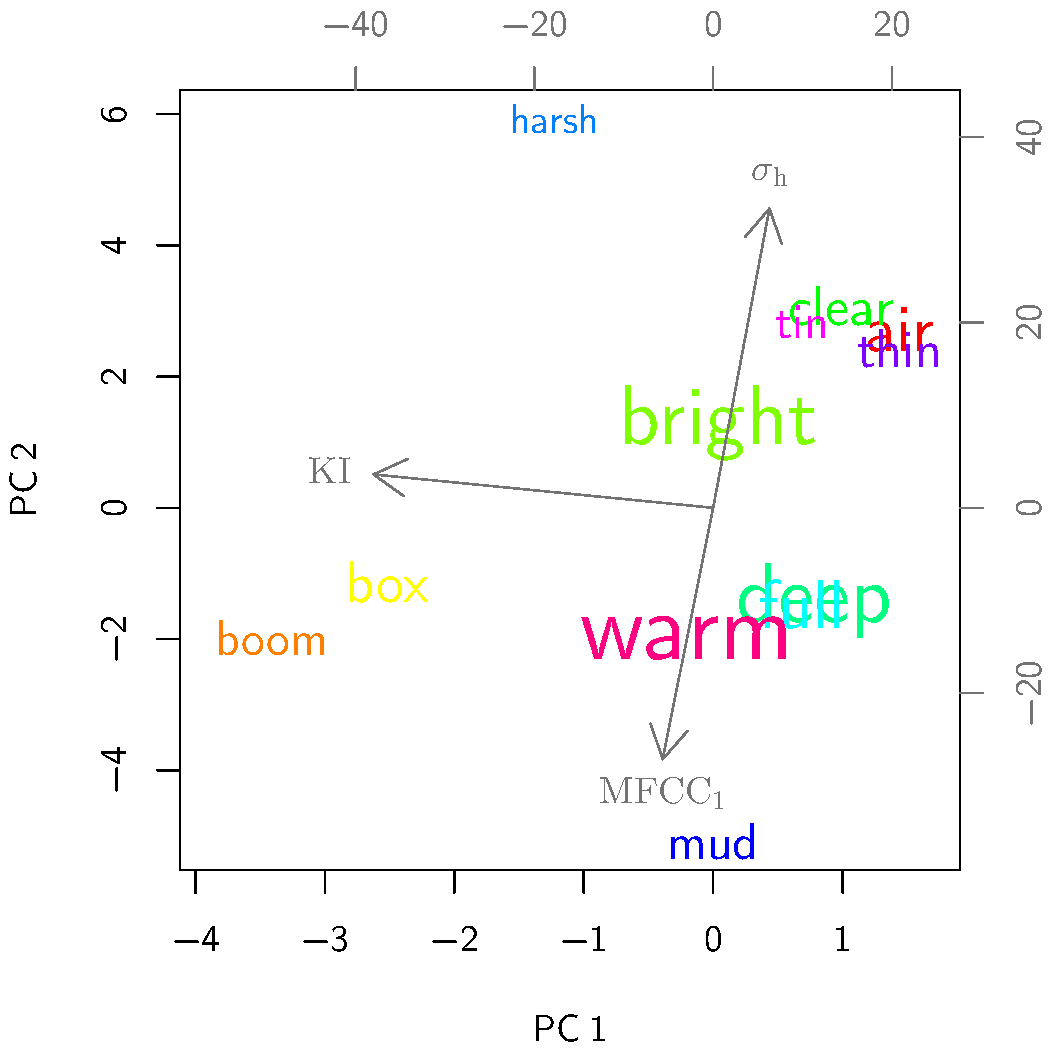
\includegraphics[width=0.45\textwidth]
							{chapter4/Images/EqualiserDifferenceCentroidsPCA.pdf}
					\label{fig:EqualiserDifferenceCentroidsPCA}
				}
				\caption{Timbre space for the feature differences from the equaliser.}
				\label{fig:EqualiserDifferencePCAs}
			\end{figure}

\chapter{Perceptual Listening Test Methodologies}
\label{chap:ListeningTests}
	The systems proposed in Chapter \ref{chap:FeatureControl} provide control over low level features of audio signals.
	As discussed in Chapter \ref{chap:Timbre} these low level features, or combinations of them, contribute to the
	perception of particular semantic features. For this work it is necessary to discover semantic features which are
	identified by the low level features controllable by the systems in Section \ref{sec:FeatureControl-Control}.

	Chapter \ref{chap:Timbre} covered methods used to approach this in the literature. In this section a selection
	of those methods are reviewed for their applicability to this work and a new method is proposed.

\section{Laboratory Listening Tests}
\label{sec:ListeningTests-LaboratoryListeningTests}
	Undertaking subjective listening tests in a laboratory allows the experimenter to control the conditions under which
	the tests are carried out. It can be ensured that the material is presented to each participant via the same
	reproduction equipment, in the same environment, at the same level. This removes any variability in these areas such
	than any perceived differences in the audio samples noted by the participants are due to their perception rather
	than the testing procedure.

	Another advantage of laboratory testing is the ability to screen participants prior to testing. It may be a
	requirement of the experiment that none of the participants have hearing problems. Hearing tests can be carried out
	before the main testing and participants screened accordingly. It is also beneficial that the experimenter is
	typically on hand if a participant is having trouble completing some section of the test.

	\subsection{Multiple Stimuli Tests}
        \label{sec:ListeningTests-LaboratoryListeningTests-MultipleStimuliTests} 
		In a multiple stimuli test participants are presented with several stimuli at once and asked to rate each
		against a given criteria. A multiple stimuli methodology often used in perceptual audio tests is MUSHRA
		(Multiple Stimuli with Hidden Reference and Anchor) \citep{mushra2014}. 

		MUSHRA was developed for grading the quality of lossy audio data compression algorithms. Participants are
		asked to judge how well different systems reconstructed the original signal after lossy data compression.
		These tests are often used to assess the performance of bandwidth extension methods such as those discussed
		in Section \ref{sec:Excitation-Methods}. The listening tests performed in Section
		\ref{sec:FeatureControl-Systems-Individuals} used a similar methodology to that of MUSHRA.

		Other multiple stimulus tests, while not adhering strictly to the MUSHRA guidelines, follow a similar
		structure. \citet{arthi2015influence} uses a multiple stimulus test to determine the perceptual differences
		between samples. This method collects information on the perceptual distances between samples but none on
		how those particular differences are described by the participants.

	\subsection{Verbal Attribute Magnitude Estimation}
	\label{sec:ListeningTests-LaboratoryListeningTests-VAME}
		An overview of VAME methodology was given in Section \ref{sec:Timbre-Parameterisation-AuditoryEvaluation}.
		It is a popular methodology for timbral research as it provides rankings of audio samples against timbral
		descriptors. This not only allows timbre spaces to be constructed but also descriptors to be applied to
		their dimensions as done by \citet{zacharakis2014an}.

		A difficulty encountered when designing a VAME test is the selection of descriptors to use in the tests. As
		discussed by \citet{darke2005assessment} results are not usable if the test participants find it difficult
		to associate a particular descriptor with the audio samples presented.

		In a VAME test the samples are presented to the participants one at a time and rated against several
		criteria. This is in direct opposition to a multiple stimulus test in which the samples are all presented at
		once and rated against a single criteria. VAME tests pose a problem here as there is no reference provided
		against which to rate the samples. Participants must keep several scales (one for each descriptor) in mind
		throughout the duration of the test. This may cause them to use the extremes of the scales too early in the
		test so when presented with a sample they wish to rate closer the extremes they cannot. In a multiple
		stimulus test all the samples are available at once allowing participants to find the samples which lie at
		the extremes and rate the rest accordingly, better utilising the range of the scale.

\section{Distributed Listening Tests}
\label{sec:ListeningTests-DistributedListeningTests}
	While laboratory experiments afford the experimenter the greatest amount of control over the conditions of the
	experiment they can be too restrictive. Typically the experimenter will have limited equipment with which to carry
	out the tests meaning that very few can be run concurrently. For long tests it can be very time consuming to gather
	sufficient data. More recent timbral research has attempted to gather information from a much larger group of
	participants at the loss of control over listening environment. In this section, previous studies methods of doing
	this are discussed and a new method proposed.

	The basic principle underlying all these methods is to distribute the testing software to a wide audience and have
	them carry out the test using their own equipment and return the results. This makes it far easier to collect data
	from a large sample of people as participants are able to take the test at a time which suits them. For laboratory
	tests the participants, experimenter and testing equipment all need to be available at the same time to carry out
	the tests.

	There are several downsides to this type of testing but for certain experiments these may not be as detrimental as
	they first appear. In a laboratory environment the experimenter is present to supervise the tests and ensure that
	participants are able to complete the tasks they are given. With distributed testing no such supervision is given so
	participants which have trouble may produce anomalous results or fail to complete the entire test. These problems
	can be minimised by using a clear testing interface and provision of sufficient documentation / instruction.

	The additional time required for interface design and documentation increases the time taken before testing can
	commence. After this initial investment of time the tests can be run without supervision allowing the experimenter
	to work on other tasks. Once enough data has been collected it can be analysed while additional participants are
	still undertaking the tests. With a well designed experiment researchers can draw conclusions from the first results
	collected while the tests continue to build a larger dataset for further study.

	Lack of control over the listening environment can be a considerable downside for certain listening tests. For
	timbral research this is not so critical if the test can be designed in such a way that effects of the participants
	reproduction equipment have little influence on the results. This influence can never be completely removed but
	steps can be taken to minimise it. One way to reduce the influence is to have participants rate the relative timbral
	difference between samples rather than give absolute ratings on a timbral scale. For this reason multiple stimulus
	style tests are more favorable than VAME tests.

	While the results of the tests will have been influenced by the differences in listening conditions it may lead to
	more easily producible results. The difference in listening conditions will cause higher variance in the data
	reducing the confidence of any correlations found. Any correlations found with sufficiently high confidence however
	will be those which are not affected as much by the reproduction system used. These correlations will then be easier
	to reproduce on other systems leading to a more robust timbral manipulation.

	If the confidence of correlations found in the entire dataset are not high enough the data could be partitioned into
	groups depending on the listening environment the tests were taken in. This allows for the removal of results which
	are causing anomalous results. Perhaps a certain effect in more audible when listening on speakers rather than
	headphones. In order to segment the data in this way additional data should be collected from the test participants.
	\citet{wilmering2013audio} have participants select an option from a drop down list which best describes their
	listening environment prior to beginning the test. They find that there was not much variance between the results
	across the different groups although the majority of the participants assigned themselves to the same group.

	\citet{seetharaman2014crowdsourcing} prompt participants for information about their listing environment but also
	include an extra testing section to ensure a participants reproduction system is suitable for the tests. This extra
	section assesses the range of frequencies a participants system can reproduce and excludes those which do not meet
	the required criteria.
	
	\subsection{Web Based Testing}
	\label{sec:ListeningTests-DistributedListeningTests-Web}
		A popular method of distributing listening tests is to build a web interface in which the testing is carried
		out \citep{wilmering2013audio, cartwright2013socialeq, seetharaman2014crowdsourcing}. Using a web interface
		for testing allows subjects to participate from wherever they can access the internet. An advantage of using
		a web interface is that participants do not need to download any software specific to the test. This may see
		the participation of people who otherwise would have been dissuaded due to not wanting to download untrusted
		software.

		A disadvantage of a web implementation is the limitations of audio processing in web browsers. Simple
		interfaces which involve playback of audio samples are easily implemented but more complex audio processing
		and multiple channel audio playback are still difficult. This is becoming more possible due to development
		of the web audio API \citep{adenot2015web}, although not all the features of this are currently supported by
		all web browsers reducing the potential audience for the test.

		An extension of web based testing is to create an interface for mobile platforms. The Tunebot project
		\citep{huq2010crowdsourcing} has multiple interfaces to its sever side back end. Having multiple interfaces
		increases the number of people who will be able to participate in the testing.

		\note
		{
			Gamification of listening tests in order to entice more people to contribute.
		}

	\subsection{DAW Based Timbre Evaluation} % this name will probably change
	\label{sec:ListeningTests-DistributedListeningTests-DAWBasedTimbreEvaluation}
		The previously discussed testing methodologies all rely on the participants performing a certain set of
		tasks. While this structure helps to reduce the number of variables in an experiment it does not necessarily
		reflect the way audio is treated in a production environment.

		A new methodology has been developed in which the analysis of timbre is introduced into a typical music
		production workflow causing minimal interruption to the producer. This methodology aims to answer the
		question "What terms do music producers use to describe the timbral transformations they apply to audio
		during the creation of music?". 
		
		This section will detail what the typical production workflow is and how semantic information can be
		gathered.

		\subsubsection{Music Production Workflow}
			\todo{Find some references for this section. Probably mixing engineers handbook or something.}

			The music production workflow has four main stages:

			\begin{itemize}
				\item Recording
				\item Editing
				\item Mixing
				\item Mastering
			\end{itemize}

			At every stage of this process semantic descriptors are often used to communicate the desired
			timbral qualities of the audio. For instance one my ask that a certain microphone be used because of
			the `warmth' it adds to the recorded sound. During the mixing and mastering stages audio processing
			effects are applied to shape the timbre further.  These stages will be the focus of this section as
			the aim of this thesis is to improve the intuitiveness of these effects.

			Historically audio effects were pieces of electronic hardware through which an audio signal is
			passed. Modern music production techniques utilise Digital Audio Workstation (DAW) software. This
			software enables users to record, edit and mix multiple tracks of audio using a computer. 
			
		\subsubsection{Analysis of Timbre Inside the DAW}
			An ideal way to collect timbral information during music production would be to have the DAW analyse
			the audio tracks used and production techniques applied. Information which could be gathered
			directly from the DAW, with no extra input from the user, includes:

			\begin{itemize}
				\item Information about the audio processing chain:
				\begin{itemize}
					\item The effects applied to each track.
					\item The order in which these effects are applied.
					\item The parameter settings of these effects.
				\end{itemize}

				\item Features of the audio at every stage in the processing chain.
			\end{itemize}

			Additional information can be gathered by prompting the user for input:

			\begin{itemize}
				\item The genre of music being produced.
				\item The content of the separate audio tracks (what instruments etc.).
				\item Semantic terms which describe the timbral transformations applied by each audio
					effect.
			\end{itemize}

			Achieving this would require the creation of a new DAW. This would be impractical for the current
			research. DAWs are very comprehensive software packages which perform many more tasks than the
			application of effects to audio (project management, audio editing functionality etc.). A lot of
			effort would be expended in implementing these features before any timbral data could be collected.
			Music producers also tend to have a preferred DAW with which they work most fluidly. Convincing
			producers to use a new DAW, for the purposes of research, would be a difficult task.

			Third party developers can produce extensions to DAWs known as plug-ins. Plug-Ins provide additional
			audio processing functionality to the DAW environment. They can optionally expose their own
			parameters which users can adjust to achieve their desired effect. There are several different
			formats in which audio plug-ins can be distributed (VST, AU etc.). Most of the commonly used DAWs
			support plug-ins in one or more of these formats.

			Audio plug-ins provide a good platform to allow producers to provide semantic terms and audio
			feature information from within their preferred DAW. As part of this research a suite of audio
			plug-ins which extract this information have been developed. They have been release under the title
			Semantic Audio Feature Extraction (SAFE) Plug-Ins.

		\subsubsection{SAFE Plug-Ins}
			The SAFE plug-ins consist of four commonly used audio effects: Equaliser, Distortion, Compressor and
			Reverb. As part of the plug-ins's interface the user has the option to save semantic terms. The
			interface for the SAFE Distortion is shown in Figure \ref{fig:SAFE-Distortion}. Upon saving terms
			the plug-in will analyse the audio at its inputs and outputs. When the analysis is completed the
			results are stored, containing:

			\begin{itemize}
				\item The users description of the timbre.
				\item The plug-in's current parameter settings.
				\item The features of the audio before and after processing.
				\item Some additional data about the user and the track being worked on.
				\begin{itemize}
					\item The genre.
					\item The instrument.
					\item The users age.
					\item The users location.
					\item The users primary language.
					\item The number of year experience the user has in music production.
				\end{itemize}
			\end{itemize}

			\begin{figure}[h!]
				\centering
				\includegraphics[width=0.8\textwidth]{chapter5/Images/SAFEDistortion.png}
				\caption{The Interface for the SAFE Distortion Plug-In}
				\label{fig:SAFE-Distortion}
			\end{figure}

			The LibXtract library \citep{bullock2007libxtract} is used in the analysis of the audio. Every
			scalar feature available within LibXtract is calculated along with the MFCCs and Bark Band
			Coefficients. In total five seconds of audio is analysed in frames of 4096 samples each.

			\note{Why 4096 samples? The real reason is because LibXtract works better that way. Will that cut
			the mustard?}

			One disadvantage in using plug-ins is that they cannot gather information about the rest of the
			processing chain they may be a part of. The timbral transformation the user is describing my be the
			result of several effects working together. This can be mitigated somewhat by asking users to
			describe only the effect the plug-in in question is providing.

			The SAFE plug-ins also suffer from the same issues other distributed tests do. The researcher
			forfeits control over the listening environment in order to gather results from a much larger sample
			of people. In fact the they provide even lest control that methodologies like that used in the
			Social EQ project \citep{cartwright2013socialeq} in that the choice of audio samples being used is
			decided by the test subject. 

%Suitability of Exciters for Perceptual Control
%	Parameterise feature changes in terms of harmonic excitation.
%	Most suitable methods for given feature manipulations.
%	Easiest features to control in isolation.

\chapter{Controlling Audio Features} % control of low level features using exciters
\label{chap:FeatureControl}

\section{Introduction}
\label{sec:FeatureControl-Introduction}
	As discussed in Section \ref{sec:Timbre-Control}, previous studies have attempted to control perceptual features by
	controlling specific audio features. This chapter will identify the audio features which can be controlled through
	harmonic excitation and which excitation algorithms are the most suitable for given feature changes. Firstly, in
	Section \ref{sec:FeatureControl-Systems}, various challenges which arise when building harmonic excitation systems
	are discussed and methods to counteract them are suggested. A number of different systems are proposed which
	provide control over the nature of the new frequency components introduced to the signal. In Section
	\ref{sec:FeatureControl-Parameterisation} methods by which these systems can be configured to control specific
	audio features are proposed and tested.

\section{Harmonic Excitation Systems}
\label{sec:FeatureControl-Systems}
	In Section \ref{sec:Excitation-Methods} several different methods of introducing new frequency content to a signal
	were introduced. In Section \ref{sec:ExcitationEvaluation-Comparison} these methods were discussed further and the
	degree to which their effect can be controlled evaluated. From that analysis this is know that better control over
	the output is gained through meeting certain input requirements, for instance the SSBA and IAP techniques will
	produce sinusoidal outputs for sinusoidal inputs. It is also noted that further filtering may be needed after the
	use of a harmonic excitation algorithms in order to shape the spectrum as desired, such as after a peak clipper has
	been applied. Harmonic excitation systems can be constructed which apply these pre and post-processing before and
	after a giver harmonic excitation algorithm. This section discusses the design of these systems, aiming to give
	users precise control over the new spectral content added to a wide range of input signals.

	\subsection{$f_{0}$ Tracking}
	\label{sec:FeatureControl-Systems-Fundamental}
		The majority of the methods discussed in Section \ref{sec:Excitation-Methods} will cause intermodulation
		distortion when used on signals with multiple frequency components. As the effects of this intermodulation
		distortion can be difficult to predict it can be useful to eliminate it altogether. This should make the
		effects of a system more predictable allowing it to be used in more situations.	Intermodulation distortion
		can be reduced by reducing the number of frequency components in the input signal. For a sinusoidal input
		(one frequency component) no intermodulation distortion occurs. The intermodulation introduced by a
		harmonic excitation system can then be reduced by pre-processing a signal to make it as sinusoidal as
		possible. This can be achieved by only processing the $f_{0}$ of a signal, the $f_{0}$ can be isolated with
		a filter producing a narrowband signal with the majority of its energy concentrated at the $f_{0}$. In the
		following discussion this filtered signal will be referred to as the `isolated $f_{0}$'. Applying a
		harmonic excitation algorithm to the isolated $f_{0}$ will produce a signal with a lower level of
		intermodulation components than processing the original input signal. The `excited' isolated $f_{0}$ signal
		can then be summed with the original signal to produce the output. A diagram of this system is shown in
		Figure \ref{fig:F0Tracking}.

		\begin{figure}[h!]
			\centering
			\begin{tikzpicture}
				\node (In) at (0, 1) {$x[n]$};
				\coordinate (InMid) at (1, 1);
				\draw (In) -- (InMid);

				\coordinate (Through) at (1, 0);
				\draw (InMid) -- (Through);
				\coordinate (ThroughOut) at (9, 0);
				\draw (Through) -- (ThroughOut);

				\coordinate (Side) at (1, 2);
				\draw (InMid) -- (Side);

				\node (F0) [draw] at (2.5, 2) {$f_{0}$ Tracker};
				\node (Filter) [draw] at (2.5, 1) {LPF};
				\draw (InMid) -- (Filter);
				\draw (F0) -- (Filter);

				\node (Exciter) [draw] at (5, 1) {Harmonic Exciter};
				\draw (Filter) -- (Exciter);
				\draw (Side) -- (F0);

				\node (Add) [operator] at (9, 1) {+};
				\draw (ThroughOut) -- (Add);

				\node (Gain) [gain] at (7.5, 1) {Gain};
				\draw (Exciter) -- (Gain);
				\draw (Gain) -- (Add);

				\node (Out) at (10.25, 1) {$y[n]$};
				\draw (Add) -- (Out);
			\end{tikzpicture}
			\caption{$f_{0}$ frequency tracking in a harmonic excitation system.}
			\label{fig:F0Tracking}
		\end{figure}

		For this system to operate in real time the $f_{0}$ of the signal must be calculated in real time. This is
		achieved using the $f_{0}$ tracker shown in the diagram. $f_{0}$ tracking is a widely researched field and
		several algorithms have been presented in the literature, several of which are reviewed by
		\citet{cuadra2001efficient} and \citet{gerhard2003pitch}.  $f_{0}$ tracking can be done in both the time
		and frequency domains. The simplest method being to count the number of instances of a particular event in
		a given time period. This even could be a zero crossing or a peak or any other easily identifiable feature
		of the signal. As signals get more complex this method becomes more difficult to apply as higher frequency
		content will produce more instances of the event being counted. More advanced time domain methods include
		the Average Magnitude Difference Function (AMDF) and autocorrelation methods. Many modern $f_{0}$ tracking
		systems are based on these, such as the VT-AMDF algorithm proposed by \citet{prukkanon2009vt-amdf}.  These
		methods require frame based processing which reduces the time resolution of the system. If analysing real
		time audio the current estimate of the $f_{0}$ will lag behind the audio signal.  \citet{larsen2004audio}
		describe a time domain frequency tracker which uses a simple recursive formula. While this is not as
		precise as the more advanced techniques it takes considerably less time to compute. Frequency domain
		methods require the DFT of the signal to be calculated introducing considerable complexity. Widely used
		frequency domain techniques include the Harmonic Product Spectrum (HPS) and maximum likelihood
		estimate methods \citep{noll1969pitch}.

		For real time harmonic excitation, the accuracy of the $f_{0}$ tracking algorithm is not as important as it
		is in other fields such as automatic music transcription. The aim of the system in Figure
		\ref{fig:F0Tracking} is to reduce the level of higher harmonics compared to the $f_{0}$. Using a low pass
		filter with a cutoff frequency close to the $f_{0}$ will achieve this. The lag between the audio and the
		estimate of the $f_{0}$ is of greater concern. The system needs to respond quickly to changes in $f_{0}$ in
		order to better isolate it for processing.

		A problem is posed by signals with little energy at their $f_{0}$, such as those produced in the lower
		register of a Double Bass \citep{askenfelt2010double}. An $f_{0}$ tracking algorithm will still return the
		frequency of the $f_{0}$ despite its low magnitude. The isolated $f_{0}$ may then have too little amplitude
		to be of any use for harmonic excitation. A frequency domain approach to $f_{0}$ tracking may be more
		robust in this situation as it is easier to check whether there is sufficient energy at the detected
		$f_{0}$. If there is not, the first harmonic which has sufficient magnitude can be isolated and used as the
		input to the exciter. If this action is taken, only the spectral replication and spectral shifting methods
		will allow for the excitation of every harmonic. The SSBA and IAP methods only allow for integer
		multiplications of the input frequency.

		The system shown in Figure \ref{fig:F0Tracking} can provide differing levels of flexibility depending on
		the harmonic exciter used. Using a simple clipper will generate a series of harmonics of the $f_{0}$. Using
		methods which provide more control over the order of distortion allows users to excite single harmonics in
		the output. This will be covered in the next section.

	\subsection{Individual Harmonic Generation}
	\label{sec:FeatureControl-Systems-Individuals}
		Control over which harmonics are excited in a signal can be achieved by generating individual harmonics.
		The principle behind this is to isolate the $f_{0}$ and then shift its frequency to that of the desired
		harmonic, as done in the system shown in Figure \ref{fig:HarmonicGenerationSystem}.  The frequency shifter
		in this system can be implemented the SSBA, IAP, Spectral Replication or Spectral Stretching methods.

		\begin{figure}[h!]
			\centering
			\begin{tikzpicture}
				\node (In) at (0, 1) {$x[n]$};
				\coordinate (InMid) at (1, 1);
				\draw (In) -- (InMid);

				\coordinate (Side) at (1, 2);
				\draw (InMid) -- (Side);

				\node (F0) [draw] at (2.5, 2) {$f_{0}$ Tracker};
				\node (Filter) [draw] at (2.5, 1) {LPF};
				\draw (InMid) -- (Filter);
				\draw (F0) -- (Filter);

				\node (Exciter) [draw] at (5, 1) {Frequency Shifter};
				\draw (Filter) -- (Exciter);
				\draw (Side) -- (F0);

				\node (Out) at (7.25, 1) {$y[n]$};
				\draw (Exciter) -- (Out);
			\end{tikzpicture}
			\caption{Generating individual harmonics for a signal.}
			\label{fig:HarmonicGenerationSystem}
		\end{figure}

		A complex spectrum can be created by generating several different order harmonics in this manner and
		summing them together. \citet{bregman1994auditory} suggests that when presented with an auditory scene the
		human hearing system separates out sources by grouping like harmonics together. Whether harmonics are
		deemed to be similar depends on their frequency and amplitude envelopes. When applying harmonic excitation
		it is necessary to ensure that the newly introduced harmonic content will be judged as similar to the
		existing content. If not, the excited harmonics may be perceived as a new sound source rather than
		contributing towards changing the timbre of a sound. Any system which generates new harmonic content and
		then sums it back into the original signal is at risk of this occurring. When generating multiple harmonics
		individually and summing them all together this risk is increased. Minimising the number of individual
		harmonics generated limits the problems arising from this as well as decreasing the computational load. The
		following section discusses how a system can be constructed which provides sufficient control over the
		shape of a spectrum while limiting the number of harmonics generated individually.
		
	\subsection{Spectral Shaping}
	\label{sec:FeatureControl-Systems-SpectralShaping}
		As seen in Section \ref{sec:ExcitationEvaluation-Comparison-SpectralCharacteristics}, static nonlinearities
		provide an efficient way to generate large numbers of harmonics for sinusoidal inputs. The characteristic
		curve of the nonlinearity can be designed to produce a set of harmonics with the desired qualities, the
		parity of the characteristic curve can be used to control whether odd or even harmonics are generated and
		the `smoothness' of the curve can be adjusted to control the roll off of the harmonics' amplitudes. The
		shape of the generated spectrum can then be further shaped by filtering.

		A spectral shaping system can be constructed in which a static nonlinearity and filter are used to excite a
		large band of harmonics and finer control is provided using the individual harmonic generation method shown
		in Figure \ref{fig:HarmonicGenerationSystem}. This allows the majority of the harmonics to be excited in
		an efficient manner, only using more complex processing where it is needed. \citet{howard2009acoustics}
		discusses how low order harmonics sit in separate critical bands, whereas high order harmonics are within
		one critical bandwidth of one another. This means that lower order harmonics are resolved separately by the
		human hearing system, while the high order harmonics are perceived as fused sounds. As the order of
		harmonics increases, their individual amplitudes have less effect on the perceived timbre of the sound. For
		this reason, a harmonic excitation system need only provide control over the individual amplitudes of low
		order harmonics. 

		Using Equation \ref{eq:ERB}, the minimum order for which harmonics lie within one critical bandwidth of one
		another can be calculated. For a signal with a given $f_{0}$, this order, $n$, can be calculated using the
		inequality in Equation \ref{eq:MinimumFusedHarmonic}.

		\begin{gather}
			f_{0} < 24.7 \left( 4.37n \frac{f_{0}}{1000} + 1 \right) \nonumber \\
			n > 1000 \frac{f_{0} - 24.7}{24.7 \times 4.37f_{0}}
			\label{eq:MinimumFusedHarmonic}
		\end{gather}

		This value is dependant on the $f_{0}$ of the signal. As $f_{0}$ rises, the minimum value of $n$ grows
		asymptotically towards 9.26 as shown in Equation \ref{eq:IndividualHarmonicLimit}.

		\begin{equation}
			\lim_{f_{0} \to \infty} 1000 \frac{f_{0} - 24.7}{24.7 \times 4.37f_{0}} \approx 9.26
			\label{eq:IndividualHarmonicLimit}
		\end{equation}

		For any value of $f_{0}$, a maximum of nine harmonics will lie at least one critical bandwidth away from
		all other harmonics. The individual amplitudes of the tenth, and higher order, harmonics have less effect
		on the timbre of a signal. This leads to the system shown in Figure \ref{fig:SpectralShapingSystem}, an
		expansion of the system shown in Figure \ref{fig:F0Tracking} providing finer control over the amplitudes of
		the first nine harmonics. The $f_{0}$ is isolated in the same manner but several exciters are used in
		parallel. Each of the first nine harmonics are generated individually from the isolated $f_{0}$. Higher
		order harmonics are generated using a static nonlinearity and high pass filter in combination. The filter's
		primary purpose is to remove any energy present in the first nine harmonics but can also be used to alter
		the distribution of energy in the higher order harmonics.

		\begin{figure}[h!]
			\centering
			\begin{tikzpicture}
				\node (In) at (-1, -1.75) {$x[n]$};
				\coordinate (InMid) at (0, -1.75);
				\draw (In) -- (InMid);

				\coordinate (Side) at (0, -0.75);
				\draw (InMid) -- (Side);

				\node (F0) [draw] at (2, -0.75) {$f_{0}$ Tracker};
				\node (F0Filter) [draw] at (2, -1.75) {LPF};
				\draw (InMid) -- (F0Filter);
				\draw (F0) -- (F0Filter);
				\draw (Side) -- (F0);

				\node (Add) [operator] at (10.5, -1.75) {+};

				\coordinate (ExciterIn) at (4, -1.75);
				\draw (F0Filter) -- (ExciterIn);

				% the fundamental
				\coordinate (F0In) at (4, 1);
				\node (F0Gain) [gain] at (9, 1) {};
				\draw (F0In) -- (F0Gain);
				\coordinate (F0Out) at (9.5, 1);
				\draw (F0Gain) -- (F0Out);
				\draw (F0Out) -- (Add);

				% second harmonic
				\coordinate (F1In) at (4, 0);
				\draw (F0In) -- (F1In);
				\node (F1) [draw] at (6.5, 0) {2\super{nd} Harmonic};
				\draw (F1In) -- (F1);

				\node (F1Gain) [gain] at (9, 0) {};
				\draw (F1) -- (F1Gain);
				\coordinate (F1Out) at (9.5, 0);
				\draw (F1Gain) -- (F1Out);
				\draw (F1Out) -- (Add);

				% third harmonic
				\coordinate (F2In) at (4, -1);
				\draw (F1In) -- (F2In);
				\node (F2) [draw] at (6.5, -1) {3\super{rd} Harmonic};
				\draw (F2In) -- (F2);

				\node (F2Gain) [gain] at (9, -1) {};
				\draw (F2) -- (F2Gain);
				\coordinate (F2Out) at (9.5, -1);
				\draw (F2Gain) -- (F2Out);
				\draw (F2Out) -- (Add);

				% ninth harmonic
				\coordinate (F8In) at (4, -2.5);
				\draw (F2In) -- (F8In);
				\node (F8) [draw] at (6.5, -2.5) {9\super{th} Harmonic};
				\draw (F8In) -- (F8);

				\node (F8Gain) [gain] at (9, -2.5) {};
				\draw (F8) -- (F8Gain);
				\coordinate (F8Out) at (9.5, -2.5);
				\draw (F8Gain) -- (F8Out);
				\draw (F8Out) -- (Add);

				\draw [dots] (F2) -- (F8);
				\draw [dots] (F2Gain) -- (F8Gain);

				% high order harmonics
				\coordinate (HighIn) at (4, -3.5);
				\draw (F8In) -- (HighIn);
				\node (High) [draw] at (5.7, -3.5) {Nonlinear Device};
				\draw (HighIn) -- (High);

				\node (HighFilter) [draw] at (8, -3.5) {Filter};
				\draw (High) -- (HighFilter);

				\node (HighGain) [gain] at (9, -3.5) {};
				\draw (HighFilter) -- (HighGain);
				\coordinate (HighOut) at (9.5, -3.5);
				\draw (HighGain) -- (HighOut);
				\draw (HighOut) -- (Add);

				% through
				\coordinate (Through) at (0, -4.5);
				\draw (InMid) -- (Through);
				\node (ThroughGain) [gain] at (9, -4.5) {};
				\draw (Through) -- (ThroughGain);
				\coordinate (ThroughOut) at (9.5, -4.5);
				\draw (ThroughGain) -- (ThroughOut);
				\draw (ThroughOut) -- (Add);

				\node (Out) at (11.75, -1.75) {$y[n]$};
				\draw (Add) -- (Out);
			\end{tikzpicture}
			\caption{An excitation system for controlling spectral structure.}
			\label{fig:SpectralShapingSystem}
		\end{figure}

	\subsection{Superposition}
	\label{sec:FeatureControl-Systems-Superposition}
		When processing musical signals, additional challenges are met when attempting to shape the spectrum
		through excitation. One such challenge concerns the superposition of the existing harmonics in a signal and
		those produced by the excitation. In certain situations these two signals may cause destructive
		interference. Although the exciter is set to produce energy at a given harmonic, when the signals are
		summed the energy at this harmonic decreases. To calculate the final amplitude of a harmonic, after the
		excited signals have been summed with the original signal, the phases and amplitudes of that harmonic in
		the original and excited signals must be known. This involves performing a full spectral analysis on the
		input signal. 

		When using a system like that shown in Figure \ref{fig:SpectralShapingSystem}, the phases and amplitudes of
		the excited harmonics depend on the phase and amplitude of the isolated $f_{0}$. Using the SSBA and IAP
		techniques to generate the $n$\super{th} harmonic, the phase of the output is $n$ times that of the input
		after the Hilbert transform filter has been applied. The phases of the harmonics produced by a static
		nonlinearity can be determined by calculating the Fourier series of a sinusoid with the nonlinearity
		applied. Calculating this in real time dramatically increases the computational complexity of the system.
		This complexity can be avoided by avoiding superposition of harmonics. This simplest way to achieve this is
		by discarding the original signal and constructing the output from only the $f_{0}$ and generated
		harmonics.  This destroys most of the timbral characteristics of a signal, completely reconstructing its
		spectrum. For situations where a dramatic alteration of timbre is desired this can be a useful technique
		but for more subtle timbral manipulations it is better to preserve more of the original spectral structure.

		A less intrusive method is to filter energy out of the input signal only at the frequencies which are to be
		excited. For the system in Figure \ref{fig:SpectralShapingSystem} this can be implemented using a series of
		notch filters tuned to the frequencies of the first nine harmonics and a low pass filter to attenuate any
		frequency above the ninth harmonic. These filters can be applied to the unexcited signal depending on which
		harmonics are being generated by the exciters. A diagram of a system which includes these filters is shown
		in Figure \ref{fig:SuperpositionSystem}.

		\begin{figure}[h!]
			\centering
			\begin{tikzpicture}
				\node (In) at (-1, -1.75) {$x[n]$};
				\coordinate (InMid) at (0, -1.75);
				\draw (In) -- (InMid);

				\coordinate (Side) at (0, -0.75);
				\draw (InMid) -- (Side);

				\node (F0) [draw] at (2, -0.75) {$f_{0}$ Tracker};
				\node (F0Filter) [draw] at (2, -1.75) {LPF};
				\draw (InMid) -- (F0Filter);
				\draw (F0) -- (F0Filter);
				\draw (Side) -- (F0);

				\node (Add) [operator] at (10.5, -1.75) {+};

				\coordinate (ExciterIn) at (4, -1.75);
				\draw (F0Filter) -- (ExciterIn);

				% the fundamental
				\coordinate (F0In) at (4, 1);
				\node (F0Gain) [gain] at (9, 1) {};
				\draw (F0In) -- (F0Gain);
				\coordinate (F0Out) at (9.5, 1);
				\draw (F0Gain) -- (F0Out);
				\draw (F0Out) -- (Add);

				% second harmonic
				\coordinate (F1In) at (4, 0);
				\draw (F0In) -- (F1In);
				\node (F1) [draw] at (6.5, 0) {2\super{nd} Harmonic};
				\draw (F1In) -- (F1);

				\node (F1Gain) [gain] at (9, 0) {};
				\draw (F1) -- (F1Gain);
				\coordinate (F1Out) at (9.5, 0);
				\draw (F1Gain) -- (F1Out);
				\draw (F1Out) -- (Add);

				% third harmonic
				\coordinate (F2In) at (4, -1);
				\draw (F1In) -- (F2In);
				\node (F2) [draw] at (6.5, -1) {3\super{rd} Harmonic};
				\draw (F2In) -- (F2);

				\node (F2Gain) [gain] at (9, -1) {};
				\draw (F2) -- (F2Gain);
				\coordinate (F2Out) at (9.5, -1);
				\draw (F2Gain) -- (F2Out);
				\draw (F2Out) -- (Add);

				% ninth harmonic
				\coordinate (F8In) at (4, -2.5);
				\draw (F2In) -- (F8In);
				\node (F8) [draw] at (6.5, -2.5) {9\super{th} Harmonic};
				\draw (F8In) -- (F8);

				\node (F8Gain) [gain] at (9, -2.5) {};
				\draw (F8) -- (F8Gain);
				\coordinate (F8Out) at (9.5, -2.5);
				\draw (F8Gain) -- (F8Out);
				\draw (F8Out) -- (Add);

				\draw [dots] (F2) -- (F8);
				\draw [dots] (F2Gain) -- (F8Gain);

				% high order harmonics
				\coordinate (HighIn) at (4, -3.5);
				\draw (F8In) -- (HighIn);
				\node (High) [draw] at (5.7, -3.5) {Nonlinear Device};
				\draw (HighIn) -- (High);

				\node (HighFilter) [draw] at (8, -3.5) {Filter};
				\draw (High) -- (HighFilter);

				\node (HighGain) [gain] at (9, -3.5) {};
				\draw (HighFilter) -- (HighGain);
				\coordinate (HighOut) at (9.5, -3.5);
				\draw (HighGain) -- (HighOut);
				\draw (HighOut) -- (Add);

				% through
				\coordinate (Through) at (0, -4.5);
				\draw (InMid) -- (Through);
				\node (ThroughFilter) [draw] at (8, -4.5) {Filter};
				\draw (Through) -- (ThroughFilter);
				\node (ThroughGain) [gain] at (9, -4.5) {};
				\draw (ThroughFilter) -- (ThroughGain);
				\coordinate (ThroughOut) at (9.5, -4.5);
				\draw (ThroughGain) -- (ThroughOut);
				\draw (ThroughOut) -- (Add);

				\node (Out) at (11.75, -1.75) {$y[n]$};
				\draw (Add) -- (Out);
			\end{tikzpicture}
			\caption{The system from Figure \ref{fig:SpectralShapingSystem} extended to allow for filtering of
				 the original signal.}
			\label{fig:SuperpositionSystem}
		\end{figure}

		Removing harmonics from the original signal looses any phase information that was present for those
		frequencies. The newly generated harmonics may not have the same phase as those that have been removed,
		potentially causing unwanted timbral effects. The phases of a signal's partials influence its temporal
		features. \citet{plomp1969effect} discuss the audible effects of this for harmonic signals, concluding that
		the effect is more subtle than, but independent to, that of changing the harmonics' amplitudes. They state
		that the largest perceptual difference occurs between a signal in which all the harmonics have the same
		phase and one composed of harmonics with phases alternating between two values $\frac{\pi}{2}$ radians
		apart.

		For fine control it may be beneficial to separate control of the amplitude and phase of each partial in a
		signal. This is most easily achieved using the IAP technique as the phase of the input signal is already
		exposed in the calculation. Introducing a phase parameter, $\theta$, to Equation \ref{eq:IAP} gives rise to
		Equation \ref{eq:IAPWithPhase}. Assuming a sinusoidal input this new parameter controls the phase of the
		generated harmonic relative to that of the input. 

		\begin{equation}
			y[n] = \abs{x_{a}[n]} \cos \left( h\arg(x_{a}[n] + \theta) \right), \quad h \in \textbf{N}
			\label{eq:IAPWithPhase}
		\end{equation}

		For introducing new spectral content with a specific amplitude and phase Equation \ref{eq:IAPWithPhase}
		suffices. Separate control of the phase and amplitudes of existing partials can be achieved in two ways.
		The first is to use an analysis / resynthesis system in which the amplitudes and phases of the partials are
		adjusted in the frequency domain. The second approach is to use zero phase filters to amplify or attenuate
		partials and phase shifting techniques to adjust their phases. Both of these approaches introduce delay
		into the system, be it through the windowing used for spectral analysis or the delay introduced in applying
		zero phase filters.

	\subsection{Inharmonicity}
	\label{sec:FeatureControl-Systems-Inharmonicity}
		With a sinusoidal input the SSBA and IAP techniques generate perfectly harmonic partials. As inharmonicity
		is an important cue for differentiating timbre it is desirable to be able to introduce some inharmonicity
		to the generated partials. Spectral replication allows for generation of partials at any frequency, but in
		order for their frequency to be precise the exact $f_{0}$ must be known. This causes the system to rely on
		the accuracy of the $f_{0}$ tracking algorithm used, meaning a much more complex tracker needs to be used,
		adding to the complexity of the system. A system which provides control over inharmonicity and does not
		rely on precise $f_{0}$ tracking is shown in Figure \ref{fig:InharmonicitySystem}.

		\begin{figure}[h!]
			\centering
			\begin{tikzpicture}
				\node (In) at (-1, -1.75) {$x[n]$};
				\coordinate (InMid) at (0, -1.75);
				\draw (In) -- (InMid);

				\coordinate (Side) at (0, -0.75);
				\draw (InMid) -- (Side);

				\node (F0) [draw] at (2, -0.75) {$f_{0}$ Tracker};
				\node (F0Filter) [draw] at (2, -1.75) {LPF};
				\draw (InMid) -- (F0Filter);
				\draw (F0) -- (F0Filter);
				\draw (Side) -- (F0);

				\node (Add) [operator] at (11.5, -1.75) {+};

				\coordinate (ExciterIn) at (4, -1.75);
				\draw (F0Filter) -- (ExciterIn);

				\node (LPF) [draw] at (2, -3.5) {LPF};

				% the fundamental
				\coordinate (F0In) at (4, 1);
				\node (F0Gain) [gain] at (10, 1) {};
				\draw (F0In) -- (F0Gain);
				\coordinate (F0Out) at (10.5, 1);
				\draw (F0Gain) -- (F0Out);
				\draw (F0Out) -- (Add);

				% second harmonic
				\coordinate (F1In) at (4, 0);
				\draw (F0In) -- (F1In);
				\node (F1) [draw] at (6, 0) {2\super{nd} Harmonic};
				\draw (F1In) -- (F1);

				\node (F1Shifter) [draw] at (8.5, 0) {Shifter};
				\draw (F1) -- (F1Shifter);

				\node (F1Gain) [gain] at (10, 0) {};
				\draw (F1Shifter) -- (F1Gain);
				\coordinate (F1Out) at (10.5, 0);
				\draw (F1Gain) -- (F1Out);
				\draw (F1Out) -- (Add);

				% third harmonic
				\coordinate (F2In) at (4, -1);
				\draw (F1In) -- (F2In);
				\node (F2) [draw] at (6, -1) {3\super{rd} Harmonic};
				\draw (F2In) -- (F2);

				\node (F2Shifter) [draw] at (8.5, -1) {Shifter};
				\draw (F2) -- (F2Shifter);

				\node (F2Gain) [gain] at (10, -1) {};
				\draw (F2Shifter) -- (F2Gain);
				\coordinate (F2Out) at (10.5, -1);
				\draw (F2Gain) -- (F2Out);
				\draw (F2Out) -- (Add);

				% ninth harmonic
				\coordinate (F8In) at (4, -2.5);
				\draw (F2In) -- (F8In);
				\node (F8) [draw] at (6, -2.5) {9\super{th} Harmonic};
				\draw (F8In) -- (F8);

				\node (F8Shifter) [draw] at (8.5, -2.5) {Shifter};
				\draw (F8) -- (F8Shifter);

				\node (F8Gain) [gain] at (10, -2.5) {};
				\draw (F8Shifter) -- (F8Gain);
				\coordinate (F8Out) at (10.5, -2.5);
				\draw (F8Gain) -- (F8Out);
				\draw (F8Out) -- (Add);

				\draw [dots] (F2) -- (F8);
				\draw [dots] (F2Shifter) -- (F8Shifter);
				\draw [dots] (F2Gain) -- (F8Gain);

				% high order harmonics
				\coordinate (HighIn) at (0, -3.5);
				\node (High) [draw] at (6, -3.5) {Nonlinear Device};
				\draw (LPF) -- (High);
				\draw (HighIn) -- (LPF);

				\node (HighFilter) [draw] at (8.5, -3.5) {Filter};
				\draw (High) -- (HighFilter);

				\node (HighGain) [gain] at (10, -3.5) {};
				\draw (HighFilter) -- (HighGain);
				\coordinate (HighOut) at (10.5, -3.5);
				\draw (HighGain) -- (HighOut);
				\draw (HighOut) -- (Add);

				% through
				\coordinate (Through) at (0, -4.5);
				\draw (InMid) -- (Through);
				\node (ThroughFilter) [draw] at (8.5, -4.5) {Filter};
				\draw (Through) -- (ThroughFilter);
				\node (ThroughGain) [gain] at (10, -4.5) {};
				\draw (ThroughFilter) -- (ThroughGain);
				\coordinate (ThroughOut) at (10.5, -4.5);
				\draw (ThroughGain) -- (ThroughOut);
				\draw (ThroughOut) -- (Add);

				\node (Out) at (12.75, -1.75) {$y[n]$};
				\draw (Add) -- (Out);
			\end{tikzpicture}
			\caption{An extension of the system in Figure \ref{fig:SuperpositionSystem} to allow for control
			         of inharmonicity.}
			\label{fig:InharmonicitySystem}
		\end{figure}

		As in Figure \ref{fig:SpectralShapingSystem} the second through ninth harmonics are generated individually.
		This can be done using any method which generates precise harmonics. Each harmonic is then shifted to the
		desired frequency using the single sideband modulation technique shown in Section
		\ref{sec:Excitation-Methods-SpectralReplication}. This produces partials which deviate from harmonic
		frequencies by exactly the amount of shift applied. The higher order harmonics are not generated
		individually and as such their inharmonicity cannot be controlled individually. Spectral replication could
		be used to shift their frequencies as is done with the lower order harmonics. This restricts the higher
		harmonics to all having the same degree of inharmonicity.  This may sound unnatural as in natural tones the
		inharmonicity of a harmonic is typically dependant on the order of the harmonic (such as in piano tones
		\citep{young1952inharmonicity}).

		The system in Figure \ref{fig:InharmonicitySystem} provides an alternative method of introducing
		inharmonicity in the high order harmonics. A separate low pass filter is used to produce an input for the
		static nonlinearity. If this filter's cutoff frequency is set to isolate the $f_{0}$, the nonlinearity will
		only produce harmonic distortion components. As the cutoff frequency is increased, allowing more partials
		of the input signal to pass through, the level of intermodulation distortion produced by the nonlinearity
		increases. The inharmonicity of these intermodulation components will depend on the inharmonicity of the
		partials in the input signal. This method of introducing inharmonicity is less controllable than using
		spectral replication but it will produce a different set of inharmonic partials about each harmonic
		frequency in the output signal. A considerable disadvantage is that it will only create inharmonicities for
		inputs which already exhibit a degree of inharmonicity.

\section{Parameterisation of Feature Changes}
\label{sec:FeatureControl-Parameterisation}
	The systems discussed in Section \ref{sec:FeatureControl-Systems} provide control over where energy is introduced
	in a signal's spectrum. Large bands of energy can be introduced or finer control over specific harmonics can be
	provided. Each system has a set of control parameters controlling gains applied to specific bands of energy and
	filtering / frequency shifting options. This section discusses how these control parameters can be configured to
	alter specific audio features. This process is referred to as parameterisation of the feature changes, defining
	systems whereby a single control parameter is mapped to the parameters of a harmonic excitation system in order to
	change the value of an audio feature.

	Assuming perfect detection of $f_{0}$ and perfect filters, the systems shown in Section
	\ref{sec:FeatureControl-Systems} will provide analogous manipulations for all harmonically structured input
	signals. For example, the system in Figure \ref{fig:HarmonicGenerationSystem} will always generate a harmonic with
	the same amplitude relationship to the $f_{0}$ of the input. In actual implementations the inaccuracies in $F_{0}$
	tracking and the properties of the input signal and filters used will affect how the system operates. To examine
	these effects, each of the methods proposed for manipulating an audio feature in this section are tested on four
	harmonic audio signals. These signals constitute a bowed cello, a clarinet, an additive synthesiser and a piano
	respectively. To investigate only the effects of filter implementations and the feature manipulation methods, the
	$f_{0}$ of each of these signals is calculated accurately before testing and the $f_{0}$ tracking elements of the
	systems eliminated.

	The cello and clarinet signals both represent typical recorded harmonic sounds. Both are composed of harmonic
	partials and noise. The fundamental difference between the two is that the cello signal contains energy at all
	harmonics while clarinet signal has the majority of its energy in the odd order harmonics. The synthesised sound
	has perfectly harmonic partials and zero noise energy. This signal is included to examine how the excitation
	systems perform for the ideal case of a harmonic signal with zero noise. The piano signal poses a problem to the
	systems discussed in Section \ref{sec:FeatureControl-Systems} as the $f_{0}$ has been physically damped through
	alteration to the instrument. This reduces the amplitude of the $f_{0}$ compared to the remaining harmonic partials
	as well as changing the shape of its amplitude envelope. As the systems all rely on isolating the $f_{0}$ before
	generating harmonics this is likely to cause inaccuracies. This signal is included to examine to extent to which
	the systems are affected by these problems.

	\subsection{Spectral Moments}
	\label{sec:FeatureControl-Parameterisation-SpectralMoments}
		\subsubsection*{Parameterisation of The Spectral Centroid}
			A crude method of causing the spectral centroid to move towards a particular frequency is to
			increase the energy at that frequency. While this works conceptually, it is destructive to the
			original structure of the spectrum. As the centroid is moved towards the desired frequency the
			spectrum is dominated by a sinusoid at that frequency.

			Less destructive methods include that used by \citet{zacharakis2011an} who split the signal into
			two bands, one above and one below the spectral centroid. The relative amplitudes of these bands
			can then be altered to adjust the spectral centroid. This preserves more of the original signal's
			structure, the relative levels of partials within each band remaining the same. Using this method
			the new spectral centroid will lie somewhere between the respective centroids of the two bands. The
			relative amplitudes of the two bands required to give a certain spectral centroid, $\mu_{s}$, can
			be calculated using Equation \ref{eq:SpectralCentroidManipulation}.

			\begin{equation}
				\frac{\sum_{n = c + 1}^{N} a_{n}}
				     {{\sum_{n = 1}^{c} a_{n}}} = 
				\frac{\mu_{s_{l}} - \mu_{s}}{\mu_{s} - \mu_{s_{u}}}, 
				\quad \mu_{s_{l}} \leq \mu_{s} < \mu_{s_{u}} \quad \text{or} 
					\quad \mu_{s_{u}} < \mu_{s} \leq \mu_{s_{l}}
				\label{eq:SpectralCentroidManipulation}
			\end{equation}

			Where $\mu_{s_{l}}$ and $\mu_{s_{u}}$ are the spectral centroid of the lower and upper bands
			respectively, and $c$ is the order of the highest frequency spectral component in the lower band.

			\citet{williams2007perceptually} employ a spectral tilt to manipulate spectral centroid, applying
			gain to the partials of a signal as a linear function of their frequency. This allows the spectral
			centroid to be moved up or down in frequency while still retaining the frequency content of the
			signal. A disadvantage of this method is that the change in centroid cannot be easily parameterised
			as it depends on the content of the signal being processed.

			Another way to move the spectral centroid is by introducing a new band of energy into the spectrum.
			This is conceptually similar to the two band method discussed previously but allows the second band
			to contain frequency content which was not in the original signal. As before the overall spectral
			centroid can be moved by adjusting the relative amplitudes of the original signal and the new band
			of energy. To facilitate precise control of the spectral centroid these bands should not share any
			frequency components. Figure \ref{fig:TwoBandSpectralCentroidSystem} shows a system which
			separately controls the gains of two bands. The lower band is generated via a low pass filter on
			the input signal while the high band is created using a nonlinear device. The bands are filtered
			with corresponding low and high pass filters to ensure they share no frequency components. The
			spectral centroid of the output can be moved between the centroids of these two bands by changing
			their relative amplitudes according to Equation \ref{eq:SpectralCentroidManipulation}.

			\begin{figure}[h!]
				\centering
				\begin{tikzpicture}
					\node (In) at (0, 1) {$x[n]$};
					\coordinate (InMid) at (1, 1);
					\draw (In) -- (InMid);

					\coordinate (Through) at (1, 0);
					\draw (InMid) -- (Through);
					\node (ThroughFilter) [draw] at (5, 0) {LPF};
					\draw (Through) -- (ThroughFilter);
					\node (ThroughGain) [gain] at (8.75, 0) {};
					\draw (ThroughFilter) -- (ThroughGain);
					\coordinate (ThroughOut) at (10, 0);
					\draw (ThroughGain) -- (ThroughOut);

					\coordinate (Side) at (1, 2);
					\draw (InMid) -- (Side);

					\node (F0) [draw] at (2.5, 2) {$f_{0}$ Tracker};
					\node (Filter) [draw] at (2.5, 1) {LPF};
					\draw (InMid) -- (Filter);
					\draw (F0) -- (Filter);

					\node (Exciter) [draw] at (5, 1) {Nonlinear Device};
					\draw (Filter) -- (Exciter);
					\draw (Side) -- (F0);

					\node (NldFilter) [draw] at (7.5, 1) {HPF};
					\draw (Exciter) -- (NldFilter);

					\node (Add) [operator] at (10, 1) {+};
					\draw (ThroughOut) -- (Add);

					\node (Gain) [gain] at (8.75, 1) {};
					\draw (NldFilter) -- (Gain);
					\draw (Gain) -- (Add);

					\node (Out) at (11.2, 1) {$y[n]$};
					\draw (Add) -- (Out);
				\end{tikzpicture}
				\caption{A system for controlling the spectral centroid.}
				\label{fig:TwoBandSpectralCentroidSystem}
			\end{figure}

			This method has some advantages over manipulating the amplitudes of two bands using only linear
			filters. The centroid can be manipulated in various manners. The nonlinear device can be used to
			reconstruct the high frequency portion of the signal and the relative gains adjusted similarly to
			if two filters were used.  Alternatively the properties of the nonlinear device can be altered to
			change the upper band's centroid. This provides more flexibility allowing the centroid to be
			changed independently of some other features. For example, changing the gains of two bands will
			change the spectral slope of the signal. If instead additional partials are introduced to the upper
			band, with amplitudes which are determined by the signals current slope, the centroid can be moved
			while the slope is left unaltered.

			Figure \ref{fig:MoveCentroids} shows the effect of this system on the test signals. The low and
			high pass filters used to separate the bands were set to have a cutoff frequency equal to
			$9.5f_{0}$ and the nonlinear device used was a symmetric hard peak clipper. The gains applied to
			the bands are parameterised as $P$, the low band is multiplied by a gain of $1 - P$ and the high
			band by a gain of $P$.

			\begin{figure}[h!]
				\centering
				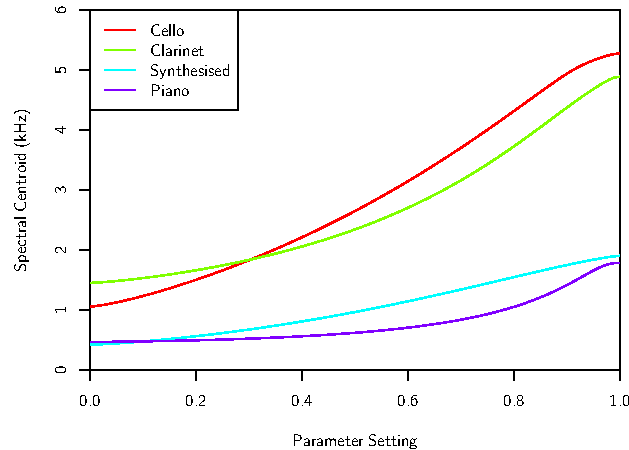
\includegraphics{chapter6/Images/MoveCentroids.pdf}
				\caption{Manipulating the spectral centroids of the test signals.}
				\label{fig:MoveCentroids}
			\end{figure}

			When $P$ is set to zero the input signal is effectively processed by only a low pass filter,
			reducing its spectral centroid. As $P$ is increased more energy is introduced in the higher
			harmonics until the maximum spectral centroid is reached at $P = 1$. For each signal the range of
			values the spectral centroid can take covers approximately two octaves. The spectral structure of
			the two bands determines how the spectral centroid changes within this range.

		\subsubsection*{Parameterisation of The Higher Order Spectral Moments}
			Higher order spectral moments are more difficult to parameterise. The measures depend on the
			displacement of each spectral component from the centroid, skewness and kurtosis measurements also
			depend on the spectral spread. To simplify the control of these moments it is necessary to use
			manipulations which do not alter the moments they depend on. 
			
			Controlling the spread while keeping the centroid constant involves adding or removing energy
			symmetrically about the centroid. Deciding where to add or remove this energy is a complicated
			process. The frequencies of the spectral components are not likely to be symmetrical about the
			centroid meaning different gains must be applied to components either side of the centroid.
			Calculating these gains must be done on a signal by signal basis making if difficult to provide a
			general solution. These problems are compounded further when trying to control the higher order
			moments as the spectral spread must be kept constant as well.

			Intuition about what the spectral moments describe can be used to influence them in a simpler
			manner. These methods do not provide precise control over a specific moment but allow it to be
			increased or decreased.  Furthermore, they will have an effect on all the spectral moments rather
			than one in isolation. 
			
			Spectral spread can be increased by adding energy at frequencies which are more that one spectral
			spread from the centroid or reducing the energy at frequencies within one spectral spread of the
			centroid.  Applying the opposite operations will decrease the spectral spread. This can be
			implemented using a system similar to that in Figure \ref{fig:TwoBandSpectralCentroidSystem}. A
			band of harmonic energy is generated by processing the isolated $f_{0}$ with a nonlinear device
			followed by a band pass filter. This new band can then be summed with the original signal at the
			desired gain. Figure \ref{fig:MoveSpreads} shows the change in spectral spread when the gain, $m$,
			of a spectral band, containing energy between $0.8\mu_{s}$ and $1.2\mu_{s}$, is changed.

			\begin{figure}[h!]
				\centering
				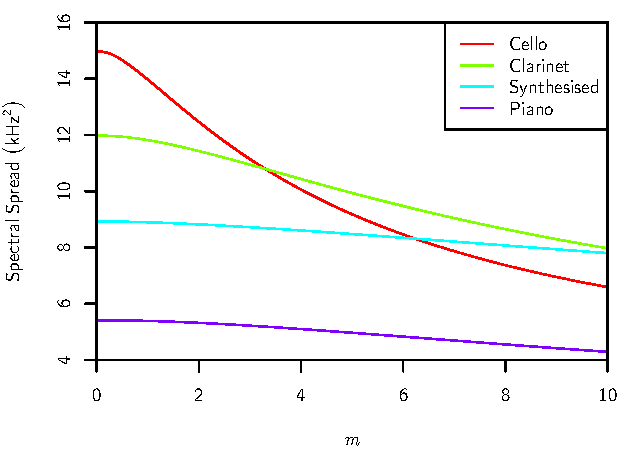
\includegraphics{chapter6/Images/MoveSpreads.pdf}
				\caption{Manipulating the spectral spreads of the test signals.}
				\label{fig:MoveSpreads}
			\end{figure}

			This is a manipulation in which an excitation system has an advantage over linear filtering. The
			ability to generate new bands of energy means that energy can be added near to the spectral
			centroid regardless of whether there was energy there in the input signal.

			Spectral skewness can be increased by applying a spectral tilt about the spectral centroid. A tilt
			with a positive gradient will decrease the skewness, whereas a negative gradient will increase the
			skewness. While the simplest system to achieve this would be a linear filter, an excitation based
			approach can provide a more flexible system in terms of manipulation or preservation of other
			features. Using the system shown in Figure \ref{fig:SuperpositionSystem} a spectral tilt of $k$ dB
			per octave can be applied to the first nine harmonics. This is done by multiplying each harmonic's
			amplitude by $10^{\frac{k}{20}\log_{2} \left( \frac{\nu_{n}}{\mu_{s}} \right)}$. Increasing the
			value of $k$ increases the gradient of the tilt applied and thereby lowers the signal's spectral
			skewness. Figure \ref{fig:MoveSkewnesses} shows the effects of changing $k$ when processing the
			test signals.

			\begin{figure}[h!]
				\centering
				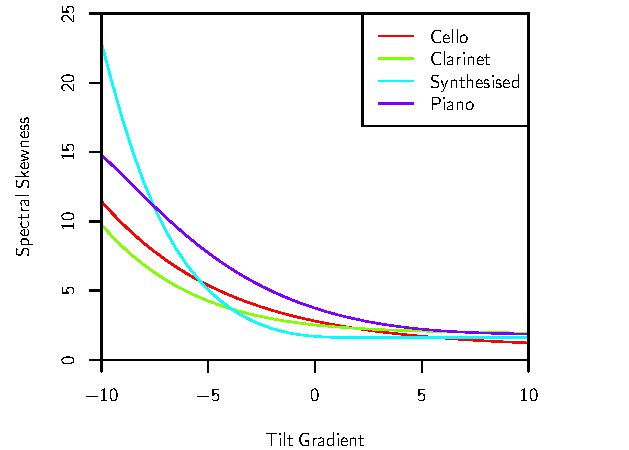
\includegraphics{chapter6/Images/MoveSkewnesses.pdf}
				\caption{Manipulating the spectral skewnesses of the test signals.}
				\label{fig:MoveSkewnesses}
			\end{figure}

			Only controlling the amplitudes of the first nine harmonics imposes restrictions on how the
			spectral skewness can be manipulated. The great amount of control over the low end of the signal's
			spectrum allows for skewness to be easily increased, as evidenced by Figure
			\ref{fig:MoveSkewnesses}.  Decreasing the skewness however, is more difficult. The excitation
			system does not provide such fine control over the high end of a signal's spectrum. Using the
			spectral tilt method with a high positive value for $k$ will greatly attenuate the low order
			harmonics but leave the high order harmonics unprocessed. This means the output skewness will be
			equal to the skewness of the high order harmonics of the signal. This is seen in Figure
			\ref{fig:MoveSkewnesses} where the skewness values all approach some minimum value. Introducing
			more high frequency energy using a nonlinear device, as done when controlling the spectral
			centroid, is a possible solution to this.

			Spectral kurtosis can be changed using the same method as for spectral spread. Increasing the
			energy near the centroid reduces the kurtosis, while removing energy near the centroid increases
			the kurtosis. Figure \ref{fig:MoveKurtoses} shows the effect on the spectral kurtosis of the test
			signal when undergoing the same processing as described for Figure \ref{fig:MoveSpreads}.
			
			\begin{figure}[h!]
				\centering
				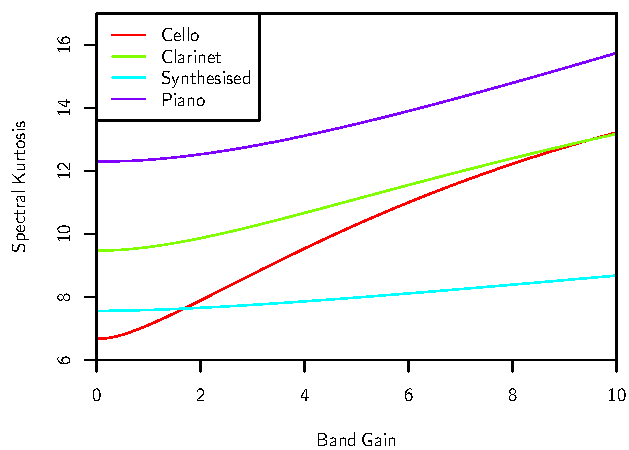
\includegraphics{chapter6/Images/MoveKurtoses.pdf}
				\caption{Manipulating the spectral kurtoses of the test signals.}
				\label{fig:MoveKurtoses}
			\end{figure}

	\subsection{Spectral Irregularity}
	\label{sec:FeatureControl-Parameterisation-Irregularity}
		\citet{beauchamp2007analysis} proposes methods for manipulating the spectral irregularity in additive
		synthesis systems. In effect these involve filtering of the frequency domain representation of a signal,
		applying a filter to the amplitudes of the signal's spectral components. This does not allow the
		irregularity to be set to a precise value but gives control over the direction in which the irregularity
		will change. Low pass filtering of the spectral components' amplitudes will decrease the irregularity while
		a high pass filter will do the opposite.
		
		Both the Krimphoff and Beauchamp irregularities (Equations \ref{eq:KrimphoffIrregularity} and
		\ref{eq:BeauchampIrregularity}) are based on taking the differences between each partial's amplitude and
		the mean amplitude of itself and the two partials surrounding it. Intuitively this value can be increased
		or reduced by moving the amplitudes of the partials away or towards their mean. To implement this using the
		system shown in Figure \ref{fig:SuperpostionSystem} the new amplitudes of the first nine harmonics can be
		calculated using Equation \ref{eq:PartialSmoothing}

		\begin{equation}
			a'_{n} = a_{n} \left( \frac{\sum_{k = 1}^{9} a_{k}}{9a_{n}} \right) ^{P}
			\label{eq:PartialSmoothing}
		\end{equation}

		Where $a'_{n}$ is the new amplitude of the $n$\super{th} partial, $a_{n}$ is the amplitude of the
		$n$\super{th} partial in the input signal, and $P$ is a parameter controlling how the irregularity is
		affected. Negative values of $P$ will increase the irregularity, while small positive values of $P$ will
		decrease the irregularity. The minimum possible irregularity is achieved when $P \approx 1$, higher values
		of $P$ will increase the irregularity again. Figure \ref{fig:MoveIrregularities} shows how each of the
		spectral irregularity measures are affected by changes in the value of $P$.

		\begin{figure}[h!]
			\centering
			\captionsetup[subfigure]{oneside,margin={1cm, 0cm}}
			\subfloat[Krimphoff Irregularity]
			{
				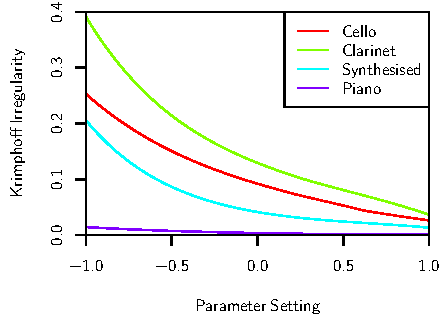
\includegraphics{chapter6/Images/MoveIrregularitiesK.pdf}
				\label{fig:MoveIrregularitiesK}
			}
			\quad
			\subfloat[Jensen Irregularity]
			{
				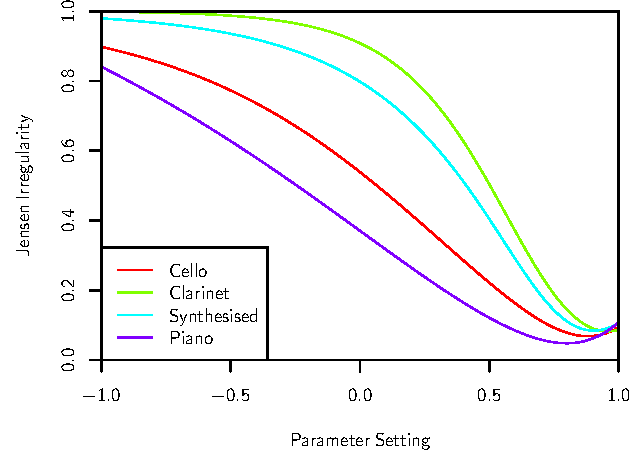
\includegraphics{chapter6/Images/MoveIrregularitiesJ.pdf}
				\label{fig:MoveIrregularitiesJ}
			}
			
			\subfloat[Beauchamp Irregularity]
			{
				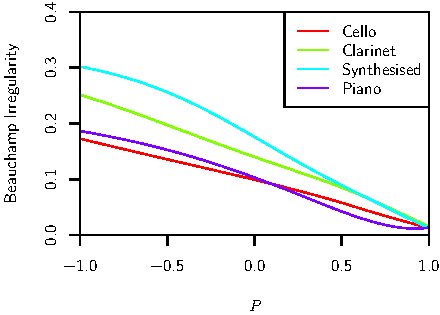
\includegraphics{chapter6/Images/MoveIrregularitiesB.pdf}
				\label{fig:MoveIrregularitiesB}
			}
			\caption{Manipulating the spectral irregularities of the test signals.}
			\label{fig:MoveIrregularities}
		\end{figure}

		As is most notable in Figure \ref{fig:MoveIrregularitiesJ} the value of $P$ which will give the minimum
		flatness depends on the input signal. This is because only the first nine harmonics of each signal are
		being manipulated. The existing irregularity in the higher order harmonics may mean that adjusting the
		first nine harmonics to have the same level, as happens when $P = 1$, will not produce the minimum
		irregularity. The unbounded nature of the Krimphoff irregularity is also visible in Figure
		\ref{fig:MoveIrregularities}.  While the Jensen and Beauchamp irregularities both asymptotically approach a
		maximum as $P$ is reduced the Krimphoff irregularity increases exponentially.

		Achieving this using excitation requires an analysis / resynthesis approach, replacing the existing
		spectral components with excited ones and changing the amplitudes to give the desired irregularity. If the
		analysis stage is removed the complexity of the system can be greatly reduced. The amplitudes of the newly
		excited spectral components can be predetermined and the irregularity manipulated as per Equation
		\ref{eq:PartialSmoothing}. A different number of spectral components can be replaced with excited ones
		depending on how large a timbral variation is desired. Replacing only a few spectral components will
		provide a small amount of control over irregularity while preserving most of the spectrum of the input
		signal. Replacing more spectral components provides more control over the overall irregularity at the cost
		of losing more spectral information from the original.

		An alternate way to influence the irregularity of a signal is through control of the oddness and evenness
		as discussed in Section \ref{sec:FeatureControl-Parameterisation-HarmonicParityRatio}. A signal with a high
		oddness and low evenness (or vice versa) will have a high a spectral irregularity whereas a signal with a
		more even distribution of energy between odd and even harmonics will have a lower irregularity. This allows
		the irregularity of a signal which contains both parities of harmonics can be changed by altering the
		signals oddness or evenness.

	\subsection{Spectral Flatness}
	\label{sec:FeatureControl-Parameterisation-Flatness}
		Spectral flatness is related to spectral irregularity. Many of the techniques to reduce the irregularity
		will also increase the flatness. More precisely, any manipulation which moves the amplitudes of all
		spectral components closer to each other will increase the spectral flatness. To take an example from
		Section \ref{sec:FeatureControl-Parameterisation-Irregularity}, using a low pass filter on the amplitudes
		of the spectral components will increase the flatness of the spectrum.

		As the measure of spectral flatness (Equation \ref{eq:Flatness}) is the ratio of the geometric and
		arithmetic means of the power spectrum, a greater degree of control can be achieved over it by altering one
		of the means while the other remains constant. The method discussed here changes the arithmetic mean while
		preserving the geometric mean. Consider two disjoint sets, $L$ and $H$, which are each composed of the
		indices of $k$ spectral components of the signal, such that the total energy in the spectral components
		denoted by $L$ is less than that of the spectral components denoted by $H$. A gain $m$ is applied to the
		spectral components denoted by set $H$ and the reciprocal gain $\frac{1}{m}$ applied to the spectral
		components denoted by set $L$. The resulting spectral flatness is calculated using Equation
		\ref{eq:FlatnessManipulation}.

		\begin{gather}
			P = \left\{ n | n \in \textbf{N} \land n \leq N \right\} \nonumber \\
			E = P \setminus (L \medcup H) \nonumber \\
			A_{L} = \sum_{n \in L} a_{n}^{2} \quad A_{H} = \sum_{n \in H} a_{n}^{2}
			   \quad A_{E} = \sum_{n \in E} a_{n}^{2} \nonumber \\
			\mathrm{SF} = \frac{N\sqrt[N]{\prod_{n \in P} a_{n}^{2}}}
					   {\frac{A_{L}}{m^{2}} + m^{2}A_{H} + A_{E}}
			\label{eq:FlatnessManipulation}
		\end{gather}

		The spectral flatness can be increased by using a value of $m$ such that $\sqrt{\frac{A_{L}}{A_{H}}} < m <
		1$. The maximum possible flatness which can be achieved with the selected spectral components occurs when
		$m = \sqrt[4]{\frac{A_{L}}{A_{H}}}$. To decrease the spectral flatness a value of $m$ satisfying $0 < m <
		\sqrt{\frac{A_{L}}{A_{H}}}$ or $m > 1$ should be used. When $m = \sqrt{\frac{A_{L}}{A_{H}}}$ the arithmetic
		mean is unchanged, this provides a point at which the energy has been redistributed in the spectrum but the
		spectral flatness remains the same. 

		The gain value, $m$, can be calculated from a simplified control parameter, $P$, using Equation
		\ref{eq:FlatnessControlParameter}. When $P$ is equal to 0 or 1 the spectral flatness will be unchanged.
		Values of $P$ between 0 and 1 will increase the spectral flatness, with the maximum flatness being achieved
		at $P = 0.5$. Finally, when $P > 1$ the spectral flatness will decrease.  Figure \ref{fig:MoveFlatnesses}
		shows the effects of altering this parameter on the spectral flatness of the test signals when both sets,
		$L$ and $H$, are comprised of the indices of three spectral partials.

		\begin{equation}
			m = \sqrt{ \left( \frac{A_L}{A_H} \right) ^{1 - P}}
			\label{eq:FlatnessControlParameter}
		\end{equation}

		\begin{figure}[h!]
			\centering
			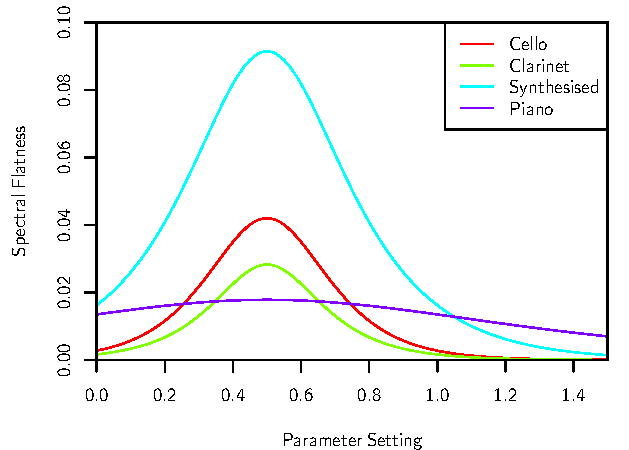
\includegraphics{chapter6/Images/MoveFlatnesses.pdf}
			\caption{Manipulating the spectral flatnesses of the test signals.}
			\label{fig:MoveFlatnesses}
		\end{figure}

		The maximum flatness which can be achieved depends on the flatnesses of the two sets $L$ and $H$.  If these
		sets are themselves flat (i.e. all partials in them have similar amplitudes) the maximum possible flatness
		will be large. If the amplitudes of partials within each set have high variance the capacity for increasing
		the overall flatness is reduced.

		Equation \ref{eq:FlatnessManipulation} provides control over the spectral flatness in a signal where the
		amplitudes of the spectral components are known. As with control of spectral irregularity, an analysis /
		resynthesis technique could be utilised to implement this using harmonic excitation.  Again it is desirable
		to remove the analysis step in order to reduce the complexity of the system.  This can be done by replacing
		a band of spectral components with excited ones. Once a band has been replaced with excited components, the
		levels of these components can then be manipulated to change the flatness of the entire signal. Altering
		the flatness of the excited band using the method in Equation \ref{eq:FlatnessManipulation} allows the
		overall flatness of the output to be influenced. Reducing the arithmetic mean of the power spectrum of the
		excited band also reduces the arithmetic mean of the power spectrum of the output signal. Thus, increasing
		the flatness of the excited band will also increase the flatness of the output signal and decreasing the
		flatness of the band decreases the flatness of the output signal.

		As the spectral flatness measure doesn't depend on the frequencies of the spectral components, deciding
		what two groups of components to apply reciprocal gains to will depend on the desired effect on other
		spectral features. For instance, to have a maximal effect on the odd to even harmonic ratio one could
		select two groups which consist of odd and even harmonics respectively. To have a minimal effect on this
		feature the two groups can both consist of one parity of harmonic.

	\subsection{Spectral Slope}
	\label{sec:FeatureControl-Parameterisation-Slope}
		As discussed in Section \ref{sec:ExcitationEvaluation-Comparison-SpectralCharacteristics} the spectral
		slope of the band of distortion components generated using a static nonlinearity depends on the continuity
		of the nonlinearity's characteristic curve and its derivatives. Using a simple system, similar to that in
		Figure \ref{fig:F0Tracking}, the characteristic curve of the nonlinearity can be changed to influence the
		spectral slope of the output signal. While this 

		The system shown in Figure \ref{fig:SuperpositionSystem} provides more control, allowing for slopes other
		than multiples of 6dB per octave. As with the discussions on spectral irregularity and flatness, an
		analysis / resynthesis approach provides finer control.  To increase the spectral slope by $k$ dB per Hz,
		each spectral component in the signal should have its amplitude, $a_{n}$, multiplied by the value
		$10^{\frac{k}{20}(\nu_{n} - \nu_{1})}$. Figure \ref{fig:MoveSlopes} shows the manipulation of the spectral
		slopes of the test signals.

		\begin{figure}[h!]
			\centering
			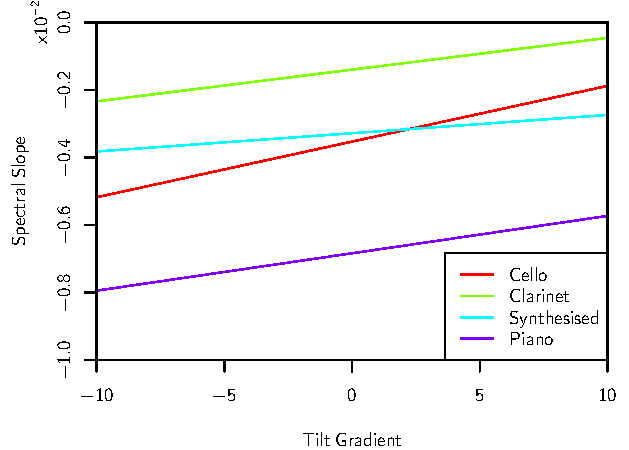
\includegraphics{chapter6/Images/MoveSlopes.pdf}
			\caption{Manipulating the spectral slopes of the test signals.}
			\label{fig:MoveSlopes}
		\end{figure}

		Ideally each line in Figure \ref{fig:MoveSlopes} would have the same gradient, as the signals' spectral
		slopes are being increased by the same factor. They do not however, as only the fist nine harmonics are
		being individually manipulated. The differences, in amplitudes of the higher order harmonics, between the
		signals account for the differences in control of the spectral slope.

		If measuring spectral slope in dB per octave, to increase the slope by $k$dB per octave, each spectral
		component in the signal should have its amplitude, $a_{n}$, multiplied by the value
		$10^{\frac{k}{20}\log_{2} \left( \frac{\nu_{n}}{\nu_{1}} \right)}$.

		If the analysis section is removed the excited spectral components can have their amplitudes set to give
		the desired slope. This is achievable for the lower order harmonics which are generated individually.  The
		static nonlinearity used to generate the higher order harmonics should be chosen to produce a band with a
		roll off as close to that of the desired slope. Generating the high order harmonics in this manner reduces
		complexity at the cost of precise control of the spectral slope.

	\subsection{Tristimulus}
	\label{sec:FeatureControl-Parameterisation-Tristimulus}
		A generalised form of the tristimulus metrics measures the amplitude ratio, $R$, of a specific set of
		spectral components, $S$, and a set which includes that set, $F$. This is shown in Equation
		\ref{eq:GeneralTristimulus}.

		\begin{gather}
			A = \sum_{n \in F} a_{n} \nonumber \\
			B = \sum_{n \in S} a_{n}, \quad S \subseteq F \nonumber \\
			R = \frac{B}{A}
			\label{eq:GeneralTristimulus}
		\end{gather}

		This ration can be adjusted by applying gain to the spectral components in $S$. To attain a particular
		value of $R$ the required gain, $m$, can be calculated using Equation
		\ref{eq:GeneralTristimulusManipulation}.

		\begin{equation}
			m = \frac{R(B - A)}{B(R - 1)}, \quad 0 \leq R < 1
			\label{eq:GeneralTristimulusManipulation}
		\end{equation}

		Similar to the method discussed for controlling spectral centroid, control of tristimulus metrics involves
		altering the energy in specific bands. A reduced version of the system shown in Figure
		\ref{fig:SuperpositionSystem} can be used to control this. The system need only have individual control
		over the levels of the first four harmonics so the exciters for the fifth through ninth harmonics can be
		removed.

		The first tristimulus measure is easily controlled through applying gain to the isolated $f_{0}$.  The
		other two measures can be controlled in different ways depending on the requirements of the system.
		Individually controlling the levels of the second through fourth harmonics allows the second tristimulus
		measure to be manipulated while a more general nonlinear device can be used to generate higher order
		harmonics. As with the spectral centroid, using excitation to achieve this provides more flexibility as the
		tristimulus can be changed while preserving other features. For example, if the odd to even harmonic ratio
		needs to remain the same, but the second tristimulus change, different amounts of excitation can be applied
		to the second through fourth harmonics.

		Figure \ref{fig:MoveTristimulus1} shows how the first tristimuli of the test signals change when the gain
		is applied at their $f_{0}$ using the system shown in Figure \ref{fig:SuperpositionSystem}.

		\begin{figure}[h!]
			\centering
			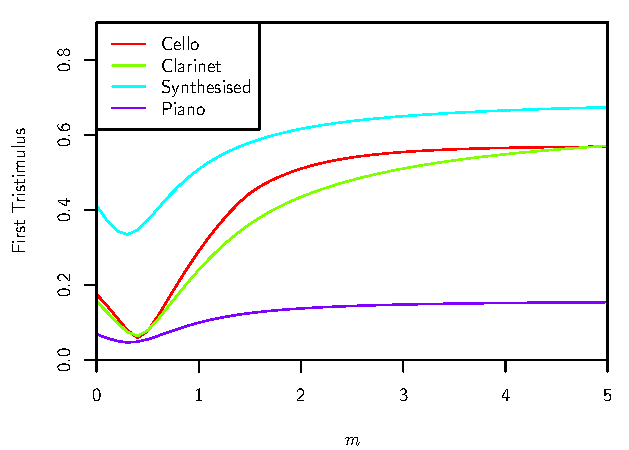
\includegraphics{chapter6/Images/MoveTristimulus1.pdf}
			\caption{Manipulating the first tristimuli of the test signals.}
			\label{fig:MoveTristimulus1}
		\end{figure}

		The maximum achievable first tristimulus value is determined by both the content of the input signal and
		the order of the filters used in the implementation of the excitation system. The system used for the
		values shown in Figure \ref{fig:MoveTristimulus1} used second order IIR filters. This means that the
		isolated $f_{0}$ signal contains energy in some of the higher order spectral partials. In sounds where the
		$f_{0}$ has significantly less amplitude than subsequent spectral partials this is particularly
		problematic. The piano signal used for testing illustrates this. In this case the isolated $f_{0}$ signal
		has more energy in the second harmonic than at the $f_{0}$, severely reducing the maximum value which the
		first tristimulus can be altered to.  Using higher order filters will alleviate this problem at the cost of
		increased processing complexity.

		The order of the filters is also responsible for the initial decrease in tristimulus value with increasing
		gain. The $f_{0}$ is removed from the original signal using a high pass filter. The lower order this filter
		the more of a remnant of the $f_{0}$ remains. This initial decrease in the first tristimulus is due to
		destructive superposition between the isolated $f_{0}$ and this remnant. Again, increasing the order of the
		filters used in the system will reduce these effects.

		Control of the second tristimulus can be achieved with the same system, this time applying gain at to the
		second third and fourth excited harmonics. Figure \ref{fig:MoveTristimulus2} how the tristimulus value
		changes with increasing gain.

		\begin{figure}[h!]
			\centering
			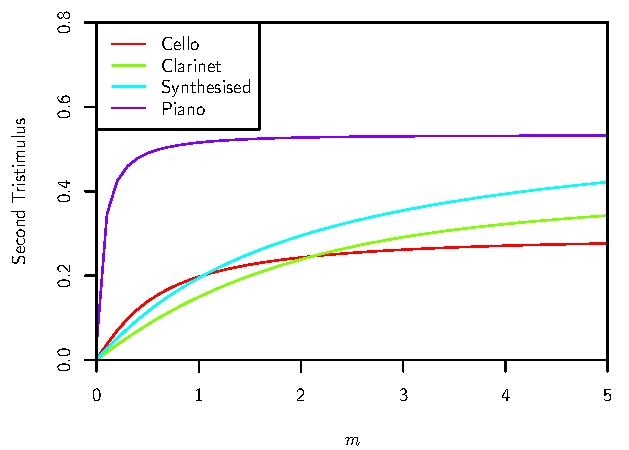
\includegraphics{chapter6/Images/MoveTristimulus2.pdf}
			\caption{Manipulating the second tristimuli of the test signals.}
			\label{fig:MoveTristimulus2}
		\end{figure}

		As with control of the first tristimulus, the order of the filters used determines the maximum value the
		second tristimulus will take. The relationship is a more complex one however, as there is a nonlinear
		element to the system. The isolated $f_{0}$ signal will contain some energy at higher order partials.  When
		this signal is used to generate new harmonics some of the intermodulation components will be higher in
		frequency than the desired harmonic. This results in more energy being introduced above the fourth
		harmonic, reducing the maximum possible second tristimulus.

		The third tristimulus is more easily controlled using the same system as used for controlling the spectral
		centroid (Figure \ref{fig:TwoBandSpectralCentroidSystem}). A band of high order harmonics is generated from
		the isolated $f_{0}$ using a static nonlinearity and a high pass filter.  Figure \ref{fig:MoveTristimulus3}
		shows how changing the gain of this band effects the third tristimulus of the test signals.

		\begin{figure}[h!]
			\centering
			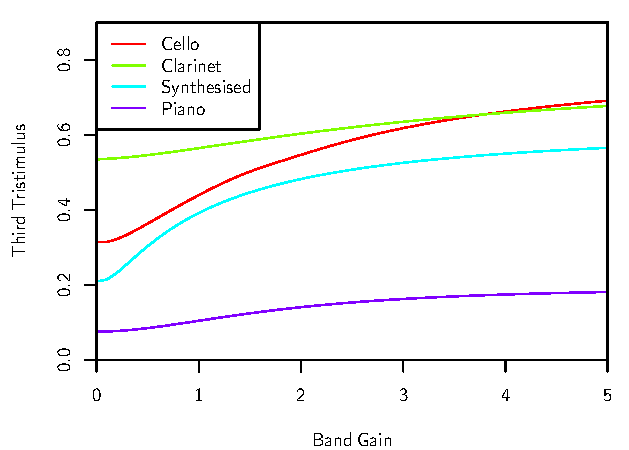
\includegraphics{chapter6/Images/MoveTristimulus3.pdf}
			\caption{Manipulating the third tristimuli of the test signals.}
			\label{fig:MoveTristimulus3}
		\end{figure}

		Again, second order IIR filters have been used to filter out the lower order harmonics from the excited
		signal.	These low order filters do not remove all the energy in the first 4 harmonics thereby limiting how
		high the third tristimulus can be made.

	\subsection{Odd to Even Harmonic Ratio}
	\label{sec:FeatureControl-Parameterisation-HarmonicParityRatio}
		The odd to even harmonic ratio, Equation \ref{eq:HarmonicParityRatio}, can easily be altered by applying
		gain to the odd harmonics. The required gain factor, $m$, is calculated using Equation
		\ref{eq:HarmonicParityRatioManipulation}.

		\begin{equation}
			m = \sqrt{\frac{\mathrm{OER}\sum_{1 \leq n \leq N, n \text{ is even}} h_{n}^{2}}
				       {\sum_{1 \leq n \leq N, n \text{ is odd}} h_{n}^{2}}},
				       \quad \mathrm{OER} \geq 0;
		       \label{eq:HarmonicParityRatioManipulation}
		\end{equation}

		The oddness and evenness, Equations \ref{eq:Oddness} and \ref{eq:Evenness}, can be generalised to give
		Equation \ref{eq:GeneralOddness}.

		\begin{gather}
			A = \sum_{n \in F} a_{n}^{2} \nonumber \\
			B = \sum_{n \in S} a_{n}^{2}, \quad S \subseteq F \nonumber \\
			R = \sqrt{\frac{B}{A}}
			\label{eq:GeneralOddness}
		\end{gather}

		Like Equation \ref{eq:GeneralTristimulus} this measures the ratio of amplitudes of a set of frequencies and
		a larger set of frequencies. This time using the squares of the amplitudes and taking the square root
		afterwards. The value of the ratio can be altered by applying gain to the spectral components in the set
		$S$. The required gain factor, $m$, is calculated using Equation \ref{eq:GeneralOddnessManipulation}.

		\begin{equation}
			m = \sqrt{\frac{R^{2}(B - A)}{B(R^{2} - 1)}}, \quad 0 \leq R < 1
			\label{eq:GeneralOddnessManipulation}
		\end{equation}

		For control over the oddness or evenness of a signal, a system which provides control over individual
		harmonics is not necessary. While this level of control allows for more complex manipulations a simpler
		system can be employed if only the oddness and evenness are to be changed.  Such a system is shown in
		Figure \ref{fig:HarmonicParitySystem}.

		\begin{figure}[h!]
			\centering
			\begin{tikzpicture}
				\node (In) at (-1, -2.25) {$x[n]$};
				\coordinate (InMid) at (0, -2.25);
				\draw (In) -- (InMid);

				\coordinate (Side) at (0, -1.25);
				\draw (InMid) -- (Side);

				\node (F0) [draw] at (2, -1.25) {$f_{0}$ Tracker};
				\node (F0Filter) [draw] at (2, -2.25) {LPF};
				\draw (InMid) -- (F0Filter);
				\draw (F0) -- (F0Filter);
				\draw (Side) -- (F0);

				\node (Add) [operator] at (11.5, -2.25) {+};

				\coordinate (ExciterIn) at (4, -2.25);
				\draw (F0Filter) -- (ExciterIn);

				% odd harmonics
				\coordinate (OddIn) at (4, -1.25);
				\node (Odd) [draw] at (6, -1.25) {Odd Harmonics};
				\draw (OddIn) -- (Odd);

				\node (OddFilter) [draw] at (8.5, -1.25) {Filter};
				\draw (Odd) -- (OddFilter);

				\node (OddGain) [gain] at (10, -1.25) {};
				\draw (OddFilter) -- (OddGain);
				\coordinate (OddOut) at (10.5, -1.25);
				\draw (OddGain) -- (OddOut);
				\draw (OddOut) -- (Add);

				% even harmonics
				\coordinate (EvenIn) at (4, -2.25);
				\draw (OddIn) -- (EvenIn);
				\node (Even) [draw] at (6, -2.25) {Even Harmonics};
				\draw (EvenIn) -- (Even);

				\node (EvenFilter) [draw] at (8.5, -2.25) {Filter};
				\draw (Even) -- (EvenFilter);

				\node (EvenGain) [gain] at (10, -2.25) {};
				\draw (EvenFilter) -- (EvenGain);
				\coordinate (EvenOut) at (10.5, -2.25);
				\draw (EvenGain) -- (EvenOut);
				\draw (EvenOut) -- (Add);

				% through
				\coordinate (Through) at (0, -3.25);
				\draw (InMid) -- (Through);
				\node (ThroughFilter) [draw] at (8.5, -3.25) {Filter};
				\draw (Through) -- (ThroughFilter);
				\node (ThroughGain) [gain] at (10, -3.25) {};
				\draw (ThroughFilter) -- (ThroughGain);
				\coordinate (ThroughOut) at (10.5, -3.25);
				\draw (ThroughGain) -- (ThroughOut);
				\draw (ThroughOut) -- (Add);

				\node (Out) at (12.75, -2.25) {$y[n]$};
				\draw (Add) -- (Out);
			\end{tikzpicture}
			\caption{A system to control the levels of odd and even order harmonics individually.}
			\label{fig:HarmonicParitySystem}
		\end{figure}

		This system uses two parallel static nonlinearities to generate two signals consisting of only odd
		harmonics and even harmonics respectively. The properties of these nonlinearities can be adjusted to shape
		the spectra of each of these signals which are further shaped through linear filtering.  The gains of these
		two signals allow control over the oddness and evenness of the signal using Equation
		\ref{eq:GeneralOddnessManipulation}.

		The odd and even harmonics in a signal could be separated using linear filters. This approach requires in
		depth analysis of the signal adding complexity and possible delay to the system but has some advantage in
		preservation of signal characteristics. When using excitation this complexity is reduced but the problems
		discussed in Section \ref{sec:FeatureControl-Systems-Superposition} become apparent. To elicit full control
		over the levels of the odd and even harmonics using the system shown in Figure
		\ref{fig:HarmonicParitySystem} all the harmonic content in the output signal is generated by the
		nonlinearities. This is likely to cause a dramatic change in timbre as most of the information present in
		the original signal has been replaced. 

		A method to counteract this is to only excite even or odd harmonics in the signal at any one time.  The
		relative levels of odd and even harmonics can still be adjusted but some more of the original signals
		spectral shape is preserved. Avoiding superposition still remains difficult in this situation as it would
		mean filtering out alternate harmonics in the input signal. Allowing superposition to occur sacrifices
		precise control in order to maintain some of the input's characteristics.

		An example of how the system in Figure \ref{fig:HarmonicParitySystem} can be used is as follows.  The
		isolated $f_{0}$ of each test signal id processed with both even and odd hard clipping functions to
		generate separate bands of each parity of harmonic. Each band of harmonics is then low passed filtered with
		a cutoff at the frequency of the ninth harmonic and the original signal is high pass filtered at the same
		frequency. The ninth harmonic is chosen due to it being the highest individually resolved harmonic as
		discussed in Section \ref{sec:FeatureControl-Systems-SpectralShaping}. The three signals are then summed at
		different ratios to control the evenness or oddness of the output. Figure \ref{fig:MoveParities} shows the
		effects of manipulating the levels of odd and even order harmonics in this way. The original signal remains
		at unity gain whereas the gains of the harmonic bands are determined by a parameter, $P$.  Odd order
		harmonics are multiplied by a gain of $P$ and even order harmonics by $1 - P$.

		\begin{figure}[h!]
			\centering
			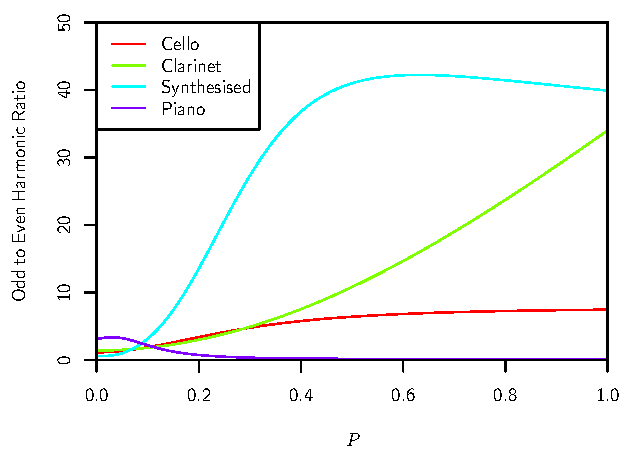
\includegraphics{chapter6/Images/MoveParities.pdf}
			\caption{Manipulating the odd to even harmonic ratios of the test signals.}
			\label{fig:MoveParities}
		\end{figure}

		Here we see how the spectral content of the input signal influences the effects of the processing.  The
		$\mathrm{OER}$ of the clarinet signal seems to be the easiest to control. This can be attributed to the
		high oddness of the unprocessed clarinet signal, the $f_{0}$ is easier to isolate because there is very
		little energy in the second harmonic. With a better isolated $f_{0}$ the two bands of excited harmonics
		will be better separated with respect to the parities of harmonics they contain.

		The cello and synthesised signals both exhibit a limit on how high the $\mathrm{OER}$ can be made. This
		is due to both bands of excited harmonics containing both parities of harmonic.  The general upward trend
		for both signals illustrates that the two bands generated do contain the majority of their energy in the
		correct parity harmonics but higher order filtering of the $f_{0}$ is needed to better segregate them. The
		decrease in $\mathrm{OER}$ seen for the synthesised signal is due to destructive superposition between
		the harmonics in the three signals being summed.

		The system discussed here provides no control over the $\mathrm{OER}$ of the piano signal. This is again
		due to the low amplitude $f_{0}$. The isolated $f_{0}$ signal contains the majority of its energy in the
		second harmonic. This causes the two bands of generated harmonics to both contain mostly even order
		harmonics, meaning the resulting signal will have a high evenness, or low $\mathrm{OER}$.

	\subsection{Inharmonicity}
	\label{sec:FeatureControl-Parameterisation-Inharmonicity}
		While it is reasonably simple to introduce inharmonicity in harmonic excitation systems, controlling the
		inharmonicity of a signal is a more complicated problem. The system shown in Figure
		\ref{fig:InharmonicitySystem} can be use to apply multiple approaches approach to this problem. 

		A simple two band system leaves the lower partials of the system unaltered and generates a high band using
		a static nonlinearity and filtering. The inharmonicities in this high band will be amplified versions of
		those in the original signal. This approach is not applicable in a number of situations such as when the
		input only contains perfectly harmonic partials or when the desired result is a signal with reduced
		inharmonicity.
		
		The inverse system, in which the high frequencies are left unaltered and the low frequency partials are
		generated individually, provides a greater amount of control over the inharmonicity of the resulting
		signal. The newly generated partials can be put at frequencies closer to harmonics than the originals
		reducing the overall inharmonicity. It also allows for generation of inharmonic partials in a signal with
		zero inharmonicity. 

		This system is more complicated both in computation and use. Because the inharmonicity metric (Equation
		\ref{eq:Inharmonicity}) depends on the frequencies of every partial, there are numerous ways a signal can
		be manipulated resulting in the same value for the inharmonicity. When manipulating the inharmonicity a
		decision needs to be made as to which partials are to be made inharmonic and by how much. One method of
		deciding this is to model it on the vibrational modes of an acoustic instrument, ensuring a natural set of
		inharmonic partials. To increase the inharmonicity the frequencies of the partials can be moved from being
		harmonic towards the frequencies indicated by the model.

		One such model is that given by \citet{rossing2002the} for calculating the frequencies of the spectral
		partials of piano strings. In this model the frequencies of each partial are determined by an inharmonicity
		factor, $A$, using Equation \ref{eq:PianoInharmonicity}. In the modelling of piano timbre the value of $A$
		is calculated from the physical properties of the piano string. For creative purposes the value of $A$ can
		be arbitrarily set.

		\begin{equation}
			a_{n} = nf_{0} \left( 1 + \left( n^{2} - 1 \right) A \right);
			\label{eq:PianoInharmonicity}
		\end{equation}

		Using the system shown in Figure \ref{fig:InharmonicitySystem} the inharmonicities of the first nine
		harmonics of a signal can be set according to this model. Figure \ref{fig:MoveInharmonicities} shows how
		the resulting inharmonicity changes with the inharmonicity factor $A$.

		\begin{figure}[h!]
			\centering
			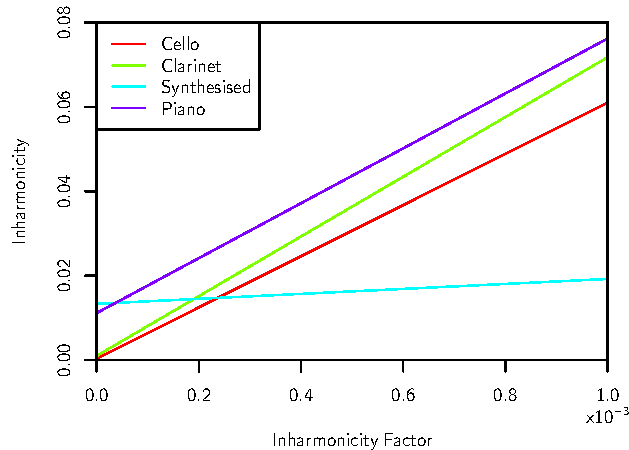
\includegraphics{chapter6/Images/MoveInharmonicities.pdf}
			\caption{Manipulating the inharmonicities of the test signals.}
			\label{fig:MoveInharmonicities}
		\end{figure}

		As only the first nine harmonics are being altered, the degree to which the inharmonicity can be
		manipulated depends on the spectral content of the input signal. In the synthesised signal all of the
		spectral partials are at perfectly harmonic frequencies and there is significant energy in the harmonics
		with higher order than the ninth. The inharmonic signal generated from the synthesised signal then still
		has a significant amount of energy in perfectly harmonic partials giving it a low inharmonicity. This
		reduces the range of values which the resulting inharmonicity can take. The other three signals all have
		higher spectral roll off, such that the influence of their existing high order partials has a smaller
		effect on the overall inharmonicity.

		The issue of higher order harmonics reducing the maximum inharmonicity could be counteracted by adding an
		addition frequency shifter to the system. This shifter would operate on the filtered input signal and shift
		all the higher order partials by the same amount.

%\section{Controlling Features with Exciters}
%\label{sec:FeatureControl-Control}
%	This section will take the systems discussed in Section \ref{sec:FeatureControl-Systems} and use them to alter
%	audio features using the parametrisation techniques given in Section \ref{sec:FeatureControl-Parameterisation}.
%	The system shown in Figure \ref{fig:InharmonicitySystem} provides sufficient flexibility for implementing the
%	majority of these manipulations. The full extent of this system is not needed for some of the simpler modifications
%	so various subsystems of it are used.

\chapter{Validation of Timbral Models}
\label{chap:PerceptualExperiments}

\section{Introduction}
\label{sec:PerceptualExperiments-Introduction}
	The techniques proposed in Chapter~\ref{chap:FeatureControl} provide monotonic control over specific audio
	features, these can be combined with the acoustic correlates discovered in Chapter~\ref{chap:TimbreEvaluation} to
	build intuitive effects which can be used without this specialist knowledge. These timbral control effects can be
	given perceptual control parameters labelled with commonly used semantic descriptors. Novice users can then select
	which effect to use based on the names of its parameters. Additionally, when using the effect, they are able to
	more easily make creative decisions without having to translate them to traditional control parameter settings.

	This chapter presents two experiments that evaluate the performance of timbral control systems proposed in this
	work. The first experiment (Section~\ref{sec:PerceptualExperiments-Reconstruction}) compares the abilities of
	different excitation methods in generating individual harmonics to reconstruct degraded signals. Three different
	systems are used to reconstruct signals which have been degraded by the removal of energy at specific harmonics.
	These reconstructed signals are then evaluated, both objectively and subjectively, in terms of how perceptually
	similar they are to the original, non-degraded signal. The second experiment
	(Section~\ref{sec:PerceptualExperiments-SemanticControl}) uses the results discussed in
	Chapter~\ref{chap:TimbreEvaluation} to inform the design of harmonic excitation effects which provide control over
	a particular perceptual parameter. The performance of these effects is first evaluated objectively, through
	comparison with the timbre spaces constructed in Section~\ref{sec:TimbreEvaluation-Analysis-TimbreSpaces}. Then
	subjective evaluation is carried out by asking listening test participants to describe the timbral manipulations
	applied by the effect and comparing their responses to the descriptor clustering performed in
	Section~\ref{sec:TimbreEvaluation-Analysis-TermClustering}.

\section{Reconstruction of Individual Harmonics}
\label{sec:PerceptualExperiments-Reconstruction}
	As discussed in Chapter~\ref{chap:ExcitationEvaluation}, control over the shape of a signal's spectrum is best
	attained by using systems which allow for manipulation of the levels of individual harmonics in the output. This
	flexibility is not only useful for building creative effects, it can also be used for the reconstruction of
	degraded signals; a process known as audio inpainting \citep{adler2012audio}. These processes use a variety of
	techniques to reintroduce portions of audio which have been lost / degraded by interference or the limitations of
	recording equipment. Individual harmonic generation methods are particularly useful where a harmonically structured
	spectrum needs to be reconstructed, such as when audio has been bandlimited to reduce its storage / transmission
	size.

	Several of the harmonic excitation systems discussed in Section~\ref{sec:FeatureControl-Systems} rely on the
	generation of individual harmonics of the input signal.  Ideally, when a new harmonic is added to a signal using
	one of these systems, it should sound natural: the resulting signal should sound as though it came from a single
	source. A poorly generated harmonic may be perceived as a new sinusoid, completely separate from the original input
	signal as discussed in Section~\ref{sec:FeatureControl-Systems-Individuals}.  Harmonic generation methods can be
	evaluated by how naturally they are able reconstruct signals from which harmonics have been removed. In this
	section an experiment evaluating the performance of three different harmonic generation methods is presented,
	originally presented by \citet{enderby2013methods}.

	\subsection{Harmonic Reconstruction Systems}
	\label{sec:PerceptualExperiments-Reconstruction-Systems}
		Missing harmonics can be reintroduced by generating them from the information remaining in a degraded
		signal. This can be achieved using a spectral shaping system similar to that shown in
		Figure~\ref{fig:SpectralShapingSystem}. Each harmonic, $h_{i}[n]$, is generated individually and then
		summed to create the final output, $y[n]$. Rather than shaping the spectrum to achieve a musical effect,
		the gains for each harmonic are set to reconstruct the shape of the original spectrum. The amplitude ratio
		between the $f_{0}$ and a particular harmonic in a signal may vary with time. This system reconstructs
		harmonics with a constant amplitude ratio to the $f_{0}$, introducing error to the reconstruction.
		Depending on the excitation method used to generate the individual harmonics, further errors will be
		introduced as discussed in Section~\ref{sec:ExcitationEvaluation-Comparison}. For example, the
		\acrshort{ssba} technique is non-homogeneous and the \acrshort{iap} technique does not bound the highest
		order of distortion introduced when the input contains more than one frequency component. In this section
		three methods of generating individual harmonics are assessed to determine the audibility of these errors.

		The first method of reconstructing the harmonics is based on synthesis of new sinusoids and is illustrated
		in Figure~\ref{fig:Synthesise}. First, the \acrshort{stft} of the input signal is calculated. The amplitude
		of the $f_{0}$ in each frame of this \acrshort{stft} is then found and these values interpolated to
		generate an amplitude envelope for the input signal's $f_{0}$. This amplitude envelope is then used in the
		synthesis of a sinusoid at the frequency of the desired harmonic.

		\begin{figure}[h!]
			\centering
			\begin{tikzpicture}
				\node (In) at (-1, 1) {$x[n]$};
				\coordinate (InMid) at (0, 1);
				\draw (In) -- (InMid);

				\coordinate (Side) at (0, 2.5);
				\draw (InMid) -- (Side);

				\node (STFT) [draw] at (1.25, 1) {\acrshort{stft}};
				\draw (InMid) -- (STFT);

				\node (F0) [draw] at (5.63, 2.5) {$f_{0}$ Tracker};
				\draw (Side) -- (F0);

				\coordinate (F0Node) at (5.63, 1.75);
				\draw (F0) -- (F0Node);

				\node (Amp) [draw] at (3.76, 1) {Amplitude Envelope};
				\coordinate (AmpNode) at (3.76, 1.75);
				\draw(F0Node) -- (AmpNode);
				\draw(AmpNode) -- (Amp);
				\draw (STFT) -- (Amp);

				\node (Synth) [draw] at (7.5, 1) {Sine Wave Synthesiser};
				\coordinate (SynthNode) at (7.5, 1.75);
				\draw(F0Node) -- (SynthNode);
				\draw(SynthNode) -- (Synth);
				\draw (Amp) -- (Synth);

				\node (Out) at (10.5, 1) {$h_{i}[n]$};
				\draw (Synth) -- (Out);
			\end{tikzpicture}
			\caption{The system used to generate new harmonics through synthesis.}
			\label{fig:Synthesise}
		\end{figure}

		The other two harmonic generation methods use the system illustrated in Figure~\ref{fig:FilterAndShift},
		isolating the $f_{0}$ with a band pass filter and then using a frequency shifting technique to change the
		frequency to that of the desired harmonic. The two frequency shifting techniques used in this experiment
		are \acrshort{ssba} (Section~\ref{sec:Excitation-Methods-SSBA}) and \acrshort{iap}
		(Section~\ref{sec:Excitation-Methods-IAP}).

		\begin{figure}[h!]
			\centering
			\begin{tikzpicture}
				\node (In) at (0, 1) {$x[n]$};
				\coordinate (InMid) at (1, 1);
				\draw (In) -- (InMid);

				\coordinate (Side) at (1, 2);
				\draw (InMid) -- (Side);

				\node (F0) [draw] at (2.5, 2) {$f_{0}$ Tracker};
				\node (Filter) [draw] at (2.5, 1) {BPF};
				\draw (InMid) -- (Filter);
				\draw (Side) -- (F0);
				\draw (F0) -- (Filter);

				\node (Shifter) [draw] at (5, 1) {Frequency Shifter};
				\draw (Filter) -- (Shifter);

				\node (Out) at (7.35, 1) {$h_{i}[n]$};
				\draw (Shifter) -- (Out);
			\end{tikzpicture}
			\caption{The system used to generate new harmonics using the \acrshort{ssba} and \acrshort{iap}
				 techniques.}
			\label{fig:FilterAndShift}
		\end{figure}

	\subsection{Methodology}
	\label{sec:PerceptualExperiments-Reconstruction-Methodology}
		\subsubsection*{Stimuli Generation}
			The harmonic reconstruction systems were evaluated using the same four audio signals used in
			Section~\ref{sec:FeatureControl-Parameterisation} to assess audio feature parameterisation
			techniques (cello, clarinet, synthesised and piano). For each signal the third through ninth
			harmonics were removed using a 2001\super{st} order \acrshort{fir} band reject filter, with the
			stopband starting at 2.5$f_{0}$ and ending at 9.5$f_{0}$. This was in order to cause significant
			degradation in the quality of the signal, such that the difference is plainly audible to the
			majority of listeners. The second harmonic was left in the signal to pose a challenge to the
			\acrshort{ssba} and \acrshort{iap} methods. As mentioned previously, the performance of these
			methods depends on how well the $f_{0}$ is isolated.  Retaining the second harmonic allows for the
			effect of filter order on the performance of the system to be assessed. Spectrograms of the cello
			signal before and after this process are shown in Figures \ref{fig:CelloSpectrogram} and
			\ref{fig:CelloFilteredSpectrogram}. 

			\begin{figure}[h!]
				\centering
				\captionsetup[subfigure]{oneside,margin={1cm, 0cm}}
				\subfloat[Unprocessed Signal]
				{
					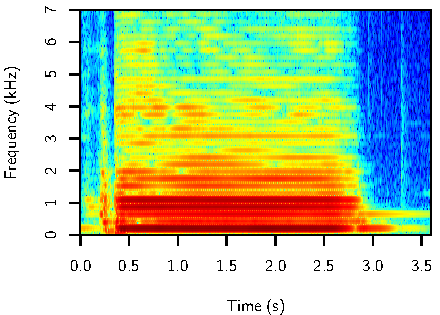
\includegraphics{chapter7/Images/CelloSpectrogram.pdf}
					\label{fig:CelloSpectrogram}
				}
				\quad
				\subfloat[Filtered Signal]
				{
					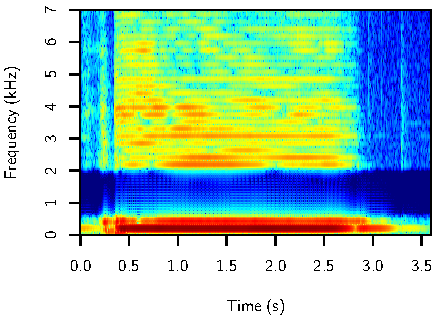
\includegraphics{chapter7/Images/CelloFilteredSpectrogram.pdf}
					\label{fig:CelloFilteredSpectrogram}
				}
				\caption{Spectrograms of the cello signal.}
				\label{fig:CelloSpectrograms}
			\end{figure}

			Test stimuli were created by reintroducing the third through ninth harmonics to the filtered
			signals using the systems described in
			Section~\ref{sec:PerceptualExperiments-Reconstruction-Systems}. In order to reduce the number of
			variables, each of the unprocessed signals was analysed prior to the creation of the test stimuli.
			The $f_{0}$ of each signal was measured along with the mean amplitudes of the third through ninth
			harmonics.  This information was then used in the reconstruction of the signal, mitigating any
			inaccuracies which may be introduced by calculating it in real time and allowing the naturalness of
			the generated harmonics to be assessed more thoroughly.

			Eleven test stimuli were created from each of the original four signals. The first two being the
			unprocessed signal and the filtered signal. The remaining nine were reconstructions of the original
			signal from the filtered signal. Each signal was reconstructed three times with each system, using
			different parameters each time. For the synthesis method the window length of the \acrshort{stft}
			was changed, taking values of 50, 100 and 500 samples. As the window length increases the frequency
			resolution of the spectrum increases, allowing for more accurate calculation of the amplitude of
			the $f_{0}$.  Longer window length however will decrease the temporal resolution of the system,
			smoothing the extracted amplitude envelope. Care must be taken to not increase the \acrshort{stft}
			window length such that this smoothing starts to reduce the accuracy of the extracted amplitude
			envelope.  For the \acrshort{ssba} and \acrshort{iap} methods, a different order \acrshort{fir}
			filter was used to isolate the $f_{0}$. The filters used were windowed sinc filters with orders of
			50, 100 and 500 and using the Blackman window to maximise stopband attenuation
			\citep{schlichtharle2011digital}. As the filter order is increased, the level of the second
			harmonic in the isolated $f_{0}$ decreases.  This leads to a more sinusoidal input to the harmonic
			generation systems, reducing the amount of intermodulation distortion introduced.

			The generation of samples using the synthesis method is not directly comparable to that using the
			\acrshort{ssba} and \acrshort{iap} methods because the \acrshort{stft} window length is not
			comparable with filter order.  The values for these parameters were chosen such that the
			differences between the reconstructions were easily audible. Increasing either of the parameters
			results in a more computationally complex system which should increase the quality of the resulting
			reconstruction.

		\subsubsection*{Objective Evaluation}
			An approximation of the perceptual difference between the stimuli and the relevant audio signal is
			measured using the $R_{\mathrm{nonlin}}$ metric proposed by \citet{tan2004predicting}. As discussed
			in Section~\ref{sec:Excitation-Analysis-Metrics}, this is a metric which uses psychoacoustic models
			of the human hearing system to judge the perceived level of distortion in a signal. It is
			calculated by comparing the degraded signal against the non-degraded signal, returning a value
			between 0 and 1; 1 denoting a signal which is indistinguishable from the original and lower values
			describing signals with a higher level of perceivable distortion.

		\subsubsection*{Subjective Evaluation}
			The performance of the reconstruction systems was evaluated subjectively using series a of multiple
			stimulus listening tests using the \acrshort{mushra} methodology \citep{mushra2014}. Each test is
			split into two phases, a training phase and an evaluation phase. In the training phase,
			participants are presented with an interface (Figure~\ref{fig:MushraTraining}) which allows them to
			audition every one of the stimuli. Participants are asked to listen to each of them in comparison
			with the relevant reference (the unprocessed signal) in order to learn the range of degradation
			present across stimuli. To ensure participants listen to each individual stimulus, the interface
			will not allow them to proceed to the evaluation phase until every stimulus has been played at
			least once.  Buttons for stimuli which have yet to be auditioned appear red in the interface while
			those which have been played will change to green. The button for the currently playing stimulus is
			highlighted in blue.

			\begin{figure}[h!]
				\centering
				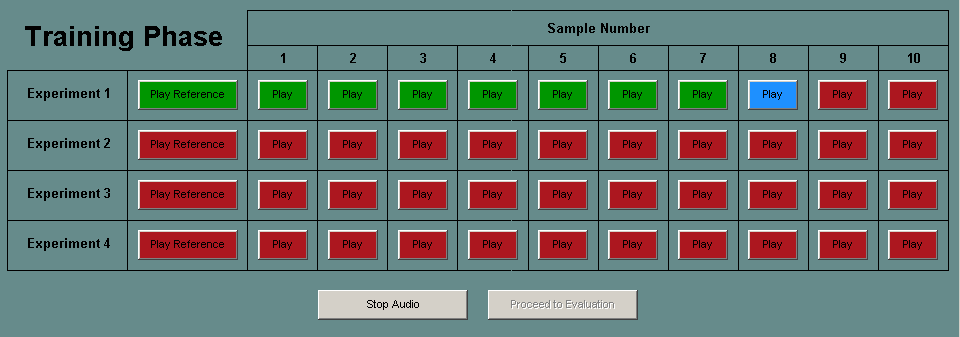
\includegraphics[width=0.95\textwidth]{chapter7/Images/MushraTraining.png}
				\caption{The training phase interface.}
				\label{fig:MushraTraining}
			\end{figure}

			During the evaluation phase, participants are presented with all stimuli created from the same
			signal at once. They were asked to grade how well each of the stimuli recreate the reference
			stimuli (the unprocessed signal) on a scale from 0 to 100. The scale is shown in
			Figure~\ref{fig:MushraScale} and the full interface in Figure~\ref{fig:MushraEvaluation}.

			\begin{figure}[h!]
				\centering
				\begin{tikzpicture}
					\draw(0, 0) -- (7.5, 0);

					\foreach \x/\xvalue in {0/0, 1.5/20, 3/40, 4.5/60, 6/80, 7.5/100}
						\draw (\x, 0pt) -- (\x, 3pt)
						(\x, 0pt) node[below] {\xvalue};

					\foreach \x/\xtext in {0.75/Bad, 2.25/Poor, 3.75/Fair, 5.25/Good, 6.75/Excellent}
						\draw (\x, 3pt) node[above] {\xtext};
				\end{tikzpicture}
				\caption{The grading scale used in the evaluation phase.}
				\label{fig:MushraScale}
			\end{figure}

			Among the stimuli to be graded were a hidden reference and anchor. These are included in order to
			assess the performance of test participants. The hidden reference is a repetition of the reference
			signal and as such should be given a grade of 100 as there is no difference between it and the
			reference. The anchor is the degraded signal and should be graded worse than the all the other
			stimuli as no attempt has been made to reconstruct the its missing harmonics. If a participant does
			not grade the hidden reference and anchor in this way their results may not be reliable and should
			be removed from the dataset.

			\begin{figure}[h!]
				\centering
				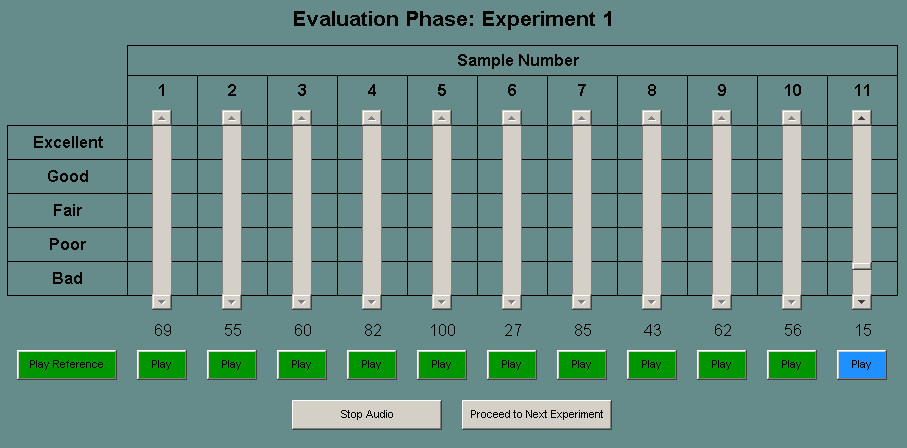
\includegraphics[width=0.95\textwidth]{chapter7/Images/MushraEvaluation.png}
				\caption{The evaluation phase interface.}
				\label{fig:MushraEvaluation}
			\end{figure}

			This evaluation phase is repeated for each of the original audio signals. The order in which the
			evaluation phases for each signal were presented to participants was randomised, along with the
			order in which the stimuli appear in the interface, in order to mitigate any effect the order in
			which stimuli are heard may have on the results.

			Listening tests were undertaken using circumaural headphones in a quiet listening environment. In
			total eight participants, between the ages of 20 and 50, took part in the listening tests, all of
			whom reported no known hearing problems. Four of the participants had significant prior experience
			with music production. On average participants spent 5.14 minutes in the training phase ($\sigma$ =
			1.85) and 3.36 minutes on each of the four evaluation phases ($\sigma$ = 2.06).

	\subsection{Results}
	\label{sec:PerceptualExperiments-Reconstruction-Results}
		In the results figures presented in this section (Figures \ref{fig:SMCRNonlin} and \ref{fig:SMCResults})
		the eleven stimuli created from each test signal are numerated 1 to 11 as follows:

		\begin{tabular}{>{\bfseries}rl}
			1. & The reference stimulus. \tabularnewline
			2. & Stimulus reconstructed using the synthesis method with an \acrshort{stft} window length of 50
			     samples. \tabularnewline
			3. & Stimulus reconstructed using the synthesis method with an \acrshort{stft} window length of 100
			     samples. \tabularnewline
			4. & Stimulus reconstructed using the synthesis method with an \acrshort{stft} window length of 500
			     samples. \tabularnewline
			5. & Stimulus reconstructed using the \acrshort{ssba} method using a 50\super{th} order filter. \tabularnewline
			6. & Stimulus reconstructed using the \acrshort{ssba} method using a 100\super{th} order filter.
			     \tabularnewline
			7. & Stimulus reconstructed using the \acrshort{ssba} method using a 500\super{th} order filter.
			     \tabularnewline
			8. & Stimulus reconstructed using the \acrshort{iap} method using a 50\super{th} order filter. \tabularnewline
			9. & Stimulus reconstructed using the \acrshort{iap} method using a 100\super{th} order filter. \tabularnewline
			10. & Stimulus reconstructed using the \acrshort{iap} method using a 500\super{th} order filter.
			     \tabularnewline
			11. & Stimulus with third through ninth harmonics removed (anchor).
		\end{tabular}

		The $R_{\mathrm{nonlin}}$ results for each of the stimuli are presented in Figure~\ref{fig:SMCRNonlin}. The
		values have been normalised to the range 0 to 100 for purposes of comparison with the grading scale used in
		the listening test. Note that for the piano signal three of the reconstructed stimuli have
		$R_{\mathrm{nonlin}}$ scores lower than that of the anchor. This is due to the piano signal having a damped
		$f_{0}$.  Reconstructing the higher order harmonics using information in the $f_{0}$ produces lower quality
		harmonics, as the structure of the $f_{0}$ does not reflect that of the other harmonics in the signal.
		Because of this, test participants who grade any of the reconstructed piano stimuli less than the piano
		anchor will not be deemed unreliable.
		
		Two of the eight participants who took part in the listening tests failed to grade the hidden reference
		correctly, causing their results to be discarded. The mean grades given by the remaining six participants
		are shown in Figure~\ref{fig:SMCResults}, with error bars illustrating 95\% confidence intervals. The
		Pearson correlation ($r$) between these mean grades and the $R_{\mathrm{nonlin}}$ scores for the stimuli
		are shown in Table~\ref{tab:SMCCorrelations}.

		\begin{figure}[h!]
			\centering
			\captionsetup[subfigure]{oneside,margin={1cm, 0cm}}
			\subfloat[Cello Stimuli]
			{
				\includegraphics{chapter7/Images/CelloRNonlin.pdf}
				\label{fig:CelloRNonlin}
			}
			\quad
			\subfloat[Clarinet Stimuli]
			{
				\includegraphics{chapter7/Images/ClarinetRNonlin.pdf}
				\label{fig:ClarinetRNonlin}
			}

			\subfloat[Synthesised Stimuli]
			{
				\includegraphics{chapter7/Images/SynthRNonlin.pdf}
				\label{fig:SynthRNonlin}
			}
			\quad
			\subfloat[Piano Stimuli]
			{
				\includegraphics{chapter7/Images/PianoRNonlin.pdf}
				\label{fig:PianoRNonlin}
			}
			\caption{$R_{\mathrm{nonlin}}$ values for each of the stimuli.}
			\label{fig:SMCRNonlin}
		\end{figure}

		\begin{figure}[h!]
			\centering
			\captionsetup[subfigure]{oneside,margin={1cm, 0cm}}
			\subfloat[Cello Stumuli]
			{
				\includegraphics{chapter7/Images/CelloResults.pdf}
				\label{fig:CelloResults}
			}
			\quad
			\subfloat[Clarinet Stimuli]
			{
				\includegraphics{chapter7/Images/ClarinetResults.pdf}
				\label{fig:ClarinetResults}
			}

			\subfloat[Synthesised Stimuli]
			{
				\includegraphics{chapter7/Images/SynthResults.pdf}
				\label{fig:SynthResults}
			}
			\quad
			\subfloat[Piano Stimuli]
			{
				\includegraphics{chapter7/Images/PianoResults.pdf}
				\label{fig:PianoResults}
			}
			\caption{Mean grades and confidence intervals for each of the stimuli.}
			\label{fig:SMCResults}
		\end{figure}

		\begin{table}[h!]
			\centering
			\begin{tabular}{|c|c|c|}
	\hline
	\bf{Signal} & $\boldsymbol{r}$ & $\boldsymbol{p}$ \tabularnewline
	\hline
	\hline
	Cello & 0.83 & 0.001 \tabularnewline
	\hline
	Clarinet & 0.82 & 0.002 \tabularnewline
	\hline
	Synthesised & 0.85 & 0.001 \tabularnewline
	\hline
	Piano & 0.73 & 0.011 \tabularnewline
	\hline
\end{tabular}

			\caption{Correlations between the $R_{\mathrm{nonlin}}$ values and the mean grades.}
			\label{tab:SMCCorrelations}
		\end{table}

	\subsection{Discussion}
	\label{sec:PerceptualExperiments-Reconstruction-Discussion}
%		\begin{figure}[h!]
%			\centering
%			\captionsetup[subfigure]{oneside,margin={1cm, 0cm}}
%			\subfloat[Synthesis with an STFT window length of 50 samples.]
%			{
%				\includegraphics{chapter7/Images/CelloSynthesisSpectrogram.pdf}
%				\label{fig:CelloSynthesisSpectrogram}
%			}
%			\quad
%			\subfloat[SSBA with a 50\super{th} order filter.]
%			{
%				\includegraphics{chapter7/Images/CelloSSBASpectrogram.pdf}
%				\label{fig:CelloSSBASpectrogram}
%			}
%			
%			\subfloat[IAP with a 50\super{th} order filter.]
%			{
%				\includegraphics{chapter7/Images/CelloIAPSpectrogram.pdf}
%				\label{fig:CelloIAPSpectrogram}
%			}
%			\caption{Spectrograms of the cello stimulus reconstructed using three different methods.}
%			\label{fig:ReconstructedCelloSpectrograms}
%		\end{figure}
%
%		\begin{figure}[h!]
%			\centering
%			\captionsetup[subfigure]{oneside,margin={1cm, 0cm}}
%			\subfloat[Temporal Envelopes]
%			{
%				\includegraphics{chapter7/Images/CelloHarmonicAmplitudes.pdf}
%				\label{fig:CelloAmps}
%			}
%			\quad
%			\subfloat[Amplitude Distributions]
%			{
%				\includegraphics{chapter7/Images/CelloHarmonicAmplitudeBoxs.pdf}
%				\label{fig:CelloBoxs}
%			}
%			\caption{The amplitude ratios between the third through ninth harmonics 
%				 and the fundamental in the cello signal.}
%			\label{fig:CelloHarmonics}
%		\end{figure}
%
%		\begin{figure}[h!]
%			\centering
%			\captionsetup[subfigure]{oneside,margin={1cm, 0cm}}
%			\subfloat[Temporal Envelopes]
%			{
%				\includegraphics{chapter7/Images/ClarinetHarmonicAmplitudes.pdf}
%				\label{fig:ClarinetAmps}
%			}
%			\quad
%			\subfloat[Amplitude Distributions]
%			{
%				\includegraphics{chapter7/Images/ClarinetHarmonicAmplitudeBoxs.pdf}
%				\label{fig:ClarinetBoxs}
%			}
%			\caption{The amplitude ratios between the third through ninth harmonics 
%				 and the fundamental in the clarinet signal.}
%			\label{fig:ClarinetHarmonics}
%		\end{figure}
%
%		\begin{figure}[h!]
%			\centering
%			\captionsetup[subfigure]{oneside,margin={1cm, 0cm}}
%			\subfloat[Temporal Envelopes]
%			{
%				\includegraphics{chapter7/Images/SynthHarmonicAmplitudes.pdf}
%				\label{fig:SynthAmps}
%			}
%			\quad
%			\subfloat[Amplitude Distributions]
%			{
%				\includegraphics{chapter7/Images/SynthHarmonicAmplitudeBoxs.pdf}
%				\label{fig:SynthBoxs}
%			}
%			\caption{The amplitude ratios between the third through ninth harmonics 
%				 and the fundamental in the synthesised signal.}
%			\label{fig:SynthHarmonics}
%		\end{figure}
%
%		\begin{figure}[h!]
%			\centering
%			\captionsetup[subfigure]{oneside,margin={1cm, 0cm}}
%			\subfloat[Temporal Envelopes]
%			{
%				\includegraphics{chapter7/Images/PianoHarmonicAmplitudes.pdf}
%				\label{fig:PianoAmps}
%			}
%			\quad
%			\subfloat[Amplitude Distributions]
%			{
%				\includegraphics{chapter7/Images/PianoHarmonicAmplitudeBoxs.pdf}
%				\label{fig:PianoBoxs}
%			}
%			\caption{The amplitude ratios between the third through ninth harmonics 
%				 and the fundamental in the piano signal.}
%			\label{fig:PianoHarmonics}
%		\end{figure}
%
		The results of the listening test show that the effects of \acrshort{stft} window length and filter order
		are as expected. Across the majority of the stimuli there is an increase in the perceived quality of the
		reconstruction as the \acrshort{stft} window length / filter order is increased. The significance of this
		increase is evaluated by performing paired t-tests on the grades given to the signals in the listening
		test. For each reconstruction method three paired t-tests are performed, representing comparisons between
		every combination of the three \acrshort{stft} window lengths / filter order values (50, 100 and 500). The
		$p$ values of these tests are shown in Table~\ref{tab:SMCTTests}. While the differences noticed between
		adjacent parameter values (50-100, 100-500) are not always found to be significant, the largest increase in
		parameter value (50-500) produces a significant increase in perceived quality for every reconstruction
		method. The $R_{\mathrm{nonlin}}$ measurements confirm that as these parameters are increased, the
		resulting reconstructed signal is objectively more similar to the original signal. For each of the original
		signals the highest quality reconstructions receive similar grades, it is in the lower setting of these
		parameters that differences between the methods become noticeable.

		\begin{table}[h!]
			\centering
			\begin{tabular}{|c|c|c|c|}
	\cline{2-4}
	\multicolumn{1}{c|}{} & \multicolumn{3}{c|}{\bf{Parameter Comparison}} \tabularnewline
	\hline
	\bf{Method} & \bf{50-100} & \bf{100-500} & \bf{50-500} \tabularnewline
	\hline
	\hline
	Synthesis & 0.002 & 0.006 & 0.000 \tabularnewline
	\hline
	\acrshort{ssba} & 0.136 & 0.091 & 0.006 \tabularnewline
	\hline
	\acrshort{iap} & 0.558 & 0.015 & 0.008 \tabularnewline
	\hline
\end{tabular}

			\caption{The $p$ values of the paired t-tests comparing changes in reconstruction
				 with changes in \acrshort{stft} window length
				 / filter order.}
			\label{tab:SMCTTests}
		\end{table}

		For each of the acoustic signals (cello, clarinet and piano) the synthesis method with an \acrshort{stft}
		window length of 50 samples was given the lowest mean grade by participants. This is most likely because of
		the poor spectral resolution achieved when using such a short analysis window. The \acrshort{ssba} and
		\acrshort{iap} techniques produce better reconstructions of these signals at lower filter orders and
		require less computational power. The results for the synthesised sample do not exhibit this pattern, with
		the \acrshort{iap} reconstructions being given lower grades than the other methods for lower filter orders.
		However, examining the $R_{\mathrm{nonlin}}$ measures it is seen that the \acrshort{iap} reconstructions of
		this signal are objectively more similar to the original signal than those reconstructed with the synthesis
		method. This is possibly explained by the fact that the synthesised signal is the easiest to reconstruct:
		it is a purely harmonic signal with no energy at inharmonic frequencies. This makes it easy to isolate the
		$f_{0}$ as the transition band of the filter can occupy the entire frequency range between the $f_{0}$ and
		second harmonic without affecting performance. This in turn reduces the number of unwanted intermodulation
		components present in the generated harmonics. As all the reconstructions of the synthesised signal are
		similar to each other, it is more difficult for test participants to decide where to grade them on the
		scale. Where there is more variability between the stimuli, as for the acoustic signals, it becomes easier
		for test participants to grade stimuli on the scale as they will need to be spread over a wider / larger
		range.

		All the systems evaluated in this section use the amplitude envelope of the $f_{0}$ to inform the amplitude
		envelopes of the generated harmonics. This assumes that the amplitude envelopes of the harmonics in a
		signal have a simple relationship with that of the $f_{0}$. A linear relationship is assumed by both the
		\acrshort{iap} and synthesis based systems, while the \acrshort{ssba} system assumes a polynomial
		relationship which is dependent on the order of the harmonic being generated. These assumptions introduce
		inaccuracies in the reconstruction of signals in which the amplitudes of the harmonics do not obey these
		relationships. Better results might be achieved by using one of the higher order harmonics in the
		generation of new harmonics, rather than the $f_{0}$: for the synthesis method, measuring the amplitude of
		this harmonic, and for the \acrshort{ssba} and \acrshort{iap} methods filtering this harmonic out and
		shifting its frequency to the desired value. For the cello sample, for instance, it may be better to use
		the $f_{0}$ in the generation of the third harmonic but the second harmonic in the generation of the other
		harmonics as the amplitude envelopes of those combinations are better matched, as seen in
		Figure~\ref{fig:CelloSpectrogram}. Building a system like this however, requires knowledge of which
		harmonics in the input signal will be the best choice for reconstructing a given harmonic. This will be
		different depending on the source of the signal and is not calculable from a degraded input signal.
		Machine learning techniques could be used to build models describing the relationship between a harmonic's
		amplitude envelope and those of other harmonics in a signal. Using these, the amplitude envelope of an
		excited harmonic could be determined from the envelopes of all harmonics present in the input signal. This
		would require different processing algorithms for different inputs, increasing the complexity of using the
		system. Furthermore, the \acrshort{ssba} and \acrshort{iap} techniques are required to operate on a single
		sinusoidal input and are unable to apply arbitrary amplitude envelopes. Additionally they are only able to
		apply frequency shifts at integer multiples of the frequency of the input signal. In order to generate all
		orders of harmonic using these techniques, the $f_{0}$ must be used as the input to the frequency shifter.
		
		The degree of inaccuracy introduced can be estimated by examining the relationships of the harmonics'
		amplitudes in the unprocessed test signals. As the systems rely on the amplitude envelope of the $f_{0}$,
		this relationship will be measured as the ratio between the amplitude of each harmonic and that of the
		$f_{0}$ $\left(\frac{h_{n}}{h_{1}}\right)$. Depending on the source of the sound, and playing method if
		it was produced by an acoustic instrument, the relationships between the harmonics' amplitudes may be
		different in the attack, sustain and release portions of the signal. Figures \ref{fig:AttackAmplitudes} to
		\ref{fig:ReleaseAmplitudes} show the amplitude ratios between the third through ninth harmonics of the test
		signals and their $f_{0}$s.

%		\note
%		{
%			If you have a gander at Figure \ref{fig:AttackAmplitudes} you can see that they have 8 colours and
%			some lines what wiggle about and shit (Stasis, 2017).
%		}

		\begin{figure}[h!]
			\centering
			\captionsetup[subfigure]{oneside,margin={1cm, 0cm}}
			\subfloat[Cello Signal]
			{
				\includegraphics{chapter7/Images/CelloAttackAmplitudes.pdf}
				\label{fig:CelloAttack}
			}
			\quad
			\subfloat[Synthesised Signal]
			{
				\includegraphics{chapter7/Images/SynthAttackAmplitudes.pdf}
				\label{fig:SynthAttack}
			}

			\subfloat[Piano Signal]
			{
				\includegraphics{chapter7/Images/PianoAttackAmplitudes.pdf}
				\label{fig:PianoAttack}
			}
			\caption{Amplitude ratios between the harmonics and $f_{0}$ in the attack and decay
				 portions of the test signals.}
			\label{fig:AttackAmplitudes}
		\end{figure}

		Figure~\ref{fig:AttackAmplitudes} shows the amplitude ratios between the harmonics and $f_{0}$ for the
		attack and decay portions of the test signals. The clarinet signal is not included as its attack portion is
		too short to apply spectral analysis to. The cello signal (Figure~\ref{fig:CelloAttack}) has a fast attack
		followed by a slower decay, in which the amplitudes of the higher harmonics decay quicker than that of the
		$f_{0}$. The synthesised signal (Figure~\ref{fig:SynthAttack}) has a slow attack and decay in which the
		amplitudes increase and decrease more rapidly than that of the $f_{0}$. This signal also exhibits
		individual amplitude modulation of each of the harmonics. In the attack and decay portions of the piano
		signal (Figure~\ref{fig:PianoAttack}) the amplitude ratios remain mostly consistent.

		\begin{figure}[h!]
			\centering
			\captionsetup[subfigure]{oneside,margin={1cm, 0cm}}
			\subfloat[Cello Signal]
			{
				\includegraphics{chapter7/Images/CelloSustainAmplitudes.pdf}
				\label{fig:CelloSustain}
			}
			\quad
			\subfloat[Clarinet Signal]
			{
				\includegraphics{chapter7/Images/ClarinetSustainAmplitudes.pdf}
				\label{fig:ClarinetSustain}
			}

			\subfloat[Synthesised Signal]
			{
				\includegraphics{chapter7/Images/SynthSustainAmplitudes.pdf}
				\label{fig:SynthSustain}
			}
			\quad
			\subfloat[Piano Signal]
			{
				\includegraphics{chapter7/Images/PianoSustainAmplitudes.pdf}
				\label{fig:PianoSustain}
			}
			\caption{Amplitude ratios between the harmonics and $f_{0}$ in the sustain
				 portions of the test signals.}
			\label{fig:SustainAmplitudes}
		\end{figure}

		Figure~\ref{fig:SustainAmplitudes} shows the amplitude ratios between the harmonics and $f_{0}$ for the
		sustain portions of the test signals. Of the signals, the cello signal has the most consistent amplitude
		ratios in its sustain portion (Figure~\ref{fig:CelloSustain}). The amplitude ratios in the sustain section
		of the synthesised signal (Figure~\ref{fig:SynthSustain}) oscillate about low levels, apart from at one
		instance in which the amplitudes of the odd order harmonics exhibit high peaks. The clarinet and piano
		signals have more complex sustain sections in which the amplitudes of the individual harmonics vary
		greatly. In the clarinet signal (Figure~\ref{fig:ClarinetSustain}) the harmonics amplitudes appear to
		change in unison with one another but independently from the $f_{0}$. In the piano signal's sustain section
		(Figure~\ref{fig:PianoSustain}), at approximately 0.3 seconds, the amplitude ratios for the 4\super{th},
		5\super{th} and 6\super{th} harmonics can be seen to rise rapidly and the 3\super{rd} harmonic begins to
		rise in level shortly afterwards. The damped $f_{0}$ in this signal is apparent, with several of the other
		harmonics having greater amplitudes.

		\begin{figure}[h!]
			\centering
			\captionsetup[subfigure]{oneside,margin={1cm, 0cm}}
			\subfloat[Cello Signal]
			{
				\includegraphics{chapter7/Images/CelloReleaseAmplitudes.pdf}
				\label{fig:CelloRelease}
			}
			\quad
			\subfloat[Clarinet Signal]
			{
				\includegraphics{chapter7/Images/ClarinetReleaseAmplitudes.pdf}
				\label{fig:ClarinetRelease}
			}

			\subfloat[Piano Signal]
			{
				\includegraphics{chapter7/Images/PianoReleaseAmplitudes.pdf}
				\label{fig:PianoRelease}
			}
			\caption{Amplitude ratios between the harmonics and $f_{0}$ in the release
				 portions of the test signals.}
			\label{fig:ReleaseAmplitudes}
		\end{figure}

		Figure~\ref{fig:ReleaseAmplitudes} shows the amplitude ratios between the harmonics and $f_{0}$ for the
		release portions of the test signals. The synthesised signal is not included as it has an instantaneous
		release. Both the cello and clarinet signals (Figures \ref{fig:CelloRelease} and \ref{fig:ClarinetRelease})
		exhibit typical envelopes in their release sections: the amplitudes of the higher order harmonics decay
		more rapidly than that of the $f_{0}$. In the cello signal however the 3\super{rd} harmonic is the most
		dominant, being the last partial in the signal to decay fully. In the piano signal's release section
		(Figure~\ref{fig:PianoRelease}) the 3\super{rd} harmonic is again very dominant, but the damped $f_{0}$
		must be taken into account when considering the relevance of this.

		The degree to which the relationships between the harmonics' amplitudes in a signal differ from those
		assumed by the reconstruction systems can be measured as the sum of the standard deviations of each of the
		harmonic amplitude ratios. This measure is termed harmonic variability ($\mathrm{HV}$) and is measured
		using Equation~\ref{eq:HarmonicVariability}. 		
		
		\begin{gather}
			\mu_{n} = \frac{\sum_{k = 1}^{K} \frac{h_{n,k}}{h_{1,k}}}{K} \nonumber \\
			\sigma_{n} = \sqrt{\frac{\sum_{k = 1}^{K} 
					         \left(\frac{h_{n,k}}{h_{1,k}} - \mu_{n} \right)^{2}}{K}} \nonumber \\
			\mathrm{HV} = \sum_{n = 3}^{9} \sigma_{n}
			\label{eq:HarmonicVariability}
		\end{gather}

		where $h_{n,k}$ is the amplitude of the $n$\super{th} harmonic in the $k$\super{th} frame of the
		\acrshort{stft} of the signal and $K$ the total number of frames in the \acrshort{stft}. This metric has a
		minimum value of zero, describing a signal in which the amplitudes of the third through ninth harmonics are
		all linearly related to that of the $f_{0}$. Higher values of harmonic variability describe signals in
		which these amplitude ratios change more with time. Harmonic variability values for the four test signals
		used in this experiment are shown in Table~\ref{tab:HarmonicVariabilities}.

		\begin{table}[h!]
			\centering
			\begin{tabular}{|c|c|}
	\hline
	\bf{Signal} & $\textbf{\mathrm{HV}}$ \tabularnewline
	\hline
	\hline
	Cello & 1.19 \tabularnewline
	\hline
	Clarinet & 1.17 \tabularnewline
	\hline
	Synthesised & 1.07 \tabularnewline
	\hline
	Piano & 2.80 \tabularnewline
	\hline
\end{tabular}

			\caption{The harmonic variabilities of the test signals.}
			\label{tab:HarmonicVariabilities}
		\end{table}

		The harmonic variability values provide a measure of how well the reconstruction systems should be able to
		reproduce the test signals. A higher harmonic variability describes a signal which will be less
		convincingly reconstructed. This is confirmed by measuring the correlation between the harmonic variability
		values and the mean scores given to stimuli reconstructed using a particular set of parameters in the
		multiple stimulus test. Correlation values for each of the reconstruction systems and parameter setting
		combinations are given in Table~\ref{tab:HarmonicVariabilityCorrelations}. The stimulus numbers refer to
		the different reconstruction systems, as in Figures \ref{fig:SMCRNonlin} and \ref{fig:SMCResults}.

		\begin{table}[h!]
			\centering
			\begin{tabular}{|c|c|c|}
	\hline
	\bf{Stimulus} & $\boldsymbol{r}$ & $\boldsymbol{p}$ \tabularnewline
	\hline
	\hline
	2 & -0.757 & 0.243 \tabularnewline
	\hline
	3 & -0.994 & 0.006 \tabularnewline
	\hline
	4 & -0.998 & 0.002 \tabularnewline
	\hline
\end{tabular}
\qquad
\begin{tabular}{|c|c|c|}
	\hline
	\bf{Stimulus} & $\boldsymbol{r}$ & $\boldsymbol{p}$ \tabularnewline
	\hline
	\hline
	5 & -0.926 & 0.074 \tabularnewline
	\hline
	6 & -0.997 & 0.003 \tabularnewline
	\hline
	7 & -0.999 & 0.001 \tabularnewline
	\hline
\end{tabular}
\qquad
\begin{tabular}{|c|c|c|}
	\hline
	\bf{Stimulus} & $\boldsymbol{r}$ & $\boldsymbol{p}$ \tabularnewline
	\hline
	\hline
	8 & -0.929 & 0.071 \tabularnewline
	\hline
	9 & -0.905 & 0.095 \tabularnewline
	\hline
	10 & -0.978 & 0.022 \tabularnewline
	\hline
\end{tabular}

			\caption{Correlations between the harmonic variabilities of the test signals and 
				 the mean grades given in the multiple stimulus test.}
			\label{tab:HarmonicVariabilityCorrelations}
		\end{table}

		These correlation values suggest that, for all but one of the reconstruction methods, the harmonic
		variability can be used as a predictor of the perceived quality with which a signal can be reconstructed.
		For signals reconstructed using the synthesis method with a window length of 50 samples (stimulus 2), the
		correlation between scores and harmonic variability is not so definitive. Another factor must be
		contributing to the low quality scores given to signals reconstructed using this method. Inspecting the
		amplitude ratios of the harmonics in the reconstructed signals provides a possible explanation for this.
		As an example the amplitudes ratios of the harmonics for the clarinet signal reconstructed using the
		synthesis technique are shown in Figure~\ref{fig:STFTModulations}.

		\begin{figure}[h!]
			\centering
			\captionsetup[subfigure]{oneside,margin={1cm, 0cm}}
			\subfloat[50 Sample Window Length]
			{
				\includegraphics{chapter7/Images/ClarinetSTFT50SustainAmplitudes.pdf}
				\label{fig:ClarinetSTFT50Sustain}
			}
			\quad
			\subfloat[100 Sample Window Length]
			{
				\includegraphics{chapter7/Images/ClarinetSTFT100SustainAmplitudes.pdf}
				\label{fig:ClarinetSTFT100Sustain}
			}

			\subfloat[500 Sample Window Length]
			{
				\includegraphics{chapter7/Images/ClarinetSTFT500SustainAmplitudes.pdf}
				\label{fig:ClarinetSTFT500Sustain}
			}
			\caption{Amplitude ratios between the harmonics and $f_{0}$ in the sustain portion
				 of the clarinet signal reconstructed with the synthesis technique.}
			\label{fig:STFTModulations}
		\end{figure}

		A window length of 50 samples does not provide the synthesis reconstruction system with enough spectral
		resolution to accurately track the amplitude envelope of the $f_{0}$. As a result, the generated harmonics
		do not have a consistent amplitude relationship with the $f_{0}$, as seen in
		Figure~\ref{fig:ClarinetSTFT50Sustain}. Figures \ref{fig:ClarinetSTFT100Sustain} and
		\ref{fig:ClarinetSTFT500Sustain} show that longer window lengths allow the amplitude envelope of the
		$f_{0}$ to be tracked more accurately, meaning the generated harmonics follow its amplitude envelope move
		consistently.
		
	\subsection{Conclusion}
	\label{sec:PerceptualExperiments-Reconstruction-Conclusion}
		It has been shown that the naturalness of harmonics generated using the information present in the $f_{0}$
		of a signal depends on both the method of generating the harmonic and the properties of the input signal.
		If sufficient processing is applied (increasing the \acrshort{stft} window length / filter order) all three
		of the tested harmonic generation methods perform similarly well. As the amount of processing is decreased
		(decreasing \acrshort{stft} window length / filter order) the synthesis method's performance decreases more
		rapidly than that of the \acrshort{ssba} and \acrshort{iap} based systems. For a given reconstruction
		system, the amplitude envelopes of the harmonics in the input signal determine how easily it can be
		reconstructed.  Signals in which the harmonics have amplitude envelopes which are linearly related to that
		of the $f_{0}$ are reconstructed with better quality than those with more complex relationships.
		
		The \acrshort{ssba} and \acrshort{iap} techniques also have the advantage of having lower computational
		complexity and introduce less latency. The synthesis method requires the calculation of the \acrshort{dft}
		and introduces latency equal to the window length used. Of the three tested methods, \acrshort{iap} is the
		most suitable for use in harmonic excitation systems due to it being a positive homogeneous process. As
		discussed in Section~\ref{sec:ExcitationEvaluation-Comparison-Homogeneity}, this allows it to be applied to
		a wider range of signals with more predictable results.

\section{Semantic Control}
\label{sec:PerceptualExperiments-SemanticControl}
	As discussed previously, audio effects can be made more intuitive by giving them semantically labelled control
	parameters. This allows effects to be selected and configured using the language typically used to describe timbre,
	rather than through expert subject knowledge. In order to do this, the meanings of the semantic terms need to be
	known in terms of a signal's low level features. A system can then be built by which a semantic control parameter
	is mapped to the parameters of an audio effect which can manipulate the relevant features. In this section the
	findings of Chapter~\ref{chap:TimbreEvaluation} are combined with the techniques discussed in
	Chapter~\ref{chap:FeatureControl} to develop audio effects with control parameters which relate to specific
	descriptive terms. Two effects are developed, each with a control parameter which alters the underlying processing
	based on three related semantic terms. The performance of these effects is evaluated both objectively, by
	comparison with the results discussed in Section~\ref{sec:TimbreEvaluation-Analysis-TimbreSpaces}, and
	subjectively, in a series of listening tests.

	\subsection{Semantic Effect Design}
	\label{sec:PerceptualExperiments-SemanticControl-EffectDesign}
		In this section the design of two harmonic excitation effects with semantic control parameters is
		discussed. In Chapter~\ref{chap:TimbreEvaluation} it was shown that across both the distortion and
		equaliser, the three descriptors with the highest agreement scores were `warm', `bright' and `crunch'.
		These represent three of the four timbral groups identified in the discussion (warmth, brightness and
		crunchiness). The muddiness group is not considered here due to the descriptors within it receiving low
		agreement scores. Two effects were designed which each manipulate the timbre of audio signals between two
		of these timbral groups. The first, the warmth / brightness effect, is intended to alter timbre between the
		warmth and brightness groups: introducing `warmth' for low parameter values and `brightness' for higher
		parameter values. As `harsh' was shown to be in the same timbral group as `bright' but being a more
		exaggerated version of it, the highest parameter values should introduce `harshness'. The second effect,
		the brightness / crunchiness effect, is intended to alter timbre between the `brightness' and `crunchiness'
		groups: introducing `crunchiness' for high parameter values and `brightness' for lower values. Again, due
		to `harsh' being a more exaggerated version of `bright', the lowest parameter values should produce
		`harsher' timbres.

		\subsubsection*{Warmth / Brightness}
			The warmth / brightness effect controls the spectral centroid of a signal using a refined version
			of the system given in Figure~\ref{fig:TwoBandSpectralCentroidSystem}. Two spectral bands are
			created, one with a spectral centroid lower than the input signal and one with a higher spectral
			centroid. The relative levels of these bands is then adjusted in order to adjust the output's
			spectral centroid. The full system is shown in Figure~\ref{fig:WarmHarsh}.

			\begin{figure}[h!]
				\centering
				\begin{tikzpicture}
					\node (In) at (-1, -3.25) {$x[n]$};
					\coordinate (InMid) at (0, -3.25);
					\draw (In) -- (InMid);

					\coordinate (Side1) at (0, -1.25);
					\coordinate (Side2) at (0, -2.25);
					\draw (InMid) -- (Side2);
					\draw (Side2) -- (Side1);

					\node (F0) [draw] at (2, -1.25) {$f_{0}$ Tracker};
					\node (F0Filter) [draw] at (2, -2.25) {BPF};
					\draw (Side2) -- (F0Filter);
					\draw (F0) -- (F0Filter);
					\draw (Side1) -- (F0);

					\node (Centroid) [draw] at (2, -3.25) {$\mu_{\mathrm{s}}$ Tracker};
					\draw (InMid) -- (Centroid);

					\node (Add) [operator] at (10.5, -3.25) {+};

					% NLD
					\node (NLD) [draw] at (4.5, -2.25) {Full Wave Rectifier};
					\draw (F0Filter) -- (NLD);

					\node (NLDFilter) [draw] at (7, -2.25) {HPF};
					\draw (NLD) -- (NLDFilter);

					\node (NLDGain) [gain, minimum size=1.7cm] at (8.5, -2.25) {$m_{H}$};
					\draw (NLDFilter) -- (NLDGain);
					\coordinate (NLDOut) at (9.5, -2.25);
					\draw (NLDGain) -- (NLDOut);
					\draw (NLDOut) -- (Add);

					\coordinate (NLDSide) at (7, -3.25);
					\draw (Centroid) -- (NLDSide);
					\draw (NLDSide) -- (NLDFilter);

					% through
					\coordinate (Through) at (0, -4.25);
					\node (ThroughFilter) [draw] at (2, -4.25) {LPF};
					\draw (Through) -- (ThroughFilter);
					\draw (Side2) -- (Through);
					\draw (Centroid) -- (ThroughFilter);
					\node (ThroughGain) [gain, minimum size=1.7cm] at (8.5, -4.25) {$m_{L}$};
					\coordinate (ThroughOut) at (9.5, -4.25);
					\draw (ThroughFilter) -- (ThroughGain);
					\draw (ThroughGain) -- (ThroughOut);
					\draw (ThroughOut) -- (Add);

					\node (Out) at (11.75, -3.25) {$y[n]$};
					\draw (Add) -- (Out);
				\end{tikzpicture}
				\caption{The system employed in the warmth / brightness effect.}
				\label{fig:WarmHarsh}
			\end{figure}

			The low frequency band is created by low pass filtering the input signal at its spectral centroid.
			The high frequency band is created by applying full wave rectification to the isolated $f_{0}$,
			followed by high pass filtering at the input's spectral centroid.  Separating the bands at the
			spectral centroid in this way ensures that their respective spectral centroids sit either side of
			that of the input. Full wave rectification is used to ensure the system is positive homogeneous as
			described in Section~\ref{sec:ExcitationEvaluation-Comparison-Homogeneity}.

			An experimentally derived semantic parameter controls the relative gains applied to each of the
			spectral bands. The parameter value, $p$, ranges from 0 to 1 and is used to calculate the gains,
			$m_{L}$ and $m_{H}$, applied to the low and high frequency bands, using
			Equation~\ref{eq:WarmHarshParam}.

			\begin{gather}
				m_{H} = p^{3} \nonumber \\
				m_{L} = 1 - m_{H}
				\label{eq:WarmHarshParam}
			\end{gather}

			When $p = 0$  the output is a low pass filtered version of the input signal resulting in a lower
			spectral centroid than the input. This corresponds with transforms described as `warm' in the
			\acrshort{safe} dataset. When $p = 1$ the output signal consists primarily of high order harmonics
			resulting in an increase in spectral centroid and corresponding to transforms labelled `harsh' in
			the \acrshort{safe} dataset.  The power to which $p$ is raised was determined experimentally such
			that when $p = 0.5$ the effect applies processing which corresponds to that described as `bright'
			in the \acrshort{safe} dataset. 

		\subsubsection*{Brightness / Crunchiness}
			In Chapter~\ref{chap:TimbreEvaluation} we show that `crunchiness' is associated with a small
			increase in spectral irregularity and an output signal with a low spectral kurtosis and spectral
			skewness. To recreate this, the brightness / crunchiness effect controls the spectral irregularity
			of a signal along with the proportion of high frequency energy introduced.  The system is based on
			that described in Figure~\ref{fig:SpectralShapingSystem}. The full system is shown in
			Figure~\ref{fig:HarshCrunch}.

			\begin{figure}[h!]
				\centering
				\begin{tikzpicture}
					\node (In) at (-1, -1.85) {$x[n]$};
					\coordinate (InMid) at (0, -1.85);
					\draw (In) -- (InMid);

					\coordinate (Side) at (0, -0.85);
					\draw (InMid) -- (Side);

					\node (F0) [draw] at (2, -0.85) {$f_{0}$ Tracker};
					\node (F0Filter) [draw] at (2, -1.85) {BPF};
					\draw (InMid) -- (F0Filter);
					\draw (F0) -- (F0Filter);
					\draw (Side) -- (F0);

					\node (Add) [operator] at (12.5, -1.85) {+};

					\coordinate (ExciterIn) at (4, -1.85);
					\draw (F0Filter) -- (ExciterIn);

					% the fundamental
					\coordinate (F0In) at (4, 1);
					\node (F0Gain) [gain, minimum size=1.7cm] at (10, 1) {$m_{1}$};
					\draw (F0In) -- (F0Gain);
					\coordinate (F0Out) at (11, 1);
					\draw (F0Gain) -- (F0Out);
					\draw (F0Out) -- (Add);

					% second harmonic
					\coordinate (F1In) at (4, -0.7);
					\draw (F0In) -- (F1In);
					\node (F1) [draw] at (6, -0.7) {2\super{nd} Harmonic};
					\draw (F1In) -- (F1);

					\node (F1Filter) [draw] at (8.5, -0.7) {BPF};
					\draw (F1) -- (F1Filter);

					\node (F1Gain) [gain, minimum size=1.7cm] at (10, -0.7) {$m_{2}$};
					\draw (F1Filter) -- (F1Gain);
					\coordinate (F1Out) at (11, -0.7);
					\draw (F1Gain) -- (F1Out);
					\draw (F1Out) -- (Add);

					% sixth harmonic
					\coordinate (F5In) at (4, -3);
					\draw (F1In) -- (F5In);
					\node (F5) [draw] at (6, -3) {6\super{th} Harmonic};
					\draw (F5In) -- (F5);

					\node (F5Filter) [draw] at (8.5, -3) {BPF};
					\draw (F5) -- (F5Filter);

					\node (F5Gain) [gain, minimum size=1.7cm] at (10, -3) {$m_{6}$};
					\draw (F5Filter) -- (F5Gain);
					\coordinate (F5Out) at (11, -3);
					\draw (F5Gain) -- (F5Out);
					\draw (F5Out) -- (Add);

					\draw [dots] (F1) -- (F5);
					\draw [dots] (F1Filter) -- (F5Filter);
					\draw [dots] (F1Gain) -- (F5Gain);

					% high order harmonics
					\coordinate (HighIn) at (4, -4.7);
					\draw (F5In) -- (HighIn);
					\node (High) [draw] at (6, -4.7) {Full Wave Rectifier};
					\draw (HighIn) -- (High);

					\node (HighFilter) [draw] at (8.5, -4.7) {HPF};
					\draw (High) -- (HighFilter);

					\node (HighGain) [gain, minimum size=1.7cm] at (10, -4.7) {$m_{H}$};
					\draw (HighFilter) -- (HighGain);
					\coordinate (HighOut) at (11, -4.7);
					\draw (HighGain) -- (HighOut);
					\draw (HighOut) -- (Add);

					\node (Out) at (13.75, -1.85) {$y[n]$};
					\draw (Add) -- (Out);
				\end{tikzpicture}
				\caption{The system employed in the brightness / crunchiness effect.}
				\label{fig:HarshCrunch}
			\end{figure}

			Each of the individual harmonics are generated using the \acrshort{iap} technique discussed in
			Section~\ref{sec:Excitation-Methods-IAP}. This method was chosen due to it performing the best in
			the experiments in Section~\ref{sec:PerceptualExperiments-Reconstruction}. To reduce computational
			load, the filter used to isolate the $f_{0}$ in this system is a second order \acrshort{iir} band
			pass filter.  The use of a low order filter means that there is a higher proportion of high
			frequency energy which remains in the isolated $f_{0}$. This in turn produces more intermodulation
			components in the generated harmonics. Each of the generated harmonics is band pass filtered, again
			with second order \acrshort{iir} filters, in order to reduce the influence of these intermodulation
			components. For higher order harmonics, the levels of intermodulation become too high to filter out
			efficiently. As such, only the first six harmonics are generated individually as opposed to the
			first nine. Again, a high frequency spectral band is generated by full wave rectifying the isolated
			$f_{0}$. This high frequency band is high pass filtered at the frequency of the sixth harmonic so
			as not to interfere with the individually generated harmonics.

			The effect has one control parameter which ranges from 0 to 1 and controls the relative amplitudes
			of regions of the output spectrum. The spectral irregularity is controlled by adjusting the
			relative levels of the first six harmonics. The analysis and resynthesis technique discussed in
			Section~\ref{sec:FeatureControl-Parameterisation-Irregularity} requires in depth analysis of the
			input signal which proved too complex to run accurately in real time. In its place, a simpler
			system based on a predefined set of harmonic amplitudes, $c$, was used. The relative amplitudes of
			the harmonics are altered as the parameter value, $p$, is changed, according to
			Equation~\ref{eq:HarshCrunchAmps}.

			\begin{equation}
				a_{n} = p(c_{n} - 1) + 1
				\label{eq:HarshCrunchAmps}
			\end{equation}

			When $p = 0$ the first six harmonics all have the same amplitude, giving the lowest spectral
			irregularity. When $p = 1$ the relative amplitudes of the first six harmonics are as defined by
			$c$.  The values in $c$ (shown in Datum~\ref{dat:CrunchAmplitudes}) are taken from a guitar signal,
			which had been processed by the \acrshort{safe} distortion, with a Krimphoff irregularity similar
			to the processed signals in the \acrshort{safe} dataset described as `crunchy'. As the parameter
			value is increased, the spectral irregularity of the first six harmonics increases towards that of
			a `crunchy' signal.  This models the increase in spectral irregularity noted for the transforms
			labelled `crunchy' in Chapter~\ref{chap:TimbreEvaluation}.

			\begin{datum}[h!]
				\centering
				$c = \begin{bmatrix}
					1.0 & 0.9 & 1.3 & 0.6 & 0.8 & 0.4
				     \end{bmatrix}$
				\caption{The relative amplitudes of the first six harmonics when $p = 1$.}
				\label{dat:CrunchAmplitudes}
			\end{datum}
			
			The relative amount of high frequency content in the output is also controlled by $p$. This is
			achieved by changing the relative levels of the first six harmonics and the band generated by the
			full wave rectifier. The final gains applied to the six generated harmonics along with that applied
			to the rectifier output are given by Equation~\ref{eq:HarshCrunchParam}.

			\begin{gather}
				m_{n} = a_{n}\frac{3p + 2}{4} \nonumber \\
				m_{H} = \frac{8 - 7p}{5}
				\label{eq:HarshCrunchParam}
			\end{gather}

			The constants used here were derived experimentally such that when $p = 1$ the amount of energy in
			the high and low bands of the spectrum are roughly equal for a range of input signals. This
			produces the low spectral kurtosis and spectral skewness noticed in signals labeled `crunchy' in
			the \acrshort{safe} dataset. Lower values of $p$ increase the levels of high frequency energy in
			the output signal, causing the spectral transformations associated with `bright' and then `harsh'
			signals.

	\subsection{Methodology}
	\label{sec:PerceptualExperiments-SemanticControl-Methodology}
		The performance of each effect is evaluated using a set of ten test signals, comprising two electric bass
		guitars (B1 and B2), a flute (F), two electric guitars (G1 and G2), a marimba (M), an oboe (O), a saxophone
		(S), a trumpet (T) and a violin (V). The signals were adjusted to have equal loudness prior to
		experimentation.  Firstly, the effects are evaluated objectively by comparing them to the analysis
		performed in Chapter~\ref{chap:TimbreEvaluation}. Secondly, the effects are evaluated subjectively in a
		series of perceptual listening tests.

		\subsubsection*{Objective Evaluation}
			The performance of each effect is evaluated objectively by examining how it manipulates the
			features of the test signals. Each effect is used to process each of the test signals with its
			parameter set to the minimum value, the middle value and the maximum value: corresponding to
			`warm', `bright' and `harsh' for the warmth / brightness effect and `harsh', `bright' and `crunchy'
			for the brightness / crunchiness effect. The audio features of the unprocessed and processed
			signals in each of these applications are calculated in the same manner as in the \acrshort{safe}
			plug-ins.  These audio features are then compared to those taken from the \acrshort{safe} dataset.

			As discussed in Chapter~\ref{chap:TimbreEvaluation}, the terms `warm', `harsh' and `bright' are all
			used to describe transformations applied by both distortion and equalisation effects. `Harsh' and
			`bright' having different definitions depending on the type of processing applied. The objective
			performance of the effects proposed in this section is evaluated against data from both the
			\acrshort{safe} distortion and equaliser. In order to be able to compare the different effects'
			timbre spaces, two new timbre spaces are constructed by performing \acrshort{pca} on the processed
			audio features and feature differences of the combined distortion and equaliser data. Two
			performance scores are given to each combination of audio effect, descriptor and test signal. The
			first measuring how close the features of the output signal are to the distribution of points
			labelled with the descriptor in the timbre space constructed from the processed feature values. The
			second measuring how close the changes in features caused by the effect are to the distribution of
			points labelled with the descriptor in the timbre space constructed from the feature differences.

			The performance of a particular effect, for a given combination of parameter setting and test
			signal, is measured by projecting the extracted audio features to a point on the relevant timbre
			space. The processed features of the signal are projected onto the processed feature timbre space
			and the feature differences onto the feature difference timbre space. The Mahalanobis distance,
			$M(x, d)$, between this point, $x$, and the distribution of transforms labelled with the
			descriptor, $d$, is taken using Equation~\ref{eq:Mahalanobis}.
			
			\begin{equation}
				M(x, d) = \sqrt{(x - \mu_{d})^{T}\Sigma_{d}^{-1}(x - \mu_{d})}
				\label{eq:Mahalanobis}
			\end{equation}

			where $x$ is a column vector containing the coordinates of the point in the timbre space, $\mu_{d}$
			a column vector containing the mean coordinates of all transforms in the timbre space labelled with
			descriptor $d$ and $\Sigma_{d}$ the covariance matrix of those transforms' coordinates in the
			timbre space. The number of coordinates used in the calculation of Mahalanobis distance is
			determined in the same manner as in Section~\ref{sec:TimbreEvaluation-Analysis-Agreement}. Where
			there are more than five transforms in the distribution, the coordinates in the first five
			\acrshort{pc}s of the timbre space are used. Where the number of points in the distribution,
			$N_{d}$, is lower, only the first $N_{d} - 1$ coordinates can be used in order to avoid
			$\Sigma_{d}$ being singular. Where the descriptor, $d$, is represented by two distributions of
			transforms, one from the distortion and one from the equaliser, the Mahalanobis distance from both
			distributions is taken and the minimum distance kept as the measure of performance.
	
		\subsubsection*{Subjective Evaluation}
			To assess the performance of the developed effects subjectively, a series of perceptual listening
			tests were undertaken. For the purpose of testing, each of the effects was implemented as an audio
			plug-in using the JUCE framework \footnote{The JUCE framework can be found at
			\href{https://juce.com}{juce.com}.}. Participants were presented with a \acrshort{daw} session
			containing a track for each of the test signals. On each track both effect plug-ins were inserted.
			The effects were labelled as ``Plug-in 1'' and ``Plug-in 2'' and had identical interfaces as seen
			in Figure~\ref{fig:TestPlugInterface}.

			\begin{figure}[h!]
				\centering
				\includegraphics[width=0.6\textwidth]{chapter7/Images/TestPlugInInterface.png}
				\caption{The interface used for assessing the performance of the developed effects.}
				\label{fig:TestPlugInterface}
			\end{figure}

			To mitigate influence of the plug-in's interface layout on the results of the experiment, the
			direction of the parameter sliders was randomised for each participant. The order of the tracks in
			the \acrshort{daw} session was also randomised to mitigate any effect the order of tracks may have
			had on results.

			Participants were asked to go through each test signal (\acrshort{daw} channel) in order and
			describe the operation of each of the plug-ins on that signal. First they were asked to take a
			short time to audition each plug-in to become accustomed to how changing the parameter value
			affects the current signal. Once they had investigated the operation of the plug-in, they were
			asked to label its parameter slider at three positions (parameter values of 0, 0.5 and 1) with a
			term they felt best described the timbral effect of the plug-in at that parameter setting. A list
			of available terms was provided in a drop down list at each parameter value to be labelled, as seen
			in Figure~\ref{fig:TestPlugInterface}. The available terms were the 17 unique terms from the
			\acrshort{safe} dataset discussed in Chapter~\ref{chap:TimbreEvaluation} (airy, boomy, boxy,
			bright, clear, creamy, crunchy, deep, full, fuzzy, harsh, muddy, raspy, smooth, thin, tinny and
			warm).

			For each combination of signal, effect and parameter position there is an intended descriptor
			(those that the effects were designed to elicit) and a descriptor provided by the participant. The
			relationships between these responses are assessed in two ways. Firstly, participant's responses
			are compared against the clustering performed in
			Section~\ref{sec:TimbreEvaluation-Analysis-TermClustering}. The dendrograms shown in
			Figure~\ref{fig:CombinedClusters} provide information about how similar the signals / transforms
			described by certain terms are. This information can be used as a metric describing the proximity
			of the user's response to the intended response. The proximity of two descriptors is measured as
			the cophenetic distance between the clusters in which the two descriptors lie. This is the distance
			measure between the two clusters used when performing the hierarchical clustering, calculated using
			Equation~\ref{eq:WardsCriterion}. Where a descriptor appears twice in the dendrogram (from both the
			distortion and equaliser) the combination of points which yield the lowest cophenetic distance is
			used. Secondly, heat maps are plotted comparing the usage of the 17 available descriptors against
			the intended descriptors.

			Listening tests were undertaken using circumaural headphones in a quiet listening environment. In
			total 22 participants between the ages of 18 and 40 took part in the listening tests, all of whom
			reported no known hearing problems. Participants had a range of experience in music production,
			three having over ten years production experience and two being complete novices. The remaining
			participants were all undergraduate sound engineering students. On average participants took 25
			minutes to complete the test.

	\subsection{Results}
	\label{sec:PerceptualExperiments-SemanticControl-Results}
		\subsubsection{Mahalanobis Distances}
			The Mahalanobis distances between the test signals after being processed by the warmth / brightness
			effect and those in the timbre space constructed from the \acrshort{safe} dataset are shown in
			Figure~\ref{fig:HarshJeffs}. Distances in both the processed feature space and the feature
			difference space are shown in Figures \ref{fig:HarshProcJeff} and \ref{fig:HarshDiffJeff}
			respectively.

			\begin{figure}[h!]
				\centering
				\captionsetup[subfigure]{oneside,margin={1cm, 0cm}}
				\subfloat[Processed Featues]
				{
					\includegraphics{chapter7/Images/HarshProcessedJeffsDistance.pdf}
					\label{fig:HarshProcJeff}
				}
				\quad
				\subfloat[Feature Differences]
				{
					\includegraphics{chapter7/Images/HarshDifferenceJeffsDistance.pdf}
					\label{fig:HarshDiffJeff}
				}
				\caption{Mahalanobis distances for the warmth / brightness effect.}
				\label{fig:HarshJeffs}
			\end{figure}

			The Mahalanobis distances between the test signals after being processed by the brightness /
			crunchiness effect and those in the timbre space constructed from the \acrshort{safe} dataset are
			shown in Figure~\ref{fig:CrunchJeffs}, again shown in separate figures for both the processed
			feature space and feature difference space.

			\begin{figure}[h!]
				\centering
				\captionsetup[subfigure]{oneside,margin={1cm, 0cm}}
				\subfloat[Processed Featues]
				{
					\includegraphics{chapter7/Images/CrunchProcessedJeffsDistance.pdf}
					\label{fig:CrunchProcJeff}
				}
				\quad
				\subfloat[Feature Differences]
				{
					\includegraphics{chapter7/Images/CrunchDifferenceJeffsDistance.pdf}
					\label{fig:CrunchDiffJeff}
				}
				\caption{Mahalanobis distances for the brightness / crunchiness effect.}
				\label{fig:CrunchJeffs}
			\end{figure}

		\subsubsection{Listening Test Results}
			The mean cophenetic distances between participants' annotation of the warmth / brightness effect's
			parameter and the descriptors `warm', `bright' and `harsh' are shown in
			Figure~\ref{fig:HarshCophs}, the error bars representing the 95\% confidence interval for each
			mean.  Cophenetic distances in both the processed feature dendrogram
			(Figure~\ref{fig:CombinedProcessedClusters}) and the feature difference dendrogram
			(Figure~\ref{fig:CombinedDifferenceClusters}) are shown in Figures \ref{fig:HarshProcCoph} and
			\ref{fig:HarshDiffCoph} respectively. Coloured tick marks on the cophenetic distance axis represent
			the heights of clusters identified in the relevant dendrogram. In the processed feature space there
			are two clusters: `air', containing the terms `tin', `harsh', `full', `crunch', `thin', `air' and
			`clear'; and `warmth', containing the terms `mud', `boom', `box', `smooth', `warm', `fuzz',
			`cream', `rasp' and `bright'. In the feature difference space there are three clusters: `warmth',
			containing the terms `mud', `boom', `smooth', `crunch', `full', `deep', `warm' and `cream';
			`distorted brightness' (D:bright), containing the terms `fuzz', `bright', `harsh', `box' and
			`rasp'; and `equalised brightness' (E:bright), containing the terms 'clear', `bright', `tin',
			`thin', `air' and `harsh'.

			\begin{figure}[h!]
				\centering
				\captionsetup[subfigure]{oneside,margin={1cm, 0cm}}
				\subfloat[Processed Featues]
				{
					\includegraphics{chapter7/Images/HarshProcessedCophDistance.pdf}
					\label{fig:HarshProcCoph}
				}
				\quad
				\subfloat[Feature Differences]
				{
					\includegraphics{chapter7/Images/HarshDifferenceCophDistance.pdf}
					\label{fig:HarshDiffCoph}
				}
				\caption{Cophenetic distances for the warmth / brightness effect.}
				\label{fig:HarshCophs}
			\end{figure}

			The mean cophenetic distances between participants' annotation of the brightness / crunchiness
			effect's parameter and the descriptors `harsh', `bright' and `crunch' are shown in
			Figure~\ref{fig:CrunchCophs}. Again, distances in both the processed feature dendrogram and feature
			difference dendrogram are shown separately.

			\begin{figure}[h!]
				\centering
				\captionsetup[subfigure]{oneside,margin={1cm, 0cm}}
				\subfloat[Processed Featues]
				{
					\includegraphics{chapter7/Images/CrunchProcessedCophDistance.pdf}
					\label{fig:CrunchProcCoph}
				}
				\quad
				\subfloat[Feature Differences]
				{
					\includegraphics{chapter7/Images/CrunchDifferenceCophDistance.pdf}
					\label{fig:CrunchDiffCoph}
				}
				\caption{Cophenetic distances for the brightness / crunchiness effect.}
				\label{fig:CrunchCophs}
			\end{figure}

			Figures \ref{fig:HarshConfusion}, \ref{fig:CrunchConfusion} and \ref{fig:CombConfusion} show heat
			maps comparing the usage of terms by test participants and the terms the effects were designed to
			control. Figure~\ref{fig:HarshConfusion} for the results collected from the warmth / brightness
			effect, Figure~\ref{fig:CrunchConfusion} for the brightness / crunchiness effect and
			Figure~\ref{fig:CombConfusion} the combination of data from both effects. Each cell in the heat
			maps represents the frequency with which one of the available descriptors (bottom) was used to
			describe the timbral effect at the parameter position which was intended to produce a particular
			timbral result (right). Above the heat map is a dendrogram representing the clustering of terms
			based on the frequency with which they were used to describe each of the parameter settings.

			\begin{figure}[h!]
				\centering
				\includegraphics{chapter7/Images/HarshConfusion.pdf}
				\caption{Heat map of term usage for the warmth / brightness effect.}
				\label{fig:HarshConfusion}
			\end{figure}

			\begin{figure}[h!]
				\centering
				\includegraphics{chapter7/Images/CrunchConfusion.pdf}
				\caption{Heat map of term usage for the brightness / crunchiness effect.}
				\label{fig:CrunchConfusion}
			\end{figure}

			\begin{figure}[h!]
				\centering
				\includegraphics{chapter7/Images/CombinedConfusion.pdf}
				\caption{Heat map of term usage across both effects.}
				\label{fig:CombConfusion}
			\end{figure}

	\subsection{Discussion}
	\label{sec:PerceptualExperiments-SemanticControl-Discussion}
		\subsubsection*{Warmth / Brightness Effect}
			It was determined in Chapter~\ref{chap:TimbreEvaluation} that the descriptors `warm', `bright' and
			`harsh' are best defined by relative changes in audio features rather than absolute values of
			features in the output signal. `Warmth' describing transforms which shift spectral energy towards
			lower frequencies and `brightness' and `harshness' describing transforms which introduce increasing
			proportions of high frequency energy. Because of this, distances measured in the processed feature
			space (Figures \ref{fig:HarshProcJeff} and \ref{fig:HarshProcCoph}) do not give as good a measure
			of performance as those in the feature difference space (Figures \ref{fig:HarshDiffJeff} and
			\ref{fig:HarshDiffCoph}).

			The results in Figure~\ref{fig:HarshDiffJeff} imply that the warmth / brightness effect is
			successful in applying transforms similar to those described as `warm' and `bright' in the
			\acrshort{safe} dataset. For the majority of the input signals the Mahalanobis distances for the
			`warm' and `bright' transforms are close to 1, indicating that the transform fits well within the
			distribution of other transforms labeled with these descriptors in the timbre space.
			
			When attempting to make the test signals `harsher' however, the effect does not perform well on the
			bass guitar, flute, marimba or oboe signals. This is likely due to the small number of transforms
			labelled harsh in the timbre space. In Chapter~\ref{chap:TimbreEvaluation} `harsh' was given a low
			agreement score in both the distortion and equaliser timbre spaces, due to there only being four
			transforms labeled `harsh' in each space. As such, only a small region of the timbre space is
			described as harsh, making it more difficult to design a transform which will sit in that region
			for a wide range of input signals.
			
			Comparing the mean cophenetic distances in Figure~\ref{fig:HarshDiffCoph} and the heights of the
			clusters discussed in Section~\ref{sec:PerceptualExperiments-SemanticControl-Results} can give
			insight into the effect's perceptual performance. It is apparent that, for the majority of input
			signals, the cophenetic distance between the given and intended descriptors lies below the height
			of the cluster the intended descriptor belongs to. This could lead to the conclusion that, while
			listening test participants do not always use the terms which the warmth / brightness effect was
			designed to elicit, on average they use terms which lie in the same cluster. Further analysis of
			the results shows that this is not always the case. 

			The heat map in Figure~\ref{fig:HarshConfusion} shows that `warm' was the most commonly used term
			when describing the effect of the warmth / brightness effect with its parameter set to `warm',
			followed by `clear', `box' and `mud'. These descriptors lie across all three of the clusters
			identified in Figure~\ref{fig:CombinedDifferenceClusters}. By summing the values of cells in the
			heat map one can calculate the percentage of the time participants used a descriptor in the same
			cluster as that intended. To calculate this for `warm' we sum all the cells in the `warm' row of
			Figure~\ref{fig:HarshConfusion} which represent the use of a descriptor in the `warmth' cluster
			discussed in Section~\ref{sec:PerceptualExperiments-SemanticControl-Results} . Summing these cells
			we find that participants only used descriptors in the same cluster as `warm' 54\% of the time.
			Thus the mean cophenetic distances for the `warm' transform in Figure~\ref{fig:HarshDiffCoph} do
			not represent participants using descriptors from the correct cluster. The failure of the effect to
			elicit terms related to warmth from participants may indicate that warmth is not only defined by a
			shift in spectral energy towards lower frequencies.  Examining Figure~\ref{fig:HarshProcJeff} it is
			seen that, for approximately half the test signals, the processed signals are significantly distant
			from the region described as `warm' in the processed feature space constructed from the
			\acrshort{safe} dataset.
			
			Considering only the changes in audio features described by transforms, the terms `bright' and
			`harsh' seem to have different definitions depending on the type of processing applied, as seen in
			Chapter~\ref{chap:TimbreEvaluation}. The results of this listening test, however, suggest that
			these terms may be more closely related. The differences in their clustering being due only to the
			differences in processing rather than differences in perception. Figure~\ref{fig:HarshConfusion}
			shows that, when describing the effect of the warmth / brightness effect, participants selected a
			term related to the intended descriptor 74\% of the time for `bright' and 80\% of the time for
			`harsh'. The terms they selected come from both the `distorted brightness' and `equalised
			brightness' clusters, suggesting that although some of these terms were gathered using the
			\acrshort{safe} Equaliser they can still be applied to distortion type effects. Regardless of this,
			the most commonly used descriptors, `fuzz', `harsh' and `rasp' all lie within the `distorted
			brightness' cluster. The use of terms which were collected from the \acrshort{safe} equaliser may
			be explained by the anonymity of the effects in this test. While using the \acrshort{safe} plug-ins
			the user is aware of the type of effect they are using so may be more likely to use descriptors
			they associate with that effect.  In this test the type of effect is not known to the user so they
			may select descriptors they would not usually associate with the type of effect being used.

			The listening test data does not represent a difference between `bright' and `harsh' as seen in
			Chapter~\ref{chap:TimbreEvaluation}. Both the `bright' and `harsh' positions of the warmth /
			brightness effect's parameter were labelled as `fuzzy' the most often. The `harsh' position was
			labelled as `harsh' more often than the `bright' position, suggesting that the `harsh' position on
			the slider produces `harsher' transforms than the `bright' position. This however, does not imply
			that `harsh' cannot be applied when describing signals processed with the parameter set to the
			`bright' position.
			
		\subsubsection*{Brightness / Crunchiness Effect}
			In Chapter~\ref{chap:TimbreEvaluation} it was concluded that `crunchiness' is defined by an output
			signal with energy spread evenly throughout the spectrum and a slight increase in spectral
			irregularity. This means that, when attempting to make signals sound `crunchier', both the
			processed features and feature differences are relevant.  Figure~\ref{fig:CrunchProcJeff} shows
			that for the majority of the input signals the brightness / crunchiness effect produces output
			signals which are close to those labeled as `crunchy' in the \acrshort{safe} dataset. However, the
			transforms applied to produce these signals are less similar to those in the \acrshort{safe}
			dataset, as seen in Figure~\ref{fig:CrunchDiffJeff}. This is possibly explained by the
			simplifications made to reduce the effect's computational complexity. Using lower order filters
			increases the level of intermodulation components in the individually generated harmonics. This is
			illustrated in Figure~\ref{fig:CelloFilterOrderSpectra} which shows the spectra of two sixth order
			harmonics, each generated from the $f_{0}$ isolated with a different filter. That generated using a
			second order \acrshort{iir} filter, as done in the brightness / crunchiness effect, has greater
			levels of intermodulation distortion than that using a high order \acrshort{fir} filter. 
			
			\begin{figure}[h!]
				\centering
				\includegraphics{chapter7/Images/CelloFilterOrderSpectra.pdf}
				\caption{Spectra of sixth order \acrshort{iap} applied to the $f_{0}$ isolated with two
					 different filters.}
				\label{fig:CelloFilterOrderSpectra}
			\end{figure}

			If the generated harmonics are perfectly sinusoidal then the amplitude of each of the first six
			harmonics in the output can be set precisely, allowing accurate control over the irregularity.
			Higher levels of intermodulation distortion make the irregularity of the spectrum more difficult to
			control as each of the generated harmonics is made up of several spectral partials. We are no
			longer controlling the irregularity of only the first six harmonics but also that of the
			intermodulation components. As the individual levels of these is not controllable, the amount of
			control over the irregularity is reduced.

			For the brightness / crunchiness effect's `bright' and `harsh' parameter settings, only the
			measures of Mahalanobis distance in the feature difference space are relevant (as in the analysis
			of the warmth / brightness effect). In this regard the effect is most accurate in recreating
			transforms labelled `bright' in the \acrshort{safe} dataset, having similar performance to the
			warmth / brightness effect.  For its `harsh' parameter setting it is less accurate, again possibly
			due to the low confidence definition of the term `harsh' due to it being used with very low
			frequency in the \acrshort{safe} dataset.

			In Figure~\ref{fig:CombinedClusters} the term `crunch' sits in different clusters depending on the
			features used for clustering. When using the processed features it is part of the `air' cluster,
			whereas using the feature differences it is part of the `warmth' cluster. Examining the mean
			cophenetic distances from the listening test (Figure~\ref{fig:CrunchCophs}) it appears that
			participants used terms which cluster closer to `crunch' in the feature difference space when
			labelling the brightness / crunchiness effect's `crunch' parameter position. Summing the relevant
			cells in the heat map shown in Figure~\ref{fig:CrunchConfusion} it is seen that using the clusters
			calculated from processed features, participants only used terms in the same cluster as `crunch'
			17\% of the time. Whereas, when using the feature differences, this figure rises to 51\%. This
			might suggest that `crunch' is better defined by properties of the transform rather than of the
			output signal as initially concluded in Chapter~\ref{chap:TimbreEvaluation}.

			The performance of the brightness / crunchiness effect in its `bright' and `harsh' parameter
			settings is similar to that of the warmth / brightness effect. The mean cophenetic distances in the
			feature difference space (Figure~\ref{fig:CrunchDiffCoph}) are low, suggesting that participants
			are selecting descriptors in the relevant clusters. Referring to the heat map in
			Figure~\ref{fig:CrunchConfusion} it is seen that a descriptor from a relevant cluster is used 72\%
			of the time for the `bright' parameter setting and 90\% of the time for the `harsh' parameter
			setting.  Both the warmth / brightness and brightness / crunchiness effects behave similarly in
			their `bright' and `harsh' parameter settings, introducing a high pass filtered version of the full
			wave rectified $f_{0}$. Again `fuzz' is the most commonly used descriptor for both parameter
			settings.

		\subsubsection*{Descriptor Clustering}
			The results of the listening test can be further analysed by clustering terms based on how often
			they were used to describe a particular combination of signal, effect and parameter setting. This
			clustering can be used to identify synonyms and compare them with the timbral groups identified in
			Chapter~\ref{chap:TimbreEvaluation}. Dendrograms of this clustering are shown on the heat maps in
			Figures \ref{fig:HarshConfusion}, \ref{fig:CrunchConfusion} and \ref{fig:CombConfusion}.

			Across all three heat maps the terms group into two main clusters, named for the most commonly used
			term within them. A `fuzziness' cluster, containing terms such as `fuzz', `rasp', `crunch' and
			`harsh'; and a `warmth' cluster, containing terms such as `warm', `mud', `full' and `cream'. This
			can be seen as a lower resolution version of the clustering performed in
			Chapter~\ref{chap:TimbreEvaluation} combining the warmth and muddiness clusters and the brightness
			and crunchiness clusters. The two clusters identified represent transforms which introduce a larger
			proportion of high frequency energy and those which introduce a larger proportion of lower
			frequency energy.

	\subsection{Conclusion}
	\label{sec:PerceptualExperiments-SemanticControl-Conclusion}
		This experiment has shown that, using information collected from the \acrshort{safe} dataset and the
		harmonic excitation systems developed in Chapter~\ref{chap:FeatureControl}, harmonic excitation can be
		easily used to introduce brightness and harshness to an audio signal while crunchiness is a more difficult
		timbral adjective to isolate.

		Both the warmth / brightness and brightness / crunchiness effects are successful in applying transforms
		which are described as `bright' and `harsh', by isolating the $f_{0}$, applying full wave rectification and
		high pass filtering. `Harsh' is confirmed to be a more exaggerated version of `bright', describing signals
		with higher proportions of high frequency content. Due to the nature of the processing however, other terms
		are also used to describe these effects such as `fuzzy' and `raspy'. These terms were only used to describe
		the effects of the \acrshort{safe} distortion in Chapter~\ref{chap:TimbreEvaluation}, indicating that they
		describe features of distorted signals other than the proportion of energy at each end of the spectrum. The
		full wave rectification used to generate high order harmonics is a static nonlinearity with a
		characteristic curve which is discontinuous in its first derivative. This is similar to the hard peak
		clipper used in the \acrshort{safe} distortion, suggesting that these distortion descriptors are being used
		to describe the harmonics introduced by the rectifier.

		The results of the listening test with the warmth / brightness effect show that applying a low pass filter
		with a cutoff frequency at the input's spectral centroid is not sufficient to produce a `warmer' sound.
		Further analysis of the input signal may be necessary in order to ensure the resulting output is `warmer',
		ensuring that the low pass filter will give the correct proportion of low and high frequency energy in the
		output. Crunchiness is also difficult to achieve, despite being given a high agreement score in
		Chapter~\ref{chap:TimbreEvaluation}. In the distortion effect's timbre spaces it was shown that the
		`crunchy' and `warm' regions overlap each other. More data and further analysis is needed to determine
		whether there are other factors which could be used by audio effects to better differentiate the two.

\section{Summary}
\label{sec:PerceptualExperiments-Summary}
	% It all works, it's fine, don't worry about it, leave me alone.
	The two experiments discussed in this chapter have illustrated the effectiveness of the developed harmonic
	excitation systems in performing common audio production tasks. 
	
	The systems shown in Figure~\ref{fig:InharmonicitySystem} provide individual control over the amplitude and
	frequency of individual partials in the output signal. With knowledge of how the system is operated, this can be
	used for the reconstruction of the fine spectral structure of degraded signals. As seen in
	Section~\ref{sec:PerceptualExperiments-Reconstruction}, when using a suitable harmonic generation method, and
	sufficiently selective filters, these systems can produce reconstructions which are objectively similar to the
	non-degraded signal and also perform well in subjective listening tests. One disadvantage of these systems is their
	reliance on using the amplitude envelope of the $f_{0}$ in the reconstruction of harmonics. In
	Section~\ref{sec:PerceptualExperiments-Reconstruction-Discussion} it was shown that the degree to which the
	amplitude envelopes of the harmonics in a signal differ from that of the $f_{0}$ dictates the perceived quality of
	a reconstruction using these systems. If prior information is known about the relationships between the harmonics
	in the signal being reconstructed, the quality of the reconstruction could be improved by selecting different
	harmonics to base the reconstructed amplitude envelopes on.

	The parameters (individual harmonic gain and frequency shifts) of the harmonic excitation systems can be mapped
	onto higher level `perceptual control' parameters which control particular audio features of a signal. The mappings
	between perceived timbral features and lower level features can be informed by semantically annotated audio
	production data, such as that gathered by the \acrshort{safe} plug-ins. A harmonic excitation system can then be
	configured to control the relevant audio features using the techniques discussed in
	Chapter~\ref{chap:FeatureControl}. Using this approach, it has been shown that harmonic excitation systems can be
	successfully configured to control brightness and harshness in audio signals. The developed effects were less
	successful in introducing warmth and crunchiness to test signals. More complex parameter mappings, with multiple
	control parameters may allow for better timbral expressiveness. The timbre spaces constructed from the
	\acrshort{safe} dataset could also be used as a control system through use of a two dimensional slider interface,
	similar to work by \citet{schwarz2007corpus} or \citet{stasis2015a}.

\chapter{Conclusion and Further Work}
\label{chap:Conclusion}
	%\note
	%{
	%	Well that was a load of nonsense wasn't it? Let's go to the pub!
	%}

	In this	thesis we have investigated the problem of applying timbral control using harmonic excitation systems. The
	primary aim was to identify techniques by which harmonic excitation can be used to provide intuitive control over
	the perceived properties of audio signals. These can then be used to aid novice users in carrying out common audio
	engineering tasks. Harmonic excitation techniques are useful in these applications as they allow for a greater
	number of spectral features to be manipulated than \acrshort{lti} systems; they can be used to introduce new
	frequency content to a signal. A disadvantage is that they are typically nonlinear system and their effects are
	highly dependant on the content of the input signal. A key problem to solve for this work was the development of
	harmonic excitation systems which produce similar effects over a wide range of input signals.

	The approach taken in this thesis can be divided into three main stages. Firstly, subjective data about the
	manipulation of timbre in music production was gathered. Various analysis techniques were then applied to this data
	to determine how language is used to describe timbral transformations and the low level audio features which
	correlate with these descriptions. Secondly, a number of nonlinear and time variant signal processing algorithms
	were evaluated against how well their effects on the features of a signal can be controlled. The results from this
	analysis were used to inform the design of harmonic excitation systems which provide monotonic control over a
	particular low level audio feature. Lastly, these systems were specialised to complete common audio processing
	tasks: reconstructing the spectrum of degraded audio signals and applying creative timbral manipulations using
	semantically labelled parameters. The performance of the resulting systems was evaluated with a series of perceptual
	listening tests. Sections \ref{sec:Conclusion-Descriptors} to \ref{sec:Conclusion-TimbralControl} summarise the main
	findings from each of these stages.

\section{Timbral Descriptors}
\label{sec:Conclusion-Descriptors}
	Analysis of 304 applications of a distortion effect and 1483 applications of an equaliser effect identified 17 terms
	which are commonly used to describe timbre or timbral transformations. The terms crunchy, fuzzy, creamy, raspy and
	smooth were used only to describe applications of distortion while clear, airy, thin, full, boomy, boxy, tinny, deep
	and muddy were used only to describe equalisation. Three terms (warm, bright and harsh) were used to describe
	transformations applied by both of the effects. A new metric to measure the degree to which people agree on the use
	of these descriptors was used to show that the most consistently used terms are warm bright and crunchy. Clustering
	of the terms based on the audio features of the signals they describe lead to four distinct timbral groups:
	warmth, brightness, crunchiness and muddiness. 

	Through construction and analysis of timbre spaces, the audio features which contribute to the perception of a
	particular descriptor were identified. Spectral centroid was found to be a major factor in differentiating between
	the different timbral groups: warmth describing transforms in which the spectral centroid is decreased and
	brightness those in which it is increased. Muddiness is also described by a decrease in spectral centroid but with a
	further stipulation that the majority of the energy in the output is in specific low frequency bands. Crunchiness
	was found to be better characterised by an increase in spectral irregularity producing a flatter but more irregular
	spectrum. A distinction can be made between terms which describe a transform (change in audio features) and those
	which describe the properties of a signal. Warmth and brightness are mostly associated the description of feature
	changes, muddiness with the properties of the output signal and crunchiness with both. Within the timbral groups,
	changes in timbre can be described using more precise descriptors. For example harsh (part of the brightness group)
	describes signals with a higher proportion of high frequency energy than bright, despite both describing transforms
	which increase the spectral centroid.

\section{Control of Audio Features with Harmonic Exciters}
\label{sec:Conclusion-FeatureConrol}
	To determine the suitability of harmonic excitation algorithms for timbral control, their behaviour was assessed in
	the areas of: complexity, homogeneity, spectral characteristics and temporal characteristics. It was shown that the
	effects of a harmonic excitation system become more easily predictable if the input is sinusoidal, in most cases
	producing a set of harmonics of the input frequency. Monophonic tonal signals can be made sinusoidal by tracking
	their $f_{0}$ and filtering out all higher frequencies. Other techniques by which the performance of particular
	algorithms can be improved were also discussed, such as modelling static nonlinearities as polynomials to restrict
	the frequency range of their output.
	
	Use cases for each of the algorithms evaluated were suggested, and the most useful for timbral control noted.
	Broadly, the algorithms can be divided into two groups: those which generate a band of new energy in the spectrum
	and those which can be used to generate individual harmonics. In situations where a large band of energy needs to be
	added to the spectrum, without precise control over its content, static nonlinearities prove to be the most
	efficient choice. One can either choose a homogeneous nonlinearity (such as a full wave rectifier) or apply
	additional steps to make the system homogeneous (such as including a gain stage either side of the nonlinear
	device). Where finer control of the spectrum is desired, individual harmonics can be generated and summed together.
	This gives better control at the expense of greater computational complexity. The \acrshort{iap} technique was shown
	to have the best performance in this type of system, exhibiting positive homogeneity and also being shown to produce
	the most natural sounding harmonics in subjective listening tests. The performance of the algorithms in these tests
	was highly negatively correlated with the variability of the amplitude ratio between the harmonics and $f_{0}$ in
	the input signal. This shows that the reconstruction of harmonics from the $f_{0}$ removes spectral and temporal
	information crucial to the perception of timbre.

	It was shown that using these algorithms, systems can be constructed which provide monotonic control over the
	spectral moments, irregularity, flatness, slope, tristimulus, odd to even harmonic ratio and inharmonicity of a set
	of test signal. While this control is not always linear, its monotonic nature allows for more intuitive control as
	the feature will always move in the same direction for a given direction in change of parameter value. As the
	systems rely on the $f_{0}$ of the input signal being isolated, the control of certain features in signals without a
	strong $f_{0}$ is lost. 

\section{Timbral Control with Harmonic Exciters}
\label{sec:Conclusion-TimbralControl}
	To create effects which provide intuitive timbral control the findings discussed in the previous two sections were
	combined. The systems developed for controlling features were specialised to produce the feature manipulations which
	correspond to particular timbral descriptions. Two effects were developed in this manner: one moving audio signals
	between warmth and brightness in the timbre space and the other between crunchiness and brightness. Each of these
	effects was evaluated both objectively, against semantic timbral data, and subjectively in a series of listening
	tests.

	The warmth / brightness effect manipulates the spectral centroid of a signal by adjusting the relative levels of two
	bands in the spectrum: a low band generated by low pass filtering and a high band generated by application of full
	wave rectification. To ensure the centroid can be moved in both directions the low and high frequency bands are low
	and high pass filtered at the input's spectral centroid respectively. It is shown that this system can be used to
	apply transforms similar to those labelled warm, bright and harsh in the SAFE dataset to a selection of monophonic
	input signals. While the manipulations applied to the audio features were similar to those in the SAFE dataset, the
	absolute values of these features in the resulting signals were not similar. This was deemed to be acceptable as it
	was concluded in Chapter~\ref{chap:TimbreEvaluation} that the terms warmth and bright best describe transformations
	of features rather than absolute values.

	The subjective performance of the effect was evaluated by asking test participants to describe its effects on
	various input signals. When the system was emulating transforms labelled as bright and harsh in the SAFE dataset,
	participants chose descriptors in the relevant timbral group 74\% and 80\% of the time respectively. While for
	transforms which should have been labeled as warm the descriptors chosen were only in the relevant group 54\% of the
	time. From this, it is concluded that increasing the spectral centroid through the application of nonlinear
	distortion is an effective way to evoke the perception of brightness or harshness in a signal. Conversely, reducing
	the spectral centroid through low pass filtering is not sufficient to introduce warmth to a signal. It is considered
	that the perception of warmth may rely on the spectral properties of the output as well as the way in which the
	spectral centroid is manipulated.

	The brightness / crunchiness effect independently controls the levels of the first six harmonics in the output in
	order to adjust its spectral irregularity and higher order spectral moments. Computational complexity is reduced by
	generating higher order harmonics through full wave rectification. As with the warmth / harshness effect it is shown
	that this effect performed well when emulating transforms labelled as bright and harsh in the SAFE dataset. However,
	when emulating crunchiness the transforms were only similar in terms of the features of the output signals. This is
	thought to be due to the low order filtering used when generating the individual harmonics. Higher order filtering
	would allow for better isolated harmonics providing more accurate control over the spectral properties.

	Subjectively the brightness / crunchiness effect performed similarly to the warmth / brightness effect. Participants
	gave a descriptor in the relevant timbral group 72\% and 90\% of the time for transforms which were intended to be
	bright and harsh respectively. This reinforces the concept that addition of high frequency content using a nonlinear
	system evokes the perception of timbres related to brightness and harshness. When applying transforms intended to
	introduce crunchiness however, the effect performed less well; participants only choosing descriptors from the
	relevant group 51\% of the time. It is concluded that this is due to the poor control over the finer spectral detail
	due to the order of the filters used.

\section{Critique}
\label{sec:Conclusion-Critique}
	While the systems developed in this thesis have been shown to provide semantic control, their performance could
	potentially be improved by altering the approach used when developing them. These changes can be split into two
	categories: those that improve the quality of the timbral data collected to inform the design of effects and those
	that improve the accuracy of the control the systems have over audio features.

	\subsection{Data Collection}
	\label{sec:Conclusion-Critique-DataCollection}
		Combing timbral data collection with the music production workflow is an effective method of gathering
		information about the use of timbral transformations. The data collected by SAFE plug-ins describes how an
		effect has been applied and the users intended timbral result. This thesis has shown haw this data can be
		used to uncover acoustic correlates of commonly used timbral descriptors. The plug-ins also collect metadata
		such that it can be used to segment the data, highlighting differences between different application
		domains. For example, a descriptor could have different timbral connotations depending on the instrument
		which produced the audio. However, the SAFE plug-in interface does not require users to enter this
		information, the only required information is a timbral descriptor. The majority of entries in the SAFE
		dataset do not have metadata attached to them, meaning that definitions of descriptors based on application
		domain cannot be fully investigated. 

		Another shortcoming in the data collected by the SAFE plug-ins is due to the way in which a semantic
		description is elicited. It is common for experiments which investigate timbral descriptors to gather
		information about how well a descriptor applies to a signal. In \acrshort{vame} tests this is done buy
		having participants grade stimuli on several descriptive rating scales, while \citet{cartwright2013socialeq}
		ask participants to rank several stimuli in terms of how well a descriptor applies. This information allows
		experimenters to investigate the way in which sounds are differentiated in terms of a particular descriptor
		(e.g. what makes one sound warmer than another?). The SAFE plug-ins do not collect this information, only a
		description of the timbre / timbral transformation. This restricts analysis of the SAFE dataset to only
		cover classification of sounds / transforms based on a descriptor. One can investigate the difference
		between warm and bright sounds, but not the difference between a warm sound and a warmer sound.

		The fact that the data collection process is built into \acrshort{daw} plug-ins may also have negative
		effects on the data collected. Users must have a minimum level of music production knowledge in order to
		used a \acrshort{daw} and hence the plug-ins, reducing the potential sample size for the experiment. As seen
		in Chapter~\ref{chap:TimbreEvaluation}, the number of instances of the majority of descriptors is very low,
		reducing the statistical significance of any results obtained. It is also worth considering that this
		minimum level of music production knowledge may influence the language participants use. If, as part of
		their training, they have learnt how to use certain descriptors, the results may not be useful for novice
		users who do not know what the descriptors mean.

	\subsection{System Design}
	\label{sec:Conclusion-Critique-SystemDesign}
		The systems developed in Chapter~\ref{chap:FeatureControl} focus on providing monotonic control over a
		particular audio feature. This helps with making timbral control systems more intuitive, moving a parameter
		in a certain direction will always move the feature in the same direction. These techniques however, do not
		control only a single audio feature. Developing more precise systems, which control individual features, may
		produce more flexible timbral effects. For example, in this thesis warmth and brightness have been described
		as two timbral groups which a sound can be moved between by manipulating the spectral centroid.
		\cite{zacharakis2011an} use a different approach in which warmth and brightness are treated as orthogonal
		dimensions and can be manipulated individually.

		In the proposed systems a greater amount of control over the effects of nonlinear systems is attained by
		processing the isolated $f_{0}$ of the input signal. This restricts the systems to only operate on
		monophonic tonal sounds. Nonlinear systems will also have timbral effects on polyphonic and non-tonal
		signals. In this application the term harmonic excitation no longer applies as the harmonic content of the
		input signal is not defined. Further investigation is needed to develop intuitive timbral effects for these
		types of signals.

\section{Further Work}
\label{sec:Conclusion-FurtherWork}
	The shortcomings highlighted in the previous section provide several directions for continued work in this area.
	Firstly, refining the approach taken to collect timbral data as part of the music production workflow could lead to
	a higher quality dataset from which to make conclusions. This might be achieved through altering the interface such
	that users are asked to rate how well their description applies to the timbral transform they have applied. This
	opens up new directions in which the data can be analysed, investigating how the perception of a particular
	descriptor can be altered. Further options for analysis can be opened up by making it a requirement to enter
	instrument and genre metadata, allowing the used of terms across application domains to be investigated.

	As well as the equalisation and distortion data used in this these, the current SAFE dataset includes information on
	the application on compression and reverberation. The same approach as taken in this work could be applied to that
	data producing semantically controlled equalisation, compression and reverberation effects. As well as extending the
	research to new classes of audio effect, it can also be extended to cover different timbral descriptors. The SAFE
	dataset identifies several terms that are used to describe timbre, but were not investigated fully in this work due
	to a lack of sufficient instances of transforms labelled with them. Specific experiments could be undertaken in
	which the SAFE plug-ins are used to gather data about these descriptors, as done for warm and bright by
	\citet{stasis2015a}.

	In place of improving the quality of the SAFE dataset by having users provide instrument and genre metadata, this
	information could be filled in using machine learning techniques. This would involve the use of classification
	systems to segment the transforms in the dataset by the audio feature values associated with them. These systems can
	be trained using the transforms in the dataset which have metadata attached and used to classify those which don't.
	It is possible that the current feature set extracted by the SAFE plug-ins is not sufficient to train such systems.
	In this case, studies need to be undertaken to determine the most salient features for instrument and genre
	classification and the SAFE plug-ins altered to accommodate this.

	Several of the harmonic excitation algorithms discussed in this thesis were first proposed in the spectral band
	replication literature, reintroducing the high frequency content removed by psychoacoustic audio codecs. The
	development of other spectral reconstruction systems in this thesis could feed back into this field. These systems
	could also be developed further creating audio inpainting and audio restoration systems.

\bibliographystyle{SeanHarvard}
\bibliography{bibl}

\begin{appendices}
\chapter{Mathematical Derivations}
\label{app:MathematicalDerivations}
	\section{Fourier Series of a Full Wave Rectified Sinusoid}
	\label{app:MathematicalDerivations-Rectification}
		The complex Fourier series coefficients, $c_{n}$ of a full wave rectified sinusoid can be calculated as
		follows:

		\[ c_{n} = \frac{1}{2\pi} \int_{-\pi}^{\pi} |\sin(x)|e^{-inx} dx \]

		Expanding out the complex exponential gives:

		\[ c_{n} = \frac{1}{2\pi} \int_{-\pi}^{\pi} \bigl( |\sin(x)|\cos(nx) - i|\sin(x)|\sin(nx) \bigr) dx \]

		The expression $|\sin(x)|\sin(nx)$ is an odd function, so across the interval of our Fourier series integral
		we have:

		\[ \int_{-\pi}^{\pi} i|\sin(x)|\sin(nx) = 0 \]

		Removing this term from the integral leaves us with:

		\[ c_{n} = \frac{1}{2\pi} \int_{-\pi}^{\pi} |\sin(x)|\cos(nx) dx \]

		The expression $|\sin(x)|\cos(nx)$ is an even function, so we can adjust the interval over which we take the
		integral:

		\begin{align}
			c_{n} & = \frac{1}{\pi} \int_{0}^{\pi} \sin(x)\cos(nx) dx \nonumber \\[0.6em]
			& = \frac{1}{2\pi} \int_{0}^{\pi} \bigl( \sin((n+1)x) + \sin((1-n)x) \bigr) dx \nonumber \\[0.6em]
			& = \frac{1}{2\pi} \left[ -\frac{\cos((n+1)x)}{n+1} - 
				\frac{\cos((1-n)x)}{1-n} \right]_{0}^{\pi} \nonumber
		\end{align}

		When $n$ is even:

		\begin{align}
			c_{n} & = \frac{1}{2\pi} \left( \frac{1}{n+1} + \frac{1}{1-n} 
				+ \frac{1}{n+1} + \frac{1}{1-n} \right) \nonumber \\[0.6em]
			& = \frac{1}{2\pi} \frac{2(1-n) + 2(n+1)}{1 - n^{2}} \nonumber \\[0.6em]
			& = \frac{2}{\pi(1 - n^{2})} \nonumber
		\end{align}

		When $n$ is odd:

		\begin{align}
			c_{n} & = \frac{1}{2\pi} \left( -\frac{1}{n+1} - 
				\frac{1}{1-n} + \frac{1}{n+1} + \frac{1}{1-n} \right) \nonumber \\[0.6em]
			& = 0 \nonumber
		\end{align}

		Giving:

		\[ c_{n} = \begin{cases}
				\frac{2}{\pi(1 - n^{2})} & \text{when $n$ is even} \\
				0 & \text{when $n$ is odd}
			\end{cases} \]

	\section{Fourier Series of a Sinusoid after Application of an Integrator}
	\label{app:MathematicalDerivations-Integrator}
		Applying the integrator in Equation~\ref{eq:Integrator} to a sinusoid $\sin(x)$, sampled at a rate of
		$f_{s}$, produces a periodic waveform, $y$, with a period of $2\pi$, defined on the interval $0$ to $2\pi$
		as:

		\[ y = \begin{cases}
				kf_{s} (1 - \cos(x)) & \text{when $0 \leq x < \pi$} \\
				kf_{s} (3 + \cos(x)) & \text{when $\pi \leq x < 2\pi$} \\
			\end{cases} \]

		The complex Fourier series coefficients, $c_{n}$, of this waveform can be calculated as:

		\[ c_{n} = \frac{kf_{s}}{2\pi} \left( \int_{0}^{\pi} (1-\cos(x))e^{-inx} dx
						      + \int_{\pi}^{2\pi} (3 + \cos(x))e^{-inx} dx \right) \]

		Evaluating the first integral gives:
		
		\begin{align}
			\int_{0}^{\pi} (1-\cos(x))e^{-inx} dx & = 
				\int_{0}^{\pi} \left( e^{-inx} - \cos(x)e^{-inx} \right) dx \nonumber \\[0.6em]
			& = \left[ \frac{ie^{-inx}}{n} - \frac{e^{-inx}(\sin(x) 
				- in\cos(x))}{1 - n^{2}} \right]_{0}^{\pi} \nonumber \\[0.6em]
			& = \frac{ie^{-in\pi}}{n} - \frac{ine^{-in\pi}}{1 - n^{2}} 
				- \frac{i}{n} - \frac{in}{1 - n^{2}} \nonumber \\[0.6em]
			& = \frac{i}{n(1-n^{2})} \left( (1 - n^{2})e^{-in\pi} - 
				n^{2}e^{-in\pi} - (1 - n^{2}) - n^2 \right) \nonumber \\[0.6em]
			& = \frac{i}{n - n^{3}} \left( e^{-in\pi} - 2n^{2}e^{-in\pi} - 1 \right) \nonumber
		\end{align}

		And the second integral yields:

		\begin{align}
			\int_{\pi}^{2\pi} (3+\cos(x))e^{-inx} dx & = 
				\int_{\pi}^{2\pi} \left( 3e^{-inx} + \cos(x)e^{-inx} \right) dx \nonumber \\[0.6em]
			& = \left[ \frac{3ie^{-inx}}{n} + \frac{e^{-inx}(\sin(x) - 
				in\cos(x))}{1 - n^{2}} \right]_{\pi}^{2\pi} \nonumber \\[0.6em]
			& = \frac{3i}{n} - \frac{in}{1 - n^{2}} - \frac{3ie^{-in\pi}}{n} - 
				\frac{ine^{-in\pi}}{1 - n^{2}} \nonumber \\[0.6em]
			& = \frac{i}{n(1-n^{2})} \left( 3(1-n^{2}) - n^{2} - 
				3(1-n^{2})e^{-in\pi} - n^{2}e^{-in\pi} \right) \nonumber \\[0.6em]
			& = \frac{i}{n - n^{3}} \left( 2n^{2}e^{-in\pi} - 3e^{-in\pi} - 4n^{2} + 3 \right) \nonumber
		\end{align}

		Combining these results gives:

		\begin{align}
			c_{n} & = \frac{kf_{s}}{2\pi} \times \frac{i}{n - n^{3}} \left( 2 - 2e^{-in\pi} - 4n^{2} \right) 
				\nonumber \\[0.6em]
			& = \frac{ikf_{s}}{\pi} \left( \frac{2n^{2} + e^{-in\pi} - 1}{n^{3} - n} \right) \nonumber
		\end{align}

		When $n = 1$ this will involve a division by 0, so we can find $c_{1}$ as:

		\[ c_{1} = \frac{kf_{s}}{2\pi} \left( \int_{0}^{\pi} (1-\cos(x))e^{-ix} dx
						      + \int_{\pi}^{2\pi} (3 + \cos(x))e^{-ix} dx 
						      \right) \]

		Starting with the first integral:
		
		\begin{align}
			\int_{0}^{\pi} (1-\cos(x))e^{-ix} dx & = \int_{0}^{\pi} \left( e^{-ix} - 
				\cos^{2}(x) + i\cos(x)\sin(x) \right) dx \nonumber \\[0.6em]
			& = \int_{0}^{\pi} \left( e^{-ix} - \frac{1}{2} - 
				\frac{\cos(2x)}{2} + \frac{i\sin(2x)}{2} \right) dx \nonumber \\[0.6em]
			& = \left[ ie^{-ix} - \frac{x}{2} - \frac{\sin(2x)}{4} - 
				\frac{i\cos(2x)}{4} \right]_{0}^{\pi} \nonumber \\[0.6em]
			& = -i - \frac{\pi}{2} - \frac{i}{4} - \left( i - \frac{i}{4} \right) \nonumber \\[0.6em]
			& = -2i - \frac{\pi}{2} \nonumber
		\end{align}

		And the second:
		
		\begin{align}
			\int_{\pi}^{2\pi} (3+\cos(x))e^{-ix} dx & = 
				\int_{\pi}^{2\pi} \left( 3e^{-ix} + \cos^{2}(x) - 
				i\cos(x)\sin(x) \right) dx \nonumber \\[0.6em]
			& = \int_{\pi}^{2\pi} \left( 3e^{-ix} + \frac{1}{2} + \frac{\cos(2x)}{2} - 
				\frac{i\sin(2x)}{2} \right) dx \nonumber \\[0.6em]
			& = \left[ 3ie^{-ix} + \frac{x}{2} + \frac{\sin(2x)}{4} + 
				\frac{i\cos(2x)}{4} \right]_{\pi}^{2\pi} \nonumber \\[0.6em]
			& = 3i + \pi + \frac{i}{4} - \left( -3i + \frac{\pi}{2} + \frac{i}{4} \right) \nonumber \\[0.6em]
			& = 6i + \frac{\pi}{2} \nonumber
		\end{align}

		Which combine to give:

		\[ c_{1} = \frac{2ikf_{s}}{\pi} \]

		Which also allows us to write:

		\[ c_{-1} = -\frac{2ikf_{s}}{\pi} \]

		Finally, when $n = 0$ division by 0 will also occur. $c_{0}$ is calculated as follows:

		\[ c_{0} = \frac{kf_{s}}{2\pi} \left( \int_{0}^{\pi} 1-\cos(x) dx
						      + \int_{\pi}^{2\pi} 3 + \cos(x) dx 
						      \right) \]

		Starting with the first integral:

		\begin{align}
			\int_{0}^{\pi} \bigl( 1 - \cos(x) \bigr) dx & = 
				\biggl[ x + \sin(x) \biggr]_{0}^{\pi} \nonumber \\[0.6em]
			& = \pi \nonumber
		\end{align}

		And the second:

		\begin{align}
			\int_{\pi}^{2\pi} \bigl( 3 + \cos(x) \bigr) dx & = 
				\biggl[ 3x - \sin(x) \biggr]_{\pi}^{2\pi} \nonumber \\[0.6em]
			& = 6\pi - 3\pi \nonumber \\[0.6em]
			& = 3\pi \nonumber
		\end{align}

		Leading to:

		\[ c_{0} = 2kf_{s} \]

		Which gives the Fourier series coefficients as:

		\begin{gather}
			c_{-1} = - \frac{2ikf_{s}}{\pi} \nonumber \\[0.6em]
			c_{0} = 2kf_{s} \nonumber \\[0.6em]
			c_{1} = \frac{2ikf_{s}}{\pi} \nonumber \\[0.6em]
			c_{n} = \frac{ikf_{s}}{\pi} \left( \frac{2n^{2} + e^{-in\pi} - 1}{n^{3} - n} \right) \nonumber
		\end{gather}

	\section{Parameterisation of Spectral Flatness}
	\label{app:MathematicalDerivations-SpectralFlatness}
		Referring back to Section~\ref{sec:FeatureControl-Parameterisation-Flatness}, we recall that the spectral
		flatness was manipulated by altering the arithmetic mean of the spectral components' amplitudes, while
		leaving their geometric mean unchanged.	Equation \ref{eq:FlatnessManipulation} (repeated here) gives the new
		spectral flatness for a given gain parameter, $m$.

		\[ \mathrm{SF} = \frac{N\sqrt[N]{\prod_{n \in P} a_{n}^{2}}}
					   {\frac{A_{L}}{m^{2}} + m^{2}A_{H} + A_{E}} \]

		Only the denominator of this equation is changed by $m$. Increasing the denominator will decrease the
		spectral flatness, and decreasing it will have to opposite effect. We can simplify this by considering the
		sum of the amplitudes of the two scaled groups of spectral components:

		\[ \frac{A_{L}}{m^{2}} + m^{2}A_{H} \]

		For the spectral flatness to increase, this expression should be less than the unscaled amplitudes:

		\begin{gather}
			\frac{A_{L}}{m^{2}} + m^{2}A_{H} < A_{L} + A_{H} \nonumber \\[0.6em]
			A_{L} + m^{4}A_{H} < (A_{L} + A_{H})m^{2} \nonumber \\[0.6em]
			m^{4}A_{H} - (A_{L} + A_{H})m^{2} + A_{L} < 0 \nonumber \\[0.6em]
			(m^{2}A_{H} - A_{L})(m^{2} - 1) < 0 \nonumber \\[0.6em]
			\frac{A_{L}}{A_{H}} < m^{2} < 1 \nonumber
		\end{gather}

		The spectral flatness will increase for values of $m$ in the interval:

		\[ \sqrt{\frac{A_{L}}{A_{H}}} < m < 1 \]

		The maximum spectral flatness occurs at the minimum arithmetic mean:

		\begin{gather}
			y = \frac{A_{L}}{m^{2}} + m^{2}A_{H} \nonumber \\[0.6em]
			\frac{dy}{dx} = -2\frac{A_{L}}{m^{3}} + 2A_{H}m \nonumber \\[0.6em]
			2A_{H}m^{4} = 2A_{L} \nonumber \\[0.6em]
			m^{4} = \frac{A_{L}}{A_{H}} \nonumber \\[0.6em]
			m = \sqrt[4]{\frac{A_{L}}{A_{H}}} \nonumber
		\end{gather}

\chapter{Software Resources}
	As part of the work undertaken for this thesis several pieces of software were developed. This appendix lists these,
	and provides links to where they can be accessed, where available.
	
	\section{The \acrshort{safe} Project Codebase}
		The largest software element developed for this thesis was the suite of \acrshort{safe} plug-ins, developed
		in C++ using the JUCE framework. This code implements audio processing algorithms, as well as the collection
		of semantic information (audio features and metadata) and the serialisation of that data as XML. Source code
		for the plug-ins can be found on GitHub
		(\href{https://github.com/semanticaudio/SAFE}{https://github.com/semanticaudio/SAFE}). The underlying code
		of these was also packaged into a module for the JUCE framework, easing the development of new plug-ins with
		the \acrshort{safe} functionality
		(\href{https://github.com/seanlikeskites/SAFEJuceModule}{https://github.com/seanlikeskites/SAFEJuceModule}).

		The \acrshort{safe} plug-ins send all the semantic information they collect to a web server, via HTTP
		requests. The back end code to handle these requests was written in PHP and parses the plug-in data for
		storage in a MySQL database.

		For the analysis of the \acrshort{safe} data, a package for the statistical programming language R was
		developed. This package interfaces with the \acrshort{safe} database and provides functions for some of the
		analysis carried out in Chapter~\ref{chap:TimbreEvaluation}. This code is not publicly available, as it
		contains details which would compromise the security of the \acrshort{safe} database. R code for a large
		proportion of the analysis carried out in Chapter~\ref{chap:TimbreEvaluation} can be found on GitHub
		(\href{https://github.com/seanlikeskites/Thesis/tree/master/RPlots/SAFEAnalysis}
		{https://github.com/seanlikeskites/Thesis/tree/master/RPlots/SAFEAnalysis}).

	\section{Harmonic Excitation Evaluation and Development Codebase}
		The evaluation and development of harmonic excitation systems, in Chapters~\ref{chap:ExcitationEvaluation}
		and \ref{chap:FeatureControl}, was all undertaken in GNU Octave. Each of the harmonic excitation methods
		discussed was implemented, along with feature extraction code, to examine their effects on low level audio
		features. The source code for this can be found on Bitbucket
		(\href{https://bitbucket.org/seanlikeskites/HarmonicExcitationOctave}
		{https://bitbucket.org/seanlikeskites/HarmonicExcitationOctave}). The plots for this chapter were also
		initially produced using GNU Octave, but eventually the data was imported into R to make the plotting
		consistent throughout the thesis.

	\section{Perceptual Listening Test Codebase}
		Additional software was also developed for the perceptual listening tests performed in
		Chapter~\ref{chap:PerceptualExperiments}. The \acrshort{mushra} test, discussed in
		Section~\ref{sec:PerceptualExperiments-Reconstruction}, was undertaken using MATLAB. This involved the
		development of a framework for performing \acrshort{mushra} tests in MATLAB, source code for which is
		available on SourceForge
		(\href{https://sourceforge.net/projects/matlabmushra}{https://sourceforge.net/projects/matlabmushra}).

		The semantically controlled plug-ins developed, and evaluated, in
		Section~\ref{sec:PerceptualExperiments-SemanticControl} were developed in C++ using the JUCE framework.
		These plug-ins reused the \acrshort{safe} codebase, allowing for them to perform the feature analysis used
		to evaluate their performance.

\chapter{Harmonic Excitation System Design Notes}
\label{app:FilterNotes}
	In Section~\ref{sec:FeatureControl-Systems}, several harmonic excitation systems were proposed which provide
	intuitive control over the spectral structure of a signal. This appendix provides further detail about the use of
	these systems, specifically the filtering used within them.

	\section{$f_{0}$ Isolation Filters}
		As illustrated in Figure~\ref{fig:F0Tracking}, the proposed harmonic excitation systems all rely on the
		isolation of a signal's $f_{0}$ using a band pass filter. Throughout this thesis, this is implemented using
		a second order \acrshort{iir} (biquad) band pass filter, centered at the frequency of the input's $f_{0}$.
		This has been shown to be sufficient for excitation of low order harmonics, in signals with little
		inharmonic energy.  However, as shown in Figure~\ref{fig:CelloFilterOrderSpectra}, usage of a higher order
		\acrshort{fir} filter reduces the unwanted intermodulation components significantly. This \acrshort{fir}
		filter was implemented as a windowed sinc filter, using a Blackman window.

	\section{High Order Harmonic Filtering}
		The purpose of the filter after the nonlinear device in Figure~\ref{fig:SpectralShapingSystem} is to
		isolate, and shape, the higher order excited harmonics. Principally, this filter should have a high pass
		element, attenuating frequencies below the tenth harmonic. This avoids superposition issues with the first
		nine individually generated harmonics. For use in this thesis, this is implemented using a biquad high pass
		filter, with the cutoff frequency set at $9.5f_{0}$, which proved sufficient. Additional filtering may be
		applied to creatively shape these high order harmonics; for instance, one might apply a low pass filter in
		order to change the spectral slope of the signal.

		The low pass filter added before the nonlinear device in Figure~\ref{fig:InharmonicitySystem} is intended to
		allow the high order harmonics to contain inharmonic partials. This can be implemented as a biquad low pass,
		the cutoff frequency of which will determine the inharmonicity present in the output of the nonlinear
		device. A cutoff at the $f_{0}$ will produce the minimum inharmonicity, while higher cutoff frequencies will
		increase the inharmonicity.

	\section{Superposition Filtering}
		The filtering applied to the original signal in Figure~\ref{fig:SuperpositionSystem} is intended to remove
		energy at any of the harmonics which are being excited. This is achieved through series biquad filters, each
		configured as a notch filter centered at the relevant harmonic's frequency. If high order harmonics are also
		to be excited, a low pass filter can be included, removing high order harmonic content from the input
		signal.

\end{appendices}


\end{document}
